% 高一152_位育中学_期中.tex
%   —— 高一上数学"2026-2027 年位育中学高一上期中"（试卷版/答案版/紧凑版）
% 试卷版：xelatex 高一152_位育中学_期中.tex
% 答案版：xelatex "\def\isanswer{1}% 高一152_位育中学_期中.tex
%   —— 高一上数学"2026-2027 年位育中学高一上期中"（试卷版/答案版/紧凑版）
% 试卷版：xelatex 高一152_位育中学_期中.tex
% 答案版：xelatex "\def\isanswer{1}% 高一152_位育中学_期中.tex
%   —— 高一上数学"2026-2027 年位育中学高一上期中"（试卷版/答案版/紧凑版）
% 试卷版：xelatex 高一152_位育中学_期中.tex
% 答案版：xelatex "\def\isanswer{1}% 高一152_位育中学_期中.tex
%   —— 高一上数学"2026-2027 年位育中学高一上期中"（试卷版/答案版/紧凑版）
% 试卷版：xelatex 高一152_位育中学_期中.tex
% 答案版：xelatex "\def\isanswer{1}\input{高一152_位育中学_期中.tex}"
% 紧凑版：xelatex "\def\iscompact{1}\input{高一152_位育中学_期中.tex}"
%
% ① 原始材料：微信公众号"魔都数学加油站"文章，连载"27学年高一152"，原文标题
% "27学年高一152——2026-2027年上海市位育中学高一上期中"；
% 原文链接：https://mp.weixin.qq.com/s/v4_G6oTX2BuPz9L-KtLRfw 。
% 正文为 8 张 PNG 页（01/03/05/06/07/08 为 2560×3620，02/04 为 4762×6735，
% 同一篇各页分辨率混排，逐页按各自分辨率裁图核对，别按预览比例换算裁框）。
% 体例：讲评版——填空 3—12（10 题）、选择 13—16（4 题）、解答 17—21（5 题），
% 共 19 题，自第 3 题起编；题目、答案、解析均据原图转录；卷面粉红色水印
% "魔都数学加油站"及公众号页脚未录入。
% 全卷插图清单（逐页通读 8 页确认）：1 幅——第 15 题解析配图（两条折线
% $y=k\lvert x\rvert$ 与 $y=\lvert x-2\rvert$ 及坐标图，03 页右下，含 O、1、2、
% A、B 与虚线 $x=1$），解析写"的图象如下"，仅答案版出，裁
% figures/gao152_q15.png（去粉水印、去色、4× LANCZOS 放大）。
%
% 卷首标题：原卷印作"2026-2027 年位育中学高一上期中"，年份区间按全稿惯例排 en dash；
% 原卷卷面未印副标题，本稿按同期中卷知识模块口径补出"集合与常用逻辑用语、不等式、函数"。
%
% ② 与原卷的排版差异：
%   ① 原文从第 3 题起，本稿保留原题号；共 19 题三节，解答题 5 题到 21；
%   ② 混合体例：第 3、5 题只印【答案】、无【解析】，按 高一140 第 5 题／
%      高一145 第 3 题成例另提 \ans{}、不补造解析；第 13、14 题把答案"D"
%      直接印在题干括号内、题下无【解析】，按 高一84／148／149 成例括号留空、
%      另提 \ans{$D$}；其余 15 题印【解析】、用 \solbegin…\solend；
%      第 15、16 题答案在解析末句"故选 B／C"、括号留空、不另提 \ans{}；
%      答案版【答案】/【解析】标记数 = 19 = 全卷题数（4 个 \ans ＋ 15 个 \solbegin）；
%   ③ 原卷卷面未印副标题，本稿按知识模块口径补出；
%   ④ 原卷填空横线按全稿惯例排 \blankline[4.4em]；选择题括号排 \mbox{（\quad）}、
%      四道选择题的选项段前按惯例各加 \keepwithprev；解答题不留作答区、不加
%      \anspace（原卷为讲评版，109—113 起全稿不用 \anspace）；
%   ⑤ 数集黑板粗体：Q7"全集为 R"、Q9"$\lVert PQ\rVert$ 定义"无数集、
%      Q12"$t\in Z$"、Q13"$k\in Z$ 与 $=\R$"、Q17"$a,b\in R$"、Q19"$A=\R$"、
%      Q20"$m\in\R$"、Q21"$M\subseteq\R$ 与集合 $\Q$"原卷印正体粗体或黑板体
%      R/Q/Z，按全稿惯例归一 \R／\Q／\Z；绝对值排 \lvert…\rvert
%      （Q4、Q9、Q11、Q15），集合描述竖线排 \mid（Q7、Q13、Q20、Q21），
%      距离双竖线排 \lVert…\rVert（Q9 与题干、解析的 ||PQ||／||AB||）；
%      不等号按全稿惯例排 \leqslant／\geqslant；补集照原卷上划线排 \overline{A}
%      （Q7 题干＋解析）；空集 \varnothing（Q17、Q19）；
%      子集 Q18 两处、Q21 题干一处均印带下划线 ⊆、照录 \subseteq（见 ④），
%      本卷无单线 \subset 用例；
%   ⑥ 判别式 Δ/△ 两形混用逐处照录、不得统一：Q11 解析"判别式 △=k²−8k>0"
%      印扁等边细线三角、照录 \triangle，Q20 (2) 解析"判别式为 Δ=4(1+m)"
%      印等腰偏高粗三角、照录 \Delta（/tmp/gao152/z/zoom/q11_delta.png、
%      q20_delta.png 放大并与 151 卷同型并排比较）；
%   ⑦ 中文弯引号照录：Q11"长度"、Q21"性质 p"（题干、两问与解析多处）、
%      Q6 从">"、"<"、"≥"、"≤"中选符号、Q16"（1）…（4）"半角括号；
%      注释里一律 ASCII 引号；数学式内 CJK 用 \text{}（Q13 的"或／且"、
%      Q18 集合描述的"或"）；
%   ⑧ "图像／图象"：全卷仅 Q15 解析一处"的图象如下"，印"图象"（象，无亻）、
%      照录；其余各题无"图像"字样。子题标号 (1)(2)(3)(4) 半角括号照录；
%   ⑨ 半角逗号在数学组之间是全稿惯例、非笔误，逐处照录（Q6、Q10、Q16、
%      Q20、Q21 的 $a,b,c$ 之类）；行末西文句点 ASCII `.`；
%      行中全角逗号／顿号照录（Q11"（a,b）"、Q16"7 元/杯"、Q21"$\Q$、集合"）；
%   ⑩ 复杂式照录别简化：Q4 四组 cases 块（整体各占一个印刷行）、Q8
%      $\frac{x_0}{e^{x_0}}=\frac13$、Q10 $4a^2+b^2=4$、Q12 $b=\frac2a$、
%      Q16 利润式 $P=15(n-a-b-c)+11.4b+30c-12n$、Q18 cases 块、
%      Q20 分式 $\frac{x^2+x}{x+1}$、Q21 $a^3-\frac14b$ 与两组取值集合；
%      \left…\right 不得拆到不同 $…$ 组（Q4 cases 前的 \left\{ 一律改
%      \begin{cases}…\end{cases}、Q17 $\left\{x\mid x\ge\frac ba\right\}$、
%      Q20 $\left\{x\mid\cdots\right\}$、Q21 $\left\{-\frac{\sqrt3}2,\ldots\right\}$）；
%   ⑪ 一条 \step = 原卷解析的一个印刷行，cases 块整体算一个印刷行；别并折行、
%      别拆行。Q12 七行、Q16 十二行、Q18 九行、Q19 九行、Q20 十二行、
%      Q21 十九行均按印刷行逐条断，不丢行；
%   ⑫ 配图：Q15 解析配图（仅答案版出）放 \ifanswer 内 \solbegin…\solend 的
%      \step 之间（高一73 第 16 题／高一150 Q12 成例）；题干无配图，故无
%      \needvspace；
%   ⑬ 原卷解析内无红色"法一／法二"之类小标题，故本卷无 \stepm；红色水印
%      "魔都数学加油站"不录入；
%   ⑭ 跨页续印按题合并：见 ⑥；
%
% ③ 行数复核：一条 \step = 原卷解析的一个印刷行，cases 块作一个印刷行计。
%   逐题数（主会话逐页核对定稿）：Q3：0（只印【答案】、提 \ans{}）；Q4：2；
%   Q5：0（只印【答案】、提 \ans{}）；Q6：1；Q7：1；Q8：1；Q9：1；
%   Q10：4；Q11：5；Q12：7；Q13：0（答案印括号内、提 \ans{}）；
%   Q14：0（答案印括号内、提 \ans{}）；Q15：4；Q16：12；Q17：4；
%   Q18：9；Q19：9；Q20：12；Q21：19。
%   合计 91 条 \step（本卷无 \stepm），与原卷逐题印刷行相等。全卷 15 题设
%   \solbegin…\solend ＋ Q3／Q5／Q13／Q14 四处 \ans{}，答案版
%   【答案】/【解析】标记数 = 19 = 全卷题数。
%
% ④ 判别式／子集符号结论（逐处放大原图照录、不得统一，主会话像素级复核）：
%   判别式：Q11 解析"方程 $x^2-kx+2k=0$ 的判别式 $\triangle=k^2-8k>0$"
%      印扁等边细线三角、照录 \triangle；Q20 (2) 解析"方程的判别式为
%      $\Delta=4(1+m)$"印等腰偏高粗三角、照录 \Delta
%      （/tmp/gao152/z/zoom/q11_delta.png、q20_delta.png；与 高一142／151
%      的"Δ/△ 混用逐处照录"口径一致）。本卷无几何三角形符号。
%   子集：Q18 解析 (1)"$A\subseteq B$"、(2)"$B\subseteq A$"与 Q21 题干
%      "$M\subseteq\R$"共 3 处均印带下划线 ⊆、照录 \subseteq
%      （/tmp/gao152/z/zoom/q18_subset.png、q21_subset.png 放大确认）；
%      本卷无单线 ⊂ 用例。补集上划线 \overline{A}（Q7）、空集 \varnothing
%      （Q17 解析末行、Q19 题干 (2) 与解析）、数集 \R／\Q／\Z 归一见 ② ⑤。
%
% ⑤ 存疑照录（放大原图确认，照录未改、正文对应处另有 % 注）：
%   1. Q11 题干"已知关于 $x$ 的不等式 $x^2-kx+2k<0$ 有实数解，且解集区间
%      长度不超过 3 个单位"，解析据 $\lvert x_1-x_2\rvert\leqslant3$ 推；
%      判别式用扁三角 \triangle（见 ④），照录未改。
%   2. Q12 解析"$t=-1$ 时取 $b=\frac2a\in[-2,-1]$，$c=-1$，则 $ab+c=2-1=1$"
%      ——$b$ 径写 $\frac2a$（无负号），放大 03 页确认，照录未改。
%   3. Q16 解析"$P=4\times11.4+2\times150-29\times12=-2.4<0$"中的
%      $2\times150$ 为两次方式（4）各买 5 杯的付款，照录未改。
%   4. Q20 (2) 题干"若 $\lvert A\cap B\rvert=1$"印等号（非 $\leqslant1$），
%      放大 06 页 /tmp/gao152/z/zoom/q20_eq1.png 确认，照录未改。
%   5. Q21 题干"性质 p"用弯引号且 $p$ 为斜体小写，逐处照录未统一；
%      解析 (2) 末两组 $A$ 的取值集合照录未简化。
%   6. "图像／图象"仅 Q15 一处"图象"、Δ/△ 两形并用（Q11 \triangle、
%      Q20 \Delta）均逐处照录、未统一（见 ② ⑥ ⑧ 与 ④）。
%   全卷除此 6 类外未发现其它笔误／自相矛盾处；19 题中 15 题印【解析】、
%   Q3／Q5 只印【答案】、Q13／Q14 答案印题干括号内（见 ② ②）。
%
% ⑥ 跨页续印按题合并说明（逐页核实定稿）：Q3—Q5 题干＋【答案】／【解析】
%   在 01 页上半，Q6—Q8 题干＋解析在 01 页下半；Q9、Q10 题干＋解析、
%   Q11 题干＋解析、Q12 题干＋解析首行在 02 页；Q12 解析余 6 行续 03 页
%   上半，"二、选择题"标题与 Q13 题干＋选项在 03 页下半；Q13 选项 C／D、
%   Q14 题干＋四选项＋（无解析）、Q15 题干＋四选项＋解析前 3 行＋配图在
%   03 页下半，Q15 解析末行（由 cases 求 $x_B$）续 04 页顶；Q16 题干＋四选项
%   ＋解析前 5 行在 04 页上半，解析余 7 行在 04 页下半；"三、解答题"标题与
%   Q17 题干＋解析首行在 04 页末，Q17 解析余 3 行、Q18 题干＋两问＋解析首
%   4 行在 05 页上半，Q18 解析余 5 行在 05 页下半；Q19 题干＋两问＋解析
%   (1) 4 行在 05—06 页（(2) 题干续 06 页顶），解析 (2) 5 行在 06 页上半；
%   Q20 题干＋两问＋解析 (1) 2 行＋(2) 首行在 06 页下半；Q20 (2) 解析余
%   9 行、Q21 题干＋两问＋解析 (1) 4 行在 07 页；Q21 (2) 解析 19 行中前
%   6 行在 07—08 页上半、末 13 行续 08 页下半，末行"故两种乘积均可取得"
%   为全卷收尾（08 页下半仅水印、无其它正文）。
%   本稿按题连排，不丢行、不并折行；全卷末题为第 21 题，无附加题节。
%
\documentclass[a4paper,11pt]{article}
\usepackage{common}

\begin{document}

\examtitlest[3]{2026--2027 年位育中学高一上期中}{集合与常用逻辑用语、不等式、函数}

\bigsec{一、填空题}

\begin{enumerate}
\setcounter{enumi}{2}

% === Q3 === 原卷只印【答案】、无【解析】，另提 \ans{}，不补造解析
\item 设 $x>0$. 若 $\ln x=-1$，则 $x=$\blankline[4.4em].

\ifanswer
\ans{$\dfrac1{\mathrm{e}}$}
\fi

% === Q4 === 四组 cases 块同一印刷行；解析 2 行
\item 不等式 $\lvert 1-2x\rvert>x$ 的解集为\blankline[4.4em].

\ifanswer
\solbegin
\step{不等式 $\lvert 1-2x\rvert>x$ 即为 $\begin{cases}1-2x\geqslant0\\1-2x>x\end{cases}$ 或 $\begin{cases}1-2x<0\\2x-1>x\end{cases}$，即 $\begin{cases}x\leqslant\frac12\\x<\frac13\end{cases}$ 或 $\begin{cases}x>\frac12\\x>1\end{cases}$，}
\step{则有 $x<\dfrac13$ 或 $x>1$，则解集为 $\left(-\infty,\dfrac13\right)\cup(1,+\infty)$.}
\solend
\fi

% === Q5 === 原卷只印【答案】、无【解析】；\frac1x\ge1 印单线 ≥，按全稿惯例 \geqslant
\item 不等式 $\dfrac1x\geqslant1$ 的解集为\blankline[4.4em].

\ifanswer
\ans{$(0,1]$}
\fi

% === Q6 === 从四个符号中选一个，中文弯引号照录；解析 1 行
\item 设 $a$、$b>0$，则 $a^2+b^2$\blankline[4.4em]$2(2a-b)-5$（从“$>$”、“$<$”、“$\geqslant$”、“$\leqslant$”中选择一个符号填写）.

\ifanswer
\solbegin
\step{$a^2+b^2-[2(2a-b)-5]=(a-2)^2+(b+1)^2>0$，故 $a^2+b^2>2(2a-b)-5$.}
\solend
\fi

% === Q7 === 补集上划线 \overline{A}；集合描述竖线 \mid；解析 1 行
\item 已知全集为 $\R$，集合 $A=\{x\mid y=\sqrt{x-2}\}$，集合 $B=\{y\mid y=\sqrt{x-2}\}$，则 $\overline{A}\cap B=$\blankline[4.4em].

\ifanswer
\solbegin
\step{$A=[2,+\infty)$，$B=[0,+\infty)$，所以 $\overline{A}\cap B=[0,2)$.}
\solend
\fi

% === Q8 === \frac{x_0}{e^{x_0}}=\frac13 照录；解析 1 行
\item 设正数 $x_0$ 满足等式 $\dfrac{x_0}{e^{x_0}}=\dfrac13$，则 $x_0-\ln x_0=$\blankline[4.4em].

\ifanswer
\solbegin
\step{等式两边取自然对数，得 $\ln x_0-x_0=-\ln3$，即 $x_0-\ln x_0=\ln3$.}
\solend
\fi

% === Q9 === 距离双竖线 \lVert…\rVert；解析 1 行
\item 在平面直角坐标系 $xOy$ 中，设点 $P(x_1,y_1)$，$Q(x_2,y_2)$，定义：$\lVert PQ\rVert=\lvert x_1-x_2\rvert+\lvert y_1-y_2\rvert$. 若点 $A(1,0)$，点 $B$ 为直线 $y=x+2$ 上的动点，则 $\lVert AB\rVert$ 的最小值为\blankline[4.4em].

\ifanswer
\solbegin
\step{$\lVert AB\rVert=\lvert x-1\rvert+\lvert y\rvert=\lvert x-1\rvert+\lvert x+2\rvert\geqslant3$，最小值为 3.}
\solend
\fi

% === Q10 === 解析 4 行
\item 已知 $a$、$b$ 均为正数，且 $a^2+\dfrac14b^2=1$，则 $a\sqrt{1+b^2}$ 的最大值为\blankline[4.4em].

\ifanswer
\solbegin
\step{因为 $a$、$b$ 均为正数，且 $a^2+\dfrac14b^2=1$，所以 $4a^2+b^2=4$，}
\step{所以 $a\sqrt{1+b^2}=\dfrac12\cdot2a\cdot\sqrt{1+b^2}\leqslant\dfrac12\cdot\dfrac{4a^2+1+b^2}{2}=\dfrac54$，}
\step{当且仅当 $4a^2=b^2+1$ 即 $a=\dfrac{\sqrt{10}}4$，$b=\dfrac{\sqrt6}2$ 时取等号，}
\step{故 $a\sqrt{1+b^2}$ 的最大值为 $\dfrac54$.}
\solend
\fi

% === Q11 === 扁等边细线判别式 \triangle 照录（见 ④）；"长度"弯引号；解析 5 行
\item 一般地，把 $b-a$ 称为区间 $(a,b)$ 的“长度”. 已知关于 $x$ 的不等式 $x^2-kx+2k<0$ 有实数解，且解集区间长度不超过 3 个单位，则实数 $k$ 的取值范围是\blankline[4.4em].

\ifanswer
\solbegin
\step{因为不等式 $x^2-kx+2k<0$ 有解，}
\step{所以方程 $x^2-kx+2k=0$ 的判别式 $\triangle=k^2-8k>0$，解得 $k>8$ 或 $k<0$，}
\step{由 $x_1+x_2=k$，$x_1x_2=2k$，得 $(x_1-x_2)^2=(x_1+x_2)^2-4x_1x_2=k^2-8k$，}
\step{由 $\lvert x_1-x_2\rvert\leqslant3$，得 $(x_1-x_2)^2\leqslant9$，即 $k^2-8k\leqslant9$，解得 $-1\leqslant k\leqslant9$，}
\step{所以 $-1\leqslant k<0$ 或 $8<k\leqslant9$，即实数 $k$ 的取值范围是 $[-1,0)\cup(8,9]$.}
\solend
\fi

% === Q12 === $b=\frac2a$ 无负号、$c=-1$ 照录（见 ⑤ 2）；解析 7 行（跨 02→03 页）
\item 设 $t\in\Z$，且对任意 $a\in[-2,t]$，总存在 $b,c\in[-2,t]$，使得 $ab+c=1$，则 $t$ 的所有取值为\blankline[4.4em].

\ifanswer
\solbegin
\step{$[-2,t]$ 是区间，要求 $t>-2$，故 $t\geqslant-1$.}
\step{当 $t\geqslant1$ 时，对任意 $a\in[-2,t]$，}
\step{取 $b=0$，$c=1$，两者都属于 $[-2,t]$，且 $ab+c=1$.}
\step{当 $t=0$ 时，取 $a=0$，则 $c=1\notin[-2,0]$，不成立.}
\step{当 $t=-1$ 时，对任意 $a\in[-2,-1]$，取 $b=\dfrac2a\in[-2,-1]$，$c=-1$，}% 原卷径写 $b=\frac2a$（无负号），放大 03 页确认，照录未改（见 ⑤ 2）
\step{则 $ab+c=2-1=1$.}
\step{所以 $t=-1$ 或 $t\geqslant1$（$t\in\Z$）.}
\solend
\fi

\end{enumerate}

\bigsec{二、选择题}

\begin{enumerate}
\setcounter{enumi}{12}

% === Q13 === 答案 D 印在题干括号内、无【解析】，按 高一84／148／149 成例括号留空、另提 \ans{}
\item 下列说法错误的是\mbox{（\quad）}

\keepwithprev
A. 奇数集可以表示为 $\{x\mid x=2k+1,k\in\Z\}$

B. 奇数集可以表示为 $\{x\mid x=2k-1,k\in\Z\}$

C. $\{x\mid x\ne2\text{ 或 }x\ne-2\}=\R$

D. $\{x\mid x\ne2\text{ 且 }x\ne-2\}=\R$

\ifanswer
\ans{$D$}
\fi

% === Q14 === 答案 D 印在题干括号内、无【解析】；选项两行两列
\item 设 $a$、$b$、$c>0$，且 $a\ne1$，则以下代数式中，不恒成立的是\mbox{（\quad）}

\keepwithprev
A. $\log_a 1=0$\qquad\qquad B. $a^{\log_a b}=b$

C. $\log_a b+\log_a c=\log_a(bc)$\qquad\qquad D. $\log_a b=\dfrac1{\log_b a}$

\ifanswer
\ans{$D$}
\fi

% === Q15 === "图象"（象，无亻）照录；解析配图仅答案版出；答案在解析末句故选 B
\item 若关于 $x$ 的不等式 $k\lvert x\rvert>\lvert x-2\rvert$ 恰好有 4 个整数解，则实数 $k$ 的取值范围是\mbox{（\quad）}

\keepwithprev
A. $\left(\dfrac35,\dfrac23\right)$\qquad B. $\left(\dfrac35,\dfrac23\right]$\qquad C. $\left(\dfrac35,1\right)$\qquad D. $\left(\dfrac35,1\right]$

\ifanswer
\solbegin
\step{由题意得 $0<k<1$，函数 $y=k\lvert x\rvert$ 与 $y=\lvert x-2\rvert$ 的图象如下，}
\begin{center}
% 两条折线坐标图取 03 页右下，去粉色水印、去色、4× LANCZOS 放大；仅答案版出
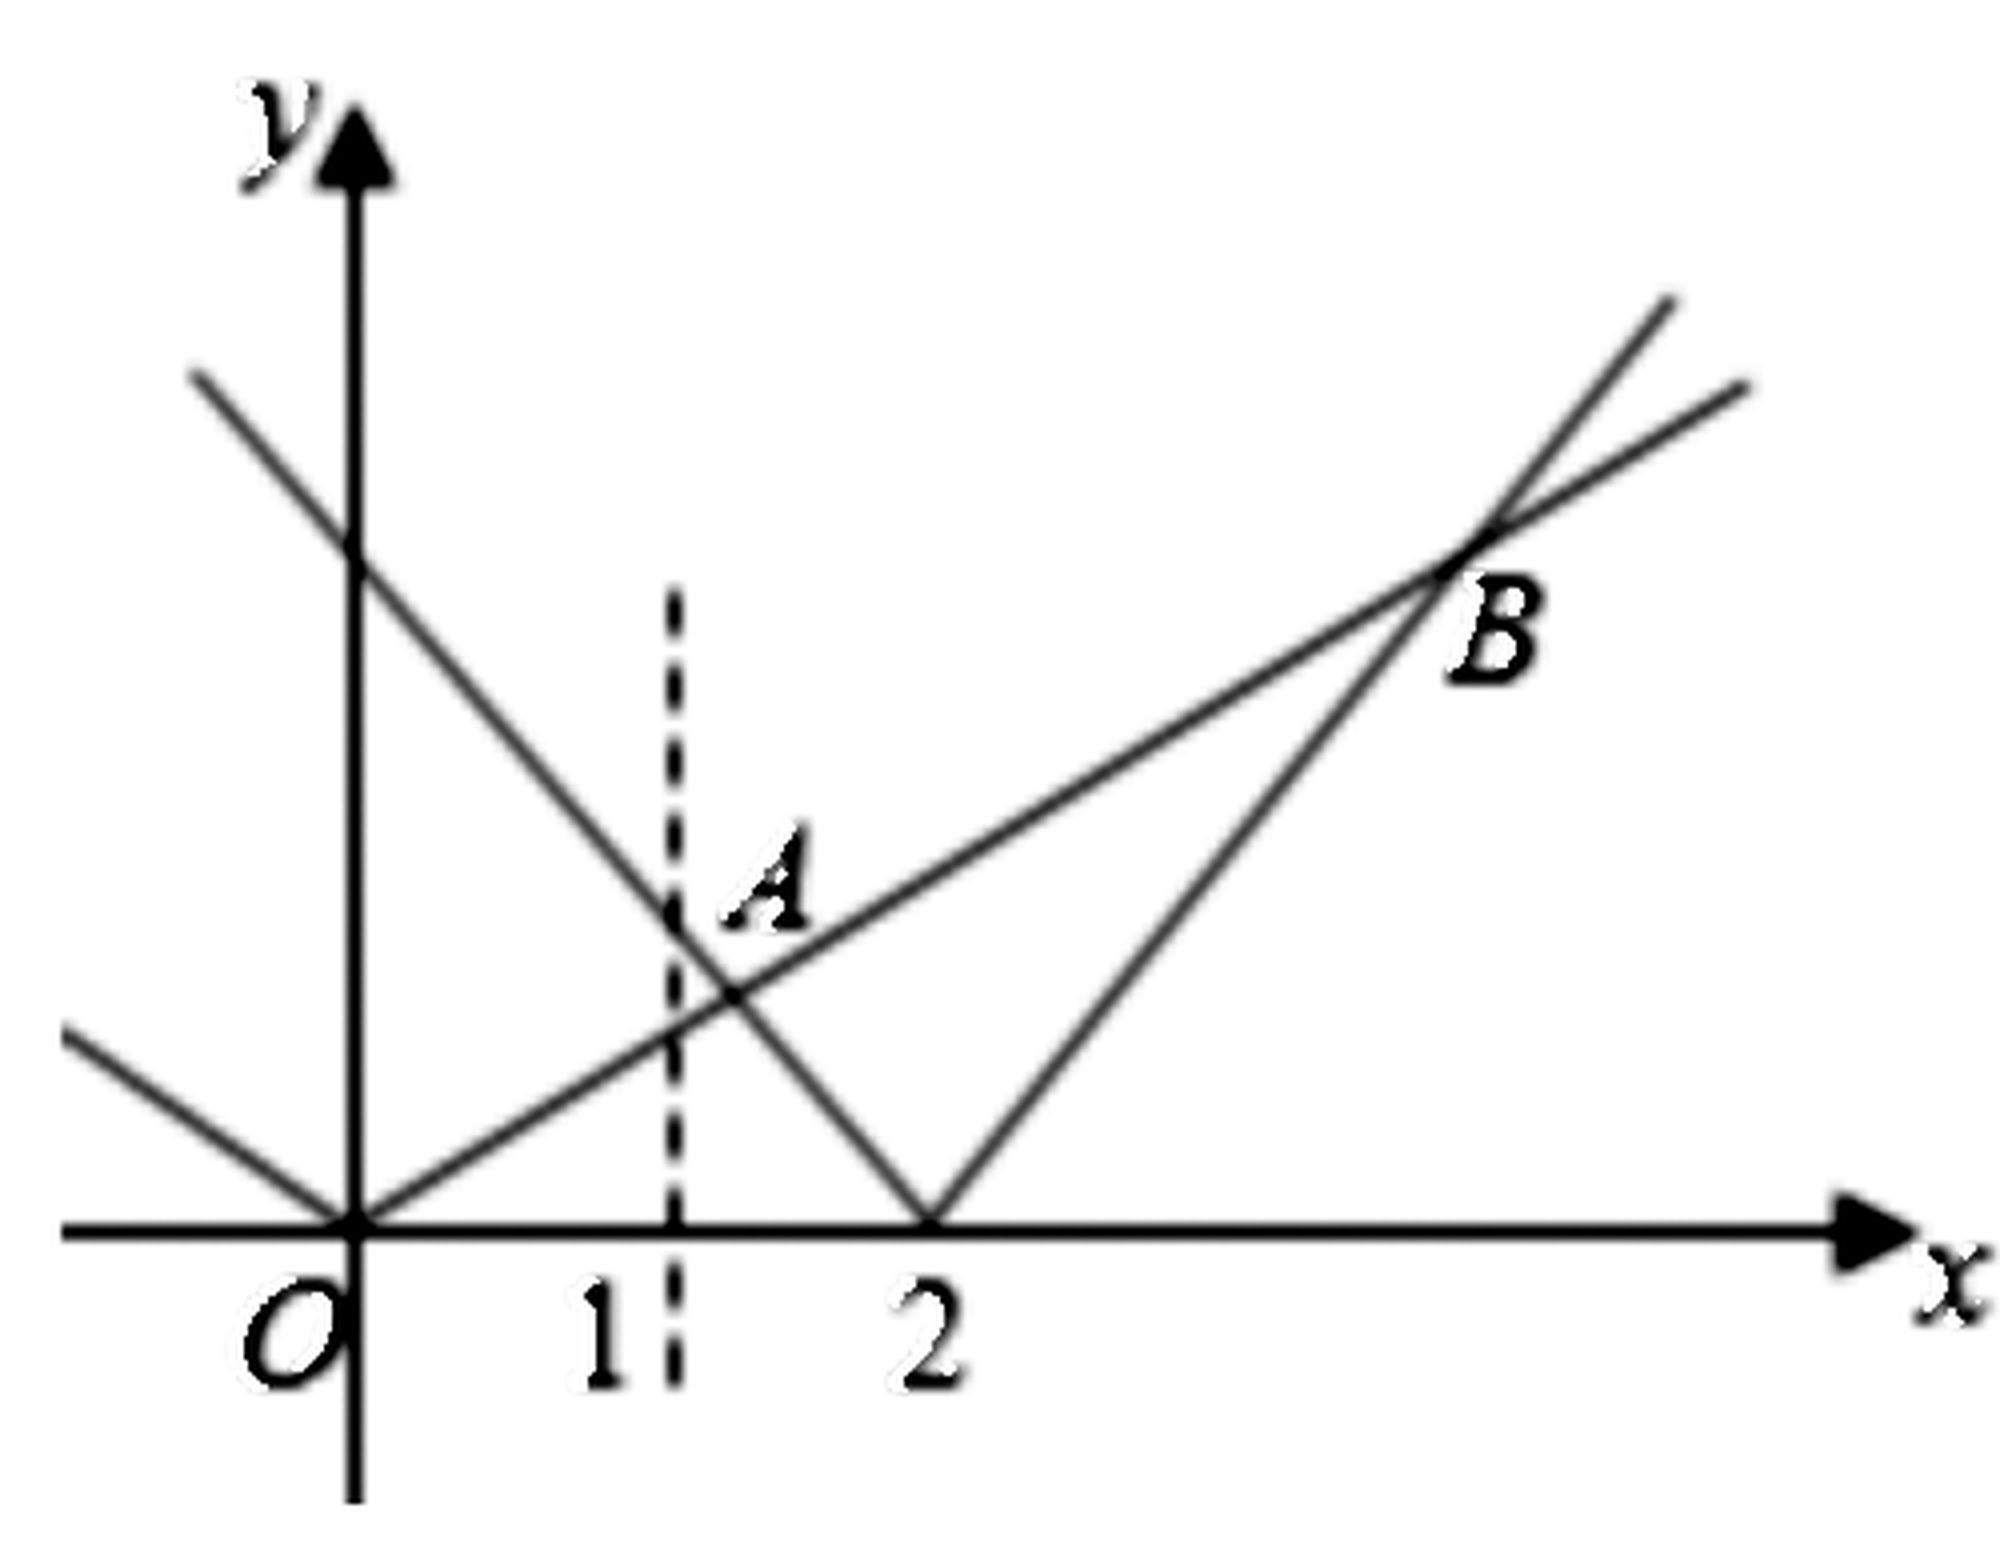
\includegraphics[width=0.40\textwidth]{figures/gao152_q15.png}
\end{center}
\step{由 $0<k<1$，得 $x_A>1$，}
\step{所以关于 $x$ 的不等式 $k\lvert x\rvert-\lvert x-2\rvert>0$ 恰好有 4 个整数解，是 2，3，4，5，}
\step{由 $\begin{cases}y=kx\\y=x-2\end{cases}\Rightarrow x_B=\dfrac2{1-k}\in(5,6]$，故 $\dfrac35<k\leqslant\dfrac23$；故选 $B$.}
\solend
\fi

% === Q16 === 咖啡优惠题；解析 12 行（跨 04 页上下半）；故选 C
\item 上海是全球咖啡店最多的城市. 若某品牌的某种在售咖啡产品价格为 30 元/杯，其原材料成本为 7 元/杯，营销成本为 5 元/杯，且该品牌门店提供如下 4 种优惠方式：(1) 首杯免单，每人限用一次；(2) 3.8 折优惠券，每人限用一次；(3) 买 2 杯送 2 杯，每人限用两次；(4) 买 5 杯送 5 杯，不限使用人数和使用次数. 每位消费者都可以在以上 4 种优惠方式中选择不多于 2 种使用. 现在某个公司有 5 位后勤工作人员去该品牌门店帮每位技术人员购买 1 杯咖啡，购买杯数与技术人员人数须保持一致；请问，这个公司的技术人员不少于\mbox{（\quad）}人时，无论 5 位后勤人员采用什么样的优惠方式购买咖啡，这笔订单该品牌门店都能保证盈利.

\keepwithprev
A. 20\qquad\qquad B. 25\qquad\qquad C. 30\qquad\qquad D. 35

\ifanswer
\solbegin
\step{按各优惠不叠加于同一杯理解，3.8 折券仅用于一杯，}
\step{买赠中的购买杯按原价付款.}
\step{设共购 $n$ 杯，免单、券购、原价购买的杯数分别为 $a,b,c$，其中 $0\leqslant a,b\leqslant5$，}
\step{其余为买赠咖啡，每杯成本为 12 元，}
\step{利润为 $P=15(n-a-b-c)+11.4b+30c-12n=3n-15a-3.6b+15c$，}
\step{若 $a,b$ 不同时为 5，则 $15a+3.6b\leqslant75+14.4=89.4$，}
\step{当 $n\geqslant30$ 时，$P\geqslant90-89.4=0.6>0$.}
\step{若 $a=b=5$，则每人均已使用免单和优惠券两种方式，其余均须原价购买，}
\step{$P=57+30(n-10)-12n=18n-243\geqslant297>0$.}
\step{当 $n=29$ 时，4 人各用方式 (1)(2) 购得 2 杯，}
\step{另 1 人用方式 (1) 及两次方式 (4) 购得 21 杯，}
\step{此时 $P=4\times11.4+2\times150-29\times12=-2.4<0$，因此最小人数为 30，故选 $C$.}% $2\times150$ 为两次方式（4）各买 5 杯的付款，照录（见 ⑤ 3）
\solend
\fi

\end{enumerate}

\bigsec{三、解答题}

\begin{enumerate}
\setcounter{enumi}{16}

% === Q17 === 解集含 \R／\varnothing；解析 4 行
\item 若 $a$、$b\in\R$，求关于 $x$ 的不等式 $ax\geqslant b$ 的解集.

\ifanswer
\solbegin
\step{当 $a>0$ 时，原不等式的解集为 $\left\{x\mid x\geqslant\dfrac ba\right\}$；}
\step{当 $a<0$ 时，原不等式的解集为 $\left\{x\mid x\leqslant\dfrac ba\right\}$；}
\step{当 $a=0$，$b\leqslant0$ 时，原不等式的解集为 $\R$；}
\step{当 $a=0$，$b>0$ 时，原不等式的解集为 $\varnothing$.}
\solend
\fi

% === Q18 === 子集 ⊆ 两处照录；cases 块；解析 9 行（跨 05 页上下半）
\item 已知 $\alpha:x<3m-1$ 或 $x>-m$，$\beta:x<2$ 或 $x\geqslant4$.

(1) 若 $\alpha$ 是 $\beta$ 的充分条件，求实数 $m$ 的取值范围；

(2) 若 $\alpha$ 是 $\beta$ 的必要条件，求实数 $m$ 的取值范围.

\ifanswer
\solbegin
\step{(1) 设 $A=\{x\mid x<3m-1\text{ 或 }x>-m\}$，$B=\{x\mid x<2\text{ 或 }x\geqslant4\}$，}
\step{因为 $\alpha$ 是 $\beta$ 的充分条件，所以 $A\subseteq B$，}
\step{当 $3m-1>-m$ 时，即 $m>\dfrac14$，此时 $A=\R$，不满足题意；}
\step{当 $3m-1\leqslant-m$ 时，即 $m\leqslant\dfrac14$，有 $\begin{cases}3m-1\leqslant2\\-m\geqslant4\end{cases}$，解得 $m\leqslant-4$；}
\step{综上，$m$ 的取值范围为 $(-\infty,-4]$.}
\step{(2) 因为 $\alpha$ 是 $\beta$ 的必要条件，所以 $B\subseteq A$，}
\step{当 $3m-1>-m$ 时，即 $m>\dfrac14$，此时 $A=\R$，$B\subseteq A$ 成立；}
\step{当 $3m-1\leqslant-m$ 时，即 $m\leqslant\dfrac14$，有 $\begin{cases}3m-1\geqslant2\\-m<4\end{cases}$，无解.}
\step{综上，$m$ 的取值范围为 $\left[\dfrac14,+\infty\right)$.}
\solend
\fi

% === Q19 === \varnothing 空集照录；解析 9 行
\item 设关于 $x$ 的不等式 $x^2+4x+k-1\geqslant0$ 的解集为 $A$.

(1) 若 $A=\R$，求实数 $k$ 的取值范围；

(2) 求证：不存在实数 $k$，使得 $A=\varnothing$.

\ifanswer
\solbegin
\step{(1) 配方得 $x^2+4x+k-1=(x+2)^2+k-5$，}
\step{若 $A=\R$，取 $x=-2$，得 $k-5\geqslant0$，即 $k\geqslant5$.}
\step{当 $k\geqslant5$ 时，对任意 $x\in\R$，都有 $(x+2)^2+k-5\geqslant0$，因此 $A=\R$.}
\step{所以 $k$ 的取值范围为 $[5,+\infty)$.}
\step{(2) 当 $k\geqslant5$ 时，由 (1) 得 $A=\R\ne\varnothing$.}
\step{当 $k<5$ 时，取 $x_0=-2+\sqrt{5-k}$，}
\step{则 $x_0^2+4x_0+k-1=(x_0+2)^2+k-5=(5-k)+k-5=0$，}
\step{所以 $x_0\in A$，即 $A\ne\varnothing$.}
\step{因此，不存在实数 $k$，使得 $A=\varnothing$.}
\solend
\fi

% === Q20 === |A\cap B|=1 印等号；等腰偏高粗 \Delta 照录；解析 12 行（跨 06→07 页）
\item 设 $m\in\R$. 集合 $A=\left\{x\mid\dfrac{x^2+x}{x+1}\geqslant\dfrac{2x+m}{x},x\in\R\right\}$，
$B=\left\{x\mid\dfrac{x^2+x}{x+1}\leqslant\dfrac{2x+m}{x},x\in\R\right\}$.

(1) 若 $m=8$，记集合 $M=A\cap(0,+\infty)$，求集合 $M$；

(2) 用 $\lvert T\rvert$ 代表集合 $T$ 的元素个数. 若 $\lvert A\cap B\rvert=1$，记 $m$ 的取值集合为 $C$，试比较 $\lvert C\rvert$ 与 2 的大小，并证明你的结论.

\ifanswer
\solbegin
\step{(1) 当 $m=8$，$x>0$ 时，$\dfrac{x^2+x}{x+1}\geqslant\dfrac{2x+8}{x}\Leftrightarrow x^2-2x-8\geqslant0$}
\step{$\Leftrightarrow(x-4)(x+2)\geqslant0\Leftrightarrow x\geqslant4$，所以 $M=[4,+\infty)$.}
\step{(2) 原分式有意义须 $x\ne-1,0$，因此 $x\in A\cap B\Leftrightarrow\begin{cases}x^2-2x-m=0\\x\ne-1,0\end{cases}$，}
\step{方程的判别式为 $\Delta=4(1+m)$.}
\step{当 $m<-1$ 时，方程无实根，$\lvert A\cap B\rvert=0$；}
\step{当 $m=-1$ 时，方程只有一个实根 1，$A\cap B=\{1\}$.}
\step{当 $m>-1$ 时，方程有两个不同实根.}
\step{其中，0 为根当且仅当 $m=0$，$-1$ 为根当且仅当 $m=3$.}
\step{$m=0$ 时，方程的根为 $0,2$，$A\cap B=\{2\}$；}
\step{$m=3$ 时，方程的根为 $-1,3$，$A\cap B=\{3\}$.}
\step{$m>-1$ 且 $m\ne0,3$ 时，两个实根均满足原分式的定义条件，$\lvert A\cap B\rvert=2$.}
\step{因此 $C=\{-1,0,3\}$，$\lvert C\rvert=3>2$.}
\solend
\fi

% === Q21 === "性质 p"新定义、\Q 归一、M\subseteq\R 照录；解析 19 行（跨 07→08 页）
\item 设集合 $M\subseteq\R$. 若 $M$ 中元素个数大于等于 2，且 $M$ 的任意不同元素 $a$、$b$ 均满足 $a^3-\dfrac14b\in M$，则称集合 $M$ 具有“性质 $p$”.

(1) 试判断集合 $\Q$、集合 $\left\{-\dfrac{\sqrt3}{2},0,\dfrac{\sqrt3}{2}\right\}$ 是否具有“性质 $p$”，并说明理由；

(2) 设 $m$ 为大于等于 2 的正整数. 若集合 $A=\{x_1,x_2,\cdots,x_m\}$，且具有“性质 $p$”，求证：$m=2$，并求集合 $A$ 中所有元素的乘积.

\ifanswer
\solbegin
\step{(1) $\Q$ 中至少有两个元素，且任意不同的 $a,b\in\Q$ 均满足 $a^3-\dfrac14b\in\Q$，}
\step{故 $\Q$ 具有“性质 $p$”.}
\step{对于另一集合，取 $a=0$，$b=\dfrac{\sqrt3}{2}$，则 $a^3-\dfrac14b=-\dfrac{\sqrt3}{8}$ 不属于该集合，}
\step{故其不具有“性质 $p$”.}
\step{(2) 将 $A$ 中元素按 $x_1<x_2<\cdots<x_m$ 排列.}
\step{若 $m\geqslant3$，由性质 $p$ 及幂函数 $y=x^3$ 的单调性，}
\step{有 $x_1^3-\dfrac14x_m<\cdots<x_1^3-\dfrac14x_2<x_m^3-\dfrac14x_2<x_m^3-\dfrac14x_1$，}
\step{上述 $m+1$ 个互不相同的数均属于 $A$，与 $A$ 只有 $m$ 个元素矛盾，}
\step{因此 $m=2$.}
\step{设 $A=\{a,b\}$，$a<b$.}
\step{因为 $a^3-\dfrac14b<b^3-\dfrac14a$，且两者均属于 $A$，}
\step{所以 $a^3-\dfrac14b=a$，$b^3-\dfrac14a=b$，}
\step{两式相减并除以 $a-b\ne0$，}
\step{以及两式相加，分别得 $a^2+ab+b^2=\dfrac34$，$(a+b)(a^2-ab+b^2)=\dfrac54(a+b)$，}
\step{代入 $a^2-ab+b^2=\dfrac34-2ab$，得 $(a+b)(4ab+1)=0$，}
\step{若 $a+b=0$，则 $-ab=a^2+ab+b^2=\dfrac34$，即 $ab=-\dfrac34$；}
\step{若 $a+b\ne0$，则 $ab=-\dfrac14$.}
\step{分别取 $A=\left\{-\dfrac{\sqrt3}{2},\dfrac{\sqrt3}{2}\right\}$，$A=\left\{\dfrac{1-\sqrt3}{2\sqrt2},\dfrac{1+\sqrt3}{2\sqrt2}\right\}$，}
\step{代入均有 $a^3-\dfrac14b=a$、$b^3-\dfrac14a=b$，故两种乘积均可取得.}
\solend
\fi

\end{enumerate}

\end{document}
"
% 紧凑版：xelatex "\def\iscompact{1}% 高一152_位育中学_期中.tex
%   —— 高一上数学"2026-2027 年位育中学高一上期中"（试卷版/答案版/紧凑版）
% 试卷版：xelatex 高一152_位育中学_期中.tex
% 答案版：xelatex "\def\isanswer{1}\input{高一152_位育中学_期中.tex}"
% 紧凑版：xelatex "\def\iscompact{1}\input{高一152_位育中学_期中.tex}"
%
% ① 原始材料：微信公众号"魔都数学加油站"文章，连载"27学年高一152"，原文标题
% "27学年高一152——2026-2027年上海市位育中学高一上期中"；
% 原文链接：https://mp.weixin.qq.com/s/v4_G6oTX2BuPz9L-KtLRfw 。
% 正文为 8 张 PNG 页（01/03/05/06/07/08 为 2560×3620，02/04 为 4762×6735，
% 同一篇各页分辨率混排，逐页按各自分辨率裁图核对，别按预览比例换算裁框）。
% 体例：讲评版——填空 3—12（10 题）、选择 13—16（4 题）、解答 17—21（5 题），
% 共 19 题，自第 3 题起编；题目、答案、解析均据原图转录；卷面粉红色水印
% "魔都数学加油站"及公众号页脚未录入。
% 全卷插图清单（逐页通读 8 页确认）：1 幅——第 15 题解析配图（两条折线
% $y=k\lvert x\rvert$ 与 $y=\lvert x-2\rvert$ 及坐标图，03 页右下，含 O、1、2、
% A、B 与虚线 $x=1$），解析写"的图象如下"，仅答案版出，裁
% figures/gao152_q15.png（去粉水印、去色、4× LANCZOS 放大）。
%
% 卷首标题：原卷印作"2026-2027 年位育中学高一上期中"，年份区间按全稿惯例排 en dash；
% 原卷卷面未印副标题，本稿按同期中卷知识模块口径补出"集合与常用逻辑用语、不等式、函数"。
%
% ② 与原卷的排版差异：
%   ① 原文从第 3 题起，本稿保留原题号；共 19 题三节，解答题 5 题到 21；
%   ② 混合体例：第 3、5 题只印【答案】、无【解析】，按 高一140 第 5 题／
%      高一145 第 3 题成例另提 \ans{}、不补造解析；第 13、14 题把答案"D"
%      直接印在题干括号内、题下无【解析】，按 高一84／148／149 成例括号留空、
%      另提 \ans{$D$}；其余 15 题印【解析】、用 \solbegin…\solend；
%      第 15、16 题答案在解析末句"故选 B／C"、括号留空、不另提 \ans{}；
%      答案版【答案】/【解析】标记数 = 19 = 全卷题数（4 个 \ans ＋ 15 个 \solbegin）；
%   ③ 原卷卷面未印副标题，本稿按知识模块口径补出；
%   ④ 原卷填空横线按全稿惯例排 \blankline[4.4em]；选择题括号排 \mbox{（\quad）}、
%      四道选择题的选项段前按惯例各加 \keepwithprev；解答题不留作答区、不加
%      \anspace（原卷为讲评版，109—113 起全稿不用 \anspace）；
%   ⑤ 数集黑板粗体：Q7"全集为 R"、Q9"$\lVert PQ\rVert$ 定义"无数集、
%      Q12"$t\in Z$"、Q13"$k\in Z$ 与 $=\R$"、Q17"$a,b\in R$"、Q19"$A=\R$"、
%      Q20"$m\in\R$"、Q21"$M\subseteq\R$ 与集合 $\Q$"原卷印正体粗体或黑板体
%      R/Q/Z，按全稿惯例归一 \R／\Q／\Z；绝对值排 \lvert…\rvert
%      （Q4、Q9、Q11、Q15），集合描述竖线排 \mid（Q7、Q13、Q20、Q21），
%      距离双竖线排 \lVert…\rVert（Q9 与题干、解析的 ||PQ||／||AB||）；
%      不等号按全稿惯例排 \leqslant／\geqslant；补集照原卷上划线排 \overline{A}
%      （Q7 题干＋解析）；空集 \varnothing（Q17、Q19）；
%      子集 Q18 两处、Q21 题干一处均印带下划线 ⊆、照录 \subseteq（见 ④），
%      本卷无单线 \subset 用例；
%   ⑥ 判别式 Δ/△ 两形混用逐处照录、不得统一：Q11 解析"判别式 △=k²−8k>0"
%      印扁等边细线三角、照录 \triangle，Q20 (2) 解析"判别式为 Δ=4(1+m)"
%      印等腰偏高粗三角、照录 \Delta（/tmp/gao152/z/zoom/q11_delta.png、
%      q20_delta.png 放大并与 151 卷同型并排比较）；
%   ⑦ 中文弯引号照录：Q11"长度"、Q21"性质 p"（题干、两问与解析多处）、
%      Q6 从">"、"<"、"≥"、"≤"中选符号、Q16"（1）…（4）"半角括号；
%      注释里一律 ASCII 引号；数学式内 CJK 用 \text{}（Q13 的"或／且"、
%      Q18 集合描述的"或"）；
%   ⑧ "图像／图象"：全卷仅 Q15 解析一处"的图象如下"，印"图象"（象，无亻）、
%      照录；其余各题无"图像"字样。子题标号 (1)(2)(3)(4) 半角括号照录；
%   ⑨ 半角逗号在数学组之间是全稿惯例、非笔误，逐处照录（Q6、Q10、Q16、
%      Q20、Q21 的 $a,b,c$ 之类）；行末西文句点 ASCII `.`；
%      行中全角逗号／顿号照录（Q11"（a,b）"、Q16"7 元/杯"、Q21"$\Q$、集合"）；
%   ⑩ 复杂式照录别简化：Q4 四组 cases 块（整体各占一个印刷行）、Q8
%      $\frac{x_0}{e^{x_0}}=\frac13$、Q10 $4a^2+b^2=4$、Q12 $b=\frac2a$、
%      Q16 利润式 $P=15(n-a-b-c)+11.4b+30c-12n$、Q18 cases 块、
%      Q20 分式 $\frac{x^2+x}{x+1}$、Q21 $a^3-\frac14b$ 与两组取值集合；
%      \left…\right 不得拆到不同 $…$ 组（Q4 cases 前的 \left\{ 一律改
%      \begin{cases}…\end{cases}、Q17 $\left\{x\mid x\ge\frac ba\right\}$、
%      Q20 $\left\{x\mid\cdots\right\}$、Q21 $\left\{-\frac{\sqrt3}2,\ldots\right\}$）；
%   ⑪ 一条 \step = 原卷解析的一个印刷行，cases 块整体算一个印刷行；别并折行、
%      别拆行。Q12 七行、Q16 十二行、Q18 九行、Q19 九行、Q20 十二行、
%      Q21 十九行均按印刷行逐条断，不丢行；
%   ⑫ 配图：Q15 解析配图（仅答案版出）放 \ifanswer 内 \solbegin…\solend 的
%      \step 之间（高一73 第 16 题／高一150 Q12 成例）；题干无配图，故无
%      \needvspace；
%   ⑬ 原卷解析内无红色"法一／法二"之类小标题，故本卷无 \stepm；红色水印
%      "魔都数学加油站"不录入；
%   ⑭ 跨页续印按题合并：见 ⑥；
%
% ③ 行数复核：一条 \step = 原卷解析的一个印刷行，cases 块作一个印刷行计。
%   逐题数（主会话逐页核对定稿）：Q3：0（只印【答案】、提 \ans{}）；Q4：2；
%   Q5：0（只印【答案】、提 \ans{}）；Q6：1；Q7：1；Q8：1；Q9：1；
%   Q10：4；Q11：5；Q12：7；Q13：0（答案印括号内、提 \ans{}）；
%   Q14：0（答案印括号内、提 \ans{}）；Q15：4；Q16：12；Q17：4；
%   Q18：9；Q19：9；Q20：12；Q21：19。
%   合计 91 条 \step（本卷无 \stepm），与原卷逐题印刷行相等。全卷 15 题设
%   \solbegin…\solend ＋ Q3／Q5／Q13／Q14 四处 \ans{}，答案版
%   【答案】/【解析】标记数 = 19 = 全卷题数。
%
% ④ 判别式／子集符号结论（逐处放大原图照录、不得统一，主会话像素级复核）：
%   判别式：Q11 解析"方程 $x^2-kx+2k=0$ 的判别式 $\triangle=k^2-8k>0$"
%      印扁等边细线三角、照录 \triangle；Q20 (2) 解析"方程的判别式为
%      $\Delta=4(1+m)$"印等腰偏高粗三角、照录 \Delta
%      （/tmp/gao152/z/zoom/q11_delta.png、q20_delta.png；与 高一142／151
%      的"Δ/△ 混用逐处照录"口径一致）。本卷无几何三角形符号。
%   子集：Q18 解析 (1)"$A\subseteq B$"、(2)"$B\subseteq A$"与 Q21 题干
%      "$M\subseteq\R$"共 3 处均印带下划线 ⊆、照录 \subseteq
%      （/tmp/gao152/z/zoom/q18_subset.png、q21_subset.png 放大确认）；
%      本卷无单线 ⊂ 用例。补集上划线 \overline{A}（Q7）、空集 \varnothing
%      （Q17 解析末行、Q19 题干 (2) 与解析）、数集 \R／\Q／\Z 归一见 ② ⑤。
%
% ⑤ 存疑照录（放大原图确认，照录未改、正文对应处另有 % 注）：
%   1. Q11 题干"已知关于 $x$ 的不等式 $x^2-kx+2k<0$ 有实数解，且解集区间
%      长度不超过 3 个单位"，解析据 $\lvert x_1-x_2\rvert\leqslant3$ 推；
%      判别式用扁三角 \triangle（见 ④），照录未改。
%   2. Q12 解析"$t=-1$ 时取 $b=\frac2a\in[-2,-1]$，$c=-1$，则 $ab+c=2-1=1$"
%      ——$b$ 径写 $\frac2a$（无负号），放大 03 页确认，照录未改。
%   3. Q16 解析"$P=4\times11.4+2\times150-29\times12=-2.4<0$"中的
%      $2\times150$ 为两次方式（4）各买 5 杯的付款，照录未改。
%   4. Q20 (2) 题干"若 $\lvert A\cap B\rvert=1$"印等号（非 $\leqslant1$），
%      放大 06 页 /tmp/gao152/z/zoom/q20_eq1.png 确认，照录未改。
%   5. Q21 题干"性质 p"用弯引号且 $p$ 为斜体小写，逐处照录未统一；
%      解析 (2) 末两组 $A$ 的取值集合照录未简化。
%   6. "图像／图象"仅 Q15 一处"图象"、Δ/△ 两形并用（Q11 \triangle、
%      Q20 \Delta）均逐处照录、未统一（见 ② ⑥ ⑧ 与 ④）。
%   全卷除此 6 类外未发现其它笔误／自相矛盾处；19 题中 15 题印【解析】、
%   Q3／Q5 只印【答案】、Q13／Q14 答案印题干括号内（见 ② ②）。
%
% ⑥ 跨页续印按题合并说明（逐页核实定稿）：Q3—Q5 题干＋【答案】／【解析】
%   在 01 页上半，Q6—Q8 题干＋解析在 01 页下半；Q9、Q10 题干＋解析、
%   Q11 题干＋解析、Q12 题干＋解析首行在 02 页；Q12 解析余 6 行续 03 页
%   上半，"二、选择题"标题与 Q13 题干＋选项在 03 页下半；Q13 选项 C／D、
%   Q14 题干＋四选项＋（无解析）、Q15 题干＋四选项＋解析前 3 行＋配图在
%   03 页下半，Q15 解析末行（由 cases 求 $x_B$）续 04 页顶；Q16 题干＋四选项
%   ＋解析前 5 行在 04 页上半，解析余 7 行在 04 页下半；"三、解答题"标题与
%   Q17 题干＋解析首行在 04 页末，Q17 解析余 3 行、Q18 题干＋两问＋解析首
%   4 行在 05 页上半，Q18 解析余 5 行在 05 页下半；Q19 题干＋两问＋解析
%   (1) 4 行在 05—06 页（(2) 题干续 06 页顶），解析 (2) 5 行在 06 页上半；
%   Q20 题干＋两问＋解析 (1) 2 行＋(2) 首行在 06 页下半；Q20 (2) 解析余
%   9 行、Q21 题干＋两问＋解析 (1) 4 行在 07 页；Q21 (2) 解析 19 行中前
%   6 行在 07—08 页上半、末 13 行续 08 页下半，末行"故两种乘积均可取得"
%   为全卷收尾（08 页下半仅水印、无其它正文）。
%   本稿按题连排，不丢行、不并折行；全卷末题为第 21 题，无附加题节。
%
\documentclass[a4paper,11pt]{article}
\usepackage{common}

\begin{document}

\examtitlest[3]{2026--2027 年位育中学高一上期中}{集合与常用逻辑用语、不等式、函数}

\bigsec{一、填空题}

\begin{enumerate}
\setcounter{enumi}{2}

% === Q3 === 原卷只印【答案】、无【解析】，另提 \ans{}，不补造解析
\item 设 $x>0$. 若 $\ln x=-1$，则 $x=$\blankline[4.4em].

\ifanswer
\ans{$\dfrac1{\mathrm{e}}$}
\fi

% === Q4 === 四组 cases 块同一印刷行；解析 2 行
\item 不等式 $\lvert 1-2x\rvert>x$ 的解集为\blankline[4.4em].

\ifanswer
\solbegin
\step{不等式 $\lvert 1-2x\rvert>x$ 即为 $\begin{cases}1-2x\geqslant0\\1-2x>x\end{cases}$ 或 $\begin{cases}1-2x<0\\2x-1>x\end{cases}$，即 $\begin{cases}x\leqslant\frac12\\x<\frac13\end{cases}$ 或 $\begin{cases}x>\frac12\\x>1\end{cases}$，}
\step{则有 $x<\dfrac13$ 或 $x>1$，则解集为 $\left(-\infty,\dfrac13\right)\cup(1,+\infty)$.}
\solend
\fi

% === Q5 === 原卷只印【答案】、无【解析】；\frac1x\ge1 印单线 ≥，按全稿惯例 \geqslant
\item 不等式 $\dfrac1x\geqslant1$ 的解集为\blankline[4.4em].

\ifanswer
\ans{$(0,1]$}
\fi

% === Q6 === 从四个符号中选一个，中文弯引号照录；解析 1 行
\item 设 $a$、$b>0$，则 $a^2+b^2$\blankline[4.4em]$2(2a-b)-5$（从“$>$”、“$<$”、“$\geqslant$”、“$\leqslant$”中选择一个符号填写）.

\ifanswer
\solbegin
\step{$a^2+b^2-[2(2a-b)-5]=(a-2)^2+(b+1)^2>0$，故 $a^2+b^2>2(2a-b)-5$.}
\solend
\fi

% === Q7 === 补集上划线 \overline{A}；集合描述竖线 \mid；解析 1 行
\item 已知全集为 $\R$，集合 $A=\{x\mid y=\sqrt{x-2}\}$，集合 $B=\{y\mid y=\sqrt{x-2}\}$，则 $\overline{A}\cap B=$\blankline[4.4em].

\ifanswer
\solbegin
\step{$A=[2,+\infty)$，$B=[0,+\infty)$，所以 $\overline{A}\cap B=[0,2)$.}
\solend
\fi

% === Q8 === \frac{x_0}{e^{x_0}}=\frac13 照录；解析 1 行
\item 设正数 $x_0$ 满足等式 $\dfrac{x_0}{e^{x_0}}=\dfrac13$，则 $x_0-\ln x_0=$\blankline[4.4em].

\ifanswer
\solbegin
\step{等式两边取自然对数，得 $\ln x_0-x_0=-\ln3$，即 $x_0-\ln x_0=\ln3$.}
\solend
\fi

% === Q9 === 距离双竖线 \lVert…\rVert；解析 1 行
\item 在平面直角坐标系 $xOy$ 中，设点 $P(x_1,y_1)$，$Q(x_2,y_2)$，定义：$\lVert PQ\rVert=\lvert x_1-x_2\rvert+\lvert y_1-y_2\rvert$. 若点 $A(1,0)$，点 $B$ 为直线 $y=x+2$ 上的动点，则 $\lVert AB\rVert$ 的最小值为\blankline[4.4em].

\ifanswer
\solbegin
\step{$\lVert AB\rVert=\lvert x-1\rvert+\lvert y\rvert=\lvert x-1\rvert+\lvert x+2\rvert\geqslant3$，最小值为 3.}
\solend
\fi

% === Q10 === 解析 4 行
\item 已知 $a$、$b$ 均为正数，且 $a^2+\dfrac14b^2=1$，则 $a\sqrt{1+b^2}$ 的最大值为\blankline[4.4em].

\ifanswer
\solbegin
\step{因为 $a$、$b$ 均为正数，且 $a^2+\dfrac14b^2=1$，所以 $4a^2+b^2=4$，}
\step{所以 $a\sqrt{1+b^2}=\dfrac12\cdot2a\cdot\sqrt{1+b^2}\leqslant\dfrac12\cdot\dfrac{4a^2+1+b^2}{2}=\dfrac54$，}
\step{当且仅当 $4a^2=b^2+1$ 即 $a=\dfrac{\sqrt{10}}4$，$b=\dfrac{\sqrt6}2$ 时取等号，}
\step{故 $a\sqrt{1+b^2}$ 的最大值为 $\dfrac54$.}
\solend
\fi

% === Q11 === 扁等边细线判别式 \triangle 照录（见 ④）；"长度"弯引号；解析 5 行
\item 一般地，把 $b-a$ 称为区间 $(a,b)$ 的“长度”. 已知关于 $x$ 的不等式 $x^2-kx+2k<0$ 有实数解，且解集区间长度不超过 3 个单位，则实数 $k$ 的取值范围是\blankline[4.4em].

\ifanswer
\solbegin
\step{因为不等式 $x^2-kx+2k<0$ 有解，}
\step{所以方程 $x^2-kx+2k=0$ 的判别式 $\triangle=k^2-8k>0$，解得 $k>8$ 或 $k<0$，}
\step{由 $x_1+x_2=k$，$x_1x_2=2k$，得 $(x_1-x_2)^2=(x_1+x_2)^2-4x_1x_2=k^2-8k$，}
\step{由 $\lvert x_1-x_2\rvert\leqslant3$，得 $(x_1-x_2)^2\leqslant9$，即 $k^2-8k\leqslant9$，解得 $-1\leqslant k\leqslant9$，}
\step{所以 $-1\leqslant k<0$ 或 $8<k\leqslant9$，即实数 $k$ 的取值范围是 $[-1,0)\cup(8,9]$.}
\solend
\fi

% === Q12 === $b=\frac2a$ 无负号、$c=-1$ 照录（见 ⑤ 2）；解析 7 行（跨 02→03 页）
\item 设 $t\in\Z$，且对任意 $a\in[-2,t]$，总存在 $b,c\in[-2,t]$，使得 $ab+c=1$，则 $t$ 的所有取值为\blankline[4.4em].

\ifanswer
\solbegin
\step{$[-2,t]$ 是区间，要求 $t>-2$，故 $t\geqslant-1$.}
\step{当 $t\geqslant1$ 时，对任意 $a\in[-2,t]$，}
\step{取 $b=0$，$c=1$，两者都属于 $[-2,t]$，且 $ab+c=1$.}
\step{当 $t=0$ 时，取 $a=0$，则 $c=1\notin[-2,0]$，不成立.}
\step{当 $t=-1$ 时，对任意 $a\in[-2,-1]$，取 $b=\dfrac2a\in[-2,-1]$，$c=-1$，}% 原卷径写 $b=\frac2a$（无负号），放大 03 页确认，照录未改（见 ⑤ 2）
\step{则 $ab+c=2-1=1$.}
\step{所以 $t=-1$ 或 $t\geqslant1$（$t\in\Z$）.}
\solend
\fi

\end{enumerate}

\bigsec{二、选择题}

\begin{enumerate}
\setcounter{enumi}{12}

% === Q13 === 答案 D 印在题干括号内、无【解析】，按 高一84／148／149 成例括号留空、另提 \ans{}
\item 下列说法错误的是\mbox{（\quad）}

\keepwithprev
A. 奇数集可以表示为 $\{x\mid x=2k+1,k\in\Z\}$

B. 奇数集可以表示为 $\{x\mid x=2k-1,k\in\Z\}$

C. $\{x\mid x\ne2\text{ 或 }x\ne-2\}=\R$

D. $\{x\mid x\ne2\text{ 且 }x\ne-2\}=\R$

\ifanswer
\ans{$D$}
\fi

% === Q14 === 答案 D 印在题干括号内、无【解析】；选项两行两列
\item 设 $a$、$b$、$c>0$，且 $a\ne1$，则以下代数式中，不恒成立的是\mbox{（\quad）}

\keepwithprev
A. $\log_a 1=0$\qquad\qquad B. $a^{\log_a b}=b$

C. $\log_a b+\log_a c=\log_a(bc)$\qquad\qquad D. $\log_a b=\dfrac1{\log_b a}$

\ifanswer
\ans{$D$}
\fi

% === Q15 === "图象"（象，无亻）照录；解析配图仅答案版出；答案在解析末句故选 B
\item 若关于 $x$ 的不等式 $k\lvert x\rvert>\lvert x-2\rvert$ 恰好有 4 个整数解，则实数 $k$ 的取值范围是\mbox{（\quad）}

\keepwithprev
A. $\left(\dfrac35,\dfrac23\right)$\qquad B. $\left(\dfrac35,\dfrac23\right]$\qquad C. $\left(\dfrac35,1\right)$\qquad D. $\left(\dfrac35,1\right]$

\ifanswer
\solbegin
\step{由题意得 $0<k<1$，函数 $y=k\lvert x\rvert$ 与 $y=\lvert x-2\rvert$ 的图象如下，}
\begin{center}
% 两条折线坐标图取 03 页右下，去粉色水印、去色、4× LANCZOS 放大；仅答案版出
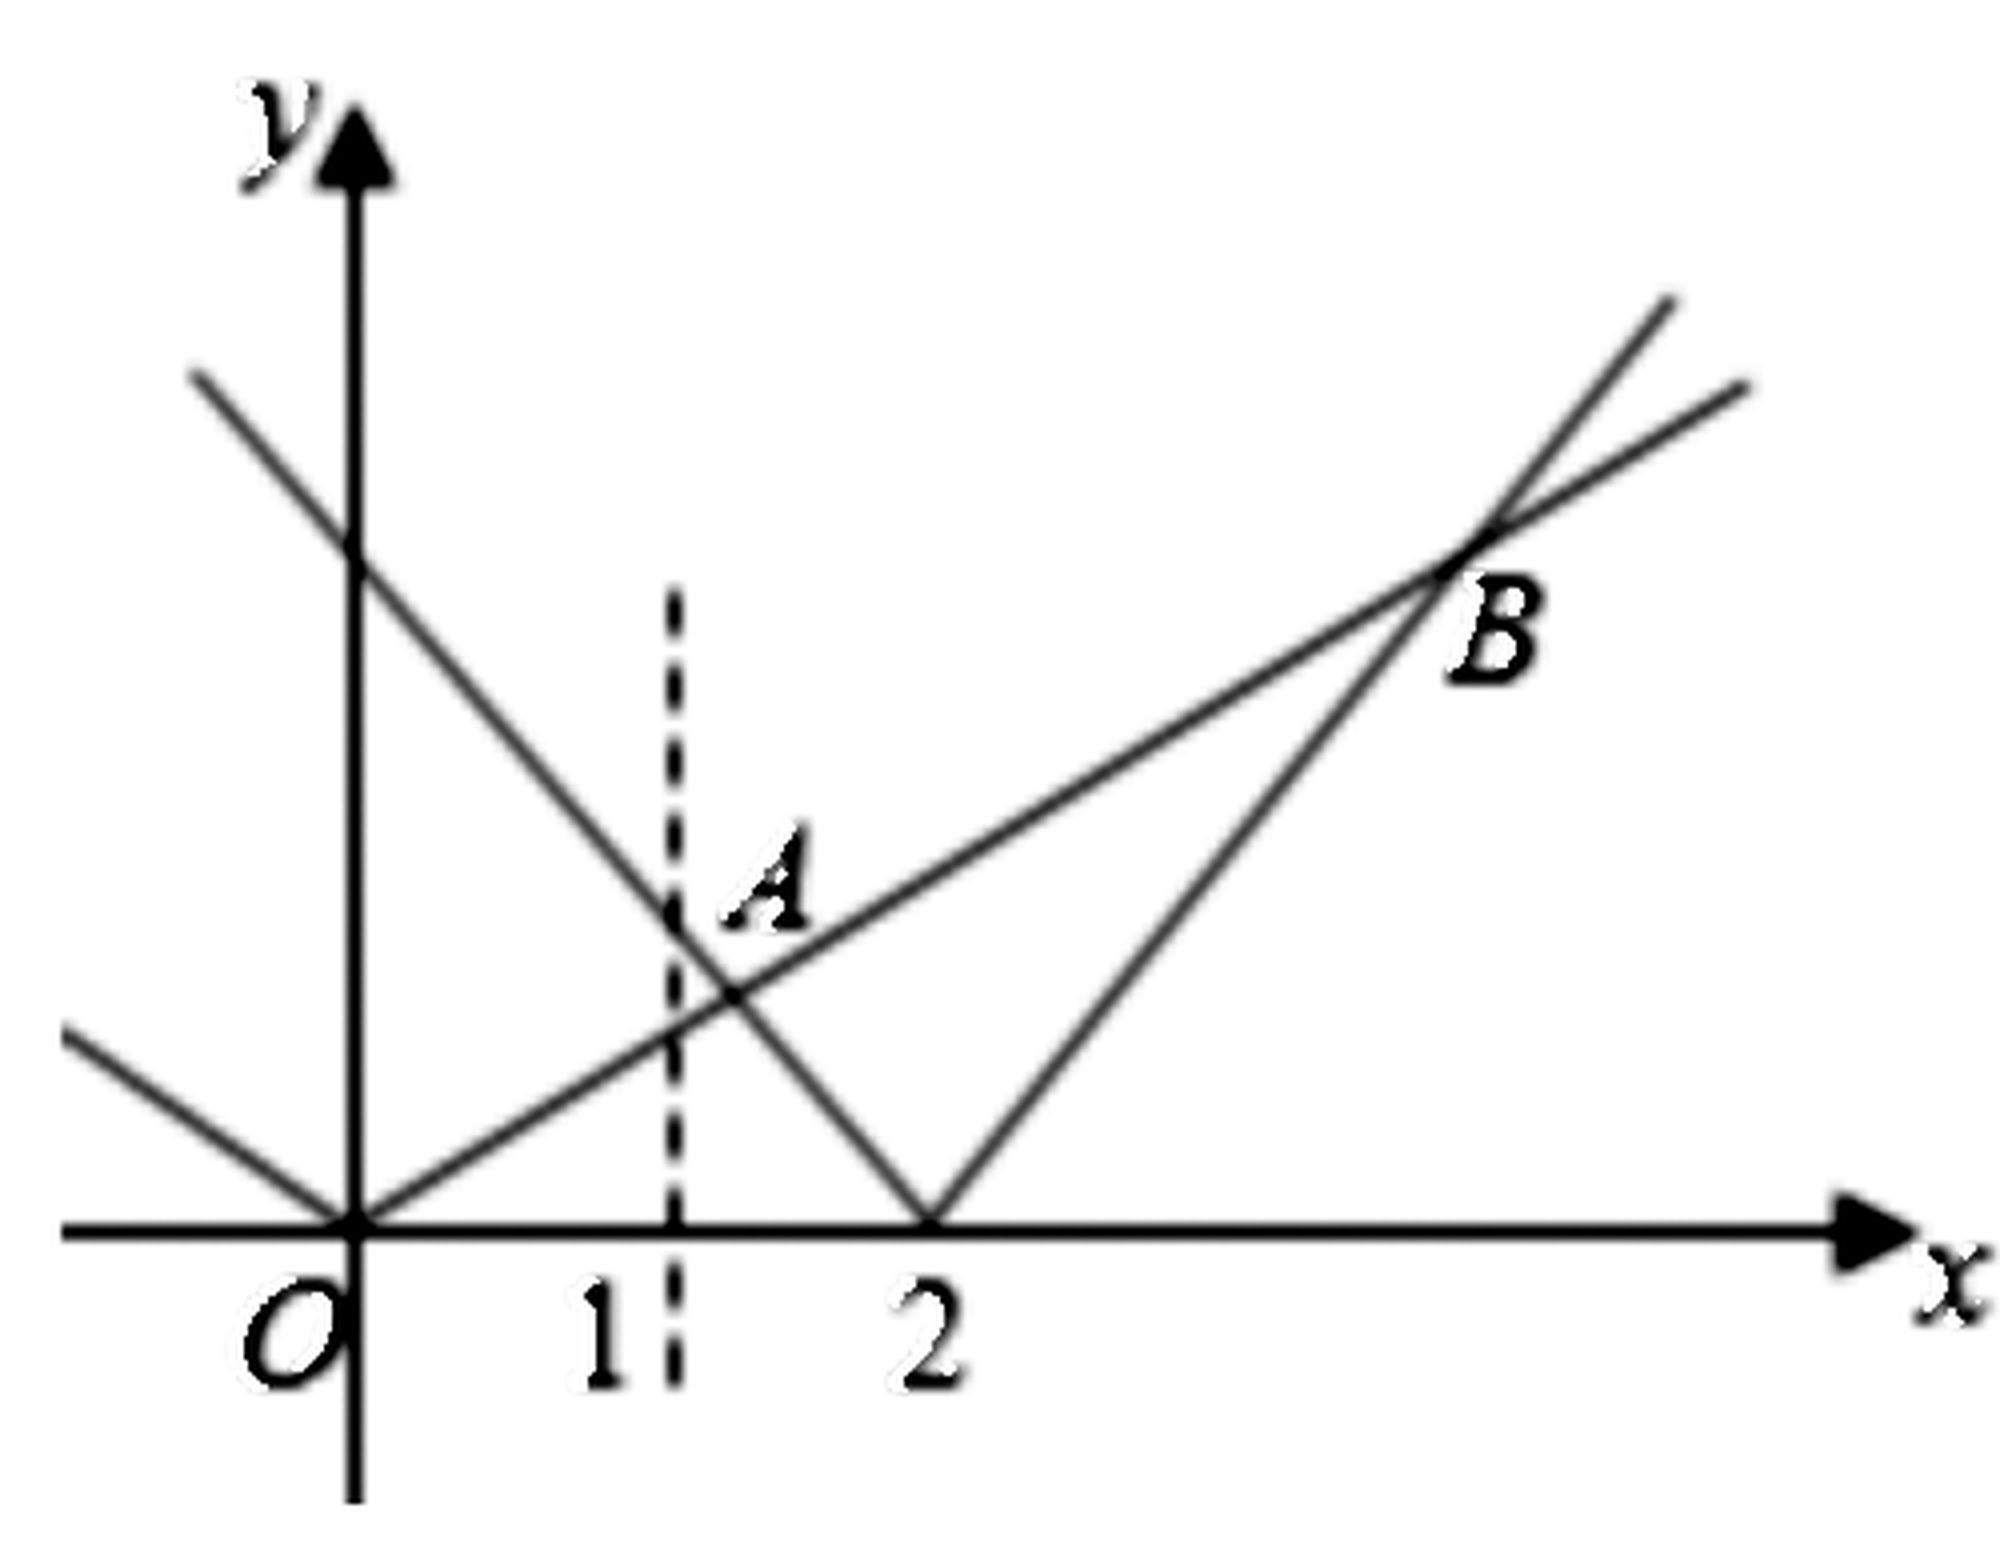
\includegraphics[width=0.40\textwidth]{figures/gao152_q15.png}
\end{center}
\step{由 $0<k<1$，得 $x_A>1$，}
\step{所以关于 $x$ 的不等式 $k\lvert x\rvert-\lvert x-2\rvert>0$ 恰好有 4 个整数解，是 2，3，4，5，}
\step{由 $\begin{cases}y=kx\\y=x-2\end{cases}\Rightarrow x_B=\dfrac2{1-k}\in(5,6]$，故 $\dfrac35<k\leqslant\dfrac23$；故选 $B$.}
\solend
\fi

% === Q16 === 咖啡优惠题；解析 12 行（跨 04 页上下半）；故选 C
\item 上海是全球咖啡店最多的城市. 若某品牌的某种在售咖啡产品价格为 30 元/杯，其原材料成本为 7 元/杯，营销成本为 5 元/杯，且该品牌门店提供如下 4 种优惠方式：(1) 首杯免单，每人限用一次；(2) 3.8 折优惠券，每人限用一次；(3) 买 2 杯送 2 杯，每人限用两次；(4) 买 5 杯送 5 杯，不限使用人数和使用次数. 每位消费者都可以在以上 4 种优惠方式中选择不多于 2 种使用. 现在某个公司有 5 位后勤工作人员去该品牌门店帮每位技术人员购买 1 杯咖啡，购买杯数与技术人员人数须保持一致；请问，这个公司的技术人员不少于\mbox{（\quad）}人时，无论 5 位后勤人员采用什么样的优惠方式购买咖啡，这笔订单该品牌门店都能保证盈利.

\keepwithprev
A. 20\qquad\qquad B. 25\qquad\qquad C. 30\qquad\qquad D. 35

\ifanswer
\solbegin
\step{按各优惠不叠加于同一杯理解，3.8 折券仅用于一杯，}
\step{买赠中的购买杯按原价付款.}
\step{设共购 $n$ 杯，免单、券购、原价购买的杯数分别为 $a,b,c$，其中 $0\leqslant a,b\leqslant5$，}
\step{其余为买赠咖啡，每杯成本为 12 元，}
\step{利润为 $P=15(n-a-b-c)+11.4b+30c-12n=3n-15a-3.6b+15c$，}
\step{若 $a,b$ 不同时为 5，则 $15a+3.6b\leqslant75+14.4=89.4$，}
\step{当 $n\geqslant30$ 时，$P\geqslant90-89.4=0.6>0$.}
\step{若 $a=b=5$，则每人均已使用免单和优惠券两种方式，其余均须原价购买，}
\step{$P=57+30(n-10)-12n=18n-243\geqslant297>0$.}
\step{当 $n=29$ 时，4 人各用方式 (1)(2) 购得 2 杯，}
\step{另 1 人用方式 (1) 及两次方式 (4) 购得 21 杯，}
\step{此时 $P=4\times11.4+2\times150-29\times12=-2.4<0$，因此最小人数为 30，故选 $C$.}% $2\times150$ 为两次方式（4）各买 5 杯的付款，照录（见 ⑤ 3）
\solend
\fi

\end{enumerate}

\bigsec{三、解答题}

\begin{enumerate}
\setcounter{enumi}{16}

% === Q17 === 解集含 \R／\varnothing；解析 4 行
\item 若 $a$、$b\in\R$，求关于 $x$ 的不等式 $ax\geqslant b$ 的解集.

\ifanswer
\solbegin
\step{当 $a>0$ 时，原不等式的解集为 $\left\{x\mid x\geqslant\dfrac ba\right\}$；}
\step{当 $a<0$ 时，原不等式的解集为 $\left\{x\mid x\leqslant\dfrac ba\right\}$；}
\step{当 $a=0$，$b\leqslant0$ 时，原不等式的解集为 $\R$；}
\step{当 $a=0$，$b>0$ 时，原不等式的解集为 $\varnothing$.}
\solend
\fi

% === Q18 === 子集 ⊆ 两处照录；cases 块；解析 9 行（跨 05 页上下半）
\item 已知 $\alpha:x<3m-1$ 或 $x>-m$，$\beta:x<2$ 或 $x\geqslant4$.

(1) 若 $\alpha$ 是 $\beta$ 的充分条件，求实数 $m$ 的取值范围；

(2) 若 $\alpha$ 是 $\beta$ 的必要条件，求实数 $m$ 的取值范围.

\ifanswer
\solbegin
\step{(1) 设 $A=\{x\mid x<3m-1\text{ 或 }x>-m\}$，$B=\{x\mid x<2\text{ 或 }x\geqslant4\}$，}
\step{因为 $\alpha$ 是 $\beta$ 的充分条件，所以 $A\subseteq B$，}
\step{当 $3m-1>-m$ 时，即 $m>\dfrac14$，此时 $A=\R$，不满足题意；}
\step{当 $3m-1\leqslant-m$ 时，即 $m\leqslant\dfrac14$，有 $\begin{cases}3m-1\leqslant2\\-m\geqslant4\end{cases}$，解得 $m\leqslant-4$；}
\step{综上，$m$ 的取值范围为 $(-\infty,-4]$.}
\step{(2) 因为 $\alpha$ 是 $\beta$ 的必要条件，所以 $B\subseteq A$，}
\step{当 $3m-1>-m$ 时，即 $m>\dfrac14$，此时 $A=\R$，$B\subseteq A$ 成立；}
\step{当 $3m-1\leqslant-m$ 时，即 $m\leqslant\dfrac14$，有 $\begin{cases}3m-1\geqslant2\\-m<4\end{cases}$，无解.}
\step{综上，$m$ 的取值范围为 $\left[\dfrac14,+\infty\right)$.}
\solend
\fi

% === Q19 === \varnothing 空集照录；解析 9 行
\item 设关于 $x$ 的不等式 $x^2+4x+k-1\geqslant0$ 的解集为 $A$.

(1) 若 $A=\R$，求实数 $k$ 的取值范围；

(2) 求证：不存在实数 $k$，使得 $A=\varnothing$.

\ifanswer
\solbegin
\step{(1) 配方得 $x^2+4x+k-1=(x+2)^2+k-5$，}
\step{若 $A=\R$，取 $x=-2$，得 $k-5\geqslant0$，即 $k\geqslant5$.}
\step{当 $k\geqslant5$ 时，对任意 $x\in\R$，都有 $(x+2)^2+k-5\geqslant0$，因此 $A=\R$.}
\step{所以 $k$ 的取值范围为 $[5,+\infty)$.}
\step{(2) 当 $k\geqslant5$ 时，由 (1) 得 $A=\R\ne\varnothing$.}
\step{当 $k<5$ 时，取 $x_0=-2+\sqrt{5-k}$，}
\step{则 $x_0^2+4x_0+k-1=(x_0+2)^2+k-5=(5-k)+k-5=0$，}
\step{所以 $x_0\in A$，即 $A\ne\varnothing$.}
\step{因此，不存在实数 $k$，使得 $A=\varnothing$.}
\solend
\fi

% === Q20 === |A\cap B|=1 印等号；等腰偏高粗 \Delta 照录；解析 12 行（跨 06→07 页）
\item 设 $m\in\R$. 集合 $A=\left\{x\mid\dfrac{x^2+x}{x+1}\geqslant\dfrac{2x+m}{x},x\in\R\right\}$，
$B=\left\{x\mid\dfrac{x^2+x}{x+1}\leqslant\dfrac{2x+m}{x},x\in\R\right\}$.

(1) 若 $m=8$，记集合 $M=A\cap(0,+\infty)$，求集合 $M$；

(2) 用 $\lvert T\rvert$ 代表集合 $T$ 的元素个数. 若 $\lvert A\cap B\rvert=1$，记 $m$ 的取值集合为 $C$，试比较 $\lvert C\rvert$ 与 2 的大小，并证明你的结论.

\ifanswer
\solbegin
\step{(1) 当 $m=8$，$x>0$ 时，$\dfrac{x^2+x}{x+1}\geqslant\dfrac{2x+8}{x}\Leftrightarrow x^2-2x-8\geqslant0$}
\step{$\Leftrightarrow(x-4)(x+2)\geqslant0\Leftrightarrow x\geqslant4$，所以 $M=[4,+\infty)$.}
\step{(2) 原分式有意义须 $x\ne-1,0$，因此 $x\in A\cap B\Leftrightarrow\begin{cases}x^2-2x-m=0\\x\ne-1,0\end{cases}$，}
\step{方程的判别式为 $\Delta=4(1+m)$.}
\step{当 $m<-1$ 时，方程无实根，$\lvert A\cap B\rvert=0$；}
\step{当 $m=-1$ 时，方程只有一个实根 1，$A\cap B=\{1\}$.}
\step{当 $m>-1$ 时，方程有两个不同实根.}
\step{其中，0 为根当且仅当 $m=0$，$-1$ 为根当且仅当 $m=3$.}
\step{$m=0$ 时，方程的根为 $0,2$，$A\cap B=\{2\}$；}
\step{$m=3$ 时，方程的根为 $-1,3$，$A\cap B=\{3\}$.}
\step{$m>-1$ 且 $m\ne0,3$ 时，两个实根均满足原分式的定义条件，$\lvert A\cap B\rvert=2$.}
\step{因此 $C=\{-1,0,3\}$，$\lvert C\rvert=3>2$.}
\solend
\fi

% === Q21 === "性质 p"新定义、\Q 归一、M\subseteq\R 照录；解析 19 行（跨 07→08 页）
\item 设集合 $M\subseteq\R$. 若 $M$ 中元素个数大于等于 2，且 $M$ 的任意不同元素 $a$、$b$ 均满足 $a^3-\dfrac14b\in M$，则称集合 $M$ 具有“性质 $p$”.

(1) 试判断集合 $\Q$、集合 $\left\{-\dfrac{\sqrt3}{2},0,\dfrac{\sqrt3}{2}\right\}$ 是否具有“性质 $p$”，并说明理由；

(2) 设 $m$ 为大于等于 2 的正整数. 若集合 $A=\{x_1,x_2,\cdots,x_m\}$，且具有“性质 $p$”，求证：$m=2$，并求集合 $A$ 中所有元素的乘积.

\ifanswer
\solbegin
\step{(1) $\Q$ 中至少有两个元素，且任意不同的 $a,b\in\Q$ 均满足 $a^3-\dfrac14b\in\Q$，}
\step{故 $\Q$ 具有“性质 $p$”.}
\step{对于另一集合，取 $a=0$，$b=\dfrac{\sqrt3}{2}$，则 $a^3-\dfrac14b=-\dfrac{\sqrt3}{8}$ 不属于该集合，}
\step{故其不具有“性质 $p$”.}
\step{(2) 将 $A$ 中元素按 $x_1<x_2<\cdots<x_m$ 排列.}
\step{若 $m\geqslant3$，由性质 $p$ 及幂函数 $y=x^3$ 的单调性，}
\step{有 $x_1^3-\dfrac14x_m<\cdots<x_1^3-\dfrac14x_2<x_m^3-\dfrac14x_2<x_m^3-\dfrac14x_1$，}
\step{上述 $m+1$ 个互不相同的数均属于 $A$，与 $A$ 只有 $m$ 个元素矛盾，}
\step{因此 $m=2$.}
\step{设 $A=\{a,b\}$，$a<b$.}
\step{因为 $a^3-\dfrac14b<b^3-\dfrac14a$，且两者均属于 $A$，}
\step{所以 $a^3-\dfrac14b=a$，$b^3-\dfrac14a=b$，}
\step{两式相减并除以 $a-b\ne0$，}
\step{以及两式相加，分别得 $a^2+ab+b^2=\dfrac34$，$(a+b)(a^2-ab+b^2)=\dfrac54(a+b)$，}
\step{代入 $a^2-ab+b^2=\dfrac34-2ab$，得 $(a+b)(4ab+1)=0$，}
\step{若 $a+b=0$，则 $-ab=a^2+ab+b^2=\dfrac34$，即 $ab=-\dfrac34$；}
\step{若 $a+b\ne0$，则 $ab=-\dfrac14$.}
\step{分别取 $A=\left\{-\dfrac{\sqrt3}{2},\dfrac{\sqrt3}{2}\right\}$，$A=\left\{\dfrac{1-\sqrt3}{2\sqrt2},\dfrac{1+\sqrt3}{2\sqrt2}\right\}$，}
\step{代入均有 $a^3-\dfrac14b=a$、$b^3-\dfrac14a=b$，故两种乘积均可取得.}
\solend
\fi

\end{enumerate}

\end{document}
"
%
% ① 原始材料：微信公众号"魔都数学加油站"文章，连载"27学年高一152"，原文标题
% "27学年高一152——2026-2027年上海市位育中学高一上期中"；
% 原文链接：https://mp.weixin.qq.com/s/v4_G6oTX2BuPz9L-KtLRfw 。
% 正文为 8 张 PNG 页（01/03/05/06/07/08 为 2560×3620，02/04 为 4762×6735，
% 同一篇各页分辨率混排，逐页按各自分辨率裁图核对，别按预览比例换算裁框）。
% 体例：讲评版——填空 3—12（10 题）、选择 13—16（4 题）、解答 17—21（5 题），
% 共 19 题，自第 3 题起编；题目、答案、解析均据原图转录；卷面粉红色水印
% "魔都数学加油站"及公众号页脚未录入。
% 全卷插图清单（逐页通读 8 页确认）：1 幅——第 15 题解析配图（两条折线
% $y=k\lvert x\rvert$ 与 $y=\lvert x-2\rvert$ 及坐标图，03 页右下，含 O、1、2、
% A、B 与虚线 $x=1$），解析写"的图象如下"，仅答案版出，裁
% figures/gao152_q15.png（去粉水印、去色、4× LANCZOS 放大）。
%
% 卷首标题：原卷印作"2026-2027 年位育中学高一上期中"，年份区间按全稿惯例排 en dash；
% 原卷卷面未印副标题，本稿按同期中卷知识模块口径补出"集合与常用逻辑用语、不等式、函数"。
%
% ② 与原卷的排版差异：
%   ① 原文从第 3 题起，本稿保留原题号；共 19 题三节，解答题 5 题到 21；
%   ② 混合体例：第 3、5 题只印【答案】、无【解析】，按 高一140 第 5 题／
%      高一145 第 3 题成例另提 \ans{}、不补造解析；第 13、14 题把答案"D"
%      直接印在题干括号内、题下无【解析】，按 高一84／148／149 成例括号留空、
%      另提 \ans{$D$}；其余 15 题印【解析】、用 \solbegin…\solend；
%      第 15、16 题答案在解析末句"故选 B／C"、括号留空、不另提 \ans{}；
%      答案版【答案】/【解析】标记数 = 19 = 全卷题数（4 个 \ans ＋ 15 个 \solbegin）；
%   ③ 原卷卷面未印副标题，本稿按知识模块口径补出；
%   ④ 原卷填空横线按全稿惯例排 \blankline[4.4em]；选择题括号排 \mbox{（\quad）}、
%      四道选择题的选项段前按惯例各加 \keepwithprev；解答题不留作答区、不加
%      \anspace（原卷为讲评版，109—113 起全稿不用 \anspace）；
%   ⑤ 数集黑板粗体：Q7"全集为 R"、Q9"$\lVert PQ\rVert$ 定义"无数集、
%      Q12"$t\in Z$"、Q13"$k\in Z$ 与 $=\R$"、Q17"$a,b\in R$"、Q19"$A=\R$"、
%      Q20"$m\in\R$"、Q21"$M\subseteq\R$ 与集合 $\Q$"原卷印正体粗体或黑板体
%      R/Q/Z，按全稿惯例归一 \R／\Q／\Z；绝对值排 \lvert…\rvert
%      （Q4、Q9、Q11、Q15），集合描述竖线排 \mid（Q7、Q13、Q20、Q21），
%      距离双竖线排 \lVert…\rVert（Q9 与题干、解析的 ||PQ||／||AB||）；
%      不等号按全稿惯例排 \leqslant／\geqslant；补集照原卷上划线排 \overline{A}
%      （Q7 题干＋解析）；空集 \varnothing（Q17、Q19）；
%      子集 Q18 两处、Q21 题干一处均印带下划线 ⊆、照录 \subseteq（见 ④），
%      本卷无单线 \subset 用例；
%   ⑥ 判别式 Δ/△ 两形混用逐处照录、不得统一：Q11 解析"判别式 △=k²−8k>0"
%      印扁等边细线三角、照录 \triangle，Q20 (2) 解析"判别式为 Δ=4(1+m)"
%      印等腰偏高粗三角、照录 \Delta（/tmp/gao152/z/zoom/q11_delta.png、
%      q20_delta.png 放大并与 151 卷同型并排比较）；
%   ⑦ 中文弯引号照录：Q11"长度"、Q21"性质 p"（题干、两问与解析多处）、
%      Q6 从">"、"<"、"≥"、"≤"中选符号、Q16"（1）…（4）"半角括号；
%      注释里一律 ASCII 引号；数学式内 CJK 用 \text{}（Q13 的"或／且"、
%      Q18 集合描述的"或"）；
%   ⑧ "图像／图象"：全卷仅 Q15 解析一处"的图象如下"，印"图象"（象，无亻）、
%      照录；其余各题无"图像"字样。子题标号 (1)(2)(3)(4) 半角括号照录；
%   ⑨ 半角逗号在数学组之间是全稿惯例、非笔误，逐处照录（Q6、Q10、Q16、
%      Q20、Q21 的 $a,b,c$ 之类）；行末西文句点 ASCII `.`；
%      行中全角逗号／顿号照录（Q11"（a,b）"、Q16"7 元/杯"、Q21"$\Q$、集合"）；
%   ⑩ 复杂式照录别简化：Q4 四组 cases 块（整体各占一个印刷行）、Q8
%      $\frac{x_0}{e^{x_0}}=\frac13$、Q10 $4a^2+b^2=4$、Q12 $b=\frac2a$、
%      Q16 利润式 $P=15(n-a-b-c)+11.4b+30c-12n$、Q18 cases 块、
%      Q20 分式 $\frac{x^2+x}{x+1}$、Q21 $a^3-\frac14b$ 与两组取值集合；
%      \left…\right 不得拆到不同 $…$ 组（Q4 cases 前的 \left\{ 一律改
%      \begin{cases}…\end{cases}、Q17 $\left\{x\mid x\ge\frac ba\right\}$、
%      Q20 $\left\{x\mid\cdots\right\}$、Q21 $\left\{-\frac{\sqrt3}2,\ldots\right\}$）；
%   ⑪ 一条 \step = 原卷解析的一个印刷行，cases 块整体算一个印刷行；别并折行、
%      别拆行。Q12 七行、Q16 十二行、Q18 九行、Q19 九行、Q20 十二行、
%      Q21 十九行均按印刷行逐条断，不丢行；
%   ⑫ 配图：Q15 解析配图（仅答案版出）放 \ifanswer 内 \solbegin…\solend 的
%      \step 之间（高一73 第 16 题／高一150 Q12 成例）；题干无配图，故无
%      \needvspace；
%   ⑬ 原卷解析内无红色"法一／法二"之类小标题，故本卷无 \stepm；红色水印
%      "魔都数学加油站"不录入；
%   ⑭ 跨页续印按题合并：见 ⑥；
%
% ③ 行数复核：一条 \step = 原卷解析的一个印刷行，cases 块作一个印刷行计。
%   逐题数（主会话逐页核对定稿）：Q3：0（只印【答案】、提 \ans{}）；Q4：2；
%   Q5：0（只印【答案】、提 \ans{}）；Q6：1；Q7：1；Q8：1；Q9：1；
%   Q10：4；Q11：5；Q12：7；Q13：0（答案印括号内、提 \ans{}）；
%   Q14：0（答案印括号内、提 \ans{}）；Q15：4；Q16：12；Q17：4；
%   Q18：9；Q19：9；Q20：12；Q21：19。
%   合计 91 条 \step（本卷无 \stepm），与原卷逐题印刷行相等。全卷 15 题设
%   \solbegin…\solend ＋ Q3／Q5／Q13／Q14 四处 \ans{}，答案版
%   【答案】/【解析】标记数 = 19 = 全卷题数。
%
% ④ 判别式／子集符号结论（逐处放大原图照录、不得统一，主会话像素级复核）：
%   判别式：Q11 解析"方程 $x^2-kx+2k=0$ 的判别式 $\triangle=k^2-8k>0$"
%      印扁等边细线三角、照录 \triangle；Q20 (2) 解析"方程的判别式为
%      $\Delta=4(1+m)$"印等腰偏高粗三角、照录 \Delta
%      （/tmp/gao152/z/zoom/q11_delta.png、q20_delta.png；与 高一142／151
%      的"Δ/△ 混用逐处照录"口径一致）。本卷无几何三角形符号。
%   子集：Q18 解析 (1)"$A\subseteq B$"、(2)"$B\subseteq A$"与 Q21 题干
%      "$M\subseteq\R$"共 3 处均印带下划线 ⊆、照录 \subseteq
%      （/tmp/gao152/z/zoom/q18_subset.png、q21_subset.png 放大确认）；
%      本卷无单线 ⊂ 用例。补集上划线 \overline{A}（Q7）、空集 \varnothing
%      （Q17 解析末行、Q19 题干 (2) 与解析）、数集 \R／\Q／\Z 归一见 ② ⑤。
%
% ⑤ 存疑照录（放大原图确认，照录未改、正文对应处另有 % 注）：
%   1. Q11 题干"已知关于 $x$ 的不等式 $x^2-kx+2k<0$ 有实数解，且解集区间
%      长度不超过 3 个单位"，解析据 $\lvert x_1-x_2\rvert\leqslant3$ 推；
%      判别式用扁三角 \triangle（见 ④），照录未改。
%   2. Q12 解析"$t=-1$ 时取 $b=\frac2a\in[-2,-1]$，$c=-1$，则 $ab+c=2-1=1$"
%      ——$b$ 径写 $\frac2a$（无负号），放大 03 页确认，照录未改。
%   3. Q16 解析"$P=4\times11.4+2\times150-29\times12=-2.4<0$"中的
%      $2\times150$ 为两次方式（4）各买 5 杯的付款，照录未改。
%   4. Q20 (2) 题干"若 $\lvert A\cap B\rvert=1$"印等号（非 $\leqslant1$），
%      放大 06 页 /tmp/gao152/z/zoom/q20_eq1.png 确认，照录未改。
%   5. Q21 题干"性质 p"用弯引号且 $p$ 为斜体小写，逐处照录未统一；
%      解析 (2) 末两组 $A$ 的取值集合照录未简化。
%   6. "图像／图象"仅 Q15 一处"图象"、Δ/△ 两形并用（Q11 \triangle、
%      Q20 \Delta）均逐处照录、未统一（见 ② ⑥ ⑧ 与 ④）。
%   全卷除此 6 类外未发现其它笔误／自相矛盾处；19 题中 15 题印【解析】、
%   Q3／Q5 只印【答案】、Q13／Q14 答案印题干括号内（见 ② ②）。
%
% ⑥ 跨页续印按题合并说明（逐页核实定稿）：Q3—Q5 题干＋【答案】／【解析】
%   在 01 页上半，Q6—Q8 题干＋解析在 01 页下半；Q9、Q10 题干＋解析、
%   Q11 题干＋解析、Q12 题干＋解析首行在 02 页；Q12 解析余 6 行续 03 页
%   上半，"二、选择题"标题与 Q13 题干＋选项在 03 页下半；Q13 选项 C／D、
%   Q14 题干＋四选项＋（无解析）、Q15 题干＋四选项＋解析前 3 行＋配图在
%   03 页下半，Q15 解析末行（由 cases 求 $x_B$）续 04 页顶；Q16 题干＋四选项
%   ＋解析前 5 行在 04 页上半，解析余 7 行在 04 页下半；"三、解答题"标题与
%   Q17 题干＋解析首行在 04 页末，Q17 解析余 3 行、Q18 题干＋两问＋解析首
%   4 行在 05 页上半，Q18 解析余 5 行在 05 页下半；Q19 题干＋两问＋解析
%   (1) 4 行在 05—06 页（(2) 题干续 06 页顶），解析 (2) 5 行在 06 页上半；
%   Q20 题干＋两问＋解析 (1) 2 行＋(2) 首行在 06 页下半；Q20 (2) 解析余
%   9 行、Q21 题干＋两问＋解析 (1) 4 行在 07 页；Q21 (2) 解析 19 行中前
%   6 行在 07—08 页上半、末 13 行续 08 页下半，末行"故两种乘积均可取得"
%   为全卷收尾（08 页下半仅水印、无其它正文）。
%   本稿按题连排，不丢行、不并折行；全卷末题为第 21 题，无附加题节。
%
\documentclass[a4paper,11pt]{article}
\usepackage{common}

\begin{document}

\examtitlest[3]{2026--2027 年位育中学高一上期中}{集合与常用逻辑用语、不等式、函数}

\bigsec{一、填空题}

\begin{enumerate}
\setcounter{enumi}{2}

% === Q3 === 原卷只印【答案】、无【解析】，另提 \ans{}，不补造解析
\item 设 $x>0$. 若 $\ln x=-1$，则 $x=$\blankline[4.4em].

\ifanswer
\ans{$\dfrac1{\mathrm{e}}$}
\fi

% === Q4 === 四组 cases 块同一印刷行；解析 2 行
\item 不等式 $\lvert 1-2x\rvert>x$ 的解集为\blankline[4.4em].

\ifanswer
\solbegin
\step{不等式 $\lvert 1-2x\rvert>x$ 即为 $\begin{cases}1-2x\geqslant0\\1-2x>x\end{cases}$ 或 $\begin{cases}1-2x<0\\2x-1>x\end{cases}$，即 $\begin{cases}x\leqslant\frac12\\x<\frac13\end{cases}$ 或 $\begin{cases}x>\frac12\\x>1\end{cases}$，}
\step{则有 $x<\dfrac13$ 或 $x>1$，则解集为 $\left(-\infty,\dfrac13\right)\cup(1,+\infty)$.}
\solend
\fi

% === Q5 === 原卷只印【答案】、无【解析】；\frac1x\ge1 印单线 ≥，按全稿惯例 \geqslant
\item 不等式 $\dfrac1x\geqslant1$ 的解集为\blankline[4.4em].

\ifanswer
\ans{$(0,1]$}
\fi

% === Q6 === 从四个符号中选一个，中文弯引号照录；解析 1 行
\item 设 $a$、$b>0$，则 $a^2+b^2$\blankline[4.4em]$2(2a-b)-5$（从“$>$”、“$<$”、“$\geqslant$”、“$\leqslant$”中选择一个符号填写）.

\ifanswer
\solbegin
\step{$a^2+b^2-[2(2a-b)-5]=(a-2)^2+(b+1)^2>0$，故 $a^2+b^2>2(2a-b)-5$.}
\solend
\fi

% === Q7 === 补集上划线 \overline{A}；集合描述竖线 \mid；解析 1 行
\item 已知全集为 $\R$，集合 $A=\{x\mid y=\sqrt{x-2}\}$，集合 $B=\{y\mid y=\sqrt{x-2}\}$，则 $\overline{A}\cap B=$\blankline[4.4em].

\ifanswer
\solbegin
\step{$A=[2,+\infty)$，$B=[0,+\infty)$，所以 $\overline{A}\cap B=[0,2)$.}
\solend
\fi

% === Q8 === \frac{x_0}{e^{x_0}}=\frac13 照录；解析 1 行
\item 设正数 $x_0$ 满足等式 $\dfrac{x_0}{e^{x_0}}=\dfrac13$，则 $x_0-\ln x_0=$\blankline[4.4em].

\ifanswer
\solbegin
\step{等式两边取自然对数，得 $\ln x_0-x_0=-\ln3$，即 $x_0-\ln x_0=\ln3$.}
\solend
\fi

% === Q9 === 距离双竖线 \lVert…\rVert；解析 1 行
\item 在平面直角坐标系 $xOy$ 中，设点 $P(x_1,y_1)$，$Q(x_2,y_2)$，定义：$\lVert PQ\rVert=\lvert x_1-x_2\rvert+\lvert y_1-y_2\rvert$. 若点 $A(1,0)$，点 $B$ 为直线 $y=x+2$ 上的动点，则 $\lVert AB\rVert$ 的最小值为\blankline[4.4em].

\ifanswer
\solbegin
\step{$\lVert AB\rVert=\lvert x-1\rvert+\lvert y\rvert=\lvert x-1\rvert+\lvert x+2\rvert\geqslant3$，最小值为 3.}
\solend
\fi

% === Q10 === 解析 4 行
\item 已知 $a$、$b$ 均为正数，且 $a^2+\dfrac14b^2=1$，则 $a\sqrt{1+b^2}$ 的最大值为\blankline[4.4em].

\ifanswer
\solbegin
\step{因为 $a$、$b$ 均为正数，且 $a^2+\dfrac14b^2=1$，所以 $4a^2+b^2=4$，}
\step{所以 $a\sqrt{1+b^2}=\dfrac12\cdot2a\cdot\sqrt{1+b^2}\leqslant\dfrac12\cdot\dfrac{4a^2+1+b^2}{2}=\dfrac54$，}
\step{当且仅当 $4a^2=b^2+1$ 即 $a=\dfrac{\sqrt{10}}4$，$b=\dfrac{\sqrt6}2$ 时取等号，}
\step{故 $a\sqrt{1+b^2}$ 的最大值为 $\dfrac54$.}
\solend
\fi

% === Q11 === 扁等边细线判别式 \triangle 照录（见 ④）；"长度"弯引号；解析 5 行
\item 一般地，把 $b-a$ 称为区间 $(a,b)$ 的“长度”. 已知关于 $x$ 的不等式 $x^2-kx+2k<0$ 有实数解，且解集区间长度不超过 3 个单位，则实数 $k$ 的取值范围是\blankline[4.4em].

\ifanswer
\solbegin
\step{因为不等式 $x^2-kx+2k<0$ 有解，}
\step{所以方程 $x^2-kx+2k=0$ 的判别式 $\triangle=k^2-8k>0$，解得 $k>8$ 或 $k<0$，}
\step{由 $x_1+x_2=k$，$x_1x_2=2k$，得 $(x_1-x_2)^2=(x_1+x_2)^2-4x_1x_2=k^2-8k$，}
\step{由 $\lvert x_1-x_2\rvert\leqslant3$，得 $(x_1-x_2)^2\leqslant9$，即 $k^2-8k\leqslant9$，解得 $-1\leqslant k\leqslant9$，}
\step{所以 $-1\leqslant k<0$ 或 $8<k\leqslant9$，即实数 $k$ 的取值范围是 $[-1,0)\cup(8,9]$.}
\solend
\fi

% === Q12 === $b=\frac2a$ 无负号、$c=-1$ 照录（见 ⑤ 2）；解析 7 行（跨 02→03 页）
\item 设 $t\in\Z$，且对任意 $a\in[-2,t]$，总存在 $b,c\in[-2,t]$，使得 $ab+c=1$，则 $t$ 的所有取值为\blankline[4.4em].

\ifanswer
\solbegin
\step{$[-2,t]$ 是区间，要求 $t>-2$，故 $t\geqslant-1$.}
\step{当 $t\geqslant1$ 时，对任意 $a\in[-2,t]$，}
\step{取 $b=0$，$c=1$，两者都属于 $[-2,t]$，且 $ab+c=1$.}
\step{当 $t=0$ 时，取 $a=0$，则 $c=1\notin[-2,0]$，不成立.}
\step{当 $t=-1$ 时，对任意 $a\in[-2,-1]$，取 $b=\dfrac2a\in[-2,-1]$，$c=-1$，}% 原卷径写 $b=\frac2a$（无负号），放大 03 页确认，照录未改（见 ⑤ 2）
\step{则 $ab+c=2-1=1$.}
\step{所以 $t=-1$ 或 $t\geqslant1$（$t\in\Z$）.}
\solend
\fi

\end{enumerate}

\bigsec{二、选择题}

\begin{enumerate}
\setcounter{enumi}{12}

% === Q13 === 答案 D 印在题干括号内、无【解析】，按 高一84／148／149 成例括号留空、另提 \ans{}
\item 下列说法错误的是\mbox{（\quad）}

\keepwithprev
A. 奇数集可以表示为 $\{x\mid x=2k+1,k\in\Z\}$

B. 奇数集可以表示为 $\{x\mid x=2k-1,k\in\Z\}$

C. $\{x\mid x\ne2\text{ 或 }x\ne-2\}=\R$

D. $\{x\mid x\ne2\text{ 且 }x\ne-2\}=\R$

\ifanswer
\ans{$D$}
\fi

% === Q14 === 答案 D 印在题干括号内、无【解析】；选项两行两列
\item 设 $a$、$b$、$c>0$，且 $a\ne1$，则以下代数式中，不恒成立的是\mbox{（\quad）}

\keepwithprev
A. $\log_a 1=0$\qquad\qquad B. $a^{\log_a b}=b$

C. $\log_a b+\log_a c=\log_a(bc)$\qquad\qquad D. $\log_a b=\dfrac1{\log_b a}$

\ifanswer
\ans{$D$}
\fi

% === Q15 === "图象"（象，无亻）照录；解析配图仅答案版出；答案在解析末句故选 B
\item 若关于 $x$ 的不等式 $k\lvert x\rvert>\lvert x-2\rvert$ 恰好有 4 个整数解，则实数 $k$ 的取值范围是\mbox{（\quad）}

\keepwithprev
A. $\left(\dfrac35,\dfrac23\right)$\qquad B. $\left(\dfrac35,\dfrac23\right]$\qquad C. $\left(\dfrac35,1\right)$\qquad D. $\left(\dfrac35,1\right]$

\ifanswer
\solbegin
\step{由题意得 $0<k<1$，函数 $y=k\lvert x\rvert$ 与 $y=\lvert x-2\rvert$ 的图象如下，}
\begin{center}
% 两条折线坐标图取 03 页右下，去粉色水印、去色、4× LANCZOS 放大；仅答案版出
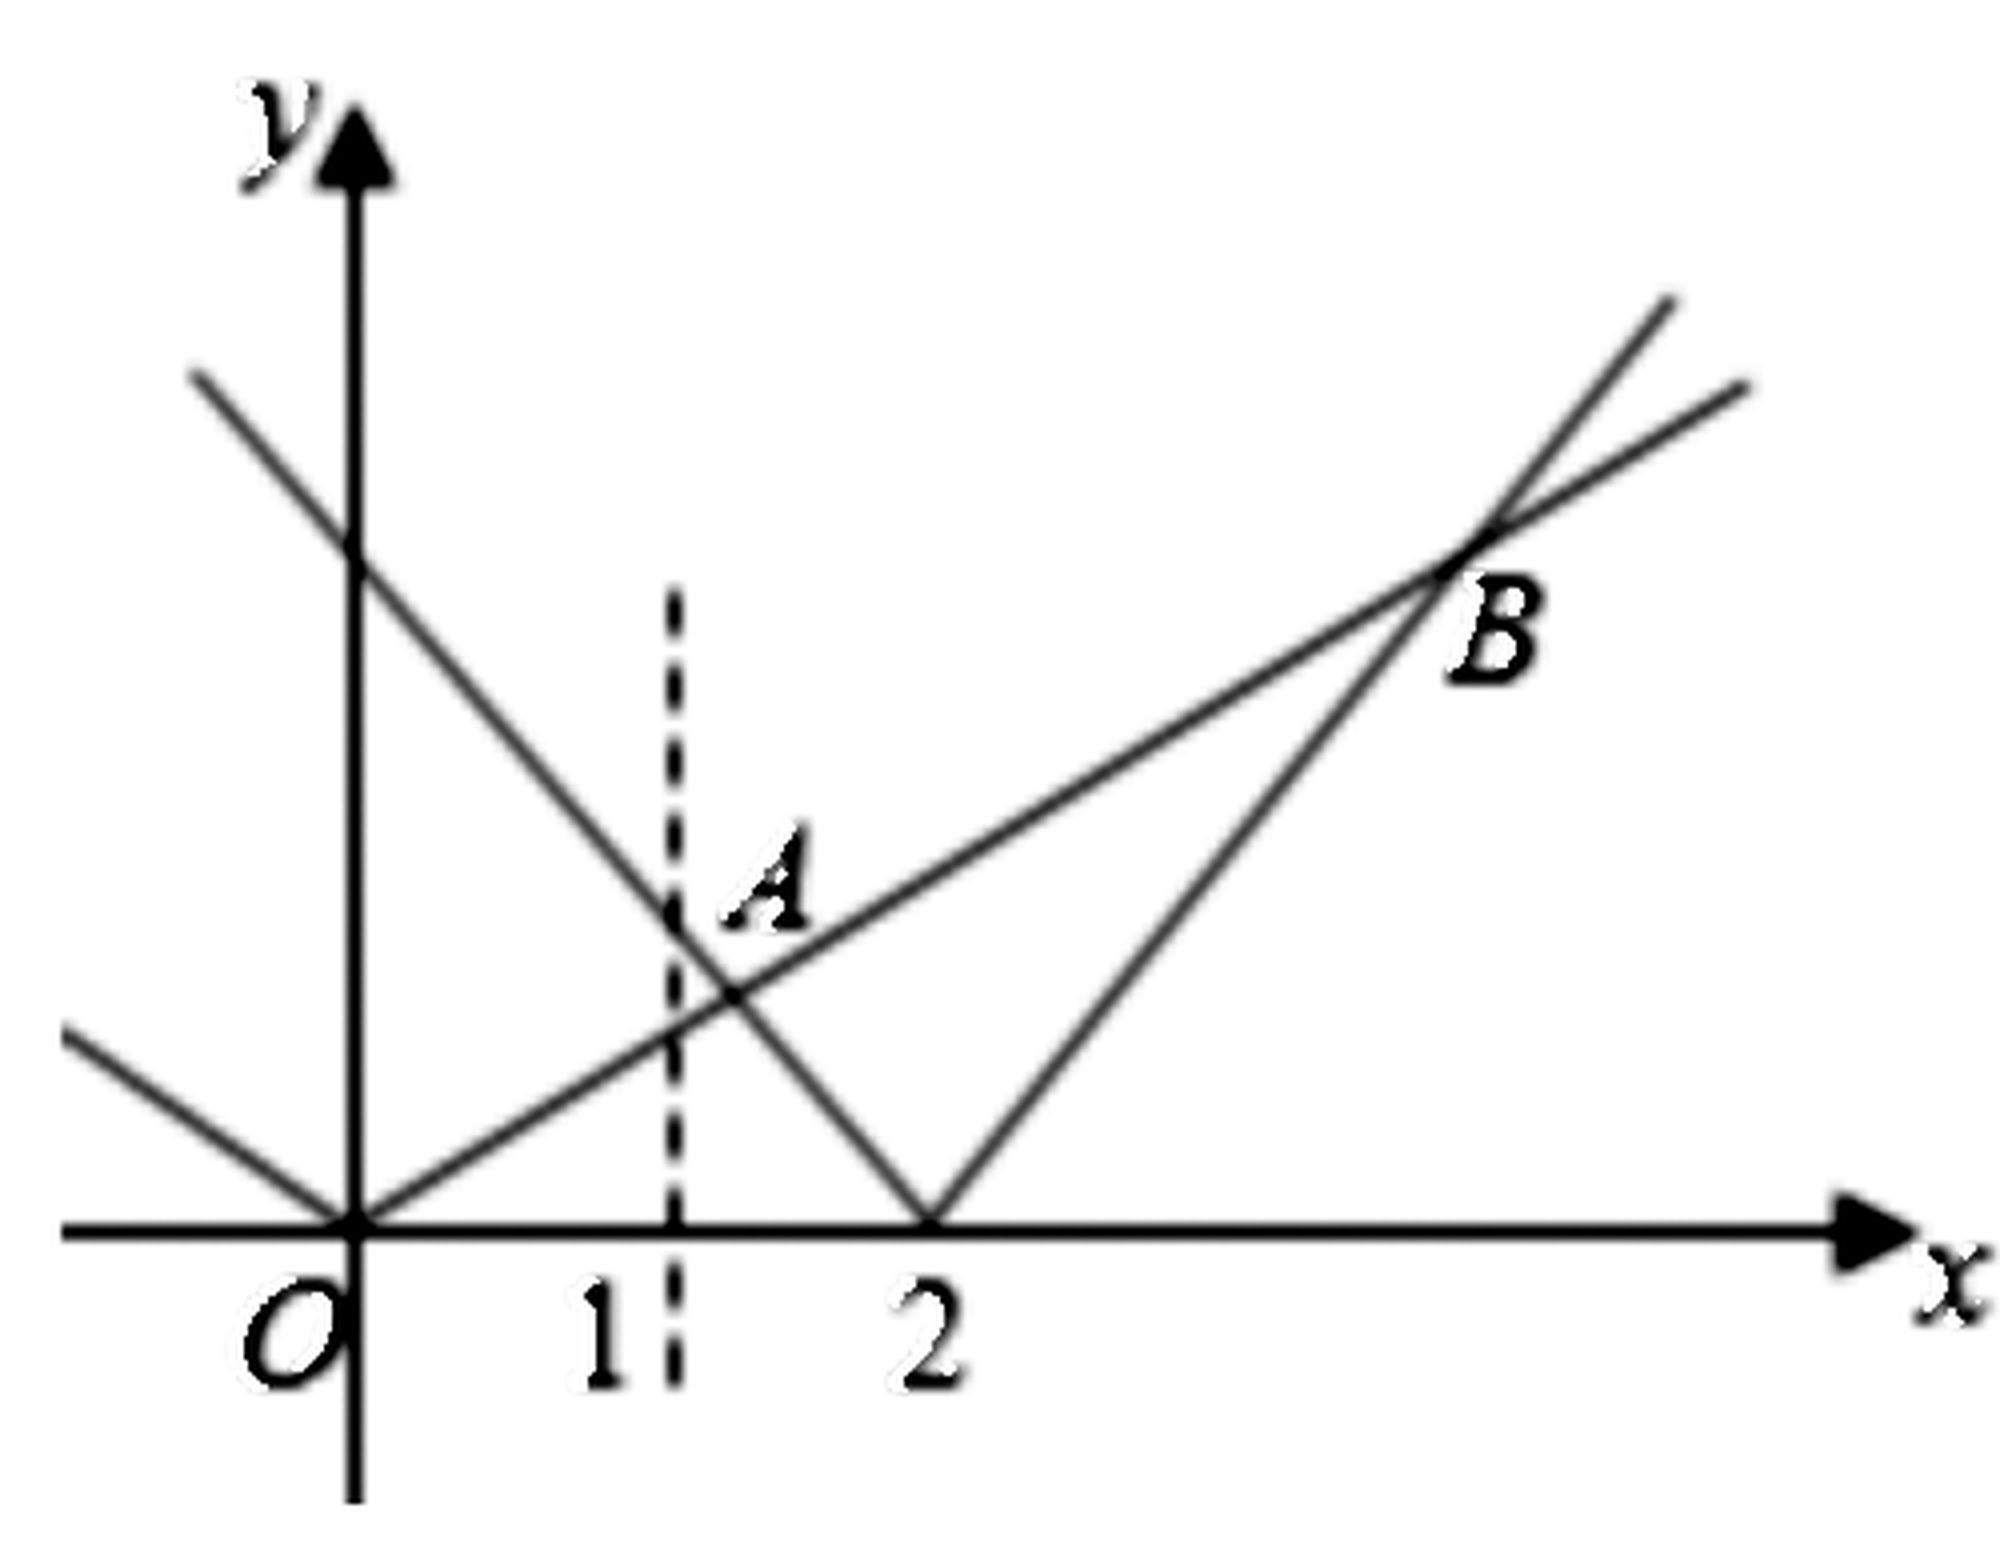
\includegraphics[width=0.40\textwidth]{figures/gao152_q15.png}
\end{center}
\step{由 $0<k<1$，得 $x_A>1$，}
\step{所以关于 $x$ 的不等式 $k\lvert x\rvert-\lvert x-2\rvert>0$ 恰好有 4 个整数解，是 2，3，4，5，}
\step{由 $\begin{cases}y=kx\\y=x-2\end{cases}\Rightarrow x_B=\dfrac2{1-k}\in(5,6]$，故 $\dfrac35<k\leqslant\dfrac23$；故选 $B$.}
\solend
\fi

% === Q16 === 咖啡优惠题；解析 12 行（跨 04 页上下半）；故选 C
\item 上海是全球咖啡店最多的城市. 若某品牌的某种在售咖啡产品价格为 30 元/杯，其原材料成本为 7 元/杯，营销成本为 5 元/杯，且该品牌门店提供如下 4 种优惠方式：(1) 首杯免单，每人限用一次；(2) 3.8 折优惠券，每人限用一次；(3) 买 2 杯送 2 杯，每人限用两次；(4) 买 5 杯送 5 杯，不限使用人数和使用次数. 每位消费者都可以在以上 4 种优惠方式中选择不多于 2 种使用. 现在某个公司有 5 位后勤工作人员去该品牌门店帮每位技术人员购买 1 杯咖啡，购买杯数与技术人员人数须保持一致；请问，这个公司的技术人员不少于\mbox{（\quad）}人时，无论 5 位后勤人员采用什么样的优惠方式购买咖啡，这笔订单该品牌门店都能保证盈利.

\keepwithprev
A. 20\qquad\qquad B. 25\qquad\qquad C. 30\qquad\qquad D. 35

\ifanswer
\solbegin
\step{按各优惠不叠加于同一杯理解，3.8 折券仅用于一杯，}
\step{买赠中的购买杯按原价付款.}
\step{设共购 $n$ 杯，免单、券购、原价购买的杯数分别为 $a,b,c$，其中 $0\leqslant a,b\leqslant5$，}
\step{其余为买赠咖啡，每杯成本为 12 元，}
\step{利润为 $P=15(n-a-b-c)+11.4b+30c-12n=3n-15a-3.6b+15c$，}
\step{若 $a,b$ 不同时为 5，则 $15a+3.6b\leqslant75+14.4=89.4$，}
\step{当 $n\geqslant30$ 时，$P\geqslant90-89.4=0.6>0$.}
\step{若 $a=b=5$，则每人均已使用免单和优惠券两种方式，其余均须原价购买，}
\step{$P=57+30(n-10)-12n=18n-243\geqslant297>0$.}
\step{当 $n=29$ 时，4 人各用方式 (1)(2) 购得 2 杯，}
\step{另 1 人用方式 (1) 及两次方式 (4) 购得 21 杯，}
\step{此时 $P=4\times11.4+2\times150-29\times12=-2.4<0$，因此最小人数为 30，故选 $C$.}% $2\times150$ 为两次方式（4）各买 5 杯的付款，照录（见 ⑤ 3）
\solend
\fi

\end{enumerate}

\bigsec{三、解答题}

\begin{enumerate}
\setcounter{enumi}{16}

% === Q17 === 解集含 \R／\varnothing；解析 4 行
\item 若 $a$、$b\in\R$，求关于 $x$ 的不等式 $ax\geqslant b$ 的解集.

\ifanswer
\solbegin
\step{当 $a>0$ 时，原不等式的解集为 $\left\{x\mid x\geqslant\dfrac ba\right\}$；}
\step{当 $a<0$ 时，原不等式的解集为 $\left\{x\mid x\leqslant\dfrac ba\right\}$；}
\step{当 $a=0$，$b\leqslant0$ 时，原不等式的解集为 $\R$；}
\step{当 $a=0$，$b>0$ 时，原不等式的解集为 $\varnothing$.}
\solend
\fi

% === Q18 === 子集 ⊆ 两处照录；cases 块；解析 9 行（跨 05 页上下半）
\item 已知 $\alpha:x<3m-1$ 或 $x>-m$，$\beta:x<2$ 或 $x\geqslant4$.

(1) 若 $\alpha$ 是 $\beta$ 的充分条件，求实数 $m$ 的取值范围；

(2) 若 $\alpha$ 是 $\beta$ 的必要条件，求实数 $m$ 的取值范围.

\ifanswer
\solbegin
\step{(1) 设 $A=\{x\mid x<3m-1\text{ 或 }x>-m\}$，$B=\{x\mid x<2\text{ 或 }x\geqslant4\}$，}
\step{因为 $\alpha$ 是 $\beta$ 的充分条件，所以 $A\subseteq B$，}
\step{当 $3m-1>-m$ 时，即 $m>\dfrac14$，此时 $A=\R$，不满足题意；}
\step{当 $3m-1\leqslant-m$ 时，即 $m\leqslant\dfrac14$，有 $\begin{cases}3m-1\leqslant2\\-m\geqslant4\end{cases}$，解得 $m\leqslant-4$；}
\step{综上，$m$ 的取值范围为 $(-\infty,-4]$.}
\step{(2) 因为 $\alpha$ 是 $\beta$ 的必要条件，所以 $B\subseteq A$，}
\step{当 $3m-1>-m$ 时，即 $m>\dfrac14$，此时 $A=\R$，$B\subseteq A$ 成立；}
\step{当 $3m-1\leqslant-m$ 时，即 $m\leqslant\dfrac14$，有 $\begin{cases}3m-1\geqslant2\\-m<4\end{cases}$，无解.}
\step{综上，$m$ 的取值范围为 $\left[\dfrac14,+\infty\right)$.}
\solend
\fi

% === Q19 === \varnothing 空集照录；解析 9 行
\item 设关于 $x$ 的不等式 $x^2+4x+k-1\geqslant0$ 的解集为 $A$.

(1) 若 $A=\R$，求实数 $k$ 的取值范围；

(2) 求证：不存在实数 $k$，使得 $A=\varnothing$.

\ifanswer
\solbegin
\step{(1) 配方得 $x^2+4x+k-1=(x+2)^2+k-5$，}
\step{若 $A=\R$，取 $x=-2$，得 $k-5\geqslant0$，即 $k\geqslant5$.}
\step{当 $k\geqslant5$ 时，对任意 $x\in\R$，都有 $(x+2)^2+k-5\geqslant0$，因此 $A=\R$.}
\step{所以 $k$ 的取值范围为 $[5,+\infty)$.}
\step{(2) 当 $k\geqslant5$ 时，由 (1) 得 $A=\R\ne\varnothing$.}
\step{当 $k<5$ 时，取 $x_0=-2+\sqrt{5-k}$，}
\step{则 $x_0^2+4x_0+k-1=(x_0+2)^2+k-5=(5-k)+k-5=0$，}
\step{所以 $x_0\in A$，即 $A\ne\varnothing$.}
\step{因此，不存在实数 $k$，使得 $A=\varnothing$.}
\solend
\fi

% === Q20 === |A\cap B|=1 印等号；等腰偏高粗 \Delta 照录；解析 12 行（跨 06→07 页）
\item 设 $m\in\R$. 集合 $A=\left\{x\mid\dfrac{x^2+x}{x+1}\geqslant\dfrac{2x+m}{x},x\in\R\right\}$，
$B=\left\{x\mid\dfrac{x^2+x}{x+1}\leqslant\dfrac{2x+m}{x},x\in\R\right\}$.

(1) 若 $m=8$，记集合 $M=A\cap(0,+\infty)$，求集合 $M$；

(2) 用 $\lvert T\rvert$ 代表集合 $T$ 的元素个数. 若 $\lvert A\cap B\rvert=1$，记 $m$ 的取值集合为 $C$，试比较 $\lvert C\rvert$ 与 2 的大小，并证明你的结论.

\ifanswer
\solbegin
\step{(1) 当 $m=8$，$x>0$ 时，$\dfrac{x^2+x}{x+1}\geqslant\dfrac{2x+8}{x}\Leftrightarrow x^2-2x-8\geqslant0$}
\step{$\Leftrightarrow(x-4)(x+2)\geqslant0\Leftrightarrow x\geqslant4$，所以 $M=[4,+\infty)$.}
\step{(2) 原分式有意义须 $x\ne-1,0$，因此 $x\in A\cap B\Leftrightarrow\begin{cases}x^2-2x-m=0\\x\ne-1,0\end{cases}$，}
\step{方程的判别式为 $\Delta=4(1+m)$.}
\step{当 $m<-1$ 时，方程无实根，$\lvert A\cap B\rvert=0$；}
\step{当 $m=-1$ 时，方程只有一个实根 1，$A\cap B=\{1\}$.}
\step{当 $m>-1$ 时，方程有两个不同实根.}
\step{其中，0 为根当且仅当 $m=0$，$-1$ 为根当且仅当 $m=3$.}
\step{$m=0$ 时，方程的根为 $0,2$，$A\cap B=\{2\}$；}
\step{$m=3$ 时，方程的根为 $-1,3$，$A\cap B=\{3\}$.}
\step{$m>-1$ 且 $m\ne0,3$ 时，两个实根均满足原分式的定义条件，$\lvert A\cap B\rvert=2$.}
\step{因此 $C=\{-1,0,3\}$，$\lvert C\rvert=3>2$.}
\solend
\fi

% === Q21 === "性质 p"新定义、\Q 归一、M\subseteq\R 照录；解析 19 行（跨 07→08 页）
\item 设集合 $M\subseteq\R$. 若 $M$ 中元素个数大于等于 2，且 $M$ 的任意不同元素 $a$、$b$ 均满足 $a^3-\dfrac14b\in M$，则称集合 $M$ 具有“性质 $p$”.

(1) 试判断集合 $\Q$、集合 $\left\{-\dfrac{\sqrt3}{2},0,\dfrac{\sqrt3}{2}\right\}$ 是否具有“性质 $p$”，并说明理由；

(2) 设 $m$ 为大于等于 2 的正整数. 若集合 $A=\{x_1,x_2,\cdots,x_m\}$，且具有“性质 $p$”，求证：$m=2$，并求集合 $A$ 中所有元素的乘积.

\ifanswer
\solbegin
\step{(1) $\Q$ 中至少有两个元素，且任意不同的 $a,b\in\Q$ 均满足 $a^3-\dfrac14b\in\Q$，}
\step{故 $\Q$ 具有“性质 $p$”.}
\step{对于另一集合，取 $a=0$，$b=\dfrac{\sqrt3}{2}$，则 $a^3-\dfrac14b=-\dfrac{\sqrt3}{8}$ 不属于该集合，}
\step{故其不具有“性质 $p$”.}
\step{(2) 将 $A$ 中元素按 $x_1<x_2<\cdots<x_m$ 排列.}
\step{若 $m\geqslant3$，由性质 $p$ 及幂函数 $y=x^3$ 的单调性，}
\step{有 $x_1^3-\dfrac14x_m<\cdots<x_1^3-\dfrac14x_2<x_m^3-\dfrac14x_2<x_m^3-\dfrac14x_1$，}
\step{上述 $m+1$ 个互不相同的数均属于 $A$，与 $A$ 只有 $m$ 个元素矛盾，}
\step{因此 $m=2$.}
\step{设 $A=\{a,b\}$，$a<b$.}
\step{因为 $a^3-\dfrac14b<b^3-\dfrac14a$，且两者均属于 $A$，}
\step{所以 $a^3-\dfrac14b=a$，$b^3-\dfrac14a=b$，}
\step{两式相减并除以 $a-b\ne0$，}
\step{以及两式相加，分别得 $a^2+ab+b^2=\dfrac34$，$(a+b)(a^2-ab+b^2)=\dfrac54(a+b)$，}
\step{代入 $a^2-ab+b^2=\dfrac34-2ab$，得 $(a+b)(4ab+1)=0$，}
\step{若 $a+b=0$，则 $-ab=a^2+ab+b^2=\dfrac34$，即 $ab=-\dfrac34$；}
\step{若 $a+b\ne0$，则 $ab=-\dfrac14$.}
\step{分别取 $A=\left\{-\dfrac{\sqrt3}{2},\dfrac{\sqrt3}{2}\right\}$，$A=\left\{\dfrac{1-\sqrt3}{2\sqrt2},\dfrac{1+\sqrt3}{2\sqrt2}\right\}$，}
\step{代入均有 $a^3-\dfrac14b=a$、$b^3-\dfrac14a=b$，故两种乘积均可取得.}
\solend
\fi

\end{enumerate}

\end{document}
"
% 紧凑版：xelatex "\def\iscompact{1}% 高一152_位育中学_期中.tex
%   —— 高一上数学"2026-2027 年位育中学高一上期中"（试卷版/答案版/紧凑版）
% 试卷版：xelatex 高一152_位育中学_期中.tex
% 答案版：xelatex "\def\isanswer{1}% 高一152_位育中学_期中.tex
%   —— 高一上数学"2026-2027 年位育中学高一上期中"（试卷版/答案版/紧凑版）
% 试卷版：xelatex 高一152_位育中学_期中.tex
% 答案版：xelatex "\def\isanswer{1}\input{高一152_位育中学_期中.tex}"
% 紧凑版：xelatex "\def\iscompact{1}\input{高一152_位育中学_期中.tex}"
%
% ① 原始材料：微信公众号"魔都数学加油站"文章，连载"27学年高一152"，原文标题
% "27学年高一152——2026-2027年上海市位育中学高一上期中"；
% 原文链接：https://mp.weixin.qq.com/s/v4_G6oTX2BuPz9L-KtLRfw 。
% 正文为 8 张 PNG 页（01/03/05/06/07/08 为 2560×3620，02/04 为 4762×6735，
% 同一篇各页分辨率混排，逐页按各自分辨率裁图核对，别按预览比例换算裁框）。
% 体例：讲评版——填空 3—12（10 题）、选择 13—16（4 题）、解答 17—21（5 题），
% 共 19 题，自第 3 题起编；题目、答案、解析均据原图转录；卷面粉红色水印
% "魔都数学加油站"及公众号页脚未录入。
% 全卷插图清单（逐页通读 8 页确认）：1 幅——第 15 题解析配图（两条折线
% $y=k\lvert x\rvert$ 与 $y=\lvert x-2\rvert$ 及坐标图，03 页右下，含 O、1、2、
% A、B 与虚线 $x=1$），解析写"的图象如下"，仅答案版出，裁
% figures/gao152_q15.png（去粉水印、去色、4× LANCZOS 放大）。
%
% 卷首标题：原卷印作"2026-2027 年位育中学高一上期中"，年份区间按全稿惯例排 en dash；
% 原卷卷面未印副标题，本稿按同期中卷知识模块口径补出"集合与常用逻辑用语、不等式、函数"。
%
% ② 与原卷的排版差异：
%   ① 原文从第 3 题起，本稿保留原题号；共 19 题三节，解答题 5 题到 21；
%   ② 混合体例：第 3、5 题只印【答案】、无【解析】，按 高一140 第 5 题／
%      高一145 第 3 题成例另提 \ans{}、不补造解析；第 13、14 题把答案"D"
%      直接印在题干括号内、题下无【解析】，按 高一84／148／149 成例括号留空、
%      另提 \ans{$D$}；其余 15 题印【解析】、用 \solbegin…\solend；
%      第 15、16 题答案在解析末句"故选 B／C"、括号留空、不另提 \ans{}；
%      答案版【答案】/【解析】标记数 = 19 = 全卷题数（4 个 \ans ＋ 15 个 \solbegin）；
%   ③ 原卷卷面未印副标题，本稿按知识模块口径补出；
%   ④ 原卷填空横线按全稿惯例排 \blankline[4.4em]；选择题括号排 \mbox{（\quad）}、
%      四道选择题的选项段前按惯例各加 \keepwithprev；解答题不留作答区、不加
%      \anspace（原卷为讲评版，109—113 起全稿不用 \anspace）；
%   ⑤ 数集黑板粗体：Q7"全集为 R"、Q9"$\lVert PQ\rVert$ 定义"无数集、
%      Q12"$t\in Z$"、Q13"$k\in Z$ 与 $=\R$"、Q17"$a,b\in R$"、Q19"$A=\R$"、
%      Q20"$m\in\R$"、Q21"$M\subseteq\R$ 与集合 $\Q$"原卷印正体粗体或黑板体
%      R/Q/Z，按全稿惯例归一 \R／\Q／\Z；绝对值排 \lvert…\rvert
%      （Q4、Q9、Q11、Q15），集合描述竖线排 \mid（Q7、Q13、Q20、Q21），
%      距离双竖线排 \lVert…\rVert（Q9 与题干、解析的 ||PQ||／||AB||）；
%      不等号按全稿惯例排 \leqslant／\geqslant；补集照原卷上划线排 \overline{A}
%      （Q7 题干＋解析）；空集 \varnothing（Q17、Q19）；
%      子集 Q18 两处、Q21 题干一处均印带下划线 ⊆、照录 \subseteq（见 ④），
%      本卷无单线 \subset 用例；
%   ⑥ 判别式 Δ/△ 两形混用逐处照录、不得统一：Q11 解析"判别式 △=k²−8k>0"
%      印扁等边细线三角、照录 \triangle，Q20 (2) 解析"判别式为 Δ=4(1+m)"
%      印等腰偏高粗三角、照录 \Delta（/tmp/gao152/z/zoom/q11_delta.png、
%      q20_delta.png 放大并与 151 卷同型并排比较）；
%   ⑦ 中文弯引号照录：Q11"长度"、Q21"性质 p"（题干、两问与解析多处）、
%      Q6 从">"、"<"、"≥"、"≤"中选符号、Q16"（1）…（4）"半角括号；
%      注释里一律 ASCII 引号；数学式内 CJK 用 \text{}（Q13 的"或／且"、
%      Q18 集合描述的"或"）；
%   ⑧ "图像／图象"：全卷仅 Q15 解析一处"的图象如下"，印"图象"（象，无亻）、
%      照录；其余各题无"图像"字样。子题标号 (1)(2)(3)(4) 半角括号照录；
%   ⑨ 半角逗号在数学组之间是全稿惯例、非笔误，逐处照录（Q6、Q10、Q16、
%      Q20、Q21 的 $a,b,c$ 之类）；行末西文句点 ASCII `.`；
%      行中全角逗号／顿号照录（Q11"（a,b）"、Q16"7 元/杯"、Q21"$\Q$、集合"）；
%   ⑩ 复杂式照录别简化：Q4 四组 cases 块（整体各占一个印刷行）、Q8
%      $\frac{x_0}{e^{x_0}}=\frac13$、Q10 $4a^2+b^2=4$、Q12 $b=\frac2a$、
%      Q16 利润式 $P=15(n-a-b-c)+11.4b+30c-12n$、Q18 cases 块、
%      Q20 分式 $\frac{x^2+x}{x+1}$、Q21 $a^3-\frac14b$ 与两组取值集合；
%      \left…\right 不得拆到不同 $…$ 组（Q4 cases 前的 \left\{ 一律改
%      \begin{cases}…\end{cases}、Q17 $\left\{x\mid x\ge\frac ba\right\}$、
%      Q20 $\left\{x\mid\cdots\right\}$、Q21 $\left\{-\frac{\sqrt3}2,\ldots\right\}$）；
%   ⑪ 一条 \step = 原卷解析的一个印刷行，cases 块整体算一个印刷行；别并折行、
%      别拆行。Q12 七行、Q16 十二行、Q18 九行、Q19 九行、Q20 十二行、
%      Q21 十九行均按印刷行逐条断，不丢行；
%   ⑫ 配图：Q15 解析配图（仅答案版出）放 \ifanswer 内 \solbegin…\solend 的
%      \step 之间（高一73 第 16 题／高一150 Q12 成例）；题干无配图，故无
%      \needvspace；
%   ⑬ 原卷解析内无红色"法一／法二"之类小标题，故本卷无 \stepm；红色水印
%      "魔都数学加油站"不录入；
%   ⑭ 跨页续印按题合并：见 ⑥；
%
% ③ 行数复核：一条 \step = 原卷解析的一个印刷行，cases 块作一个印刷行计。
%   逐题数（主会话逐页核对定稿）：Q3：0（只印【答案】、提 \ans{}）；Q4：2；
%   Q5：0（只印【答案】、提 \ans{}）；Q6：1；Q7：1；Q8：1；Q9：1；
%   Q10：4；Q11：5；Q12：7；Q13：0（答案印括号内、提 \ans{}）；
%   Q14：0（答案印括号内、提 \ans{}）；Q15：4；Q16：12；Q17：4；
%   Q18：9；Q19：9；Q20：12；Q21：19。
%   合计 91 条 \step（本卷无 \stepm），与原卷逐题印刷行相等。全卷 15 题设
%   \solbegin…\solend ＋ Q3／Q5／Q13／Q14 四处 \ans{}，答案版
%   【答案】/【解析】标记数 = 19 = 全卷题数。
%
% ④ 判别式／子集符号结论（逐处放大原图照录、不得统一，主会话像素级复核）：
%   判别式：Q11 解析"方程 $x^2-kx+2k=0$ 的判别式 $\triangle=k^2-8k>0$"
%      印扁等边细线三角、照录 \triangle；Q20 (2) 解析"方程的判别式为
%      $\Delta=4(1+m)$"印等腰偏高粗三角、照录 \Delta
%      （/tmp/gao152/z/zoom/q11_delta.png、q20_delta.png；与 高一142／151
%      的"Δ/△ 混用逐处照录"口径一致）。本卷无几何三角形符号。
%   子集：Q18 解析 (1)"$A\subseteq B$"、(2)"$B\subseteq A$"与 Q21 题干
%      "$M\subseteq\R$"共 3 处均印带下划线 ⊆、照录 \subseteq
%      （/tmp/gao152/z/zoom/q18_subset.png、q21_subset.png 放大确认）；
%      本卷无单线 ⊂ 用例。补集上划线 \overline{A}（Q7）、空集 \varnothing
%      （Q17 解析末行、Q19 题干 (2) 与解析）、数集 \R／\Q／\Z 归一见 ② ⑤。
%
% ⑤ 存疑照录（放大原图确认，照录未改、正文对应处另有 % 注）：
%   1. Q11 题干"已知关于 $x$ 的不等式 $x^2-kx+2k<0$ 有实数解，且解集区间
%      长度不超过 3 个单位"，解析据 $\lvert x_1-x_2\rvert\leqslant3$ 推；
%      判别式用扁三角 \triangle（见 ④），照录未改。
%   2. Q12 解析"$t=-1$ 时取 $b=\frac2a\in[-2,-1]$，$c=-1$，则 $ab+c=2-1=1$"
%      ——$b$ 径写 $\frac2a$（无负号），放大 03 页确认，照录未改。
%   3. Q16 解析"$P=4\times11.4+2\times150-29\times12=-2.4<0$"中的
%      $2\times150$ 为两次方式（4）各买 5 杯的付款，照录未改。
%   4. Q20 (2) 题干"若 $\lvert A\cap B\rvert=1$"印等号（非 $\leqslant1$），
%      放大 06 页 /tmp/gao152/z/zoom/q20_eq1.png 确认，照录未改。
%   5. Q21 题干"性质 p"用弯引号且 $p$ 为斜体小写，逐处照录未统一；
%      解析 (2) 末两组 $A$ 的取值集合照录未简化。
%   6. "图像／图象"仅 Q15 一处"图象"、Δ/△ 两形并用（Q11 \triangle、
%      Q20 \Delta）均逐处照录、未统一（见 ② ⑥ ⑧ 与 ④）。
%   全卷除此 6 类外未发现其它笔误／自相矛盾处；19 题中 15 题印【解析】、
%   Q3／Q5 只印【答案】、Q13／Q14 答案印题干括号内（见 ② ②）。
%
% ⑥ 跨页续印按题合并说明（逐页核实定稿）：Q3—Q5 题干＋【答案】／【解析】
%   在 01 页上半，Q6—Q8 题干＋解析在 01 页下半；Q9、Q10 题干＋解析、
%   Q11 题干＋解析、Q12 题干＋解析首行在 02 页；Q12 解析余 6 行续 03 页
%   上半，"二、选择题"标题与 Q13 题干＋选项在 03 页下半；Q13 选项 C／D、
%   Q14 题干＋四选项＋（无解析）、Q15 题干＋四选项＋解析前 3 行＋配图在
%   03 页下半，Q15 解析末行（由 cases 求 $x_B$）续 04 页顶；Q16 题干＋四选项
%   ＋解析前 5 行在 04 页上半，解析余 7 行在 04 页下半；"三、解答题"标题与
%   Q17 题干＋解析首行在 04 页末，Q17 解析余 3 行、Q18 题干＋两问＋解析首
%   4 行在 05 页上半，Q18 解析余 5 行在 05 页下半；Q19 题干＋两问＋解析
%   (1) 4 行在 05—06 页（(2) 题干续 06 页顶），解析 (2) 5 行在 06 页上半；
%   Q20 题干＋两问＋解析 (1) 2 行＋(2) 首行在 06 页下半；Q20 (2) 解析余
%   9 行、Q21 题干＋两问＋解析 (1) 4 行在 07 页；Q21 (2) 解析 19 行中前
%   6 行在 07—08 页上半、末 13 行续 08 页下半，末行"故两种乘积均可取得"
%   为全卷收尾（08 页下半仅水印、无其它正文）。
%   本稿按题连排，不丢行、不并折行；全卷末题为第 21 题，无附加题节。
%
\documentclass[a4paper,11pt]{article}
\usepackage{common}

\begin{document}

\examtitlest[3]{2026--2027 年位育中学高一上期中}{集合与常用逻辑用语、不等式、函数}

\bigsec{一、填空题}

\begin{enumerate}
\setcounter{enumi}{2}

% === Q3 === 原卷只印【答案】、无【解析】，另提 \ans{}，不补造解析
\item 设 $x>0$. 若 $\ln x=-1$，则 $x=$\blankline[4.4em].

\ifanswer
\ans{$\dfrac1{\mathrm{e}}$}
\fi

% === Q4 === 四组 cases 块同一印刷行；解析 2 行
\item 不等式 $\lvert 1-2x\rvert>x$ 的解集为\blankline[4.4em].

\ifanswer
\solbegin
\step{不等式 $\lvert 1-2x\rvert>x$ 即为 $\begin{cases}1-2x\geqslant0\\1-2x>x\end{cases}$ 或 $\begin{cases}1-2x<0\\2x-1>x\end{cases}$，即 $\begin{cases}x\leqslant\frac12\\x<\frac13\end{cases}$ 或 $\begin{cases}x>\frac12\\x>1\end{cases}$，}
\step{则有 $x<\dfrac13$ 或 $x>1$，则解集为 $\left(-\infty,\dfrac13\right)\cup(1,+\infty)$.}
\solend
\fi

% === Q5 === 原卷只印【答案】、无【解析】；\frac1x\ge1 印单线 ≥，按全稿惯例 \geqslant
\item 不等式 $\dfrac1x\geqslant1$ 的解集为\blankline[4.4em].

\ifanswer
\ans{$(0,1]$}
\fi

% === Q6 === 从四个符号中选一个，中文弯引号照录；解析 1 行
\item 设 $a$、$b>0$，则 $a^2+b^2$\blankline[4.4em]$2(2a-b)-5$（从“$>$”、“$<$”、“$\geqslant$”、“$\leqslant$”中选择一个符号填写）.

\ifanswer
\solbegin
\step{$a^2+b^2-[2(2a-b)-5]=(a-2)^2+(b+1)^2>0$，故 $a^2+b^2>2(2a-b)-5$.}
\solend
\fi

% === Q7 === 补集上划线 \overline{A}；集合描述竖线 \mid；解析 1 行
\item 已知全集为 $\R$，集合 $A=\{x\mid y=\sqrt{x-2}\}$，集合 $B=\{y\mid y=\sqrt{x-2}\}$，则 $\overline{A}\cap B=$\blankline[4.4em].

\ifanswer
\solbegin
\step{$A=[2,+\infty)$，$B=[0,+\infty)$，所以 $\overline{A}\cap B=[0,2)$.}
\solend
\fi

% === Q8 === \frac{x_0}{e^{x_0}}=\frac13 照录；解析 1 行
\item 设正数 $x_0$ 满足等式 $\dfrac{x_0}{e^{x_0}}=\dfrac13$，则 $x_0-\ln x_0=$\blankline[4.4em].

\ifanswer
\solbegin
\step{等式两边取自然对数，得 $\ln x_0-x_0=-\ln3$，即 $x_0-\ln x_0=\ln3$.}
\solend
\fi

% === Q9 === 距离双竖线 \lVert…\rVert；解析 1 行
\item 在平面直角坐标系 $xOy$ 中，设点 $P(x_1,y_1)$，$Q(x_2,y_2)$，定义：$\lVert PQ\rVert=\lvert x_1-x_2\rvert+\lvert y_1-y_2\rvert$. 若点 $A(1,0)$，点 $B$ 为直线 $y=x+2$ 上的动点，则 $\lVert AB\rVert$ 的最小值为\blankline[4.4em].

\ifanswer
\solbegin
\step{$\lVert AB\rVert=\lvert x-1\rvert+\lvert y\rvert=\lvert x-1\rvert+\lvert x+2\rvert\geqslant3$，最小值为 3.}
\solend
\fi

% === Q10 === 解析 4 行
\item 已知 $a$、$b$ 均为正数，且 $a^2+\dfrac14b^2=1$，则 $a\sqrt{1+b^2}$ 的最大值为\blankline[4.4em].

\ifanswer
\solbegin
\step{因为 $a$、$b$ 均为正数，且 $a^2+\dfrac14b^2=1$，所以 $4a^2+b^2=4$，}
\step{所以 $a\sqrt{1+b^2}=\dfrac12\cdot2a\cdot\sqrt{1+b^2}\leqslant\dfrac12\cdot\dfrac{4a^2+1+b^2}{2}=\dfrac54$，}
\step{当且仅当 $4a^2=b^2+1$ 即 $a=\dfrac{\sqrt{10}}4$，$b=\dfrac{\sqrt6}2$ 时取等号，}
\step{故 $a\sqrt{1+b^2}$ 的最大值为 $\dfrac54$.}
\solend
\fi

% === Q11 === 扁等边细线判别式 \triangle 照录（见 ④）；"长度"弯引号；解析 5 行
\item 一般地，把 $b-a$ 称为区间 $(a,b)$ 的“长度”. 已知关于 $x$ 的不等式 $x^2-kx+2k<0$ 有实数解，且解集区间长度不超过 3 个单位，则实数 $k$ 的取值范围是\blankline[4.4em].

\ifanswer
\solbegin
\step{因为不等式 $x^2-kx+2k<0$ 有解，}
\step{所以方程 $x^2-kx+2k=0$ 的判别式 $\triangle=k^2-8k>0$，解得 $k>8$ 或 $k<0$，}
\step{由 $x_1+x_2=k$，$x_1x_2=2k$，得 $(x_1-x_2)^2=(x_1+x_2)^2-4x_1x_2=k^2-8k$，}
\step{由 $\lvert x_1-x_2\rvert\leqslant3$，得 $(x_1-x_2)^2\leqslant9$，即 $k^2-8k\leqslant9$，解得 $-1\leqslant k\leqslant9$，}
\step{所以 $-1\leqslant k<0$ 或 $8<k\leqslant9$，即实数 $k$ 的取值范围是 $[-1,0)\cup(8,9]$.}
\solend
\fi

% === Q12 === $b=\frac2a$ 无负号、$c=-1$ 照录（见 ⑤ 2）；解析 7 行（跨 02→03 页）
\item 设 $t\in\Z$，且对任意 $a\in[-2,t]$，总存在 $b,c\in[-2,t]$，使得 $ab+c=1$，则 $t$ 的所有取值为\blankline[4.4em].

\ifanswer
\solbegin
\step{$[-2,t]$ 是区间，要求 $t>-2$，故 $t\geqslant-1$.}
\step{当 $t\geqslant1$ 时，对任意 $a\in[-2,t]$，}
\step{取 $b=0$，$c=1$，两者都属于 $[-2,t]$，且 $ab+c=1$.}
\step{当 $t=0$ 时，取 $a=0$，则 $c=1\notin[-2,0]$，不成立.}
\step{当 $t=-1$ 时，对任意 $a\in[-2,-1]$，取 $b=\dfrac2a\in[-2,-1]$，$c=-1$，}% 原卷径写 $b=\frac2a$（无负号），放大 03 页确认，照录未改（见 ⑤ 2）
\step{则 $ab+c=2-1=1$.}
\step{所以 $t=-1$ 或 $t\geqslant1$（$t\in\Z$）.}
\solend
\fi

\end{enumerate}

\bigsec{二、选择题}

\begin{enumerate}
\setcounter{enumi}{12}

% === Q13 === 答案 D 印在题干括号内、无【解析】，按 高一84／148／149 成例括号留空、另提 \ans{}
\item 下列说法错误的是\mbox{（\quad）}

\keepwithprev
A. 奇数集可以表示为 $\{x\mid x=2k+1,k\in\Z\}$

B. 奇数集可以表示为 $\{x\mid x=2k-1,k\in\Z\}$

C. $\{x\mid x\ne2\text{ 或 }x\ne-2\}=\R$

D. $\{x\mid x\ne2\text{ 且 }x\ne-2\}=\R$

\ifanswer
\ans{$D$}
\fi

% === Q14 === 答案 D 印在题干括号内、无【解析】；选项两行两列
\item 设 $a$、$b$、$c>0$，且 $a\ne1$，则以下代数式中，不恒成立的是\mbox{（\quad）}

\keepwithprev
A. $\log_a 1=0$\qquad\qquad B. $a^{\log_a b}=b$

C. $\log_a b+\log_a c=\log_a(bc)$\qquad\qquad D. $\log_a b=\dfrac1{\log_b a}$

\ifanswer
\ans{$D$}
\fi

% === Q15 === "图象"（象，无亻）照录；解析配图仅答案版出；答案在解析末句故选 B
\item 若关于 $x$ 的不等式 $k\lvert x\rvert>\lvert x-2\rvert$ 恰好有 4 个整数解，则实数 $k$ 的取值范围是\mbox{（\quad）}

\keepwithprev
A. $\left(\dfrac35,\dfrac23\right)$\qquad B. $\left(\dfrac35,\dfrac23\right]$\qquad C. $\left(\dfrac35,1\right)$\qquad D. $\left(\dfrac35,1\right]$

\ifanswer
\solbegin
\step{由题意得 $0<k<1$，函数 $y=k\lvert x\rvert$ 与 $y=\lvert x-2\rvert$ 的图象如下，}
\begin{center}
% 两条折线坐标图取 03 页右下，去粉色水印、去色、4× LANCZOS 放大；仅答案版出
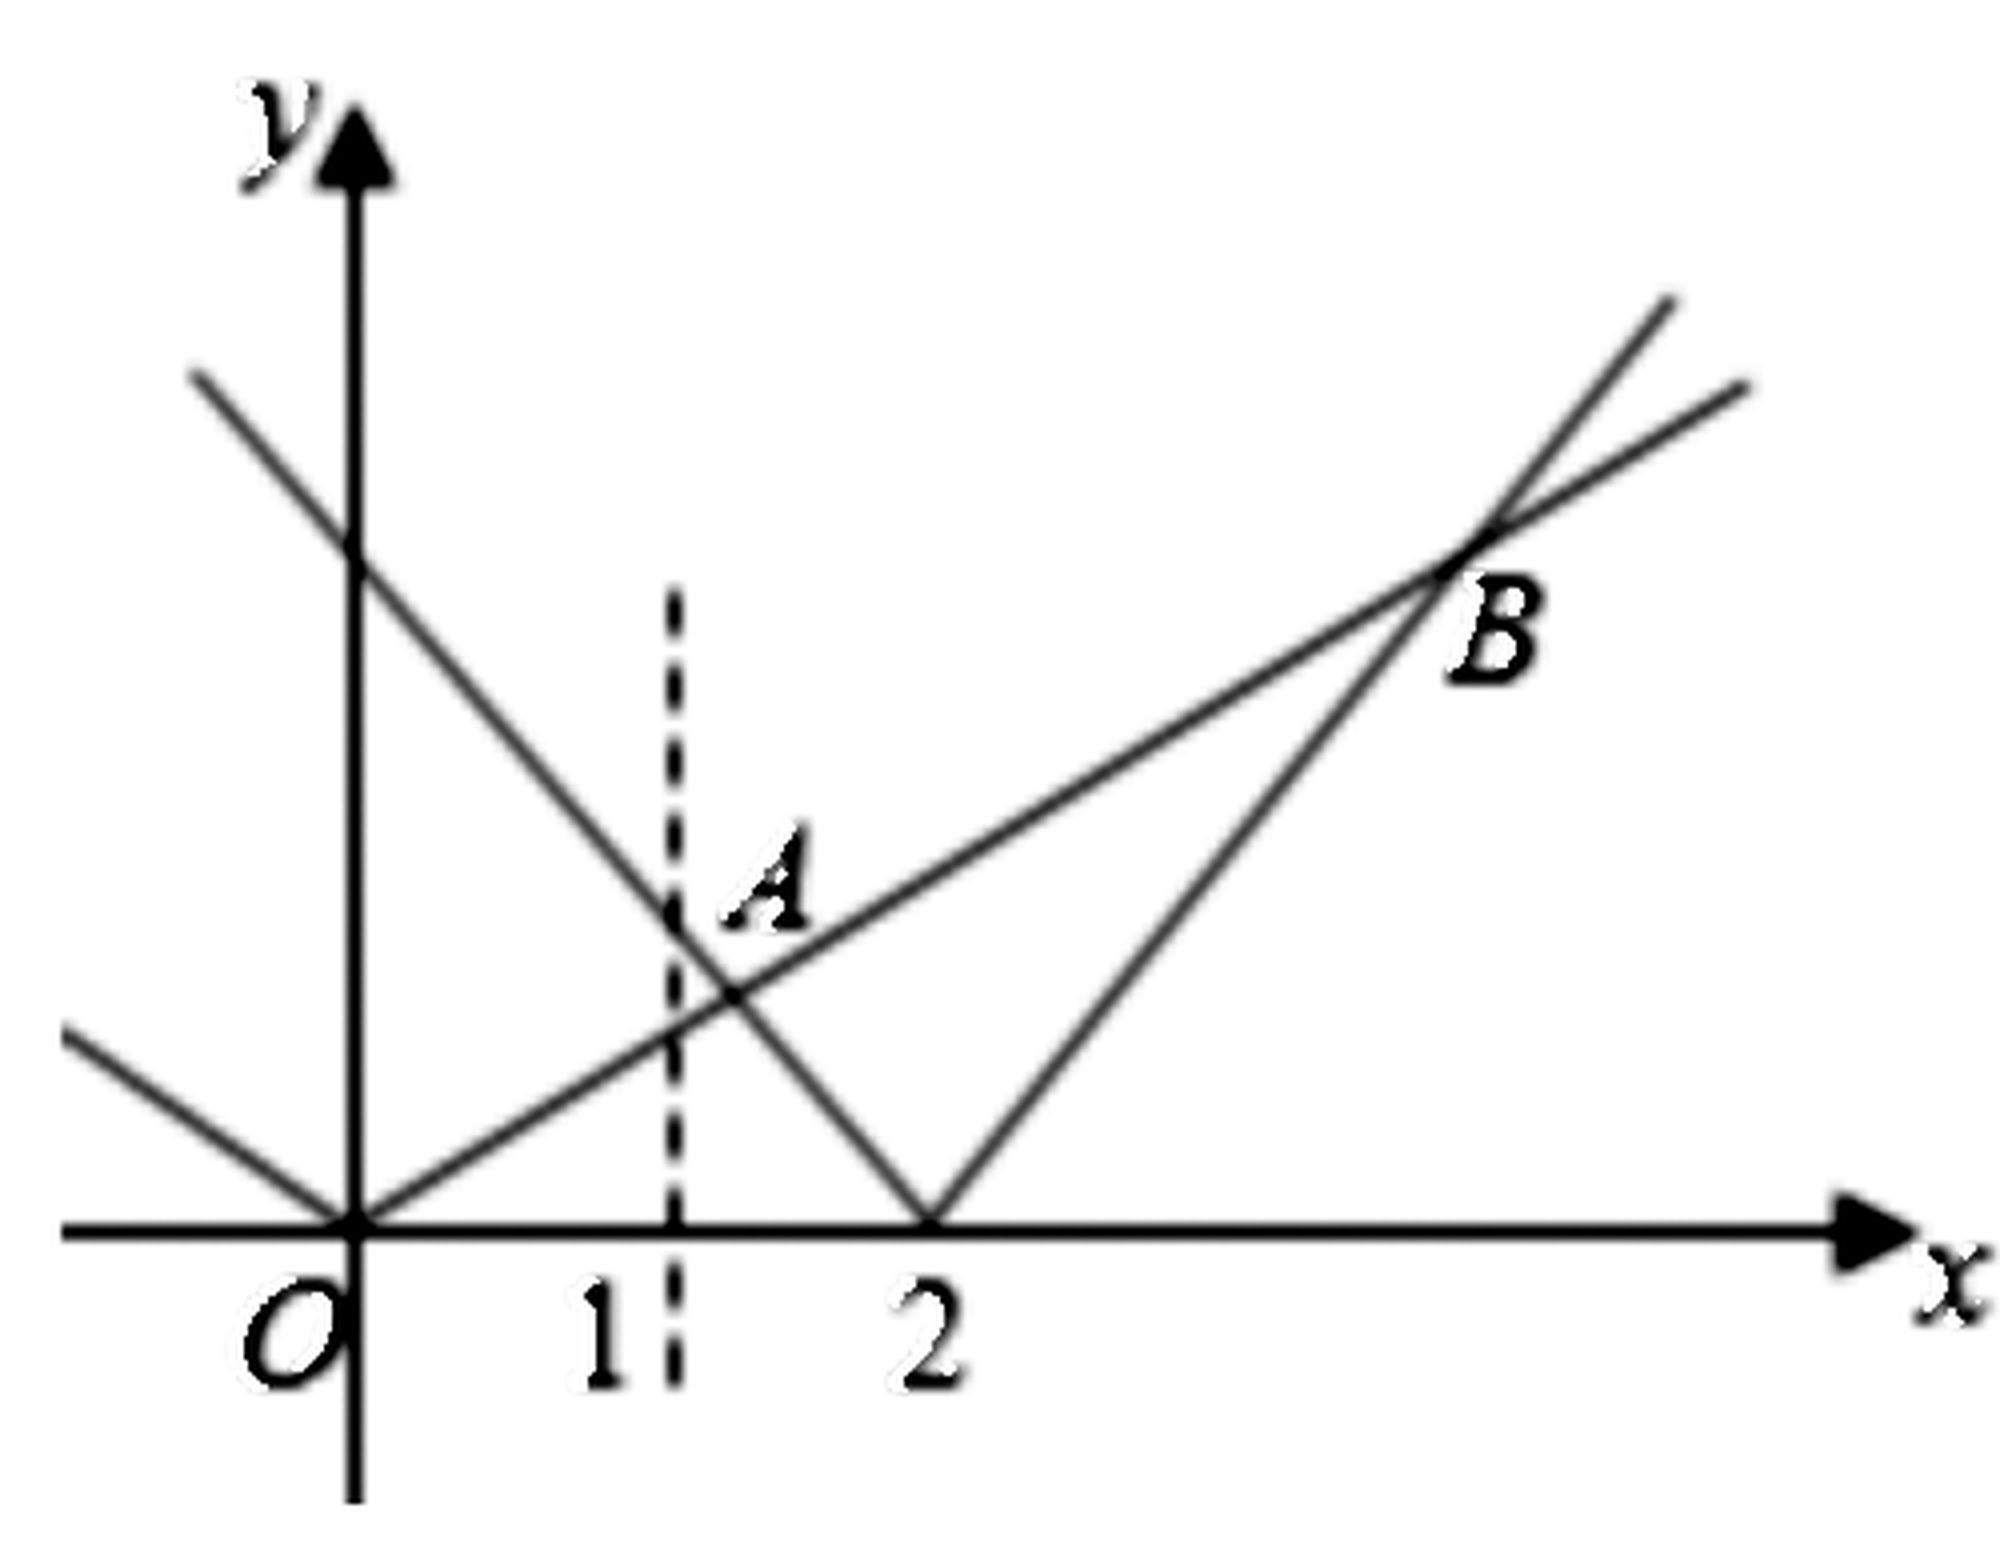
\includegraphics[width=0.40\textwidth]{figures/gao152_q15.png}
\end{center}
\step{由 $0<k<1$，得 $x_A>1$，}
\step{所以关于 $x$ 的不等式 $k\lvert x\rvert-\lvert x-2\rvert>0$ 恰好有 4 个整数解，是 2，3，4，5，}
\step{由 $\begin{cases}y=kx\\y=x-2\end{cases}\Rightarrow x_B=\dfrac2{1-k}\in(5,6]$，故 $\dfrac35<k\leqslant\dfrac23$；故选 $B$.}
\solend
\fi

% === Q16 === 咖啡优惠题；解析 12 行（跨 04 页上下半）；故选 C
\item 上海是全球咖啡店最多的城市. 若某品牌的某种在售咖啡产品价格为 30 元/杯，其原材料成本为 7 元/杯，营销成本为 5 元/杯，且该品牌门店提供如下 4 种优惠方式：(1) 首杯免单，每人限用一次；(2) 3.8 折优惠券，每人限用一次；(3) 买 2 杯送 2 杯，每人限用两次；(4) 买 5 杯送 5 杯，不限使用人数和使用次数. 每位消费者都可以在以上 4 种优惠方式中选择不多于 2 种使用. 现在某个公司有 5 位后勤工作人员去该品牌门店帮每位技术人员购买 1 杯咖啡，购买杯数与技术人员人数须保持一致；请问，这个公司的技术人员不少于\mbox{（\quad）}人时，无论 5 位后勤人员采用什么样的优惠方式购买咖啡，这笔订单该品牌门店都能保证盈利.

\keepwithprev
A. 20\qquad\qquad B. 25\qquad\qquad C. 30\qquad\qquad D. 35

\ifanswer
\solbegin
\step{按各优惠不叠加于同一杯理解，3.8 折券仅用于一杯，}
\step{买赠中的购买杯按原价付款.}
\step{设共购 $n$ 杯，免单、券购、原价购买的杯数分别为 $a,b,c$，其中 $0\leqslant a,b\leqslant5$，}
\step{其余为买赠咖啡，每杯成本为 12 元，}
\step{利润为 $P=15(n-a-b-c)+11.4b+30c-12n=3n-15a-3.6b+15c$，}
\step{若 $a,b$ 不同时为 5，则 $15a+3.6b\leqslant75+14.4=89.4$，}
\step{当 $n\geqslant30$ 时，$P\geqslant90-89.4=0.6>0$.}
\step{若 $a=b=5$，则每人均已使用免单和优惠券两种方式，其余均须原价购买，}
\step{$P=57+30(n-10)-12n=18n-243\geqslant297>0$.}
\step{当 $n=29$ 时，4 人各用方式 (1)(2) 购得 2 杯，}
\step{另 1 人用方式 (1) 及两次方式 (4) 购得 21 杯，}
\step{此时 $P=4\times11.4+2\times150-29\times12=-2.4<0$，因此最小人数为 30，故选 $C$.}% $2\times150$ 为两次方式（4）各买 5 杯的付款，照录（见 ⑤ 3）
\solend
\fi

\end{enumerate}

\bigsec{三、解答题}

\begin{enumerate}
\setcounter{enumi}{16}

% === Q17 === 解集含 \R／\varnothing；解析 4 行
\item 若 $a$、$b\in\R$，求关于 $x$ 的不等式 $ax\geqslant b$ 的解集.

\ifanswer
\solbegin
\step{当 $a>0$ 时，原不等式的解集为 $\left\{x\mid x\geqslant\dfrac ba\right\}$；}
\step{当 $a<0$ 时，原不等式的解集为 $\left\{x\mid x\leqslant\dfrac ba\right\}$；}
\step{当 $a=0$，$b\leqslant0$ 时，原不等式的解集为 $\R$；}
\step{当 $a=0$，$b>0$ 时，原不等式的解集为 $\varnothing$.}
\solend
\fi

% === Q18 === 子集 ⊆ 两处照录；cases 块；解析 9 行（跨 05 页上下半）
\item 已知 $\alpha:x<3m-1$ 或 $x>-m$，$\beta:x<2$ 或 $x\geqslant4$.

(1) 若 $\alpha$ 是 $\beta$ 的充分条件，求实数 $m$ 的取值范围；

(2) 若 $\alpha$ 是 $\beta$ 的必要条件，求实数 $m$ 的取值范围.

\ifanswer
\solbegin
\step{(1) 设 $A=\{x\mid x<3m-1\text{ 或 }x>-m\}$，$B=\{x\mid x<2\text{ 或 }x\geqslant4\}$，}
\step{因为 $\alpha$ 是 $\beta$ 的充分条件，所以 $A\subseteq B$，}
\step{当 $3m-1>-m$ 时，即 $m>\dfrac14$，此时 $A=\R$，不满足题意；}
\step{当 $3m-1\leqslant-m$ 时，即 $m\leqslant\dfrac14$，有 $\begin{cases}3m-1\leqslant2\\-m\geqslant4\end{cases}$，解得 $m\leqslant-4$；}
\step{综上，$m$ 的取值范围为 $(-\infty,-4]$.}
\step{(2) 因为 $\alpha$ 是 $\beta$ 的必要条件，所以 $B\subseteq A$，}
\step{当 $3m-1>-m$ 时，即 $m>\dfrac14$，此时 $A=\R$，$B\subseteq A$ 成立；}
\step{当 $3m-1\leqslant-m$ 时，即 $m\leqslant\dfrac14$，有 $\begin{cases}3m-1\geqslant2\\-m<4\end{cases}$，无解.}
\step{综上，$m$ 的取值范围为 $\left[\dfrac14,+\infty\right)$.}
\solend
\fi

% === Q19 === \varnothing 空集照录；解析 9 行
\item 设关于 $x$ 的不等式 $x^2+4x+k-1\geqslant0$ 的解集为 $A$.

(1) 若 $A=\R$，求实数 $k$ 的取值范围；

(2) 求证：不存在实数 $k$，使得 $A=\varnothing$.

\ifanswer
\solbegin
\step{(1) 配方得 $x^2+4x+k-1=(x+2)^2+k-5$，}
\step{若 $A=\R$，取 $x=-2$，得 $k-5\geqslant0$，即 $k\geqslant5$.}
\step{当 $k\geqslant5$ 时，对任意 $x\in\R$，都有 $(x+2)^2+k-5\geqslant0$，因此 $A=\R$.}
\step{所以 $k$ 的取值范围为 $[5,+\infty)$.}
\step{(2) 当 $k\geqslant5$ 时，由 (1) 得 $A=\R\ne\varnothing$.}
\step{当 $k<5$ 时，取 $x_0=-2+\sqrt{5-k}$，}
\step{则 $x_0^2+4x_0+k-1=(x_0+2)^2+k-5=(5-k)+k-5=0$，}
\step{所以 $x_0\in A$，即 $A\ne\varnothing$.}
\step{因此，不存在实数 $k$，使得 $A=\varnothing$.}
\solend
\fi

% === Q20 === |A\cap B|=1 印等号；等腰偏高粗 \Delta 照录；解析 12 行（跨 06→07 页）
\item 设 $m\in\R$. 集合 $A=\left\{x\mid\dfrac{x^2+x}{x+1}\geqslant\dfrac{2x+m}{x},x\in\R\right\}$，
$B=\left\{x\mid\dfrac{x^2+x}{x+1}\leqslant\dfrac{2x+m}{x},x\in\R\right\}$.

(1) 若 $m=8$，记集合 $M=A\cap(0,+\infty)$，求集合 $M$；

(2) 用 $\lvert T\rvert$ 代表集合 $T$ 的元素个数. 若 $\lvert A\cap B\rvert=1$，记 $m$ 的取值集合为 $C$，试比较 $\lvert C\rvert$ 与 2 的大小，并证明你的结论.

\ifanswer
\solbegin
\step{(1) 当 $m=8$，$x>0$ 时，$\dfrac{x^2+x}{x+1}\geqslant\dfrac{2x+8}{x}\Leftrightarrow x^2-2x-8\geqslant0$}
\step{$\Leftrightarrow(x-4)(x+2)\geqslant0\Leftrightarrow x\geqslant4$，所以 $M=[4,+\infty)$.}
\step{(2) 原分式有意义须 $x\ne-1,0$，因此 $x\in A\cap B\Leftrightarrow\begin{cases}x^2-2x-m=0\\x\ne-1,0\end{cases}$，}
\step{方程的判别式为 $\Delta=4(1+m)$.}
\step{当 $m<-1$ 时，方程无实根，$\lvert A\cap B\rvert=0$；}
\step{当 $m=-1$ 时，方程只有一个实根 1，$A\cap B=\{1\}$.}
\step{当 $m>-1$ 时，方程有两个不同实根.}
\step{其中，0 为根当且仅当 $m=0$，$-1$ 为根当且仅当 $m=3$.}
\step{$m=0$ 时，方程的根为 $0,2$，$A\cap B=\{2\}$；}
\step{$m=3$ 时，方程的根为 $-1,3$，$A\cap B=\{3\}$.}
\step{$m>-1$ 且 $m\ne0,3$ 时，两个实根均满足原分式的定义条件，$\lvert A\cap B\rvert=2$.}
\step{因此 $C=\{-1,0,3\}$，$\lvert C\rvert=3>2$.}
\solend
\fi

% === Q21 === "性质 p"新定义、\Q 归一、M\subseteq\R 照录；解析 19 行（跨 07→08 页）
\item 设集合 $M\subseteq\R$. 若 $M$ 中元素个数大于等于 2，且 $M$ 的任意不同元素 $a$、$b$ 均满足 $a^3-\dfrac14b\in M$，则称集合 $M$ 具有“性质 $p$”.

(1) 试判断集合 $\Q$、集合 $\left\{-\dfrac{\sqrt3}{2},0,\dfrac{\sqrt3}{2}\right\}$ 是否具有“性质 $p$”，并说明理由；

(2) 设 $m$ 为大于等于 2 的正整数. 若集合 $A=\{x_1,x_2,\cdots,x_m\}$，且具有“性质 $p$”，求证：$m=2$，并求集合 $A$ 中所有元素的乘积.

\ifanswer
\solbegin
\step{(1) $\Q$ 中至少有两个元素，且任意不同的 $a,b\in\Q$ 均满足 $a^3-\dfrac14b\in\Q$，}
\step{故 $\Q$ 具有“性质 $p$”.}
\step{对于另一集合，取 $a=0$，$b=\dfrac{\sqrt3}{2}$，则 $a^3-\dfrac14b=-\dfrac{\sqrt3}{8}$ 不属于该集合，}
\step{故其不具有“性质 $p$”.}
\step{(2) 将 $A$ 中元素按 $x_1<x_2<\cdots<x_m$ 排列.}
\step{若 $m\geqslant3$，由性质 $p$ 及幂函数 $y=x^3$ 的单调性，}
\step{有 $x_1^3-\dfrac14x_m<\cdots<x_1^3-\dfrac14x_2<x_m^3-\dfrac14x_2<x_m^3-\dfrac14x_1$，}
\step{上述 $m+1$ 个互不相同的数均属于 $A$，与 $A$ 只有 $m$ 个元素矛盾，}
\step{因此 $m=2$.}
\step{设 $A=\{a,b\}$，$a<b$.}
\step{因为 $a^3-\dfrac14b<b^3-\dfrac14a$，且两者均属于 $A$，}
\step{所以 $a^3-\dfrac14b=a$，$b^3-\dfrac14a=b$，}
\step{两式相减并除以 $a-b\ne0$，}
\step{以及两式相加，分别得 $a^2+ab+b^2=\dfrac34$，$(a+b)(a^2-ab+b^2)=\dfrac54(a+b)$，}
\step{代入 $a^2-ab+b^2=\dfrac34-2ab$，得 $(a+b)(4ab+1)=0$，}
\step{若 $a+b=0$，则 $-ab=a^2+ab+b^2=\dfrac34$，即 $ab=-\dfrac34$；}
\step{若 $a+b\ne0$，则 $ab=-\dfrac14$.}
\step{分别取 $A=\left\{-\dfrac{\sqrt3}{2},\dfrac{\sqrt3}{2}\right\}$，$A=\left\{\dfrac{1-\sqrt3}{2\sqrt2},\dfrac{1+\sqrt3}{2\sqrt2}\right\}$，}
\step{代入均有 $a^3-\dfrac14b=a$、$b^3-\dfrac14a=b$，故两种乘积均可取得.}
\solend
\fi

\end{enumerate}

\end{document}
"
% 紧凑版：xelatex "\def\iscompact{1}% 高一152_位育中学_期中.tex
%   —— 高一上数学"2026-2027 年位育中学高一上期中"（试卷版/答案版/紧凑版）
% 试卷版：xelatex 高一152_位育中学_期中.tex
% 答案版：xelatex "\def\isanswer{1}\input{高一152_位育中学_期中.tex}"
% 紧凑版：xelatex "\def\iscompact{1}\input{高一152_位育中学_期中.tex}"
%
% ① 原始材料：微信公众号"魔都数学加油站"文章，连载"27学年高一152"，原文标题
% "27学年高一152——2026-2027年上海市位育中学高一上期中"；
% 原文链接：https://mp.weixin.qq.com/s/v4_G6oTX2BuPz9L-KtLRfw 。
% 正文为 8 张 PNG 页（01/03/05/06/07/08 为 2560×3620，02/04 为 4762×6735，
% 同一篇各页分辨率混排，逐页按各自分辨率裁图核对，别按预览比例换算裁框）。
% 体例：讲评版——填空 3—12（10 题）、选择 13—16（4 题）、解答 17—21（5 题），
% 共 19 题，自第 3 题起编；题目、答案、解析均据原图转录；卷面粉红色水印
% "魔都数学加油站"及公众号页脚未录入。
% 全卷插图清单（逐页通读 8 页确认）：1 幅——第 15 题解析配图（两条折线
% $y=k\lvert x\rvert$ 与 $y=\lvert x-2\rvert$ 及坐标图，03 页右下，含 O、1、2、
% A、B 与虚线 $x=1$），解析写"的图象如下"，仅答案版出，裁
% figures/gao152_q15.png（去粉水印、去色、4× LANCZOS 放大）。
%
% 卷首标题：原卷印作"2026-2027 年位育中学高一上期中"，年份区间按全稿惯例排 en dash；
% 原卷卷面未印副标题，本稿按同期中卷知识模块口径补出"集合与常用逻辑用语、不等式、函数"。
%
% ② 与原卷的排版差异：
%   ① 原文从第 3 题起，本稿保留原题号；共 19 题三节，解答题 5 题到 21；
%   ② 混合体例：第 3、5 题只印【答案】、无【解析】，按 高一140 第 5 题／
%      高一145 第 3 题成例另提 \ans{}、不补造解析；第 13、14 题把答案"D"
%      直接印在题干括号内、题下无【解析】，按 高一84／148／149 成例括号留空、
%      另提 \ans{$D$}；其余 15 题印【解析】、用 \solbegin…\solend；
%      第 15、16 题答案在解析末句"故选 B／C"、括号留空、不另提 \ans{}；
%      答案版【答案】/【解析】标记数 = 19 = 全卷题数（4 个 \ans ＋ 15 个 \solbegin）；
%   ③ 原卷卷面未印副标题，本稿按知识模块口径补出；
%   ④ 原卷填空横线按全稿惯例排 \blankline[4.4em]；选择题括号排 \mbox{（\quad）}、
%      四道选择题的选项段前按惯例各加 \keepwithprev；解答题不留作答区、不加
%      \anspace（原卷为讲评版，109—113 起全稿不用 \anspace）；
%   ⑤ 数集黑板粗体：Q7"全集为 R"、Q9"$\lVert PQ\rVert$ 定义"无数集、
%      Q12"$t\in Z$"、Q13"$k\in Z$ 与 $=\R$"、Q17"$a,b\in R$"、Q19"$A=\R$"、
%      Q20"$m\in\R$"、Q21"$M\subseteq\R$ 与集合 $\Q$"原卷印正体粗体或黑板体
%      R/Q/Z，按全稿惯例归一 \R／\Q／\Z；绝对值排 \lvert…\rvert
%      （Q4、Q9、Q11、Q15），集合描述竖线排 \mid（Q7、Q13、Q20、Q21），
%      距离双竖线排 \lVert…\rVert（Q9 与题干、解析的 ||PQ||／||AB||）；
%      不等号按全稿惯例排 \leqslant／\geqslant；补集照原卷上划线排 \overline{A}
%      （Q7 题干＋解析）；空集 \varnothing（Q17、Q19）；
%      子集 Q18 两处、Q21 题干一处均印带下划线 ⊆、照录 \subseteq（见 ④），
%      本卷无单线 \subset 用例；
%   ⑥ 判别式 Δ/△ 两形混用逐处照录、不得统一：Q11 解析"判别式 △=k²−8k>0"
%      印扁等边细线三角、照录 \triangle，Q20 (2) 解析"判别式为 Δ=4(1+m)"
%      印等腰偏高粗三角、照录 \Delta（/tmp/gao152/z/zoom/q11_delta.png、
%      q20_delta.png 放大并与 151 卷同型并排比较）；
%   ⑦ 中文弯引号照录：Q11"长度"、Q21"性质 p"（题干、两问与解析多处）、
%      Q6 从">"、"<"、"≥"、"≤"中选符号、Q16"（1）…（4）"半角括号；
%      注释里一律 ASCII 引号；数学式内 CJK 用 \text{}（Q13 的"或／且"、
%      Q18 集合描述的"或"）；
%   ⑧ "图像／图象"：全卷仅 Q15 解析一处"的图象如下"，印"图象"（象，无亻）、
%      照录；其余各题无"图像"字样。子题标号 (1)(2)(3)(4) 半角括号照录；
%   ⑨ 半角逗号在数学组之间是全稿惯例、非笔误，逐处照录（Q6、Q10、Q16、
%      Q20、Q21 的 $a,b,c$ 之类）；行末西文句点 ASCII `.`；
%      行中全角逗号／顿号照录（Q11"（a,b）"、Q16"7 元/杯"、Q21"$\Q$、集合"）；
%   ⑩ 复杂式照录别简化：Q4 四组 cases 块（整体各占一个印刷行）、Q8
%      $\frac{x_0}{e^{x_0}}=\frac13$、Q10 $4a^2+b^2=4$、Q12 $b=\frac2a$、
%      Q16 利润式 $P=15(n-a-b-c)+11.4b+30c-12n$、Q18 cases 块、
%      Q20 分式 $\frac{x^2+x}{x+1}$、Q21 $a^3-\frac14b$ 与两组取值集合；
%      \left…\right 不得拆到不同 $…$ 组（Q4 cases 前的 \left\{ 一律改
%      \begin{cases}…\end{cases}、Q17 $\left\{x\mid x\ge\frac ba\right\}$、
%      Q20 $\left\{x\mid\cdots\right\}$、Q21 $\left\{-\frac{\sqrt3}2,\ldots\right\}$）；
%   ⑪ 一条 \step = 原卷解析的一个印刷行，cases 块整体算一个印刷行；别并折行、
%      别拆行。Q12 七行、Q16 十二行、Q18 九行、Q19 九行、Q20 十二行、
%      Q21 十九行均按印刷行逐条断，不丢行；
%   ⑫ 配图：Q15 解析配图（仅答案版出）放 \ifanswer 内 \solbegin…\solend 的
%      \step 之间（高一73 第 16 题／高一150 Q12 成例）；题干无配图，故无
%      \needvspace；
%   ⑬ 原卷解析内无红色"法一／法二"之类小标题，故本卷无 \stepm；红色水印
%      "魔都数学加油站"不录入；
%   ⑭ 跨页续印按题合并：见 ⑥；
%
% ③ 行数复核：一条 \step = 原卷解析的一个印刷行，cases 块作一个印刷行计。
%   逐题数（主会话逐页核对定稿）：Q3：0（只印【答案】、提 \ans{}）；Q4：2；
%   Q5：0（只印【答案】、提 \ans{}）；Q6：1；Q7：1；Q8：1；Q9：1；
%   Q10：4；Q11：5；Q12：7；Q13：0（答案印括号内、提 \ans{}）；
%   Q14：0（答案印括号内、提 \ans{}）；Q15：4；Q16：12；Q17：4；
%   Q18：9；Q19：9；Q20：12；Q21：19。
%   合计 91 条 \step（本卷无 \stepm），与原卷逐题印刷行相等。全卷 15 题设
%   \solbegin…\solend ＋ Q3／Q5／Q13／Q14 四处 \ans{}，答案版
%   【答案】/【解析】标记数 = 19 = 全卷题数。
%
% ④ 判别式／子集符号结论（逐处放大原图照录、不得统一，主会话像素级复核）：
%   判别式：Q11 解析"方程 $x^2-kx+2k=0$ 的判别式 $\triangle=k^2-8k>0$"
%      印扁等边细线三角、照录 \triangle；Q20 (2) 解析"方程的判别式为
%      $\Delta=4(1+m)$"印等腰偏高粗三角、照录 \Delta
%      （/tmp/gao152/z/zoom/q11_delta.png、q20_delta.png；与 高一142／151
%      的"Δ/△ 混用逐处照录"口径一致）。本卷无几何三角形符号。
%   子集：Q18 解析 (1)"$A\subseteq B$"、(2)"$B\subseteq A$"与 Q21 题干
%      "$M\subseteq\R$"共 3 处均印带下划线 ⊆、照录 \subseteq
%      （/tmp/gao152/z/zoom/q18_subset.png、q21_subset.png 放大确认）；
%      本卷无单线 ⊂ 用例。补集上划线 \overline{A}（Q7）、空集 \varnothing
%      （Q17 解析末行、Q19 题干 (2) 与解析）、数集 \R／\Q／\Z 归一见 ② ⑤。
%
% ⑤ 存疑照录（放大原图确认，照录未改、正文对应处另有 % 注）：
%   1. Q11 题干"已知关于 $x$ 的不等式 $x^2-kx+2k<0$ 有实数解，且解集区间
%      长度不超过 3 个单位"，解析据 $\lvert x_1-x_2\rvert\leqslant3$ 推；
%      判别式用扁三角 \triangle（见 ④），照录未改。
%   2. Q12 解析"$t=-1$ 时取 $b=\frac2a\in[-2,-1]$，$c=-1$，则 $ab+c=2-1=1$"
%      ——$b$ 径写 $\frac2a$（无负号），放大 03 页确认，照录未改。
%   3. Q16 解析"$P=4\times11.4+2\times150-29\times12=-2.4<0$"中的
%      $2\times150$ 为两次方式（4）各买 5 杯的付款，照录未改。
%   4. Q20 (2) 题干"若 $\lvert A\cap B\rvert=1$"印等号（非 $\leqslant1$），
%      放大 06 页 /tmp/gao152/z/zoom/q20_eq1.png 确认，照录未改。
%   5. Q21 题干"性质 p"用弯引号且 $p$ 为斜体小写，逐处照录未统一；
%      解析 (2) 末两组 $A$ 的取值集合照录未简化。
%   6. "图像／图象"仅 Q15 一处"图象"、Δ/△ 两形并用（Q11 \triangle、
%      Q20 \Delta）均逐处照录、未统一（见 ② ⑥ ⑧ 与 ④）。
%   全卷除此 6 类外未发现其它笔误／自相矛盾处；19 题中 15 题印【解析】、
%   Q3／Q5 只印【答案】、Q13／Q14 答案印题干括号内（见 ② ②）。
%
% ⑥ 跨页续印按题合并说明（逐页核实定稿）：Q3—Q5 题干＋【答案】／【解析】
%   在 01 页上半，Q6—Q8 题干＋解析在 01 页下半；Q9、Q10 题干＋解析、
%   Q11 题干＋解析、Q12 题干＋解析首行在 02 页；Q12 解析余 6 行续 03 页
%   上半，"二、选择题"标题与 Q13 题干＋选项在 03 页下半；Q13 选项 C／D、
%   Q14 题干＋四选项＋（无解析）、Q15 题干＋四选项＋解析前 3 行＋配图在
%   03 页下半，Q15 解析末行（由 cases 求 $x_B$）续 04 页顶；Q16 题干＋四选项
%   ＋解析前 5 行在 04 页上半，解析余 7 行在 04 页下半；"三、解答题"标题与
%   Q17 题干＋解析首行在 04 页末，Q17 解析余 3 行、Q18 题干＋两问＋解析首
%   4 行在 05 页上半，Q18 解析余 5 行在 05 页下半；Q19 题干＋两问＋解析
%   (1) 4 行在 05—06 页（(2) 题干续 06 页顶），解析 (2) 5 行在 06 页上半；
%   Q20 题干＋两问＋解析 (1) 2 行＋(2) 首行在 06 页下半；Q20 (2) 解析余
%   9 行、Q21 题干＋两问＋解析 (1) 4 行在 07 页；Q21 (2) 解析 19 行中前
%   6 行在 07—08 页上半、末 13 行续 08 页下半，末行"故两种乘积均可取得"
%   为全卷收尾（08 页下半仅水印、无其它正文）。
%   本稿按题连排，不丢行、不并折行；全卷末题为第 21 题，无附加题节。
%
\documentclass[a4paper,11pt]{article}
\usepackage{common}

\begin{document}

\examtitlest[3]{2026--2027 年位育中学高一上期中}{集合与常用逻辑用语、不等式、函数}

\bigsec{一、填空题}

\begin{enumerate}
\setcounter{enumi}{2}

% === Q3 === 原卷只印【答案】、无【解析】，另提 \ans{}，不补造解析
\item 设 $x>0$. 若 $\ln x=-1$，则 $x=$\blankline[4.4em].

\ifanswer
\ans{$\dfrac1{\mathrm{e}}$}
\fi

% === Q4 === 四组 cases 块同一印刷行；解析 2 行
\item 不等式 $\lvert 1-2x\rvert>x$ 的解集为\blankline[4.4em].

\ifanswer
\solbegin
\step{不等式 $\lvert 1-2x\rvert>x$ 即为 $\begin{cases}1-2x\geqslant0\\1-2x>x\end{cases}$ 或 $\begin{cases}1-2x<0\\2x-1>x\end{cases}$，即 $\begin{cases}x\leqslant\frac12\\x<\frac13\end{cases}$ 或 $\begin{cases}x>\frac12\\x>1\end{cases}$，}
\step{则有 $x<\dfrac13$ 或 $x>1$，则解集为 $\left(-\infty,\dfrac13\right)\cup(1,+\infty)$.}
\solend
\fi

% === Q5 === 原卷只印【答案】、无【解析】；\frac1x\ge1 印单线 ≥，按全稿惯例 \geqslant
\item 不等式 $\dfrac1x\geqslant1$ 的解集为\blankline[4.4em].

\ifanswer
\ans{$(0,1]$}
\fi

% === Q6 === 从四个符号中选一个，中文弯引号照录；解析 1 行
\item 设 $a$、$b>0$，则 $a^2+b^2$\blankline[4.4em]$2(2a-b)-5$（从“$>$”、“$<$”、“$\geqslant$”、“$\leqslant$”中选择一个符号填写）.

\ifanswer
\solbegin
\step{$a^2+b^2-[2(2a-b)-5]=(a-2)^2+(b+1)^2>0$，故 $a^2+b^2>2(2a-b)-5$.}
\solend
\fi

% === Q7 === 补集上划线 \overline{A}；集合描述竖线 \mid；解析 1 行
\item 已知全集为 $\R$，集合 $A=\{x\mid y=\sqrt{x-2}\}$，集合 $B=\{y\mid y=\sqrt{x-2}\}$，则 $\overline{A}\cap B=$\blankline[4.4em].

\ifanswer
\solbegin
\step{$A=[2,+\infty)$，$B=[0,+\infty)$，所以 $\overline{A}\cap B=[0,2)$.}
\solend
\fi

% === Q8 === \frac{x_0}{e^{x_0}}=\frac13 照录；解析 1 行
\item 设正数 $x_0$ 满足等式 $\dfrac{x_0}{e^{x_0}}=\dfrac13$，则 $x_0-\ln x_0=$\blankline[4.4em].

\ifanswer
\solbegin
\step{等式两边取自然对数，得 $\ln x_0-x_0=-\ln3$，即 $x_0-\ln x_0=\ln3$.}
\solend
\fi

% === Q9 === 距离双竖线 \lVert…\rVert；解析 1 行
\item 在平面直角坐标系 $xOy$ 中，设点 $P(x_1,y_1)$，$Q(x_2,y_2)$，定义：$\lVert PQ\rVert=\lvert x_1-x_2\rvert+\lvert y_1-y_2\rvert$. 若点 $A(1,0)$，点 $B$ 为直线 $y=x+2$ 上的动点，则 $\lVert AB\rVert$ 的最小值为\blankline[4.4em].

\ifanswer
\solbegin
\step{$\lVert AB\rVert=\lvert x-1\rvert+\lvert y\rvert=\lvert x-1\rvert+\lvert x+2\rvert\geqslant3$，最小值为 3.}
\solend
\fi

% === Q10 === 解析 4 行
\item 已知 $a$、$b$ 均为正数，且 $a^2+\dfrac14b^2=1$，则 $a\sqrt{1+b^2}$ 的最大值为\blankline[4.4em].

\ifanswer
\solbegin
\step{因为 $a$、$b$ 均为正数，且 $a^2+\dfrac14b^2=1$，所以 $4a^2+b^2=4$，}
\step{所以 $a\sqrt{1+b^2}=\dfrac12\cdot2a\cdot\sqrt{1+b^2}\leqslant\dfrac12\cdot\dfrac{4a^2+1+b^2}{2}=\dfrac54$，}
\step{当且仅当 $4a^2=b^2+1$ 即 $a=\dfrac{\sqrt{10}}4$，$b=\dfrac{\sqrt6}2$ 时取等号，}
\step{故 $a\sqrt{1+b^2}$ 的最大值为 $\dfrac54$.}
\solend
\fi

% === Q11 === 扁等边细线判别式 \triangle 照录（见 ④）；"长度"弯引号；解析 5 行
\item 一般地，把 $b-a$ 称为区间 $(a,b)$ 的“长度”. 已知关于 $x$ 的不等式 $x^2-kx+2k<0$ 有实数解，且解集区间长度不超过 3 个单位，则实数 $k$ 的取值范围是\blankline[4.4em].

\ifanswer
\solbegin
\step{因为不等式 $x^2-kx+2k<0$ 有解，}
\step{所以方程 $x^2-kx+2k=0$ 的判别式 $\triangle=k^2-8k>0$，解得 $k>8$ 或 $k<0$，}
\step{由 $x_1+x_2=k$，$x_1x_2=2k$，得 $(x_1-x_2)^2=(x_1+x_2)^2-4x_1x_2=k^2-8k$，}
\step{由 $\lvert x_1-x_2\rvert\leqslant3$，得 $(x_1-x_2)^2\leqslant9$，即 $k^2-8k\leqslant9$，解得 $-1\leqslant k\leqslant9$，}
\step{所以 $-1\leqslant k<0$ 或 $8<k\leqslant9$，即实数 $k$ 的取值范围是 $[-1,0)\cup(8,9]$.}
\solend
\fi

% === Q12 === $b=\frac2a$ 无负号、$c=-1$ 照录（见 ⑤ 2）；解析 7 行（跨 02→03 页）
\item 设 $t\in\Z$，且对任意 $a\in[-2,t]$，总存在 $b,c\in[-2,t]$，使得 $ab+c=1$，则 $t$ 的所有取值为\blankline[4.4em].

\ifanswer
\solbegin
\step{$[-2,t]$ 是区间，要求 $t>-2$，故 $t\geqslant-1$.}
\step{当 $t\geqslant1$ 时，对任意 $a\in[-2,t]$，}
\step{取 $b=0$，$c=1$，两者都属于 $[-2,t]$，且 $ab+c=1$.}
\step{当 $t=0$ 时，取 $a=0$，则 $c=1\notin[-2,0]$，不成立.}
\step{当 $t=-1$ 时，对任意 $a\in[-2,-1]$，取 $b=\dfrac2a\in[-2,-1]$，$c=-1$，}% 原卷径写 $b=\frac2a$（无负号），放大 03 页确认，照录未改（见 ⑤ 2）
\step{则 $ab+c=2-1=1$.}
\step{所以 $t=-1$ 或 $t\geqslant1$（$t\in\Z$）.}
\solend
\fi

\end{enumerate}

\bigsec{二、选择题}

\begin{enumerate}
\setcounter{enumi}{12}

% === Q13 === 答案 D 印在题干括号内、无【解析】，按 高一84／148／149 成例括号留空、另提 \ans{}
\item 下列说法错误的是\mbox{（\quad）}

\keepwithprev
A. 奇数集可以表示为 $\{x\mid x=2k+1,k\in\Z\}$

B. 奇数集可以表示为 $\{x\mid x=2k-1,k\in\Z\}$

C. $\{x\mid x\ne2\text{ 或 }x\ne-2\}=\R$

D. $\{x\mid x\ne2\text{ 且 }x\ne-2\}=\R$

\ifanswer
\ans{$D$}
\fi

% === Q14 === 答案 D 印在题干括号内、无【解析】；选项两行两列
\item 设 $a$、$b$、$c>0$，且 $a\ne1$，则以下代数式中，不恒成立的是\mbox{（\quad）}

\keepwithprev
A. $\log_a 1=0$\qquad\qquad B. $a^{\log_a b}=b$

C. $\log_a b+\log_a c=\log_a(bc)$\qquad\qquad D. $\log_a b=\dfrac1{\log_b a}$

\ifanswer
\ans{$D$}
\fi

% === Q15 === "图象"（象，无亻）照录；解析配图仅答案版出；答案在解析末句故选 B
\item 若关于 $x$ 的不等式 $k\lvert x\rvert>\lvert x-2\rvert$ 恰好有 4 个整数解，则实数 $k$ 的取值范围是\mbox{（\quad）}

\keepwithprev
A. $\left(\dfrac35,\dfrac23\right)$\qquad B. $\left(\dfrac35,\dfrac23\right]$\qquad C. $\left(\dfrac35,1\right)$\qquad D. $\left(\dfrac35,1\right]$

\ifanswer
\solbegin
\step{由题意得 $0<k<1$，函数 $y=k\lvert x\rvert$ 与 $y=\lvert x-2\rvert$ 的图象如下，}
\begin{center}
% 两条折线坐标图取 03 页右下，去粉色水印、去色、4× LANCZOS 放大；仅答案版出
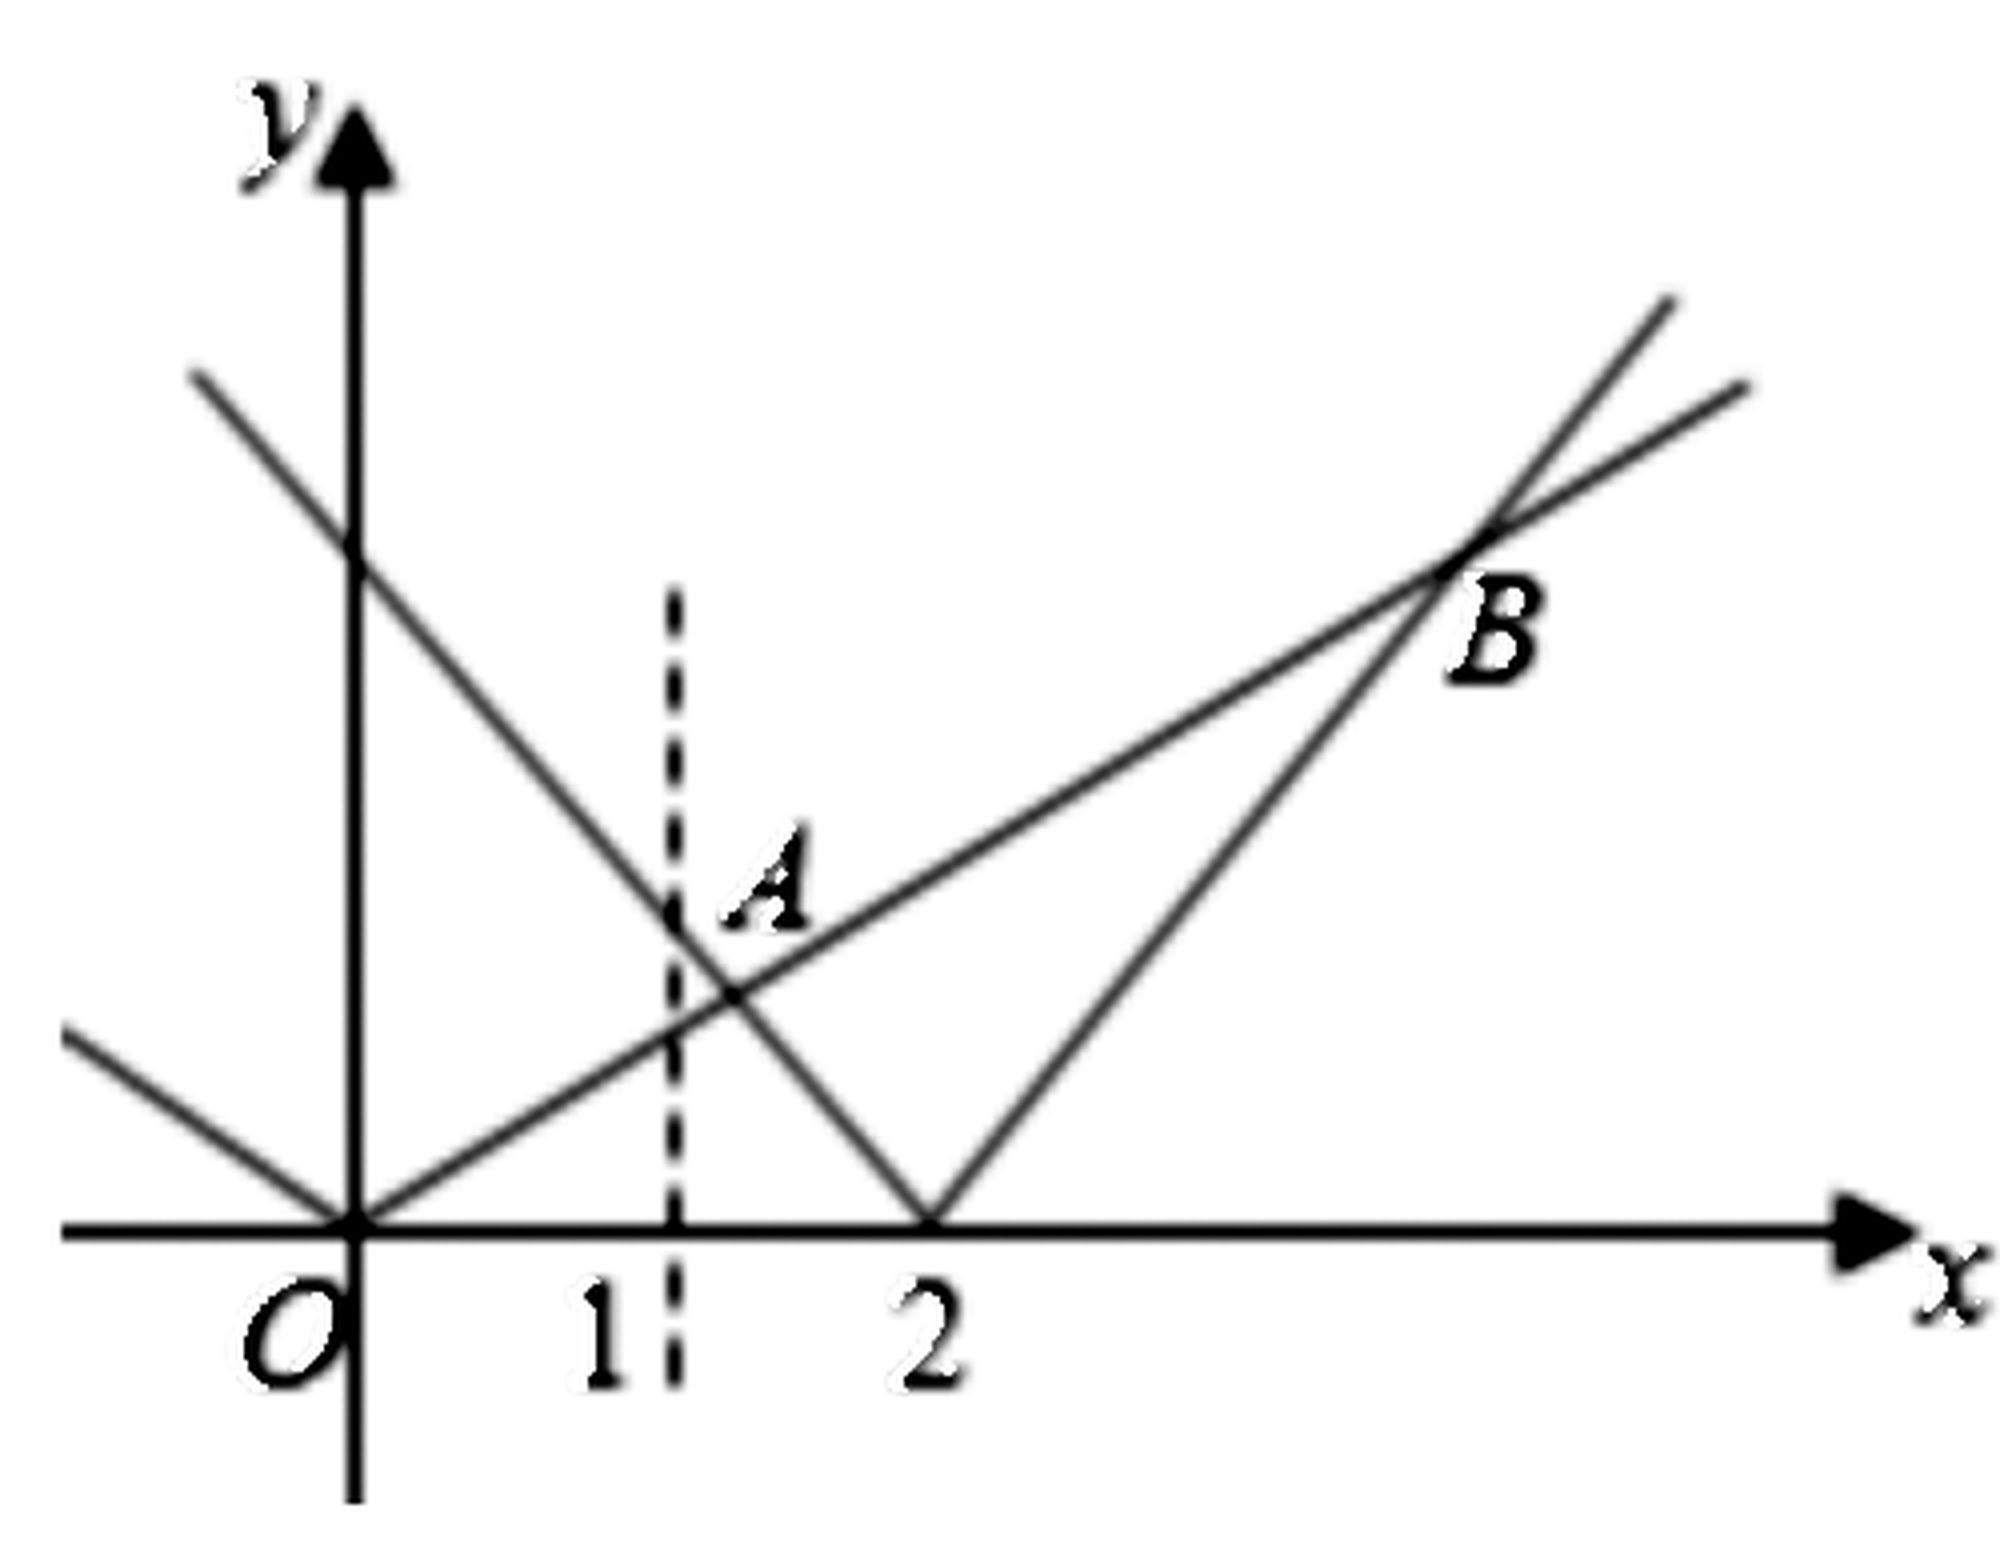
\includegraphics[width=0.40\textwidth]{figures/gao152_q15.png}
\end{center}
\step{由 $0<k<1$，得 $x_A>1$，}
\step{所以关于 $x$ 的不等式 $k\lvert x\rvert-\lvert x-2\rvert>0$ 恰好有 4 个整数解，是 2，3，4，5，}
\step{由 $\begin{cases}y=kx\\y=x-2\end{cases}\Rightarrow x_B=\dfrac2{1-k}\in(5,6]$，故 $\dfrac35<k\leqslant\dfrac23$；故选 $B$.}
\solend
\fi

% === Q16 === 咖啡优惠题；解析 12 行（跨 04 页上下半）；故选 C
\item 上海是全球咖啡店最多的城市. 若某品牌的某种在售咖啡产品价格为 30 元/杯，其原材料成本为 7 元/杯，营销成本为 5 元/杯，且该品牌门店提供如下 4 种优惠方式：(1) 首杯免单，每人限用一次；(2) 3.8 折优惠券，每人限用一次；(3) 买 2 杯送 2 杯，每人限用两次；(4) 买 5 杯送 5 杯，不限使用人数和使用次数. 每位消费者都可以在以上 4 种优惠方式中选择不多于 2 种使用. 现在某个公司有 5 位后勤工作人员去该品牌门店帮每位技术人员购买 1 杯咖啡，购买杯数与技术人员人数须保持一致；请问，这个公司的技术人员不少于\mbox{（\quad）}人时，无论 5 位后勤人员采用什么样的优惠方式购买咖啡，这笔订单该品牌门店都能保证盈利.

\keepwithprev
A. 20\qquad\qquad B. 25\qquad\qquad C. 30\qquad\qquad D. 35

\ifanswer
\solbegin
\step{按各优惠不叠加于同一杯理解，3.8 折券仅用于一杯，}
\step{买赠中的购买杯按原价付款.}
\step{设共购 $n$ 杯，免单、券购、原价购买的杯数分别为 $a,b,c$，其中 $0\leqslant a,b\leqslant5$，}
\step{其余为买赠咖啡，每杯成本为 12 元，}
\step{利润为 $P=15(n-a-b-c)+11.4b+30c-12n=3n-15a-3.6b+15c$，}
\step{若 $a,b$ 不同时为 5，则 $15a+3.6b\leqslant75+14.4=89.4$，}
\step{当 $n\geqslant30$ 时，$P\geqslant90-89.4=0.6>0$.}
\step{若 $a=b=5$，则每人均已使用免单和优惠券两种方式，其余均须原价购买，}
\step{$P=57+30(n-10)-12n=18n-243\geqslant297>0$.}
\step{当 $n=29$ 时，4 人各用方式 (1)(2) 购得 2 杯，}
\step{另 1 人用方式 (1) 及两次方式 (4) 购得 21 杯，}
\step{此时 $P=4\times11.4+2\times150-29\times12=-2.4<0$，因此最小人数为 30，故选 $C$.}% $2\times150$ 为两次方式（4）各买 5 杯的付款，照录（见 ⑤ 3）
\solend
\fi

\end{enumerate}

\bigsec{三、解答题}

\begin{enumerate}
\setcounter{enumi}{16}

% === Q17 === 解集含 \R／\varnothing；解析 4 行
\item 若 $a$、$b\in\R$，求关于 $x$ 的不等式 $ax\geqslant b$ 的解集.

\ifanswer
\solbegin
\step{当 $a>0$ 时，原不等式的解集为 $\left\{x\mid x\geqslant\dfrac ba\right\}$；}
\step{当 $a<0$ 时，原不等式的解集为 $\left\{x\mid x\leqslant\dfrac ba\right\}$；}
\step{当 $a=0$，$b\leqslant0$ 时，原不等式的解集为 $\R$；}
\step{当 $a=0$，$b>0$ 时，原不等式的解集为 $\varnothing$.}
\solend
\fi

% === Q18 === 子集 ⊆ 两处照录；cases 块；解析 9 行（跨 05 页上下半）
\item 已知 $\alpha:x<3m-1$ 或 $x>-m$，$\beta:x<2$ 或 $x\geqslant4$.

(1) 若 $\alpha$ 是 $\beta$ 的充分条件，求实数 $m$ 的取值范围；

(2) 若 $\alpha$ 是 $\beta$ 的必要条件，求实数 $m$ 的取值范围.

\ifanswer
\solbegin
\step{(1) 设 $A=\{x\mid x<3m-1\text{ 或 }x>-m\}$，$B=\{x\mid x<2\text{ 或 }x\geqslant4\}$，}
\step{因为 $\alpha$ 是 $\beta$ 的充分条件，所以 $A\subseteq B$，}
\step{当 $3m-1>-m$ 时，即 $m>\dfrac14$，此时 $A=\R$，不满足题意；}
\step{当 $3m-1\leqslant-m$ 时，即 $m\leqslant\dfrac14$，有 $\begin{cases}3m-1\leqslant2\\-m\geqslant4\end{cases}$，解得 $m\leqslant-4$；}
\step{综上，$m$ 的取值范围为 $(-\infty,-4]$.}
\step{(2) 因为 $\alpha$ 是 $\beta$ 的必要条件，所以 $B\subseteq A$，}
\step{当 $3m-1>-m$ 时，即 $m>\dfrac14$，此时 $A=\R$，$B\subseteq A$ 成立；}
\step{当 $3m-1\leqslant-m$ 时，即 $m\leqslant\dfrac14$，有 $\begin{cases}3m-1\geqslant2\\-m<4\end{cases}$，无解.}
\step{综上，$m$ 的取值范围为 $\left[\dfrac14,+\infty\right)$.}
\solend
\fi

% === Q19 === \varnothing 空集照录；解析 9 行
\item 设关于 $x$ 的不等式 $x^2+4x+k-1\geqslant0$ 的解集为 $A$.

(1) 若 $A=\R$，求实数 $k$ 的取值范围；

(2) 求证：不存在实数 $k$，使得 $A=\varnothing$.

\ifanswer
\solbegin
\step{(1) 配方得 $x^2+4x+k-1=(x+2)^2+k-5$，}
\step{若 $A=\R$，取 $x=-2$，得 $k-5\geqslant0$，即 $k\geqslant5$.}
\step{当 $k\geqslant5$ 时，对任意 $x\in\R$，都有 $(x+2)^2+k-5\geqslant0$，因此 $A=\R$.}
\step{所以 $k$ 的取值范围为 $[5,+\infty)$.}
\step{(2) 当 $k\geqslant5$ 时，由 (1) 得 $A=\R\ne\varnothing$.}
\step{当 $k<5$ 时，取 $x_0=-2+\sqrt{5-k}$，}
\step{则 $x_0^2+4x_0+k-1=(x_0+2)^2+k-5=(5-k)+k-5=0$，}
\step{所以 $x_0\in A$，即 $A\ne\varnothing$.}
\step{因此，不存在实数 $k$，使得 $A=\varnothing$.}
\solend
\fi

% === Q20 === |A\cap B|=1 印等号；等腰偏高粗 \Delta 照录；解析 12 行（跨 06→07 页）
\item 设 $m\in\R$. 集合 $A=\left\{x\mid\dfrac{x^2+x}{x+1}\geqslant\dfrac{2x+m}{x},x\in\R\right\}$，
$B=\left\{x\mid\dfrac{x^2+x}{x+1}\leqslant\dfrac{2x+m}{x},x\in\R\right\}$.

(1) 若 $m=8$，记集合 $M=A\cap(0,+\infty)$，求集合 $M$；

(2) 用 $\lvert T\rvert$ 代表集合 $T$ 的元素个数. 若 $\lvert A\cap B\rvert=1$，记 $m$ 的取值集合为 $C$，试比较 $\lvert C\rvert$ 与 2 的大小，并证明你的结论.

\ifanswer
\solbegin
\step{(1) 当 $m=8$，$x>0$ 时，$\dfrac{x^2+x}{x+1}\geqslant\dfrac{2x+8}{x}\Leftrightarrow x^2-2x-8\geqslant0$}
\step{$\Leftrightarrow(x-4)(x+2)\geqslant0\Leftrightarrow x\geqslant4$，所以 $M=[4,+\infty)$.}
\step{(2) 原分式有意义须 $x\ne-1,0$，因此 $x\in A\cap B\Leftrightarrow\begin{cases}x^2-2x-m=0\\x\ne-1,0\end{cases}$，}
\step{方程的判别式为 $\Delta=4(1+m)$.}
\step{当 $m<-1$ 时，方程无实根，$\lvert A\cap B\rvert=0$；}
\step{当 $m=-1$ 时，方程只有一个实根 1，$A\cap B=\{1\}$.}
\step{当 $m>-1$ 时，方程有两个不同实根.}
\step{其中，0 为根当且仅当 $m=0$，$-1$ 为根当且仅当 $m=3$.}
\step{$m=0$ 时，方程的根为 $0,2$，$A\cap B=\{2\}$；}
\step{$m=3$ 时，方程的根为 $-1,3$，$A\cap B=\{3\}$.}
\step{$m>-1$ 且 $m\ne0,3$ 时，两个实根均满足原分式的定义条件，$\lvert A\cap B\rvert=2$.}
\step{因此 $C=\{-1,0,3\}$，$\lvert C\rvert=3>2$.}
\solend
\fi

% === Q21 === "性质 p"新定义、\Q 归一、M\subseteq\R 照录；解析 19 行（跨 07→08 页）
\item 设集合 $M\subseteq\R$. 若 $M$ 中元素个数大于等于 2，且 $M$ 的任意不同元素 $a$、$b$ 均满足 $a^3-\dfrac14b\in M$，则称集合 $M$ 具有“性质 $p$”.

(1) 试判断集合 $\Q$、集合 $\left\{-\dfrac{\sqrt3}{2},0,\dfrac{\sqrt3}{2}\right\}$ 是否具有“性质 $p$”，并说明理由；

(2) 设 $m$ 为大于等于 2 的正整数. 若集合 $A=\{x_1,x_2,\cdots,x_m\}$，且具有“性质 $p$”，求证：$m=2$，并求集合 $A$ 中所有元素的乘积.

\ifanswer
\solbegin
\step{(1) $\Q$ 中至少有两个元素，且任意不同的 $a,b\in\Q$ 均满足 $a^3-\dfrac14b\in\Q$，}
\step{故 $\Q$ 具有“性质 $p$”.}
\step{对于另一集合，取 $a=0$，$b=\dfrac{\sqrt3}{2}$，则 $a^3-\dfrac14b=-\dfrac{\sqrt3}{8}$ 不属于该集合，}
\step{故其不具有“性质 $p$”.}
\step{(2) 将 $A$ 中元素按 $x_1<x_2<\cdots<x_m$ 排列.}
\step{若 $m\geqslant3$，由性质 $p$ 及幂函数 $y=x^3$ 的单调性，}
\step{有 $x_1^3-\dfrac14x_m<\cdots<x_1^3-\dfrac14x_2<x_m^3-\dfrac14x_2<x_m^3-\dfrac14x_1$，}
\step{上述 $m+1$ 个互不相同的数均属于 $A$，与 $A$ 只有 $m$ 个元素矛盾，}
\step{因此 $m=2$.}
\step{设 $A=\{a,b\}$，$a<b$.}
\step{因为 $a^3-\dfrac14b<b^3-\dfrac14a$，且两者均属于 $A$，}
\step{所以 $a^3-\dfrac14b=a$，$b^3-\dfrac14a=b$，}
\step{两式相减并除以 $a-b\ne0$，}
\step{以及两式相加，分别得 $a^2+ab+b^2=\dfrac34$，$(a+b)(a^2-ab+b^2)=\dfrac54(a+b)$，}
\step{代入 $a^2-ab+b^2=\dfrac34-2ab$，得 $(a+b)(4ab+1)=0$，}
\step{若 $a+b=0$，则 $-ab=a^2+ab+b^2=\dfrac34$，即 $ab=-\dfrac34$；}
\step{若 $a+b\ne0$，则 $ab=-\dfrac14$.}
\step{分别取 $A=\left\{-\dfrac{\sqrt3}{2},\dfrac{\sqrt3}{2}\right\}$，$A=\left\{\dfrac{1-\sqrt3}{2\sqrt2},\dfrac{1+\sqrt3}{2\sqrt2}\right\}$，}
\step{代入均有 $a^3-\dfrac14b=a$、$b^3-\dfrac14a=b$，故两种乘积均可取得.}
\solend
\fi

\end{enumerate}

\end{document}
"
%
% ① 原始材料：微信公众号"魔都数学加油站"文章，连载"27学年高一152"，原文标题
% "27学年高一152——2026-2027年上海市位育中学高一上期中"；
% 原文链接：https://mp.weixin.qq.com/s/v4_G6oTX2BuPz9L-KtLRfw 。
% 正文为 8 张 PNG 页（01/03/05/06/07/08 为 2560×3620，02/04 为 4762×6735，
% 同一篇各页分辨率混排，逐页按各自分辨率裁图核对，别按预览比例换算裁框）。
% 体例：讲评版——填空 3—12（10 题）、选择 13—16（4 题）、解答 17—21（5 题），
% 共 19 题，自第 3 题起编；题目、答案、解析均据原图转录；卷面粉红色水印
% "魔都数学加油站"及公众号页脚未录入。
% 全卷插图清单（逐页通读 8 页确认）：1 幅——第 15 题解析配图（两条折线
% $y=k\lvert x\rvert$ 与 $y=\lvert x-2\rvert$ 及坐标图，03 页右下，含 O、1、2、
% A、B 与虚线 $x=1$），解析写"的图象如下"，仅答案版出，裁
% figures/gao152_q15.png（去粉水印、去色、4× LANCZOS 放大）。
%
% 卷首标题：原卷印作"2026-2027 年位育中学高一上期中"，年份区间按全稿惯例排 en dash；
% 原卷卷面未印副标题，本稿按同期中卷知识模块口径补出"集合与常用逻辑用语、不等式、函数"。
%
% ② 与原卷的排版差异：
%   ① 原文从第 3 题起，本稿保留原题号；共 19 题三节，解答题 5 题到 21；
%   ② 混合体例：第 3、5 题只印【答案】、无【解析】，按 高一140 第 5 题／
%      高一145 第 3 题成例另提 \ans{}、不补造解析；第 13、14 题把答案"D"
%      直接印在题干括号内、题下无【解析】，按 高一84／148／149 成例括号留空、
%      另提 \ans{$D$}；其余 15 题印【解析】、用 \solbegin…\solend；
%      第 15、16 题答案在解析末句"故选 B／C"、括号留空、不另提 \ans{}；
%      答案版【答案】/【解析】标记数 = 19 = 全卷题数（4 个 \ans ＋ 15 个 \solbegin）；
%   ③ 原卷卷面未印副标题，本稿按知识模块口径补出；
%   ④ 原卷填空横线按全稿惯例排 \blankline[4.4em]；选择题括号排 \mbox{（\quad）}、
%      四道选择题的选项段前按惯例各加 \keepwithprev；解答题不留作答区、不加
%      \anspace（原卷为讲评版，109—113 起全稿不用 \anspace）；
%   ⑤ 数集黑板粗体：Q7"全集为 R"、Q9"$\lVert PQ\rVert$ 定义"无数集、
%      Q12"$t\in Z$"、Q13"$k\in Z$ 与 $=\R$"、Q17"$a,b\in R$"、Q19"$A=\R$"、
%      Q20"$m\in\R$"、Q21"$M\subseteq\R$ 与集合 $\Q$"原卷印正体粗体或黑板体
%      R/Q/Z，按全稿惯例归一 \R／\Q／\Z；绝对值排 \lvert…\rvert
%      （Q4、Q9、Q11、Q15），集合描述竖线排 \mid（Q7、Q13、Q20、Q21），
%      距离双竖线排 \lVert…\rVert（Q9 与题干、解析的 ||PQ||／||AB||）；
%      不等号按全稿惯例排 \leqslant／\geqslant；补集照原卷上划线排 \overline{A}
%      （Q7 题干＋解析）；空集 \varnothing（Q17、Q19）；
%      子集 Q18 两处、Q21 题干一处均印带下划线 ⊆、照录 \subseteq（见 ④），
%      本卷无单线 \subset 用例；
%   ⑥ 判别式 Δ/△ 两形混用逐处照录、不得统一：Q11 解析"判别式 △=k²−8k>0"
%      印扁等边细线三角、照录 \triangle，Q20 (2) 解析"判别式为 Δ=4(1+m)"
%      印等腰偏高粗三角、照录 \Delta（/tmp/gao152/z/zoom/q11_delta.png、
%      q20_delta.png 放大并与 151 卷同型并排比较）；
%   ⑦ 中文弯引号照录：Q11"长度"、Q21"性质 p"（题干、两问与解析多处）、
%      Q6 从">"、"<"、"≥"、"≤"中选符号、Q16"（1）…（4）"半角括号；
%      注释里一律 ASCII 引号；数学式内 CJK 用 \text{}（Q13 的"或／且"、
%      Q18 集合描述的"或"）；
%   ⑧ "图像／图象"：全卷仅 Q15 解析一处"的图象如下"，印"图象"（象，无亻）、
%      照录；其余各题无"图像"字样。子题标号 (1)(2)(3)(4) 半角括号照录；
%   ⑨ 半角逗号在数学组之间是全稿惯例、非笔误，逐处照录（Q6、Q10、Q16、
%      Q20、Q21 的 $a,b,c$ 之类）；行末西文句点 ASCII `.`；
%      行中全角逗号／顿号照录（Q11"（a,b）"、Q16"7 元/杯"、Q21"$\Q$、集合"）；
%   ⑩ 复杂式照录别简化：Q4 四组 cases 块（整体各占一个印刷行）、Q8
%      $\frac{x_0}{e^{x_0}}=\frac13$、Q10 $4a^2+b^2=4$、Q12 $b=\frac2a$、
%      Q16 利润式 $P=15(n-a-b-c)+11.4b+30c-12n$、Q18 cases 块、
%      Q20 分式 $\frac{x^2+x}{x+1}$、Q21 $a^3-\frac14b$ 与两组取值集合；
%      \left…\right 不得拆到不同 $…$ 组（Q4 cases 前的 \left\{ 一律改
%      \begin{cases}…\end{cases}、Q17 $\left\{x\mid x\ge\frac ba\right\}$、
%      Q20 $\left\{x\mid\cdots\right\}$、Q21 $\left\{-\frac{\sqrt3}2,\ldots\right\}$）；
%   ⑪ 一条 \step = 原卷解析的一个印刷行，cases 块整体算一个印刷行；别并折行、
%      别拆行。Q12 七行、Q16 十二行、Q18 九行、Q19 九行、Q20 十二行、
%      Q21 十九行均按印刷行逐条断，不丢行；
%   ⑫ 配图：Q15 解析配图（仅答案版出）放 \ifanswer 内 \solbegin…\solend 的
%      \step 之间（高一73 第 16 题／高一150 Q12 成例）；题干无配图，故无
%      \needvspace；
%   ⑬ 原卷解析内无红色"法一／法二"之类小标题，故本卷无 \stepm；红色水印
%      "魔都数学加油站"不录入；
%   ⑭ 跨页续印按题合并：见 ⑥；
%
% ③ 行数复核：一条 \step = 原卷解析的一个印刷行，cases 块作一个印刷行计。
%   逐题数（主会话逐页核对定稿）：Q3：0（只印【答案】、提 \ans{}）；Q4：2；
%   Q5：0（只印【答案】、提 \ans{}）；Q6：1；Q7：1；Q8：1；Q9：1；
%   Q10：4；Q11：5；Q12：7；Q13：0（答案印括号内、提 \ans{}）；
%   Q14：0（答案印括号内、提 \ans{}）；Q15：4；Q16：12；Q17：4；
%   Q18：9；Q19：9；Q20：12；Q21：19。
%   合计 91 条 \step（本卷无 \stepm），与原卷逐题印刷行相等。全卷 15 题设
%   \solbegin…\solend ＋ Q3／Q5／Q13／Q14 四处 \ans{}，答案版
%   【答案】/【解析】标记数 = 19 = 全卷题数。
%
% ④ 判别式／子集符号结论（逐处放大原图照录、不得统一，主会话像素级复核）：
%   判别式：Q11 解析"方程 $x^2-kx+2k=0$ 的判别式 $\triangle=k^2-8k>0$"
%      印扁等边细线三角、照录 \triangle；Q20 (2) 解析"方程的判别式为
%      $\Delta=4(1+m)$"印等腰偏高粗三角、照录 \Delta
%      （/tmp/gao152/z/zoom/q11_delta.png、q20_delta.png；与 高一142／151
%      的"Δ/△ 混用逐处照录"口径一致）。本卷无几何三角形符号。
%   子集：Q18 解析 (1)"$A\subseteq B$"、(2)"$B\subseteq A$"与 Q21 题干
%      "$M\subseteq\R$"共 3 处均印带下划线 ⊆、照录 \subseteq
%      （/tmp/gao152/z/zoom/q18_subset.png、q21_subset.png 放大确认）；
%      本卷无单线 ⊂ 用例。补集上划线 \overline{A}（Q7）、空集 \varnothing
%      （Q17 解析末行、Q19 题干 (2) 与解析）、数集 \R／\Q／\Z 归一见 ② ⑤。
%
% ⑤ 存疑照录（放大原图确认，照录未改、正文对应处另有 % 注）：
%   1. Q11 题干"已知关于 $x$ 的不等式 $x^2-kx+2k<0$ 有实数解，且解集区间
%      长度不超过 3 个单位"，解析据 $\lvert x_1-x_2\rvert\leqslant3$ 推；
%      判别式用扁三角 \triangle（见 ④），照录未改。
%   2. Q12 解析"$t=-1$ 时取 $b=\frac2a\in[-2,-1]$，$c=-1$，则 $ab+c=2-1=1$"
%      ——$b$ 径写 $\frac2a$（无负号），放大 03 页确认，照录未改。
%   3. Q16 解析"$P=4\times11.4+2\times150-29\times12=-2.4<0$"中的
%      $2\times150$ 为两次方式（4）各买 5 杯的付款，照录未改。
%   4. Q20 (2) 题干"若 $\lvert A\cap B\rvert=1$"印等号（非 $\leqslant1$），
%      放大 06 页 /tmp/gao152/z/zoom/q20_eq1.png 确认，照录未改。
%   5. Q21 题干"性质 p"用弯引号且 $p$ 为斜体小写，逐处照录未统一；
%      解析 (2) 末两组 $A$ 的取值集合照录未简化。
%   6. "图像／图象"仅 Q15 一处"图象"、Δ/△ 两形并用（Q11 \triangle、
%      Q20 \Delta）均逐处照录、未统一（见 ② ⑥ ⑧ 与 ④）。
%   全卷除此 6 类外未发现其它笔误／自相矛盾处；19 题中 15 题印【解析】、
%   Q3／Q5 只印【答案】、Q13／Q14 答案印题干括号内（见 ② ②）。
%
% ⑥ 跨页续印按题合并说明（逐页核实定稿）：Q3—Q5 题干＋【答案】／【解析】
%   在 01 页上半，Q6—Q8 题干＋解析在 01 页下半；Q9、Q10 题干＋解析、
%   Q11 题干＋解析、Q12 题干＋解析首行在 02 页；Q12 解析余 6 行续 03 页
%   上半，"二、选择题"标题与 Q13 题干＋选项在 03 页下半；Q13 选项 C／D、
%   Q14 题干＋四选项＋（无解析）、Q15 题干＋四选项＋解析前 3 行＋配图在
%   03 页下半，Q15 解析末行（由 cases 求 $x_B$）续 04 页顶；Q16 题干＋四选项
%   ＋解析前 5 行在 04 页上半，解析余 7 行在 04 页下半；"三、解答题"标题与
%   Q17 题干＋解析首行在 04 页末，Q17 解析余 3 行、Q18 题干＋两问＋解析首
%   4 行在 05 页上半，Q18 解析余 5 行在 05 页下半；Q19 题干＋两问＋解析
%   (1) 4 行在 05—06 页（(2) 题干续 06 页顶），解析 (2) 5 行在 06 页上半；
%   Q20 题干＋两问＋解析 (1) 2 行＋(2) 首行在 06 页下半；Q20 (2) 解析余
%   9 行、Q21 题干＋两问＋解析 (1) 4 行在 07 页；Q21 (2) 解析 19 行中前
%   6 行在 07—08 页上半、末 13 行续 08 页下半，末行"故两种乘积均可取得"
%   为全卷收尾（08 页下半仅水印、无其它正文）。
%   本稿按题连排，不丢行、不并折行；全卷末题为第 21 题，无附加题节。
%
\documentclass[a4paper,11pt]{article}
\usepackage{common}

\begin{document}

\examtitlest[3]{2026--2027 年位育中学高一上期中}{集合与常用逻辑用语、不等式、函数}

\bigsec{一、填空题}

\begin{enumerate}
\setcounter{enumi}{2}

% === Q3 === 原卷只印【答案】、无【解析】，另提 \ans{}，不补造解析
\item 设 $x>0$. 若 $\ln x=-1$，则 $x=$\blankline[4.4em].

\ifanswer
\ans{$\dfrac1{\mathrm{e}}$}
\fi

% === Q4 === 四组 cases 块同一印刷行；解析 2 行
\item 不等式 $\lvert 1-2x\rvert>x$ 的解集为\blankline[4.4em].

\ifanswer
\solbegin
\step{不等式 $\lvert 1-2x\rvert>x$ 即为 $\begin{cases}1-2x\geqslant0\\1-2x>x\end{cases}$ 或 $\begin{cases}1-2x<0\\2x-1>x\end{cases}$，即 $\begin{cases}x\leqslant\frac12\\x<\frac13\end{cases}$ 或 $\begin{cases}x>\frac12\\x>1\end{cases}$，}
\step{则有 $x<\dfrac13$ 或 $x>1$，则解集为 $\left(-\infty,\dfrac13\right)\cup(1,+\infty)$.}
\solend
\fi

% === Q5 === 原卷只印【答案】、无【解析】；\frac1x\ge1 印单线 ≥，按全稿惯例 \geqslant
\item 不等式 $\dfrac1x\geqslant1$ 的解集为\blankline[4.4em].

\ifanswer
\ans{$(0,1]$}
\fi

% === Q6 === 从四个符号中选一个，中文弯引号照录；解析 1 行
\item 设 $a$、$b>0$，则 $a^2+b^2$\blankline[4.4em]$2(2a-b)-5$（从“$>$”、“$<$”、“$\geqslant$”、“$\leqslant$”中选择一个符号填写）.

\ifanswer
\solbegin
\step{$a^2+b^2-[2(2a-b)-5]=(a-2)^2+(b+1)^2>0$，故 $a^2+b^2>2(2a-b)-5$.}
\solend
\fi

% === Q7 === 补集上划线 \overline{A}；集合描述竖线 \mid；解析 1 行
\item 已知全集为 $\R$，集合 $A=\{x\mid y=\sqrt{x-2}\}$，集合 $B=\{y\mid y=\sqrt{x-2}\}$，则 $\overline{A}\cap B=$\blankline[4.4em].

\ifanswer
\solbegin
\step{$A=[2,+\infty)$，$B=[0,+\infty)$，所以 $\overline{A}\cap B=[0,2)$.}
\solend
\fi

% === Q8 === \frac{x_0}{e^{x_0}}=\frac13 照录；解析 1 行
\item 设正数 $x_0$ 满足等式 $\dfrac{x_0}{e^{x_0}}=\dfrac13$，则 $x_0-\ln x_0=$\blankline[4.4em].

\ifanswer
\solbegin
\step{等式两边取自然对数，得 $\ln x_0-x_0=-\ln3$，即 $x_0-\ln x_0=\ln3$.}
\solend
\fi

% === Q9 === 距离双竖线 \lVert…\rVert；解析 1 行
\item 在平面直角坐标系 $xOy$ 中，设点 $P(x_1,y_1)$，$Q(x_2,y_2)$，定义：$\lVert PQ\rVert=\lvert x_1-x_2\rvert+\lvert y_1-y_2\rvert$. 若点 $A(1,0)$，点 $B$ 为直线 $y=x+2$ 上的动点，则 $\lVert AB\rVert$ 的最小值为\blankline[4.4em].

\ifanswer
\solbegin
\step{$\lVert AB\rVert=\lvert x-1\rvert+\lvert y\rvert=\lvert x-1\rvert+\lvert x+2\rvert\geqslant3$，最小值为 3.}
\solend
\fi

% === Q10 === 解析 4 行
\item 已知 $a$、$b$ 均为正数，且 $a^2+\dfrac14b^2=1$，则 $a\sqrt{1+b^2}$ 的最大值为\blankline[4.4em].

\ifanswer
\solbegin
\step{因为 $a$、$b$ 均为正数，且 $a^2+\dfrac14b^2=1$，所以 $4a^2+b^2=4$，}
\step{所以 $a\sqrt{1+b^2}=\dfrac12\cdot2a\cdot\sqrt{1+b^2}\leqslant\dfrac12\cdot\dfrac{4a^2+1+b^2}{2}=\dfrac54$，}
\step{当且仅当 $4a^2=b^2+1$ 即 $a=\dfrac{\sqrt{10}}4$，$b=\dfrac{\sqrt6}2$ 时取等号，}
\step{故 $a\sqrt{1+b^2}$ 的最大值为 $\dfrac54$.}
\solend
\fi

% === Q11 === 扁等边细线判别式 \triangle 照录（见 ④）；"长度"弯引号；解析 5 行
\item 一般地，把 $b-a$ 称为区间 $(a,b)$ 的“长度”. 已知关于 $x$ 的不等式 $x^2-kx+2k<0$ 有实数解，且解集区间长度不超过 3 个单位，则实数 $k$ 的取值范围是\blankline[4.4em].

\ifanswer
\solbegin
\step{因为不等式 $x^2-kx+2k<0$ 有解，}
\step{所以方程 $x^2-kx+2k=0$ 的判别式 $\triangle=k^2-8k>0$，解得 $k>8$ 或 $k<0$，}
\step{由 $x_1+x_2=k$，$x_1x_2=2k$，得 $(x_1-x_2)^2=(x_1+x_2)^2-4x_1x_2=k^2-8k$，}
\step{由 $\lvert x_1-x_2\rvert\leqslant3$，得 $(x_1-x_2)^2\leqslant9$，即 $k^2-8k\leqslant9$，解得 $-1\leqslant k\leqslant9$，}
\step{所以 $-1\leqslant k<0$ 或 $8<k\leqslant9$，即实数 $k$ 的取值范围是 $[-1,0)\cup(8,9]$.}
\solend
\fi

% === Q12 === $b=\frac2a$ 无负号、$c=-1$ 照录（见 ⑤ 2）；解析 7 行（跨 02→03 页）
\item 设 $t\in\Z$，且对任意 $a\in[-2,t]$，总存在 $b,c\in[-2,t]$，使得 $ab+c=1$，则 $t$ 的所有取值为\blankline[4.4em].

\ifanswer
\solbegin
\step{$[-2,t]$ 是区间，要求 $t>-2$，故 $t\geqslant-1$.}
\step{当 $t\geqslant1$ 时，对任意 $a\in[-2,t]$，}
\step{取 $b=0$，$c=1$，两者都属于 $[-2,t]$，且 $ab+c=1$.}
\step{当 $t=0$ 时，取 $a=0$，则 $c=1\notin[-2,0]$，不成立.}
\step{当 $t=-1$ 时，对任意 $a\in[-2,-1]$，取 $b=\dfrac2a\in[-2,-1]$，$c=-1$，}% 原卷径写 $b=\frac2a$（无负号），放大 03 页确认，照录未改（见 ⑤ 2）
\step{则 $ab+c=2-1=1$.}
\step{所以 $t=-1$ 或 $t\geqslant1$（$t\in\Z$）.}
\solend
\fi

\end{enumerate}

\bigsec{二、选择题}

\begin{enumerate}
\setcounter{enumi}{12}

% === Q13 === 答案 D 印在题干括号内、无【解析】，按 高一84／148／149 成例括号留空、另提 \ans{}
\item 下列说法错误的是\mbox{（\quad）}

\keepwithprev
A. 奇数集可以表示为 $\{x\mid x=2k+1,k\in\Z\}$

B. 奇数集可以表示为 $\{x\mid x=2k-1,k\in\Z\}$

C. $\{x\mid x\ne2\text{ 或 }x\ne-2\}=\R$

D. $\{x\mid x\ne2\text{ 且 }x\ne-2\}=\R$

\ifanswer
\ans{$D$}
\fi

% === Q14 === 答案 D 印在题干括号内、无【解析】；选项两行两列
\item 设 $a$、$b$、$c>0$，且 $a\ne1$，则以下代数式中，不恒成立的是\mbox{（\quad）}

\keepwithprev
A. $\log_a 1=0$\qquad\qquad B. $a^{\log_a b}=b$

C. $\log_a b+\log_a c=\log_a(bc)$\qquad\qquad D. $\log_a b=\dfrac1{\log_b a}$

\ifanswer
\ans{$D$}
\fi

% === Q15 === "图象"（象，无亻）照录；解析配图仅答案版出；答案在解析末句故选 B
\item 若关于 $x$ 的不等式 $k\lvert x\rvert>\lvert x-2\rvert$ 恰好有 4 个整数解，则实数 $k$ 的取值范围是\mbox{（\quad）}

\keepwithprev
A. $\left(\dfrac35,\dfrac23\right)$\qquad B. $\left(\dfrac35,\dfrac23\right]$\qquad C. $\left(\dfrac35,1\right)$\qquad D. $\left(\dfrac35,1\right]$

\ifanswer
\solbegin
\step{由题意得 $0<k<1$，函数 $y=k\lvert x\rvert$ 与 $y=\lvert x-2\rvert$ 的图象如下，}
\begin{center}
% 两条折线坐标图取 03 页右下，去粉色水印、去色、4× LANCZOS 放大；仅答案版出
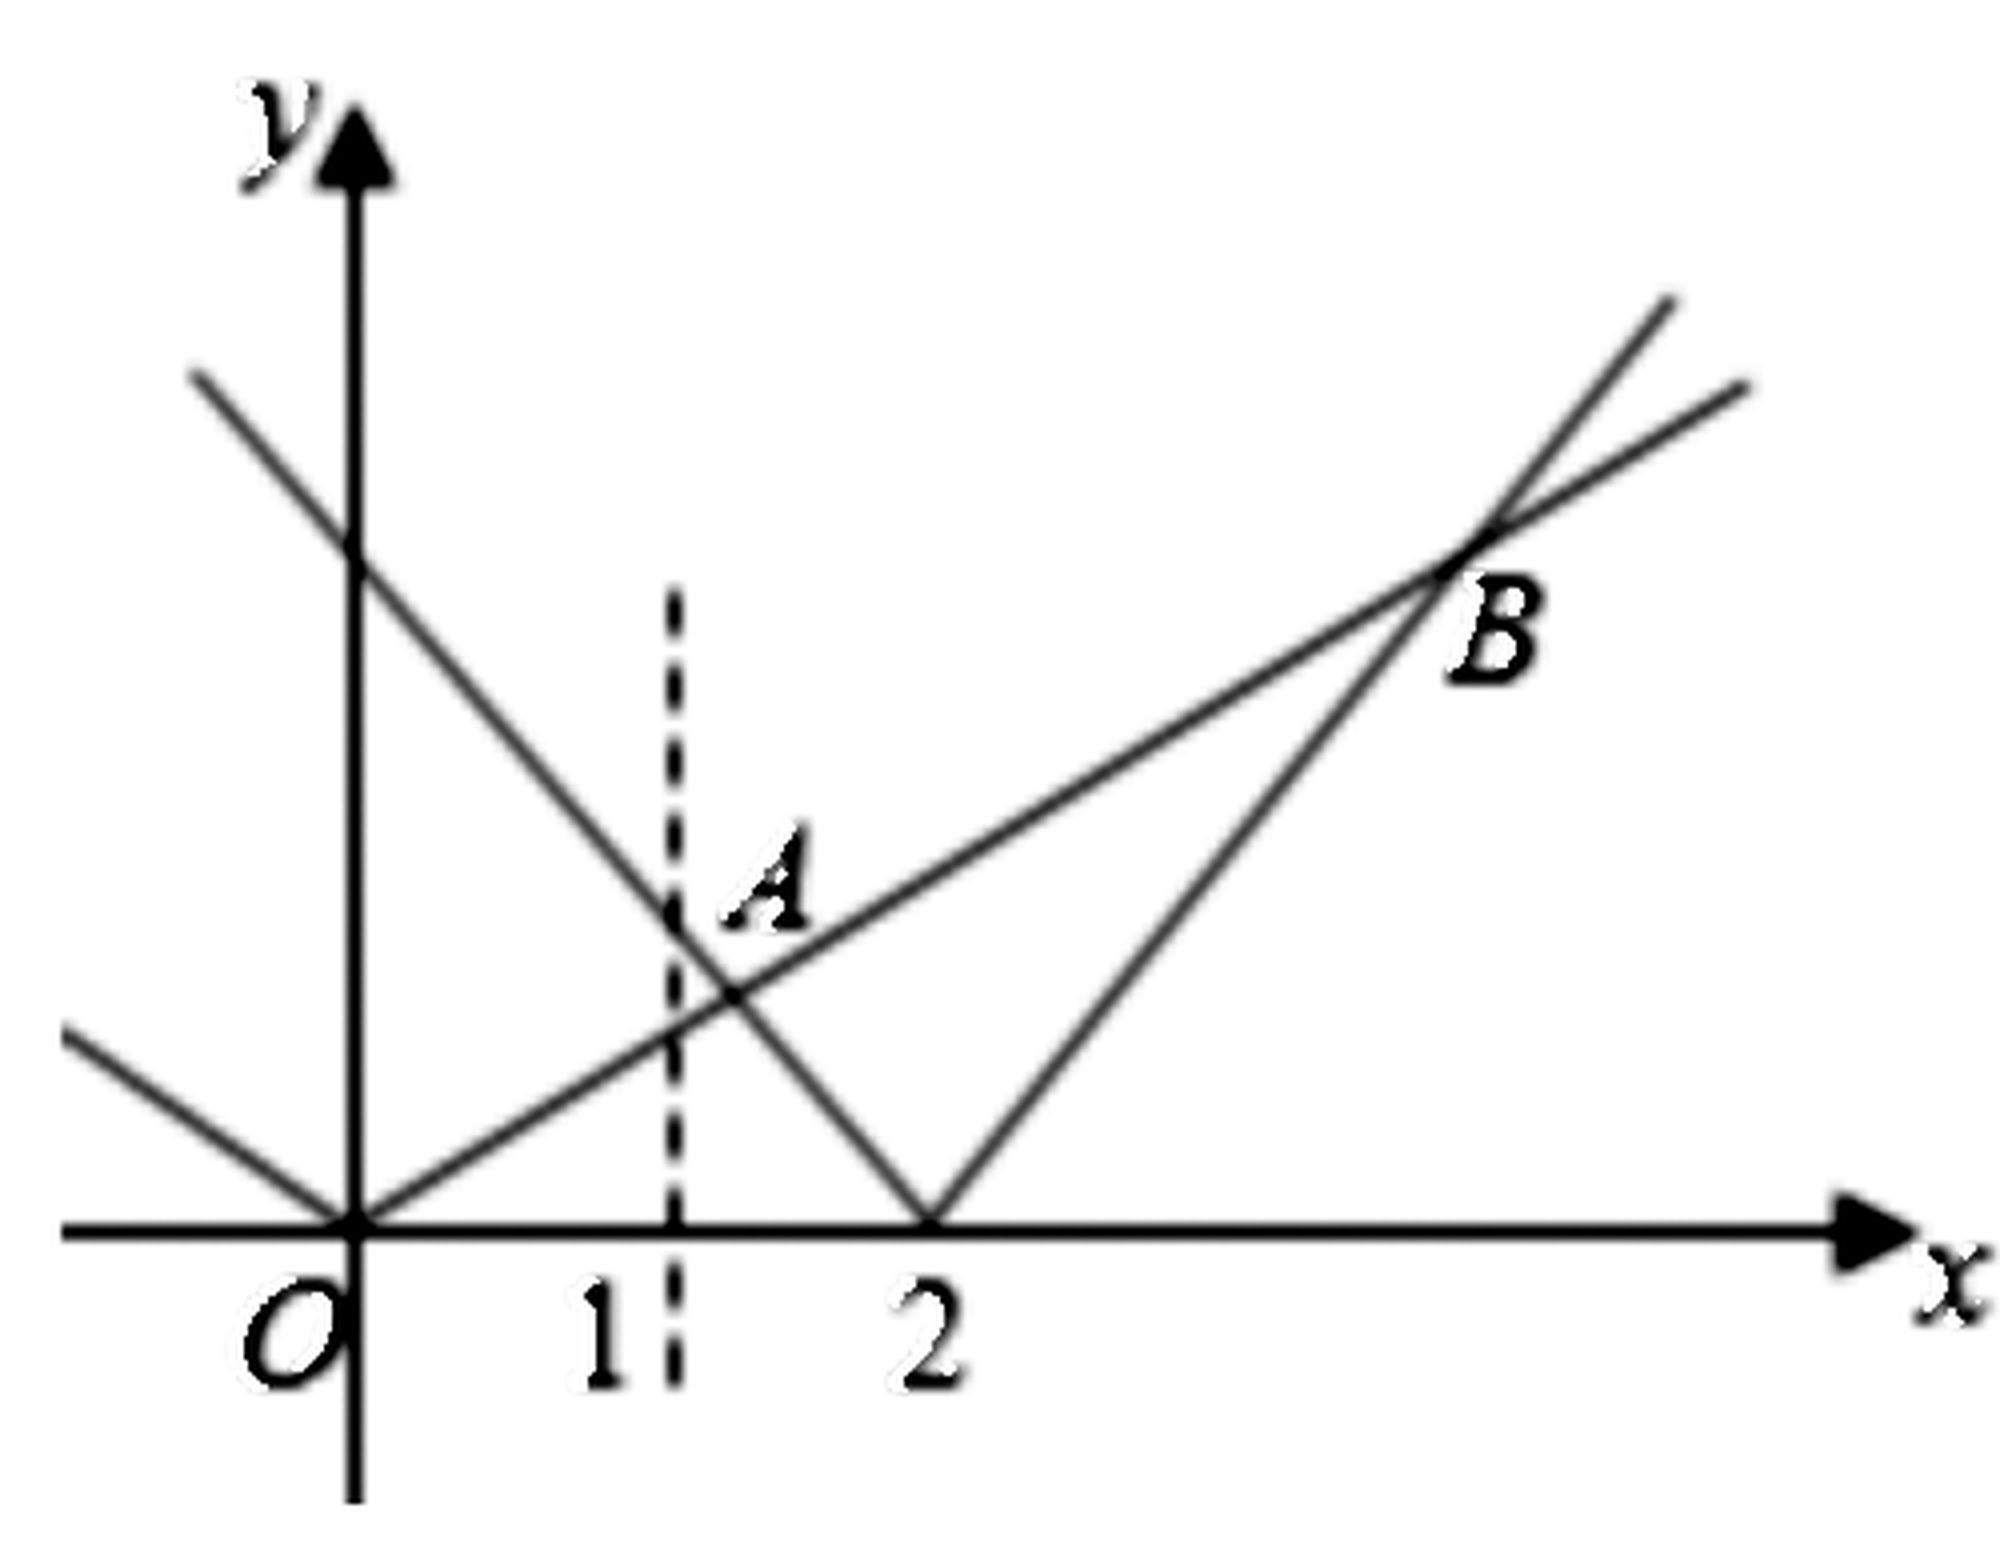
\includegraphics[width=0.40\textwidth]{figures/gao152_q15.png}
\end{center}
\step{由 $0<k<1$，得 $x_A>1$，}
\step{所以关于 $x$ 的不等式 $k\lvert x\rvert-\lvert x-2\rvert>0$ 恰好有 4 个整数解，是 2，3，4，5，}
\step{由 $\begin{cases}y=kx\\y=x-2\end{cases}\Rightarrow x_B=\dfrac2{1-k}\in(5,6]$，故 $\dfrac35<k\leqslant\dfrac23$；故选 $B$.}
\solend
\fi

% === Q16 === 咖啡优惠题；解析 12 行（跨 04 页上下半）；故选 C
\item 上海是全球咖啡店最多的城市. 若某品牌的某种在售咖啡产品价格为 30 元/杯，其原材料成本为 7 元/杯，营销成本为 5 元/杯，且该品牌门店提供如下 4 种优惠方式：(1) 首杯免单，每人限用一次；(2) 3.8 折优惠券，每人限用一次；(3) 买 2 杯送 2 杯，每人限用两次；(4) 买 5 杯送 5 杯，不限使用人数和使用次数. 每位消费者都可以在以上 4 种优惠方式中选择不多于 2 种使用. 现在某个公司有 5 位后勤工作人员去该品牌门店帮每位技术人员购买 1 杯咖啡，购买杯数与技术人员人数须保持一致；请问，这个公司的技术人员不少于\mbox{（\quad）}人时，无论 5 位后勤人员采用什么样的优惠方式购买咖啡，这笔订单该品牌门店都能保证盈利.

\keepwithprev
A. 20\qquad\qquad B. 25\qquad\qquad C. 30\qquad\qquad D. 35

\ifanswer
\solbegin
\step{按各优惠不叠加于同一杯理解，3.8 折券仅用于一杯，}
\step{买赠中的购买杯按原价付款.}
\step{设共购 $n$ 杯，免单、券购、原价购买的杯数分别为 $a,b,c$，其中 $0\leqslant a,b\leqslant5$，}
\step{其余为买赠咖啡，每杯成本为 12 元，}
\step{利润为 $P=15(n-a-b-c)+11.4b+30c-12n=3n-15a-3.6b+15c$，}
\step{若 $a,b$ 不同时为 5，则 $15a+3.6b\leqslant75+14.4=89.4$，}
\step{当 $n\geqslant30$ 时，$P\geqslant90-89.4=0.6>0$.}
\step{若 $a=b=5$，则每人均已使用免单和优惠券两种方式，其余均须原价购买，}
\step{$P=57+30(n-10)-12n=18n-243\geqslant297>0$.}
\step{当 $n=29$ 时，4 人各用方式 (1)(2) 购得 2 杯，}
\step{另 1 人用方式 (1) 及两次方式 (4) 购得 21 杯，}
\step{此时 $P=4\times11.4+2\times150-29\times12=-2.4<0$，因此最小人数为 30，故选 $C$.}% $2\times150$ 为两次方式（4）各买 5 杯的付款，照录（见 ⑤ 3）
\solend
\fi

\end{enumerate}

\bigsec{三、解答题}

\begin{enumerate}
\setcounter{enumi}{16}

% === Q17 === 解集含 \R／\varnothing；解析 4 行
\item 若 $a$、$b\in\R$，求关于 $x$ 的不等式 $ax\geqslant b$ 的解集.

\ifanswer
\solbegin
\step{当 $a>0$ 时，原不等式的解集为 $\left\{x\mid x\geqslant\dfrac ba\right\}$；}
\step{当 $a<0$ 时，原不等式的解集为 $\left\{x\mid x\leqslant\dfrac ba\right\}$；}
\step{当 $a=0$，$b\leqslant0$ 时，原不等式的解集为 $\R$；}
\step{当 $a=0$，$b>0$ 时，原不等式的解集为 $\varnothing$.}
\solend
\fi

% === Q18 === 子集 ⊆ 两处照录；cases 块；解析 9 行（跨 05 页上下半）
\item 已知 $\alpha:x<3m-1$ 或 $x>-m$，$\beta:x<2$ 或 $x\geqslant4$.

(1) 若 $\alpha$ 是 $\beta$ 的充分条件，求实数 $m$ 的取值范围；

(2) 若 $\alpha$ 是 $\beta$ 的必要条件，求实数 $m$ 的取值范围.

\ifanswer
\solbegin
\step{(1) 设 $A=\{x\mid x<3m-1\text{ 或 }x>-m\}$，$B=\{x\mid x<2\text{ 或 }x\geqslant4\}$，}
\step{因为 $\alpha$ 是 $\beta$ 的充分条件，所以 $A\subseteq B$，}
\step{当 $3m-1>-m$ 时，即 $m>\dfrac14$，此时 $A=\R$，不满足题意；}
\step{当 $3m-1\leqslant-m$ 时，即 $m\leqslant\dfrac14$，有 $\begin{cases}3m-1\leqslant2\\-m\geqslant4\end{cases}$，解得 $m\leqslant-4$；}
\step{综上，$m$ 的取值范围为 $(-\infty,-4]$.}
\step{(2) 因为 $\alpha$ 是 $\beta$ 的必要条件，所以 $B\subseteq A$，}
\step{当 $3m-1>-m$ 时，即 $m>\dfrac14$，此时 $A=\R$，$B\subseteq A$ 成立；}
\step{当 $3m-1\leqslant-m$ 时，即 $m\leqslant\dfrac14$，有 $\begin{cases}3m-1\geqslant2\\-m<4\end{cases}$，无解.}
\step{综上，$m$ 的取值范围为 $\left[\dfrac14,+\infty\right)$.}
\solend
\fi

% === Q19 === \varnothing 空集照录；解析 9 行
\item 设关于 $x$ 的不等式 $x^2+4x+k-1\geqslant0$ 的解集为 $A$.

(1) 若 $A=\R$，求实数 $k$ 的取值范围；

(2) 求证：不存在实数 $k$，使得 $A=\varnothing$.

\ifanswer
\solbegin
\step{(1) 配方得 $x^2+4x+k-1=(x+2)^2+k-5$，}
\step{若 $A=\R$，取 $x=-2$，得 $k-5\geqslant0$，即 $k\geqslant5$.}
\step{当 $k\geqslant5$ 时，对任意 $x\in\R$，都有 $(x+2)^2+k-5\geqslant0$，因此 $A=\R$.}
\step{所以 $k$ 的取值范围为 $[5,+\infty)$.}
\step{(2) 当 $k\geqslant5$ 时，由 (1) 得 $A=\R\ne\varnothing$.}
\step{当 $k<5$ 时，取 $x_0=-2+\sqrt{5-k}$，}
\step{则 $x_0^2+4x_0+k-1=(x_0+2)^2+k-5=(5-k)+k-5=0$，}
\step{所以 $x_0\in A$，即 $A\ne\varnothing$.}
\step{因此，不存在实数 $k$，使得 $A=\varnothing$.}
\solend
\fi

% === Q20 === |A\cap B|=1 印等号；等腰偏高粗 \Delta 照录；解析 12 行（跨 06→07 页）
\item 设 $m\in\R$. 集合 $A=\left\{x\mid\dfrac{x^2+x}{x+1}\geqslant\dfrac{2x+m}{x},x\in\R\right\}$，
$B=\left\{x\mid\dfrac{x^2+x}{x+1}\leqslant\dfrac{2x+m}{x},x\in\R\right\}$.

(1) 若 $m=8$，记集合 $M=A\cap(0,+\infty)$，求集合 $M$；

(2) 用 $\lvert T\rvert$ 代表集合 $T$ 的元素个数. 若 $\lvert A\cap B\rvert=1$，记 $m$ 的取值集合为 $C$，试比较 $\lvert C\rvert$ 与 2 的大小，并证明你的结论.

\ifanswer
\solbegin
\step{(1) 当 $m=8$，$x>0$ 时，$\dfrac{x^2+x}{x+1}\geqslant\dfrac{2x+8}{x}\Leftrightarrow x^2-2x-8\geqslant0$}
\step{$\Leftrightarrow(x-4)(x+2)\geqslant0\Leftrightarrow x\geqslant4$，所以 $M=[4,+\infty)$.}
\step{(2) 原分式有意义须 $x\ne-1,0$，因此 $x\in A\cap B\Leftrightarrow\begin{cases}x^2-2x-m=0\\x\ne-1,0\end{cases}$，}
\step{方程的判别式为 $\Delta=4(1+m)$.}
\step{当 $m<-1$ 时，方程无实根，$\lvert A\cap B\rvert=0$；}
\step{当 $m=-1$ 时，方程只有一个实根 1，$A\cap B=\{1\}$.}
\step{当 $m>-1$ 时，方程有两个不同实根.}
\step{其中，0 为根当且仅当 $m=0$，$-1$ 为根当且仅当 $m=3$.}
\step{$m=0$ 时，方程的根为 $0,2$，$A\cap B=\{2\}$；}
\step{$m=3$ 时，方程的根为 $-1,3$，$A\cap B=\{3\}$.}
\step{$m>-1$ 且 $m\ne0,3$ 时，两个实根均满足原分式的定义条件，$\lvert A\cap B\rvert=2$.}
\step{因此 $C=\{-1,0,3\}$，$\lvert C\rvert=3>2$.}
\solend
\fi

% === Q21 === "性质 p"新定义、\Q 归一、M\subseteq\R 照录；解析 19 行（跨 07→08 页）
\item 设集合 $M\subseteq\R$. 若 $M$ 中元素个数大于等于 2，且 $M$ 的任意不同元素 $a$、$b$ 均满足 $a^3-\dfrac14b\in M$，则称集合 $M$ 具有“性质 $p$”.

(1) 试判断集合 $\Q$、集合 $\left\{-\dfrac{\sqrt3}{2},0,\dfrac{\sqrt3}{2}\right\}$ 是否具有“性质 $p$”，并说明理由；

(2) 设 $m$ 为大于等于 2 的正整数. 若集合 $A=\{x_1,x_2,\cdots,x_m\}$，且具有“性质 $p$”，求证：$m=2$，并求集合 $A$ 中所有元素的乘积.

\ifanswer
\solbegin
\step{(1) $\Q$ 中至少有两个元素，且任意不同的 $a,b\in\Q$ 均满足 $a^3-\dfrac14b\in\Q$，}
\step{故 $\Q$ 具有“性质 $p$”.}
\step{对于另一集合，取 $a=0$，$b=\dfrac{\sqrt3}{2}$，则 $a^3-\dfrac14b=-\dfrac{\sqrt3}{8}$ 不属于该集合，}
\step{故其不具有“性质 $p$”.}
\step{(2) 将 $A$ 中元素按 $x_1<x_2<\cdots<x_m$ 排列.}
\step{若 $m\geqslant3$，由性质 $p$ 及幂函数 $y=x^3$ 的单调性，}
\step{有 $x_1^3-\dfrac14x_m<\cdots<x_1^3-\dfrac14x_2<x_m^3-\dfrac14x_2<x_m^3-\dfrac14x_1$，}
\step{上述 $m+1$ 个互不相同的数均属于 $A$，与 $A$ 只有 $m$ 个元素矛盾，}
\step{因此 $m=2$.}
\step{设 $A=\{a,b\}$，$a<b$.}
\step{因为 $a^3-\dfrac14b<b^3-\dfrac14a$，且两者均属于 $A$，}
\step{所以 $a^3-\dfrac14b=a$，$b^3-\dfrac14a=b$，}
\step{两式相减并除以 $a-b\ne0$，}
\step{以及两式相加，分别得 $a^2+ab+b^2=\dfrac34$，$(a+b)(a^2-ab+b^2)=\dfrac54(a+b)$，}
\step{代入 $a^2-ab+b^2=\dfrac34-2ab$，得 $(a+b)(4ab+1)=0$，}
\step{若 $a+b=0$，则 $-ab=a^2+ab+b^2=\dfrac34$，即 $ab=-\dfrac34$；}
\step{若 $a+b\ne0$，则 $ab=-\dfrac14$.}
\step{分别取 $A=\left\{-\dfrac{\sqrt3}{2},\dfrac{\sqrt3}{2}\right\}$，$A=\left\{\dfrac{1-\sqrt3}{2\sqrt2},\dfrac{1+\sqrt3}{2\sqrt2}\right\}$，}
\step{代入均有 $a^3-\dfrac14b=a$、$b^3-\dfrac14a=b$，故两种乘积均可取得.}
\solend
\fi

\end{enumerate}

\end{document}
"
%
% ① 原始材料：微信公众号"魔都数学加油站"文章，连载"27学年高一152"，原文标题
% "27学年高一152——2026-2027年上海市位育中学高一上期中"；
% 原文链接：https://mp.weixin.qq.com/s/v4_G6oTX2BuPz9L-KtLRfw 。
% 正文为 8 张 PNG 页（01/03/05/06/07/08 为 2560×3620，02/04 为 4762×6735，
% 同一篇各页分辨率混排，逐页按各自分辨率裁图核对，别按预览比例换算裁框）。
% 体例：讲评版——填空 3—12（10 题）、选择 13—16（4 题）、解答 17—21（5 题），
% 共 19 题，自第 3 题起编；题目、答案、解析均据原图转录；卷面粉红色水印
% "魔都数学加油站"及公众号页脚未录入。
% 全卷插图清单（逐页通读 8 页确认）：1 幅——第 15 题解析配图（两条折线
% $y=k\lvert x\rvert$ 与 $y=\lvert x-2\rvert$ 及坐标图，03 页右下，含 O、1、2、
% A、B 与虚线 $x=1$），解析写"的图象如下"，仅答案版出，裁
% figures/gao152_q15.png（去粉水印、去色、4× LANCZOS 放大）。
%
% 卷首标题：原卷印作"2026-2027 年位育中学高一上期中"，年份区间按全稿惯例排 en dash；
% 原卷卷面未印副标题，本稿按同期中卷知识模块口径补出"集合与常用逻辑用语、不等式、函数"。
%
% ② 与原卷的排版差异：
%   ① 原文从第 3 题起，本稿保留原题号；共 19 题三节，解答题 5 题到 21；
%   ② 混合体例：第 3、5 题只印【答案】、无【解析】，按 高一140 第 5 题／
%      高一145 第 3 题成例另提 \ans{}、不补造解析；第 13、14 题把答案"D"
%      直接印在题干括号内、题下无【解析】，按 高一84／148／149 成例括号留空、
%      另提 \ans{$D$}；其余 15 题印【解析】、用 \solbegin…\solend；
%      第 15、16 题答案在解析末句"故选 B／C"、括号留空、不另提 \ans{}；
%      答案版【答案】/【解析】标记数 = 19 = 全卷题数（4 个 \ans ＋ 15 个 \solbegin）；
%   ③ 原卷卷面未印副标题，本稿按知识模块口径补出；
%   ④ 原卷填空横线按全稿惯例排 \blankline[4.4em]；选择题括号排 \mbox{（\quad）}、
%      四道选择题的选项段前按惯例各加 \keepwithprev；解答题不留作答区、不加
%      \anspace（原卷为讲评版，109—113 起全稿不用 \anspace）；
%   ⑤ 数集黑板粗体：Q7"全集为 R"、Q9"$\lVert PQ\rVert$ 定义"无数集、
%      Q12"$t\in Z$"、Q13"$k\in Z$ 与 $=\R$"、Q17"$a,b\in R$"、Q19"$A=\R$"、
%      Q20"$m\in\R$"、Q21"$M\subseteq\R$ 与集合 $\Q$"原卷印正体粗体或黑板体
%      R/Q/Z，按全稿惯例归一 \R／\Q／\Z；绝对值排 \lvert…\rvert
%      （Q4、Q9、Q11、Q15），集合描述竖线排 \mid（Q7、Q13、Q20、Q21），
%      距离双竖线排 \lVert…\rVert（Q9 与题干、解析的 ||PQ||／||AB||）；
%      不等号按全稿惯例排 \leqslant／\geqslant；补集照原卷上划线排 \overline{A}
%      （Q7 题干＋解析）；空集 \varnothing（Q17、Q19）；
%      子集 Q18 两处、Q21 题干一处均印带下划线 ⊆、照录 \subseteq（见 ④），
%      本卷无单线 \subset 用例；
%   ⑥ 判别式 Δ/△ 两形混用逐处照录、不得统一：Q11 解析"判别式 △=k²−8k>0"
%      印扁等边细线三角、照录 \triangle，Q20 (2) 解析"判别式为 Δ=4(1+m)"
%      印等腰偏高粗三角、照录 \Delta（/tmp/gao152/z/zoom/q11_delta.png、
%      q20_delta.png 放大并与 151 卷同型并排比较）；
%   ⑦ 中文弯引号照录：Q11"长度"、Q21"性质 p"（题干、两问与解析多处）、
%      Q6 从">"、"<"、"≥"、"≤"中选符号、Q16"（1）…（4）"半角括号；
%      注释里一律 ASCII 引号；数学式内 CJK 用 \text{}（Q13 的"或／且"、
%      Q18 集合描述的"或"）；
%   ⑧ "图像／图象"：全卷仅 Q15 解析一处"的图象如下"，印"图象"（象，无亻）、
%      照录；其余各题无"图像"字样。子题标号 (1)(2)(3)(4) 半角括号照录；
%   ⑨ 半角逗号在数学组之间是全稿惯例、非笔误，逐处照录（Q6、Q10、Q16、
%      Q20、Q21 的 $a,b,c$ 之类）；行末西文句点 ASCII `.`；
%      行中全角逗号／顿号照录（Q11"（a,b）"、Q16"7 元/杯"、Q21"$\Q$、集合"）；
%   ⑩ 复杂式照录别简化：Q4 四组 cases 块（整体各占一个印刷行）、Q8
%      $\frac{x_0}{e^{x_0}}=\frac13$、Q10 $4a^2+b^2=4$、Q12 $b=\frac2a$、
%      Q16 利润式 $P=15(n-a-b-c)+11.4b+30c-12n$、Q18 cases 块、
%      Q20 分式 $\frac{x^2+x}{x+1}$、Q21 $a^3-\frac14b$ 与两组取值集合；
%      \left…\right 不得拆到不同 $…$ 组（Q4 cases 前的 \left\{ 一律改
%      \begin{cases}…\end{cases}、Q17 $\left\{x\mid x\ge\frac ba\right\}$、
%      Q20 $\left\{x\mid\cdots\right\}$、Q21 $\left\{-\frac{\sqrt3}2,\ldots\right\}$）；
%   ⑪ 一条 \step = 原卷解析的一个印刷行，cases 块整体算一个印刷行；别并折行、
%      别拆行。Q12 七行、Q16 十二行、Q18 九行、Q19 九行、Q20 十二行、
%      Q21 十九行均按印刷行逐条断，不丢行；
%   ⑫ 配图：Q15 解析配图（仅答案版出）放 \ifanswer 内 \solbegin…\solend 的
%      \step 之间（高一73 第 16 题／高一150 Q12 成例）；题干无配图，故无
%      \needvspace；
%   ⑬ 原卷解析内无红色"法一／法二"之类小标题，故本卷无 \stepm；红色水印
%      "魔都数学加油站"不录入；
%   ⑭ 跨页续印按题合并：见 ⑥；
%
% ③ 行数复核：一条 \step = 原卷解析的一个印刷行，cases 块作一个印刷行计。
%   逐题数（主会话逐页核对定稿）：Q3：0（只印【答案】、提 \ans{}）；Q4：2；
%   Q5：0（只印【答案】、提 \ans{}）；Q6：1；Q7：1；Q8：1；Q9：1；
%   Q10：4；Q11：5；Q12：7；Q13：0（答案印括号内、提 \ans{}）；
%   Q14：0（答案印括号内、提 \ans{}）；Q15：4；Q16：12；Q17：4；
%   Q18：9；Q19：9；Q20：12；Q21：19。
%   合计 91 条 \step（本卷无 \stepm），与原卷逐题印刷行相等。全卷 15 题设
%   \solbegin…\solend ＋ Q3／Q5／Q13／Q14 四处 \ans{}，答案版
%   【答案】/【解析】标记数 = 19 = 全卷题数。
%
% ④ 判别式／子集符号结论（逐处放大原图照录、不得统一，主会话像素级复核）：
%   判别式：Q11 解析"方程 $x^2-kx+2k=0$ 的判别式 $\triangle=k^2-8k>0$"
%      印扁等边细线三角、照录 \triangle；Q20 (2) 解析"方程的判别式为
%      $\Delta=4(1+m)$"印等腰偏高粗三角、照录 \Delta
%      （/tmp/gao152/z/zoom/q11_delta.png、q20_delta.png；与 高一142／151
%      的"Δ/△ 混用逐处照录"口径一致）。本卷无几何三角形符号。
%   子集：Q18 解析 (1)"$A\subseteq B$"、(2)"$B\subseteq A$"与 Q21 题干
%      "$M\subseteq\R$"共 3 处均印带下划线 ⊆、照录 \subseteq
%      （/tmp/gao152/z/zoom/q18_subset.png、q21_subset.png 放大确认）；
%      本卷无单线 ⊂ 用例。补集上划线 \overline{A}（Q7）、空集 \varnothing
%      （Q17 解析末行、Q19 题干 (2) 与解析）、数集 \R／\Q／\Z 归一见 ② ⑤。
%
% ⑤ 存疑照录（放大原图确认，照录未改、正文对应处另有 % 注）：
%   1. Q11 题干"已知关于 $x$ 的不等式 $x^2-kx+2k<0$ 有实数解，且解集区间
%      长度不超过 3 个单位"，解析据 $\lvert x_1-x_2\rvert\leqslant3$ 推；
%      判别式用扁三角 \triangle（见 ④），照录未改。
%   2. Q12 解析"$t=-1$ 时取 $b=\frac2a\in[-2,-1]$，$c=-1$，则 $ab+c=2-1=1$"
%      ——$b$ 径写 $\frac2a$（无负号），放大 03 页确认，照录未改。
%   3. Q16 解析"$P=4\times11.4+2\times150-29\times12=-2.4<0$"中的
%      $2\times150$ 为两次方式（4）各买 5 杯的付款，照录未改。
%   4. Q20 (2) 题干"若 $\lvert A\cap B\rvert=1$"印等号（非 $\leqslant1$），
%      放大 06 页 /tmp/gao152/z/zoom/q20_eq1.png 确认，照录未改。
%   5. Q21 题干"性质 p"用弯引号且 $p$ 为斜体小写，逐处照录未统一；
%      解析 (2) 末两组 $A$ 的取值集合照录未简化。
%   6. "图像／图象"仅 Q15 一处"图象"、Δ/△ 两形并用（Q11 \triangle、
%      Q20 \Delta）均逐处照录、未统一（见 ② ⑥ ⑧ 与 ④）。
%   全卷除此 6 类外未发现其它笔误／自相矛盾处；19 题中 15 题印【解析】、
%   Q3／Q5 只印【答案】、Q13／Q14 答案印题干括号内（见 ② ②）。
%
% ⑥ 跨页续印按题合并说明（逐页核实定稿）：Q3—Q5 题干＋【答案】／【解析】
%   在 01 页上半，Q6—Q8 题干＋解析在 01 页下半；Q9、Q10 题干＋解析、
%   Q11 题干＋解析、Q12 题干＋解析首行在 02 页；Q12 解析余 6 行续 03 页
%   上半，"二、选择题"标题与 Q13 题干＋选项在 03 页下半；Q13 选项 C／D、
%   Q14 题干＋四选项＋（无解析）、Q15 题干＋四选项＋解析前 3 行＋配图在
%   03 页下半，Q15 解析末行（由 cases 求 $x_B$）续 04 页顶；Q16 题干＋四选项
%   ＋解析前 5 行在 04 页上半，解析余 7 行在 04 页下半；"三、解答题"标题与
%   Q17 题干＋解析首行在 04 页末，Q17 解析余 3 行、Q18 题干＋两问＋解析首
%   4 行在 05 页上半，Q18 解析余 5 行在 05 页下半；Q19 题干＋两问＋解析
%   (1) 4 行在 05—06 页（(2) 题干续 06 页顶），解析 (2) 5 行在 06 页上半；
%   Q20 题干＋两问＋解析 (1) 2 行＋(2) 首行在 06 页下半；Q20 (2) 解析余
%   9 行、Q21 题干＋两问＋解析 (1) 4 行在 07 页；Q21 (2) 解析 19 行中前
%   6 行在 07—08 页上半、末 13 行续 08 页下半，末行"故两种乘积均可取得"
%   为全卷收尾（08 页下半仅水印、无其它正文）。
%   本稿按题连排，不丢行、不并折行；全卷末题为第 21 题，无附加题节。
%
\documentclass[a4paper,11pt]{article}
\usepackage{common}

\begin{document}

\examtitlest[3]{2026--2027 年位育中学高一上期中}{集合与常用逻辑用语、不等式、函数}

\bigsec{一、填空题}

\begin{enumerate}
\setcounter{enumi}{2}

% === Q3 === 原卷只印【答案】、无【解析】，另提 \ans{}，不补造解析
\item 设 $x>0$. 若 $\ln x=-1$，则 $x=$\blankline[4.4em].

\ifanswer
\ans{$\dfrac1{\mathrm{e}}$}
\fi

% === Q4 === 四组 cases 块同一印刷行；解析 2 行
\item 不等式 $\lvert 1-2x\rvert>x$ 的解集为\blankline[4.4em].

\ifanswer
\solbegin
\step{不等式 $\lvert 1-2x\rvert>x$ 即为 $\begin{cases}1-2x\geqslant0\\1-2x>x\end{cases}$ 或 $\begin{cases}1-2x<0\\2x-1>x\end{cases}$，即 $\begin{cases}x\leqslant\frac12\\x<\frac13\end{cases}$ 或 $\begin{cases}x>\frac12\\x>1\end{cases}$，}
\step{则有 $x<\dfrac13$ 或 $x>1$，则解集为 $\left(-\infty,\dfrac13\right)\cup(1,+\infty)$.}
\solend
\fi

% === Q5 === 原卷只印【答案】、无【解析】；\frac1x\ge1 印单线 ≥，按全稿惯例 \geqslant
\item 不等式 $\dfrac1x\geqslant1$ 的解集为\blankline[4.4em].

\ifanswer
\ans{$(0,1]$}
\fi

% === Q6 === 从四个符号中选一个，中文弯引号照录；解析 1 行
\item 设 $a$、$b>0$，则 $a^2+b^2$\blankline[4.4em]$2(2a-b)-5$（从“$>$”、“$<$”、“$\geqslant$”、“$\leqslant$”中选择一个符号填写）.

\ifanswer
\solbegin
\step{$a^2+b^2-[2(2a-b)-5]=(a-2)^2+(b+1)^2>0$，故 $a^2+b^2>2(2a-b)-5$.}
\solend
\fi

% === Q7 === 补集上划线 \overline{A}；集合描述竖线 \mid；解析 1 行
\item 已知全集为 $\R$，集合 $A=\{x\mid y=\sqrt{x-2}\}$，集合 $B=\{y\mid y=\sqrt{x-2}\}$，则 $\overline{A}\cap B=$\blankline[4.4em].

\ifanswer
\solbegin
\step{$A=[2,+\infty)$，$B=[0,+\infty)$，所以 $\overline{A}\cap B=[0,2)$.}
\solend
\fi

% === Q8 === \frac{x_0}{e^{x_0}}=\frac13 照录；解析 1 行
\item 设正数 $x_0$ 满足等式 $\dfrac{x_0}{e^{x_0}}=\dfrac13$，则 $x_0-\ln x_0=$\blankline[4.4em].

\ifanswer
\solbegin
\step{等式两边取自然对数，得 $\ln x_0-x_0=-\ln3$，即 $x_0-\ln x_0=\ln3$.}
\solend
\fi

% === Q9 === 距离双竖线 \lVert…\rVert；解析 1 行
\item 在平面直角坐标系 $xOy$ 中，设点 $P(x_1,y_1)$，$Q(x_2,y_2)$，定义：$\lVert PQ\rVert=\lvert x_1-x_2\rvert+\lvert y_1-y_2\rvert$. 若点 $A(1,0)$，点 $B$ 为直线 $y=x+2$ 上的动点，则 $\lVert AB\rVert$ 的最小值为\blankline[4.4em].

\ifanswer
\solbegin
\step{$\lVert AB\rVert=\lvert x-1\rvert+\lvert y\rvert=\lvert x-1\rvert+\lvert x+2\rvert\geqslant3$，最小值为 3.}
\solend
\fi

% === Q10 === 解析 4 行
\item 已知 $a$、$b$ 均为正数，且 $a^2+\dfrac14b^2=1$，则 $a\sqrt{1+b^2}$ 的最大值为\blankline[4.4em].

\ifanswer
\solbegin
\step{因为 $a$、$b$ 均为正数，且 $a^2+\dfrac14b^2=1$，所以 $4a^2+b^2=4$，}
\step{所以 $a\sqrt{1+b^2}=\dfrac12\cdot2a\cdot\sqrt{1+b^2}\leqslant\dfrac12\cdot\dfrac{4a^2+1+b^2}{2}=\dfrac54$，}
\step{当且仅当 $4a^2=b^2+1$ 即 $a=\dfrac{\sqrt{10}}4$，$b=\dfrac{\sqrt6}2$ 时取等号，}
\step{故 $a\sqrt{1+b^2}$ 的最大值为 $\dfrac54$.}
\solend
\fi

% === Q11 === 扁等边细线判别式 \triangle 照录（见 ④）；"长度"弯引号；解析 5 行
\item 一般地，把 $b-a$ 称为区间 $(a,b)$ 的“长度”. 已知关于 $x$ 的不等式 $x^2-kx+2k<0$ 有实数解，且解集区间长度不超过 3 个单位，则实数 $k$ 的取值范围是\blankline[4.4em].

\ifanswer
\solbegin
\step{因为不等式 $x^2-kx+2k<0$ 有解，}
\step{所以方程 $x^2-kx+2k=0$ 的判别式 $\triangle=k^2-8k>0$，解得 $k>8$ 或 $k<0$，}
\step{由 $x_1+x_2=k$，$x_1x_2=2k$，得 $(x_1-x_2)^2=(x_1+x_2)^2-4x_1x_2=k^2-8k$，}
\step{由 $\lvert x_1-x_2\rvert\leqslant3$，得 $(x_1-x_2)^2\leqslant9$，即 $k^2-8k\leqslant9$，解得 $-1\leqslant k\leqslant9$，}
\step{所以 $-1\leqslant k<0$ 或 $8<k\leqslant9$，即实数 $k$ 的取值范围是 $[-1,0)\cup(8,9]$.}
\solend
\fi

% === Q12 === $b=\frac2a$ 无负号、$c=-1$ 照录（见 ⑤ 2）；解析 7 行（跨 02→03 页）
\item 设 $t\in\Z$，且对任意 $a\in[-2,t]$，总存在 $b,c\in[-2,t]$，使得 $ab+c=1$，则 $t$ 的所有取值为\blankline[4.4em].

\ifanswer
\solbegin
\step{$[-2,t]$ 是区间，要求 $t>-2$，故 $t\geqslant-1$.}
\step{当 $t\geqslant1$ 时，对任意 $a\in[-2,t]$，}
\step{取 $b=0$，$c=1$，两者都属于 $[-2,t]$，且 $ab+c=1$.}
\step{当 $t=0$ 时，取 $a=0$，则 $c=1\notin[-2,0]$，不成立.}
\step{当 $t=-1$ 时，对任意 $a\in[-2,-1]$，取 $b=\dfrac2a\in[-2,-1]$，$c=-1$，}% 原卷径写 $b=\frac2a$（无负号），放大 03 页确认，照录未改（见 ⑤ 2）
\step{则 $ab+c=2-1=1$.}
\step{所以 $t=-1$ 或 $t\geqslant1$（$t\in\Z$）.}
\solend
\fi

\end{enumerate}

\bigsec{二、选择题}

\begin{enumerate}
\setcounter{enumi}{12}

% === Q13 === 答案 D 印在题干括号内、无【解析】，按 高一84／148／149 成例括号留空、另提 \ans{}
\item 下列说法错误的是\mbox{（\quad）}

\keepwithprev
A. 奇数集可以表示为 $\{x\mid x=2k+1,k\in\Z\}$

B. 奇数集可以表示为 $\{x\mid x=2k-1,k\in\Z\}$

C. $\{x\mid x\ne2\text{ 或 }x\ne-2\}=\R$

D. $\{x\mid x\ne2\text{ 且 }x\ne-2\}=\R$

\ifanswer
\ans{$D$}
\fi

% === Q14 === 答案 D 印在题干括号内、无【解析】；选项两行两列
\item 设 $a$、$b$、$c>0$，且 $a\ne1$，则以下代数式中，不恒成立的是\mbox{（\quad）}

\keepwithprev
A. $\log_a 1=0$\qquad\qquad B. $a^{\log_a b}=b$

C. $\log_a b+\log_a c=\log_a(bc)$\qquad\qquad D. $\log_a b=\dfrac1{\log_b a}$

\ifanswer
\ans{$D$}
\fi

% === Q15 === "图象"（象，无亻）照录；解析配图仅答案版出；答案在解析末句故选 B
\item 若关于 $x$ 的不等式 $k\lvert x\rvert>\lvert x-2\rvert$ 恰好有 4 个整数解，则实数 $k$ 的取值范围是\mbox{（\quad）}

\keepwithprev
A. $\left(\dfrac35,\dfrac23\right)$\qquad B. $\left(\dfrac35,\dfrac23\right]$\qquad C. $\left(\dfrac35,1\right)$\qquad D. $\left(\dfrac35,1\right]$

\ifanswer
\solbegin
\step{由题意得 $0<k<1$，函数 $y=k\lvert x\rvert$ 与 $y=\lvert x-2\rvert$ 的图象如下，}
\begin{center}
% 两条折线坐标图取 03 页右下，去粉色水印、去色、4× LANCZOS 放大；仅答案版出
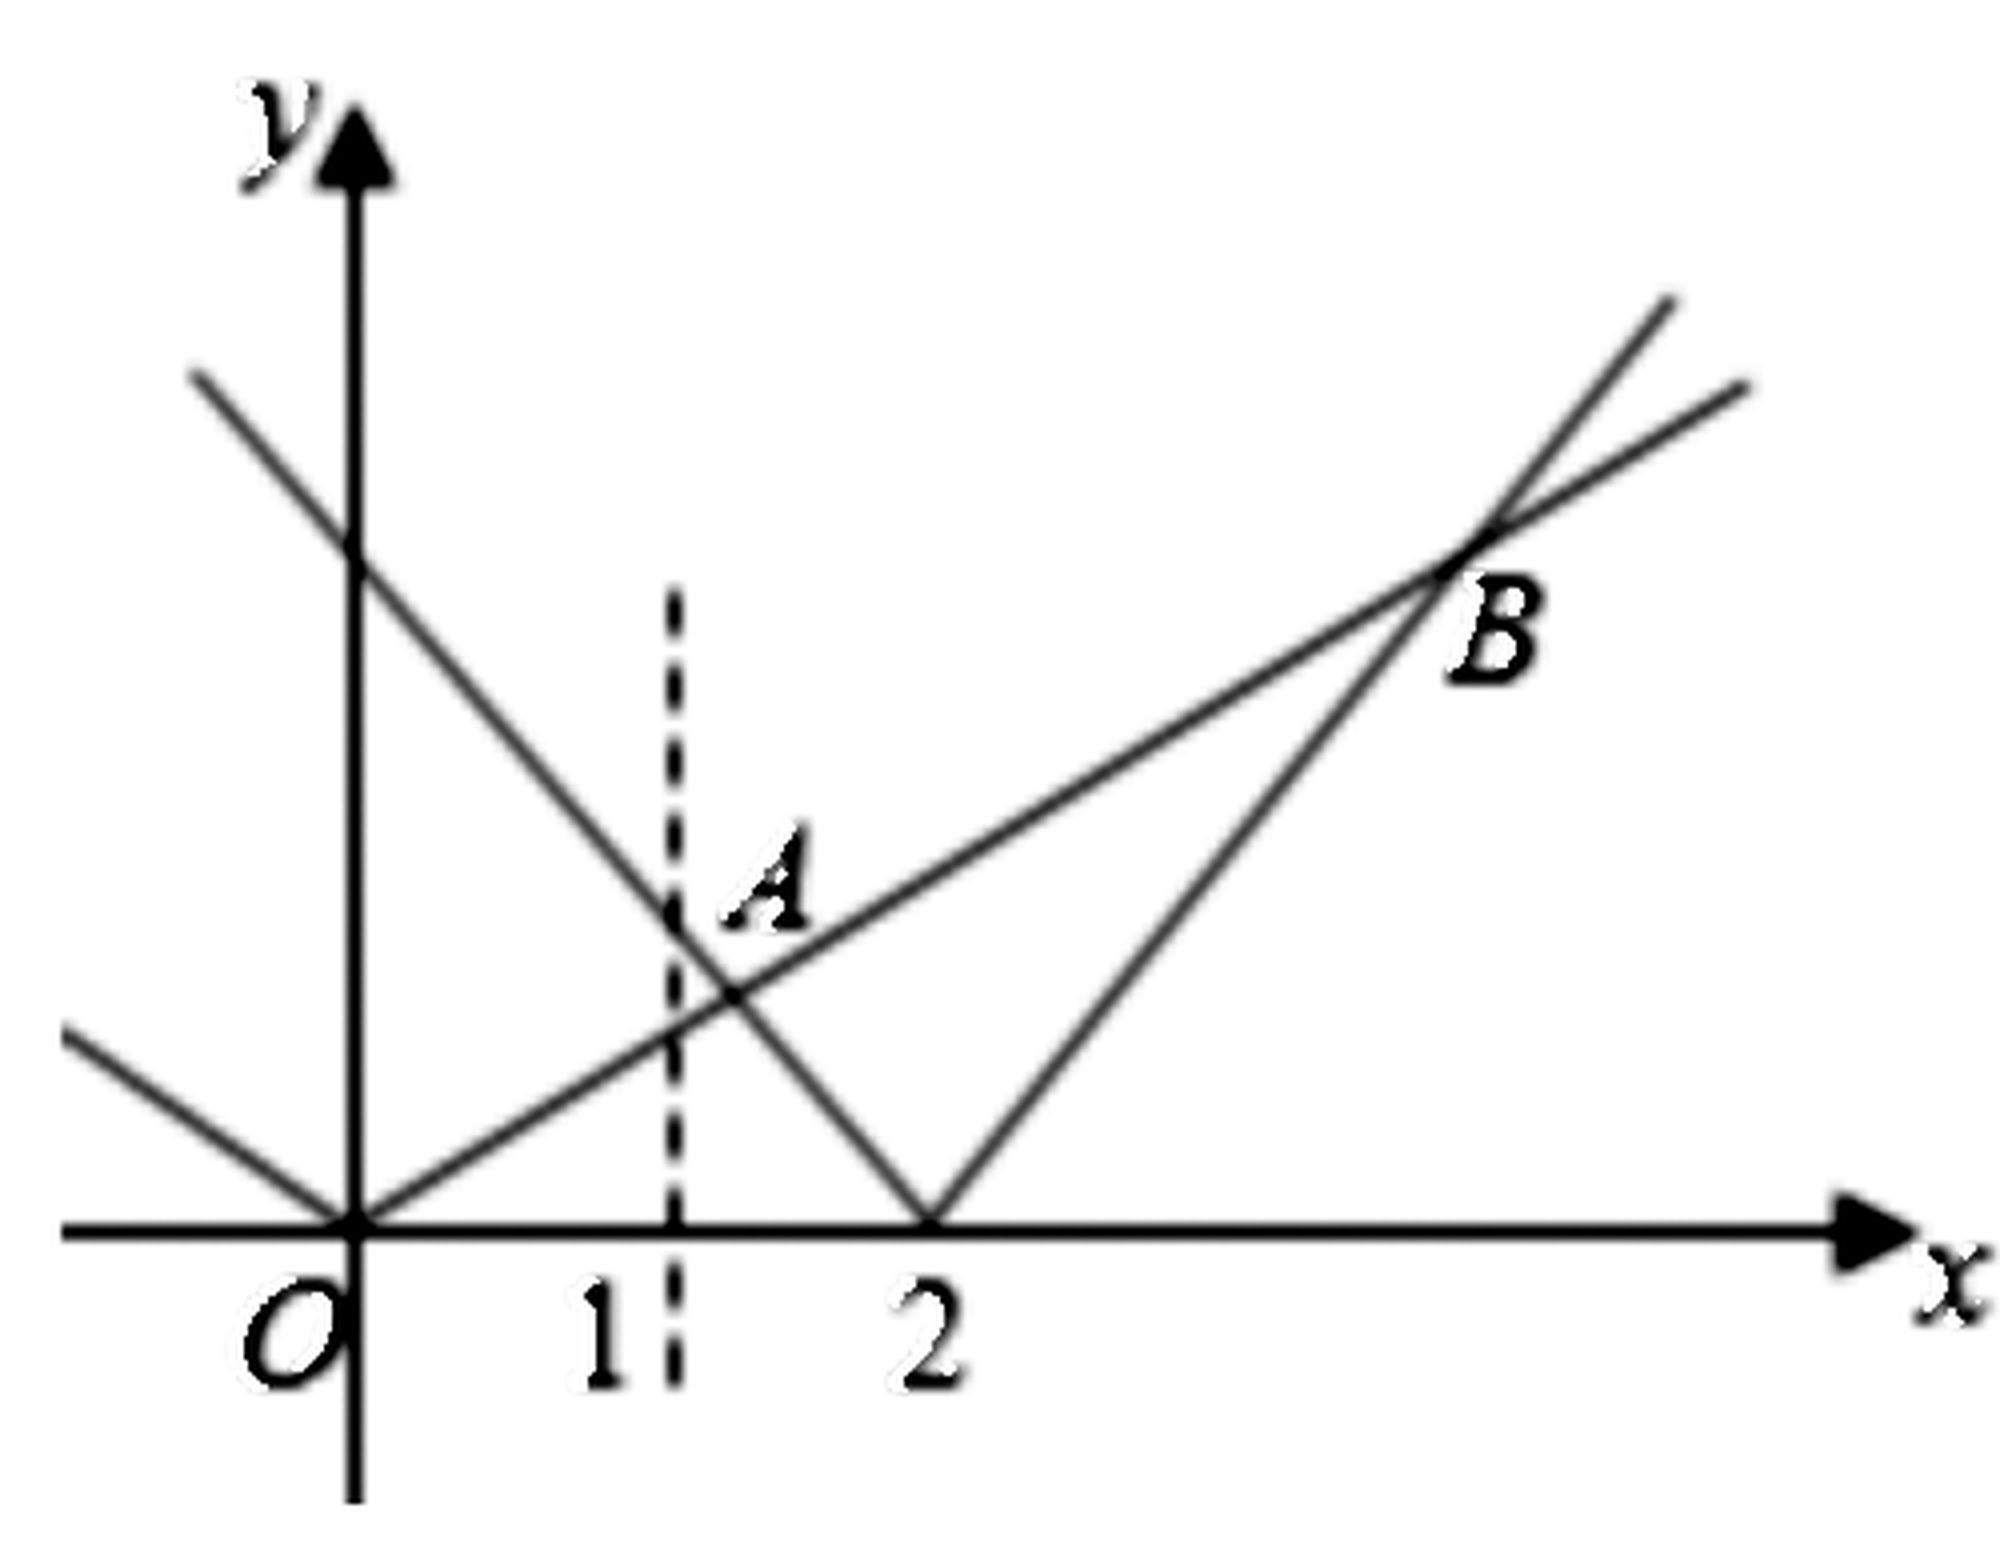
\includegraphics[width=0.40\textwidth]{figures/gao152_q15.png}
\end{center}
\step{由 $0<k<1$，得 $x_A>1$，}
\step{所以关于 $x$ 的不等式 $k\lvert x\rvert-\lvert x-2\rvert>0$ 恰好有 4 个整数解，是 2，3，4，5，}
\step{由 $\begin{cases}y=kx\\y=x-2\end{cases}\Rightarrow x_B=\dfrac2{1-k}\in(5,6]$，故 $\dfrac35<k\leqslant\dfrac23$；故选 $B$.}
\solend
\fi

% === Q16 === 咖啡优惠题；解析 12 行（跨 04 页上下半）；故选 C
\item 上海是全球咖啡店最多的城市. 若某品牌的某种在售咖啡产品价格为 30 元/杯，其原材料成本为 7 元/杯，营销成本为 5 元/杯，且该品牌门店提供如下 4 种优惠方式：(1) 首杯免单，每人限用一次；(2) 3.8 折优惠券，每人限用一次；(3) 买 2 杯送 2 杯，每人限用两次；(4) 买 5 杯送 5 杯，不限使用人数和使用次数. 每位消费者都可以在以上 4 种优惠方式中选择不多于 2 种使用. 现在某个公司有 5 位后勤工作人员去该品牌门店帮每位技术人员购买 1 杯咖啡，购买杯数与技术人员人数须保持一致；请问，这个公司的技术人员不少于\mbox{（\quad）}人时，无论 5 位后勤人员采用什么样的优惠方式购买咖啡，这笔订单该品牌门店都能保证盈利.

\keepwithprev
A. 20\qquad\qquad B. 25\qquad\qquad C. 30\qquad\qquad D. 35

\ifanswer
\solbegin
\step{按各优惠不叠加于同一杯理解，3.8 折券仅用于一杯，}
\step{买赠中的购买杯按原价付款.}
\step{设共购 $n$ 杯，免单、券购、原价购买的杯数分别为 $a,b,c$，其中 $0\leqslant a,b\leqslant5$，}
\step{其余为买赠咖啡，每杯成本为 12 元，}
\step{利润为 $P=15(n-a-b-c)+11.4b+30c-12n=3n-15a-3.6b+15c$，}
\step{若 $a,b$ 不同时为 5，则 $15a+3.6b\leqslant75+14.4=89.4$，}
\step{当 $n\geqslant30$ 时，$P\geqslant90-89.4=0.6>0$.}
\step{若 $a=b=5$，则每人均已使用免单和优惠券两种方式，其余均须原价购买，}
\step{$P=57+30(n-10)-12n=18n-243\geqslant297>0$.}
\step{当 $n=29$ 时，4 人各用方式 (1)(2) 购得 2 杯，}
\step{另 1 人用方式 (1) 及两次方式 (4) 购得 21 杯，}
\step{此时 $P=4\times11.4+2\times150-29\times12=-2.4<0$，因此最小人数为 30，故选 $C$.}% $2\times150$ 为两次方式（4）各买 5 杯的付款，照录（见 ⑤ 3）
\solend
\fi

\end{enumerate}

\bigsec{三、解答题}

\begin{enumerate}
\setcounter{enumi}{16}

% === Q17 === 解集含 \R／\varnothing；解析 4 行
\item 若 $a$、$b\in\R$，求关于 $x$ 的不等式 $ax\geqslant b$ 的解集.

\ifanswer
\solbegin
\step{当 $a>0$ 时，原不等式的解集为 $\left\{x\mid x\geqslant\dfrac ba\right\}$；}
\step{当 $a<0$ 时，原不等式的解集为 $\left\{x\mid x\leqslant\dfrac ba\right\}$；}
\step{当 $a=0$，$b\leqslant0$ 时，原不等式的解集为 $\R$；}
\step{当 $a=0$，$b>0$ 时，原不等式的解集为 $\varnothing$.}
\solend
\fi

% === Q18 === 子集 ⊆ 两处照录；cases 块；解析 9 行（跨 05 页上下半）
\item 已知 $\alpha:x<3m-1$ 或 $x>-m$，$\beta:x<2$ 或 $x\geqslant4$.

(1) 若 $\alpha$ 是 $\beta$ 的充分条件，求实数 $m$ 的取值范围；

(2) 若 $\alpha$ 是 $\beta$ 的必要条件，求实数 $m$ 的取值范围.

\ifanswer
\solbegin
\step{(1) 设 $A=\{x\mid x<3m-1\text{ 或 }x>-m\}$，$B=\{x\mid x<2\text{ 或 }x\geqslant4\}$，}
\step{因为 $\alpha$ 是 $\beta$ 的充分条件，所以 $A\subseteq B$，}
\step{当 $3m-1>-m$ 时，即 $m>\dfrac14$，此时 $A=\R$，不满足题意；}
\step{当 $3m-1\leqslant-m$ 时，即 $m\leqslant\dfrac14$，有 $\begin{cases}3m-1\leqslant2\\-m\geqslant4\end{cases}$，解得 $m\leqslant-4$；}
\step{综上，$m$ 的取值范围为 $(-\infty,-4]$.}
\step{(2) 因为 $\alpha$ 是 $\beta$ 的必要条件，所以 $B\subseteq A$，}
\step{当 $3m-1>-m$ 时，即 $m>\dfrac14$，此时 $A=\R$，$B\subseteq A$ 成立；}
\step{当 $3m-1\leqslant-m$ 时，即 $m\leqslant\dfrac14$，有 $\begin{cases}3m-1\geqslant2\\-m<4\end{cases}$，无解.}
\step{综上，$m$ 的取值范围为 $\left[\dfrac14,+\infty\right)$.}
\solend
\fi

% === Q19 === \varnothing 空集照录；解析 9 行
\item 设关于 $x$ 的不等式 $x^2+4x+k-1\geqslant0$ 的解集为 $A$.

(1) 若 $A=\R$，求实数 $k$ 的取值范围；

(2) 求证：不存在实数 $k$，使得 $A=\varnothing$.

\ifanswer
\solbegin
\step{(1) 配方得 $x^2+4x+k-1=(x+2)^2+k-5$，}
\step{若 $A=\R$，取 $x=-2$，得 $k-5\geqslant0$，即 $k\geqslant5$.}
\step{当 $k\geqslant5$ 时，对任意 $x\in\R$，都有 $(x+2)^2+k-5\geqslant0$，因此 $A=\R$.}
\step{所以 $k$ 的取值范围为 $[5,+\infty)$.}
\step{(2) 当 $k\geqslant5$ 时，由 (1) 得 $A=\R\ne\varnothing$.}
\step{当 $k<5$ 时，取 $x_0=-2+\sqrt{5-k}$，}
\step{则 $x_0^2+4x_0+k-1=(x_0+2)^2+k-5=(5-k)+k-5=0$，}
\step{所以 $x_0\in A$，即 $A\ne\varnothing$.}
\step{因此，不存在实数 $k$，使得 $A=\varnothing$.}
\solend
\fi

% === Q20 === |A\cap B|=1 印等号；等腰偏高粗 \Delta 照录；解析 12 行（跨 06→07 页）
\item 设 $m\in\R$. 集合 $A=\left\{x\mid\dfrac{x^2+x}{x+1}\geqslant\dfrac{2x+m}{x},x\in\R\right\}$，
$B=\left\{x\mid\dfrac{x^2+x}{x+1}\leqslant\dfrac{2x+m}{x},x\in\R\right\}$.

(1) 若 $m=8$，记集合 $M=A\cap(0,+\infty)$，求集合 $M$；

(2) 用 $\lvert T\rvert$ 代表集合 $T$ 的元素个数. 若 $\lvert A\cap B\rvert=1$，记 $m$ 的取值集合为 $C$，试比较 $\lvert C\rvert$ 与 2 的大小，并证明你的结论.

\ifanswer
\solbegin
\step{(1) 当 $m=8$，$x>0$ 时，$\dfrac{x^2+x}{x+1}\geqslant\dfrac{2x+8}{x}\Leftrightarrow x^2-2x-8\geqslant0$}
\step{$\Leftrightarrow(x-4)(x+2)\geqslant0\Leftrightarrow x\geqslant4$，所以 $M=[4,+\infty)$.}
\step{(2) 原分式有意义须 $x\ne-1,0$，因此 $x\in A\cap B\Leftrightarrow\begin{cases}x^2-2x-m=0\\x\ne-1,0\end{cases}$，}
\step{方程的判别式为 $\Delta=4(1+m)$.}
\step{当 $m<-1$ 时，方程无实根，$\lvert A\cap B\rvert=0$；}
\step{当 $m=-1$ 时，方程只有一个实根 1，$A\cap B=\{1\}$.}
\step{当 $m>-1$ 时，方程有两个不同实根.}
\step{其中，0 为根当且仅当 $m=0$，$-1$ 为根当且仅当 $m=3$.}
\step{$m=0$ 时，方程的根为 $0,2$，$A\cap B=\{2\}$；}
\step{$m=3$ 时，方程的根为 $-1,3$，$A\cap B=\{3\}$.}
\step{$m>-1$ 且 $m\ne0,3$ 时，两个实根均满足原分式的定义条件，$\lvert A\cap B\rvert=2$.}
\step{因此 $C=\{-1,0,3\}$，$\lvert C\rvert=3>2$.}
\solend
\fi

% === Q21 === "性质 p"新定义、\Q 归一、M\subseteq\R 照录；解析 19 行（跨 07→08 页）
\item 设集合 $M\subseteq\R$. 若 $M$ 中元素个数大于等于 2，且 $M$ 的任意不同元素 $a$、$b$ 均满足 $a^3-\dfrac14b\in M$，则称集合 $M$ 具有“性质 $p$”.

(1) 试判断集合 $\Q$、集合 $\left\{-\dfrac{\sqrt3}{2},0,\dfrac{\sqrt3}{2}\right\}$ 是否具有“性质 $p$”，并说明理由；

(2) 设 $m$ 为大于等于 2 的正整数. 若集合 $A=\{x_1,x_2,\cdots,x_m\}$，且具有“性质 $p$”，求证：$m=2$，并求集合 $A$ 中所有元素的乘积.

\ifanswer
\solbegin
\step{(1) $\Q$ 中至少有两个元素，且任意不同的 $a,b\in\Q$ 均满足 $a^3-\dfrac14b\in\Q$，}
\step{故 $\Q$ 具有“性质 $p$”.}
\step{对于另一集合，取 $a=0$，$b=\dfrac{\sqrt3}{2}$，则 $a^3-\dfrac14b=-\dfrac{\sqrt3}{8}$ 不属于该集合，}
\step{故其不具有“性质 $p$”.}
\step{(2) 将 $A$ 中元素按 $x_1<x_2<\cdots<x_m$ 排列.}
\step{若 $m\geqslant3$，由性质 $p$ 及幂函数 $y=x^3$ 的单调性，}
\step{有 $x_1^3-\dfrac14x_m<\cdots<x_1^3-\dfrac14x_2<x_m^3-\dfrac14x_2<x_m^3-\dfrac14x_1$，}
\step{上述 $m+1$ 个互不相同的数均属于 $A$，与 $A$ 只有 $m$ 个元素矛盾，}
\step{因此 $m=2$.}
\step{设 $A=\{a,b\}$，$a<b$.}
\step{因为 $a^3-\dfrac14b<b^3-\dfrac14a$，且两者均属于 $A$，}
\step{所以 $a^3-\dfrac14b=a$，$b^3-\dfrac14a=b$，}
\step{两式相减并除以 $a-b\ne0$，}
\step{以及两式相加，分别得 $a^2+ab+b^2=\dfrac34$，$(a+b)(a^2-ab+b^2)=\dfrac54(a+b)$，}
\step{代入 $a^2-ab+b^2=\dfrac34-2ab$，得 $(a+b)(4ab+1)=0$，}
\step{若 $a+b=0$，则 $-ab=a^2+ab+b^2=\dfrac34$，即 $ab=-\dfrac34$；}
\step{若 $a+b\ne0$，则 $ab=-\dfrac14$.}
\step{分别取 $A=\left\{-\dfrac{\sqrt3}{2},\dfrac{\sqrt3}{2}\right\}$，$A=\left\{\dfrac{1-\sqrt3}{2\sqrt2},\dfrac{1+\sqrt3}{2\sqrt2}\right\}$，}
\step{代入均有 $a^3-\dfrac14b=a$、$b^3-\dfrac14a=b$，故两种乘积均可取得.}
\solend
\fi

\end{enumerate}

\end{document}
"
% 紧凑版：xelatex "\def\iscompact{1}% 高一152_位育中学_期中.tex
%   —— 高一上数学"2026-2027 年位育中学高一上期中"（试卷版/答案版/紧凑版）
% 试卷版：xelatex 高一152_位育中学_期中.tex
% 答案版：xelatex "\def\isanswer{1}% 高一152_位育中学_期中.tex
%   —— 高一上数学"2026-2027 年位育中学高一上期中"（试卷版/答案版/紧凑版）
% 试卷版：xelatex 高一152_位育中学_期中.tex
% 答案版：xelatex "\def\isanswer{1}% 高一152_位育中学_期中.tex
%   —— 高一上数学"2026-2027 年位育中学高一上期中"（试卷版/答案版/紧凑版）
% 试卷版：xelatex 高一152_位育中学_期中.tex
% 答案版：xelatex "\def\isanswer{1}\input{高一152_位育中学_期中.tex}"
% 紧凑版：xelatex "\def\iscompact{1}\input{高一152_位育中学_期中.tex}"
%
% ① 原始材料：微信公众号"魔都数学加油站"文章，连载"27学年高一152"，原文标题
% "27学年高一152——2026-2027年上海市位育中学高一上期中"；
% 原文链接：https://mp.weixin.qq.com/s/v4_G6oTX2BuPz9L-KtLRfw 。
% 正文为 8 张 PNG 页（01/03/05/06/07/08 为 2560×3620，02/04 为 4762×6735，
% 同一篇各页分辨率混排，逐页按各自分辨率裁图核对，别按预览比例换算裁框）。
% 体例：讲评版——填空 3—12（10 题）、选择 13—16（4 题）、解答 17—21（5 题），
% 共 19 题，自第 3 题起编；题目、答案、解析均据原图转录；卷面粉红色水印
% "魔都数学加油站"及公众号页脚未录入。
% 全卷插图清单（逐页通读 8 页确认）：1 幅——第 15 题解析配图（两条折线
% $y=k\lvert x\rvert$ 与 $y=\lvert x-2\rvert$ 及坐标图，03 页右下，含 O、1、2、
% A、B 与虚线 $x=1$），解析写"的图象如下"，仅答案版出，裁
% figures/gao152_q15.png（去粉水印、去色、4× LANCZOS 放大）。
%
% 卷首标题：原卷印作"2026-2027 年位育中学高一上期中"，年份区间按全稿惯例排 en dash；
% 原卷卷面未印副标题，本稿按同期中卷知识模块口径补出"集合与常用逻辑用语、不等式、函数"。
%
% ② 与原卷的排版差异：
%   ① 原文从第 3 题起，本稿保留原题号；共 19 题三节，解答题 5 题到 21；
%   ② 混合体例：第 3、5 题只印【答案】、无【解析】，按 高一140 第 5 题／
%      高一145 第 3 题成例另提 \ans{}、不补造解析；第 13、14 题把答案"D"
%      直接印在题干括号内、题下无【解析】，按 高一84／148／149 成例括号留空、
%      另提 \ans{$D$}；其余 15 题印【解析】、用 \solbegin…\solend；
%      第 15、16 题答案在解析末句"故选 B／C"、括号留空、不另提 \ans{}；
%      答案版【答案】/【解析】标记数 = 19 = 全卷题数（4 个 \ans ＋ 15 个 \solbegin）；
%   ③ 原卷卷面未印副标题，本稿按知识模块口径补出；
%   ④ 原卷填空横线按全稿惯例排 \blankline[4.4em]；选择题括号排 \mbox{（\quad）}、
%      四道选择题的选项段前按惯例各加 \keepwithprev；解答题不留作答区、不加
%      \anspace（原卷为讲评版，109—113 起全稿不用 \anspace）；
%   ⑤ 数集黑板粗体：Q7"全集为 R"、Q9"$\lVert PQ\rVert$ 定义"无数集、
%      Q12"$t\in Z$"、Q13"$k\in Z$ 与 $=\R$"、Q17"$a,b\in R$"、Q19"$A=\R$"、
%      Q20"$m\in\R$"、Q21"$M\subseteq\R$ 与集合 $\Q$"原卷印正体粗体或黑板体
%      R/Q/Z，按全稿惯例归一 \R／\Q／\Z；绝对值排 \lvert…\rvert
%      （Q4、Q9、Q11、Q15），集合描述竖线排 \mid（Q7、Q13、Q20、Q21），
%      距离双竖线排 \lVert…\rVert（Q9 与题干、解析的 ||PQ||／||AB||）；
%      不等号按全稿惯例排 \leqslant／\geqslant；补集照原卷上划线排 \overline{A}
%      （Q7 题干＋解析）；空集 \varnothing（Q17、Q19）；
%      子集 Q18 两处、Q21 题干一处均印带下划线 ⊆、照录 \subseteq（见 ④），
%      本卷无单线 \subset 用例；
%   ⑥ 判别式 Δ/△ 两形混用逐处照录、不得统一：Q11 解析"判别式 △=k²−8k>0"
%      印扁等边细线三角、照录 \triangle，Q20 (2) 解析"判别式为 Δ=4(1+m)"
%      印等腰偏高粗三角、照录 \Delta（/tmp/gao152/z/zoom/q11_delta.png、
%      q20_delta.png 放大并与 151 卷同型并排比较）；
%   ⑦ 中文弯引号照录：Q11"长度"、Q21"性质 p"（题干、两问与解析多处）、
%      Q6 从">"、"<"、"≥"、"≤"中选符号、Q16"（1）…（4）"半角括号；
%      注释里一律 ASCII 引号；数学式内 CJK 用 \text{}（Q13 的"或／且"、
%      Q18 集合描述的"或"）；
%   ⑧ "图像／图象"：全卷仅 Q15 解析一处"的图象如下"，印"图象"（象，无亻）、
%      照录；其余各题无"图像"字样。子题标号 (1)(2)(3)(4) 半角括号照录；
%   ⑨ 半角逗号在数学组之间是全稿惯例、非笔误，逐处照录（Q6、Q10、Q16、
%      Q20、Q21 的 $a,b,c$ 之类）；行末西文句点 ASCII `.`；
%      行中全角逗号／顿号照录（Q11"（a,b）"、Q16"7 元/杯"、Q21"$\Q$、集合"）；
%   ⑩ 复杂式照录别简化：Q4 四组 cases 块（整体各占一个印刷行）、Q8
%      $\frac{x_0}{e^{x_0}}=\frac13$、Q10 $4a^2+b^2=4$、Q12 $b=\frac2a$、
%      Q16 利润式 $P=15(n-a-b-c)+11.4b+30c-12n$、Q18 cases 块、
%      Q20 分式 $\frac{x^2+x}{x+1}$、Q21 $a^3-\frac14b$ 与两组取值集合；
%      \left…\right 不得拆到不同 $…$ 组（Q4 cases 前的 \left\{ 一律改
%      \begin{cases}…\end{cases}、Q17 $\left\{x\mid x\ge\frac ba\right\}$、
%      Q20 $\left\{x\mid\cdots\right\}$、Q21 $\left\{-\frac{\sqrt3}2,\ldots\right\}$）；
%   ⑪ 一条 \step = 原卷解析的一个印刷行，cases 块整体算一个印刷行；别并折行、
%      别拆行。Q12 七行、Q16 十二行、Q18 九行、Q19 九行、Q20 十二行、
%      Q21 十九行均按印刷行逐条断，不丢行；
%   ⑫ 配图：Q15 解析配图（仅答案版出）放 \ifanswer 内 \solbegin…\solend 的
%      \step 之间（高一73 第 16 题／高一150 Q12 成例）；题干无配图，故无
%      \needvspace；
%   ⑬ 原卷解析内无红色"法一／法二"之类小标题，故本卷无 \stepm；红色水印
%      "魔都数学加油站"不录入；
%   ⑭ 跨页续印按题合并：见 ⑥；
%
% ③ 行数复核：一条 \step = 原卷解析的一个印刷行，cases 块作一个印刷行计。
%   逐题数（主会话逐页核对定稿）：Q3：0（只印【答案】、提 \ans{}）；Q4：2；
%   Q5：0（只印【答案】、提 \ans{}）；Q6：1；Q7：1；Q8：1；Q9：1；
%   Q10：4；Q11：5；Q12：7；Q13：0（答案印括号内、提 \ans{}）；
%   Q14：0（答案印括号内、提 \ans{}）；Q15：4；Q16：12；Q17：4；
%   Q18：9；Q19：9；Q20：12；Q21：19。
%   合计 91 条 \step（本卷无 \stepm），与原卷逐题印刷行相等。全卷 15 题设
%   \solbegin…\solend ＋ Q3／Q5／Q13／Q14 四处 \ans{}，答案版
%   【答案】/【解析】标记数 = 19 = 全卷题数。
%
% ④ 判别式／子集符号结论（逐处放大原图照录、不得统一，主会话像素级复核）：
%   判别式：Q11 解析"方程 $x^2-kx+2k=0$ 的判别式 $\triangle=k^2-8k>0$"
%      印扁等边细线三角、照录 \triangle；Q20 (2) 解析"方程的判别式为
%      $\Delta=4(1+m)$"印等腰偏高粗三角、照录 \Delta
%      （/tmp/gao152/z/zoom/q11_delta.png、q20_delta.png；与 高一142／151
%      的"Δ/△ 混用逐处照录"口径一致）。本卷无几何三角形符号。
%   子集：Q18 解析 (1)"$A\subseteq B$"、(2)"$B\subseteq A$"与 Q21 题干
%      "$M\subseteq\R$"共 3 处均印带下划线 ⊆、照录 \subseteq
%      （/tmp/gao152/z/zoom/q18_subset.png、q21_subset.png 放大确认）；
%      本卷无单线 ⊂ 用例。补集上划线 \overline{A}（Q7）、空集 \varnothing
%      （Q17 解析末行、Q19 题干 (2) 与解析）、数集 \R／\Q／\Z 归一见 ② ⑤。
%
% ⑤ 存疑照录（放大原图确认，照录未改、正文对应处另有 % 注）：
%   1. Q11 题干"已知关于 $x$ 的不等式 $x^2-kx+2k<0$ 有实数解，且解集区间
%      长度不超过 3 个单位"，解析据 $\lvert x_1-x_2\rvert\leqslant3$ 推；
%      判别式用扁三角 \triangle（见 ④），照录未改。
%   2. Q12 解析"$t=-1$ 时取 $b=\frac2a\in[-2,-1]$，$c=-1$，则 $ab+c=2-1=1$"
%      ——$b$ 径写 $\frac2a$（无负号），放大 03 页确认，照录未改。
%   3. Q16 解析"$P=4\times11.4+2\times150-29\times12=-2.4<0$"中的
%      $2\times150$ 为两次方式（4）各买 5 杯的付款，照录未改。
%   4. Q20 (2) 题干"若 $\lvert A\cap B\rvert=1$"印等号（非 $\leqslant1$），
%      放大 06 页 /tmp/gao152/z/zoom/q20_eq1.png 确认，照录未改。
%   5. Q21 题干"性质 p"用弯引号且 $p$ 为斜体小写，逐处照录未统一；
%      解析 (2) 末两组 $A$ 的取值集合照录未简化。
%   6. "图像／图象"仅 Q15 一处"图象"、Δ/△ 两形并用（Q11 \triangle、
%      Q20 \Delta）均逐处照录、未统一（见 ② ⑥ ⑧ 与 ④）。
%   全卷除此 6 类外未发现其它笔误／自相矛盾处；19 题中 15 题印【解析】、
%   Q3／Q5 只印【答案】、Q13／Q14 答案印题干括号内（见 ② ②）。
%
% ⑥ 跨页续印按题合并说明（逐页核实定稿）：Q3—Q5 题干＋【答案】／【解析】
%   在 01 页上半，Q6—Q8 题干＋解析在 01 页下半；Q9、Q10 题干＋解析、
%   Q11 题干＋解析、Q12 题干＋解析首行在 02 页；Q12 解析余 6 行续 03 页
%   上半，"二、选择题"标题与 Q13 题干＋选项在 03 页下半；Q13 选项 C／D、
%   Q14 题干＋四选项＋（无解析）、Q15 题干＋四选项＋解析前 3 行＋配图在
%   03 页下半，Q15 解析末行（由 cases 求 $x_B$）续 04 页顶；Q16 题干＋四选项
%   ＋解析前 5 行在 04 页上半，解析余 7 行在 04 页下半；"三、解答题"标题与
%   Q17 题干＋解析首行在 04 页末，Q17 解析余 3 行、Q18 题干＋两问＋解析首
%   4 行在 05 页上半，Q18 解析余 5 行在 05 页下半；Q19 题干＋两问＋解析
%   (1) 4 行在 05—06 页（(2) 题干续 06 页顶），解析 (2) 5 行在 06 页上半；
%   Q20 题干＋两问＋解析 (1) 2 行＋(2) 首行在 06 页下半；Q20 (2) 解析余
%   9 行、Q21 题干＋两问＋解析 (1) 4 行在 07 页；Q21 (2) 解析 19 行中前
%   6 行在 07—08 页上半、末 13 行续 08 页下半，末行"故两种乘积均可取得"
%   为全卷收尾（08 页下半仅水印、无其它正文）。
%   本稿按题连排，不丢行、不并折行；全卷末题为第 21 题，无附加题节。
%
\documentclass[a4paper,11pt]{article}
\usepackage{common}

\begin{document}

\examtitlest[3]{2026--2027 年位育中学高一上期中}{集合与常用逻辑用语、不等式、函数}

\bigsec{一、填空题}

\begin{enumerate}
\setcounter{enumi}{2}

% === Q3 === 原卷只印【答案】、无【解析】，另提 \ans{}，不补造解析
\item 设 $x>0$. 若 $\ln x=-1$，则 $x=$\blankline[4.4em].

\ifanswer
\ans{$\dfrac1{\mathrm{e}}$}
\fi

% === Q4 === 四组 cases 块同一印刷行；解析 2 行
\item 不等式 $\lvert 1-2x\rvert>x$ 的解集为\blankline[4.4em].

\ifanswer
\solbegin
\step{不等式 $\lvert 1-2x\rvert>x$ 即为 $\begin{cases}1-2x\geqslant0\\1-2x>x\end{cases}$ 或 $\begin{cases}1-2x<0\\2x-1>x\end{cases}$，即 $\begin{cases}x\leqslant\frac12\\x<\frac13\end{cases}$ 或 $\begin{cases}x>\frac12\\x>1\end{cases}$，}
\step{则有 $x<\dfrac13$ 或 $x>1$，则解集为 $\left(-\infty,\dfrac13\right)\cup(1,+\infty)$.}
\solend
\fi

% === Q5 === 原卷只印【答案】、无【解析】；\frac1x\ge1 印单线 ≥，按全稿惯例 \geqslant
\item 不等式 $\dfrac1x\geqslant1$ 的解集为\blankline[4.4em].

\ifanswer
\ans{$(0,1]$}
\fi

% === Q6 === 从四个符号中选一个，中文弯引号照录；解析 1 行
\item 设 $a$、$b>0$，则 $a^2+b^2$\blankline[4.4em]$2(2a-b)-5$（从“$>$”、“$<$”、“$\geqslant$”、“$\leqslant$”中选择一个符号填写）.

\ifanswer
\solbegin
\step{$a^2+b^2-[2(2a-b)-5]=(a-2)^2+(b+1)^2>0$，故 $a^2+b^2>2(2a-b)-5$.}
\solend
\fi

% === Q7 === 补集上划线 \overline{A}；集合描述竖线 \mid；解析 1 行
\item 已知全集为 $\R$，集合 $A=\{x\mid y=\sqrt{x-2}\}$，集合 $B=\{y\mid y=\sqrt{x-2}\}$，则 $\overline{A}\cap B=$\blankline[4.4em].

\ifanswer
\solbegin
\step{$A=[2,+\infty)$，$B=[0,+\infty)$，所以 $\overline{A}\cap B=[0,2)$.}
\solend
\fi

% === Q8 === \frac{x_0}{e^{x_0}}=\frac13 照录；解析 1 行
\item 设正数 $x_0$ 满足等式 $\dfrac{x_0}{e^{x_0}}=\dfrac13$，则 $x_0-\ln x_0=$\blankline[4.4em].

\ifanswer
\solbegin
\step{等式两边取自然对数，得 $\ln x_0-x_0=-\ln3$，即 $x_0-\ln x_0=\ln3$.}
\solend
\fi

% === Q9 === 距离双竖线 \lVert…\rVert；解析 1 行
\item 在平面直角坐标系 $xOy$ 中，设点 $P(x_1,y_1)$，$Q(x_2,y_2)$，定义：$\lVert PQ\rVert=\lvert x_1-x_2\rvert+\lvert y_1-y_2\rvert$. 若点 $A(1,0)$，点 $B$ 为直线 $y=x+2$ 上的动点，则 $\lVert AB\rVert$ 的最小值为\blankline[4.4em].

\ifanswer
\solbegin
\step{$\lVert AB\rVert=\lvert x-1\rvert+\lvert y\rvert=\lvert x-1\rvert+\lvert x+2\rvert\geqslant3$，最小值为 3.}
\solend
\fi

% === Q10 === 解析 4 行
\item 已知 $a$、$b$ 均为正数，且 $a^2+\dfrac14b^2=1$，则 $a\sqrt{1+b^2}$ 的最大值为\blankline[4.4em].

\ifanswer
\solbegin
\step{因为 $a$、$b$ 均为正数，且 $a^2+\dfrac14b^2=1$，所以 $4a^2+b^2=4$，}
\step{所以 $a\sqrt{1+b^2}=\dfrac12\cdot2a\cdot\sqrt{1+b^2}\leqslant\dfrac12\cdot\dfrac{4a^2+1+b^2}{2}=\dfrac54$，}
\step{当且仅当 $4a^2=b^2+1$ 即 $a=\dfrac{\sqrt{10}}4$，$b=\dfrac{\sqrt6}2$ 时取等号，}
\step{故 $a\sqrt{1+b^2}$ 的最大值为 $\dfrac54$.}
\solend
\fi

% === Q11 === 扁等边细线判别式 \triangle 照录（见 ④）；"长度"弯引号；解析 5 行
\item 一般地，把 $b-a$ 称为区间 $(a,b)$ 的“长度”. 已知关于 $x$ 的不等式 $x^2-kx+2k<0$ 有实数解，且解集区间长度不超过 3 个单位，则实数 $k$ 的取值范围是\blankline[4.4em].

\ifanswer
\solbegin
\step{因为不等式 $x^2-kx+2k<0$ 有解，}
\step{所以方程 $x^2-kx+2k=0$ 的判别式 $\triangle=k^2-8k>0$，解得 $k>8$ 或 $k<0$，}
\step{由 $x_1+x_2=k$，$x_1x_2=2k$，得 $(x_1-x_2)^2=(x_1+x_2)^2-4x_1x_2=k^2-8k$，}
\step{由 $\lvert x_1-x_2\rvert\leqslant3$，得 $(x_1-x_2)^2\leqslant9$，即 $k^2-8k\leqslant9$，解得 $-1\leqslant k\leqslant9$，}
\step{所以 $-1\leqslant k<0$ 或 $8<k\leqslant9$，即实数 $k$ 的取值范围是 $[-1,0)\cup(8,9]$.}
\solend
\fi

% === Q12 === $b=\frac2a$ 无负号、$c=-1$ 照录（见 ⑤ 2）；解析 7 行（跨 02→03 页）
\item 设 $t\in\Z$，且对任意 $a\in[-2,t]$，总存在 $b,c\in[-2,t]$，使得 $ab+c=1$，则 $t$ 的所有取值为\blankline[4.4em].

\ifanswer
\solbegin
\step{$[-2,t]$ 是区间，要求 $t>-2$，故 $t\geqslant-1$.}
\step{当 $t\geqslant1$ 时，对任意 $a\in[-2,t]$，}
\step{取 $b=0$，$c=1$，两者都属于 $[-2,t]$，且 $ab+c=1$.}
\step{当 $t=0$ 时，取 $a=0$，则 $c=1\notin[-2,0]$，不成立.}
\step{当 $t=-1$ 时，对任意 $a\in[-2,-1]$，取 $b=\dfrac2a\in[-2,-1]$，$c=-1$，}% 原卷径写 $b=\frac2a$（无负号），放大 03 页确认，照录未改（见 ⑤ 2）
\step{则 $ab+c=2-1=1$.}
\step{所以 $t=-1$ 或 $t\geqslant1$（$t\in\Z$）.}
\solend
\fi

\end{enumerate}

\bigsec{二、选择题}

\begin{enumerate}
\setcounter{enumi}{12}

% === Q13 === 答案 D 印在题干括号内、无【解析】，按 高一84／148／149 成例括号留空、另提 \ans{}
\item 下列说法错误的是\mbox{（\quad）}

\keepwithprev
A. 奇数集可以表示为 $\{x\mid x=2k+1,k\in\Z\}$

B. 奇数集可以表示为 $\{x\mid x=2k-1,k\in\Z\}$

C. $\{x\mid x\ne2\text{ 或 }x\ne-2\}=\R$

D. $\{x\mid x\ne2\text{ 且 }x\ne-2\}=\R$

\ifanswer
\ans{$D$}
\fi

% === Q14 === 答案 D 印在题干括号内、无【解析】；选项两行两列
\item 设 $a$、$b$、$c>0$，且 $a\ne1$，则以下代数式中，不恒成立的是\mbox{（\quad）}

\keepwithprev
A. $\log_a 1=0$\qquad\qquad B. $a^{\log_a b}=b$

C. $\log_a b+\log_a c=\log_a(bc)$\qquad\qquad D. $\log_a b=\dfrac1{\log_b a}$

\ifanswer
\ans{$D$}
\fi

% === Q15 === "图象"（象，无亻）照录；解析配图仅答案版出；答案在解析末句故选 B
\item 若关于 $x$ 的不等式 $k\lvert x\rvert>\lvert x-2\rvert$ 恰好有 4 个整数解，则实数 $k$ 的取值范围是\mbox{（\quad）}

\keepwithprev
A. $\left(\dfrac35,\dfrac23\right)$\qquad B. $\left(\dfrac35,\dfrac23\right]$\qquad C. $\left(\dfrac35,1\right)$\qquad D. $\left(\dfrac35,1\right]$

\ifanswer
\solbegin
\step{由题意得 $0<k<1$，函数 $y=k\lvert x\rvert$ 与 $y=\lvert x-2\rvert$ 的图象如下，}
\begin{center}
% 两条折线坐标图取 03 页右下，去粉色水印、去色、4× LANCZOS 放大；仅答案版出
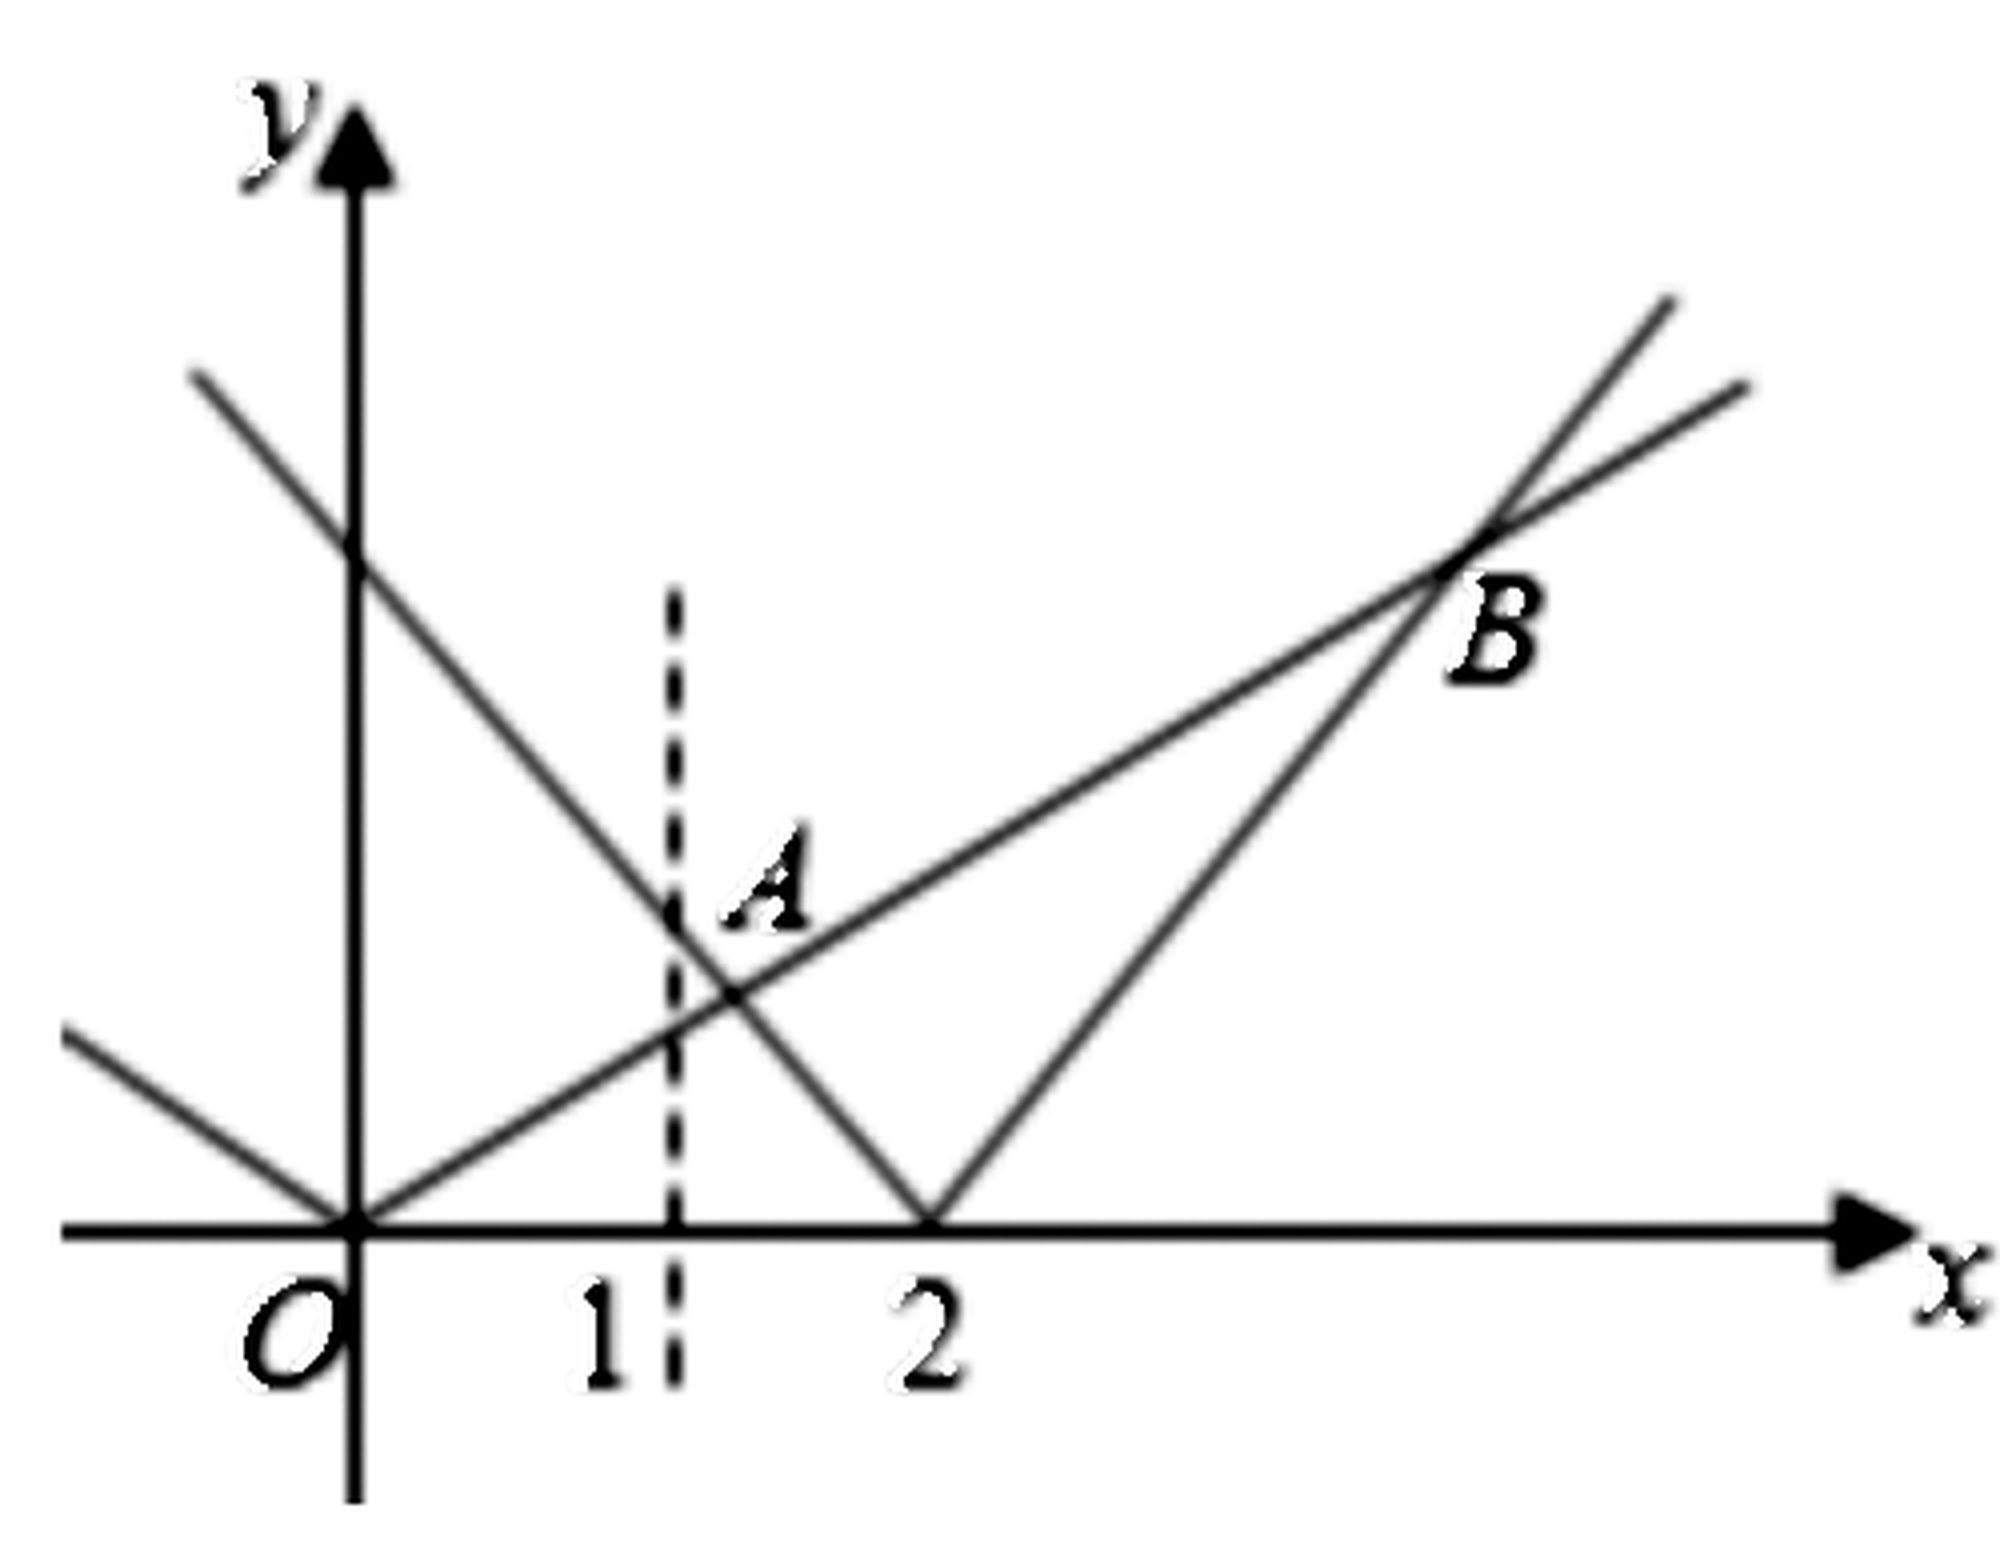
\includegraphics[width=0.40\textwidth]{figures/gao152_q15.png}
\end{center}
\step{由 $0<k<1$，得 $x_A>1$，}
\step{所以关于 $x$ 的不等式 $k\lvert x\rvert-\lvert x-2\rvert>0$ 恰好有 4 个整数解，是 2，3，4，5，}
\step{由 $\begin{cases}y=kx\\y=x-2\end{cases}\Rightarrow x_B=\dfrac2{1-k}\in(5,6]$，故 $\dfrac35<k\leqslant\dfrac23$；故选 $B$.}
\solend
\fi

% === Q16 === 咖啡优惠题；解析 12 行（跨 04 页上下半）；故选 C
\item 上海是全球咖啡店最多的城市. 若某品牌的某种在售咖啡产品价格为 30 元/杯，其原材料成本为 7 元/杯，营销成本为 5 元/杯，且该品牌门店提供如下 4 种优惠方式：(1) 首杯免单，每人限用一次；(2) 3.8 折优惠券，每人限用一次；(3) 买 2 杯送 2 杯，每人限用两次；(4) 买 5 杯送 5 杯，不限使用人数和使用次数. 每位消费者都可以在以上 4 种优惠方式中选择不多于 2 种使用. 现在某个公司有 5 位后勤工作人员去该品牌门店帮每位技术人员购买 1 杯咖啡，购买杯数与技术人员人数须保持一致；请问，这个公司的技术人员不少于\mbox{（\quad）}人时，无论 5 位后勤人员采用什么样的优惠方式购买咖啡，这笔订单该品牌门店都能保证盈利.

\keepwithprev
A. 20\qquad\qquad B. 25\qquad\qquad C. 30\qquad\qquad D. 35

\ifanswer
\solbegin
\step{按各优惠不叠加于同一杯理解，3.8 折券仅用于一杯，}
\step{买赠中的购买杯按原价付款.}
\step{设共购 $n$ 杯，免单、券购、原价购买的杯数分别为 $a,b,c$，其中 $0\leqslant a,b\leqslant5$，}
\step{其余为买赠咖啡，每杯成本为 12 元，}
\step{利润为 $P=15(n-a-b-c)+11.4b+30c-12n=3n-15a-3.6b+15c$，}
\step{若 $a,b$ 不同时为 5，则 $15a+3.6b\leqslant75+14.4=89.4$，}
\step{当 $n\geqslant30$ 时，$P\geqslant90-89.4=0.6>0$.}
\step{若 $a=b=5$，则每人均已使用免单和优惠券两种方式，其余均须原价购买，}
\step{$P=57+30(n-10)-12n=18n-243\geqslant297>0$.}
\step{当 $n=29$ 时，4 人各用方式 (1)(2) 购得 2 杯，}
\step{另 1 人用方式 (1) 及两次方式 (4) 购得 21 杯，}
\step{此时 $P=4\times11.4+2\times150-29\times12=-2.4<0$，因此最小人数为 30，故选 $C$.}% $2\times150$ 为两次方式（4）各买 5 杯的付款，照录（见 ⑤ 3）
\solend
\fi

\end{enumerate}

\bigsec{三、解答题}

\begin{enumerate}
\setcounter{enumi}{16}

% === Q17 === 解集含 \R／\varnothing；解析 4 行
\item 若 $a$、$b\in\R$，求关于 $x$ 的不等式 $ax\geqslant b$ 的解集.

\ifanswer
\solbegin
\step{当 $a>0$ 时，原不等式的解集为 $\left\{x\mid x\geqslant\dfrac ba\right\}$；}
\step{当 $a<0$ 时，原不等式的解集为 $\left\{x\mid x\leqslant\dfrac ba\right\}$；}
\step{当 $a=0$，$b\leqslant0$ 时，原不等式的解集为 $\R$；}
\step{当 $a=0$，$b>0$ 时，原不等式的解集为 $\varnothing$.}
\solend
\fi

% === Q18 === 子集 ⊆ 两处照录；cases 块；解析 9 行（跨 05 页上下半）
\item 已知 $\alpha:x<3m-1$ 或 $x>-m$，$\beta:x<2$ 或 $x\geqslant4$.

(1) 若 $\alpha$ 是 $\beta$ 的充分条件，求实数 $m$ 的取值范围；

(2) 若 $\alpha$ 是 $\beta$ 的必要条件，求实数 $m$ 的取值范围.

\ifanswer
\solbegin
\step{(1) 设 $A=\{x\mid x<3m-1\text{ 或 }x>-m\}$，$B=\{x\mid x<2\text{ 或 }x\geqslant4\}$，}
\step{因为 $\alpha$ 是 $\beta$ 的充分条件，所以 $A\subseteq B$，}
\step{当 $3m-1>-m$ 时，即 $m>\dfrac14$，此时 $A=\R$，不满足题意；}
\step{当 $3m-1\leqslant-m$ 时，即 $m\leqslant\dfrac14$，有 $\begin{cases}3m-1\leqslant2\\-m\geqslant4\end{cases}$，解得 $m\leqslant-4$；}
\step{综上，$m$ 的取值范围为 $(-\infty,-4]$.}
\step{(2) 因为 $\alpha$ 是 $\beta$ 的必要条件，所以 $B\subseteq A$，}
\step{当 $3m-1>-m$ 时，即 $m>\dfrac14$，此时 $A=\R$，$B\subseteq A$ 成立；}
\step{当 $3m-1\leqslant-m$ 时，即 $m\leqslant\dfrac14$，有 $\begin{cases}3m-1\geqslant2\\-m<4\end{cases}$，无解.}
\step{综上，$m$ 的取值范围为 $\left[\dfrac14,+\infty\right)$.}
\solend
\fi

% === Q19 === \varnothing 空集照录；解析 9 行
\item 设关于 $x$ 的不等式 $x^2+4x+k-1\geqslant0$ 的解集为 $A$.

(1) 若 $A=\R$，求实数 $k$ 的取值范围；

(2) 求证：不存在实数 $k$，使得 $A=\varnothing$.

\ifanswer
\solbegin
\step{(1) 配方得 $x^2+4x+k-1=(x+2)^2+k-5$，}
\step{若 $A=\R$，取 $x=-2$，得 $k-5\geqslant0$，即 $k\geqslant5$.}
\step{当 $k\geqslant5$ 时，对任意 $x\in\R$，都有 $(x+2)^2+k-5\geqslant0$，因此 $A=\R$.}
\step{所以 $k$ 的取值范围为 $[5,+\infty)$.}
\step{(2) 当 $k\geqslant5$ 时，由 (1) 得 $A=\R\ne\varnothing$.}
\step{当 $k<5$ 时，取 $x_0=-2+\sqrt{5-k}$，}
\step{则 $x_0^2+4x_0+k-1=(x_0+2)^2+k-5=(5-k)+k-5=0$，}
\step{所以 $x_0\in A$，即 $A\ne\varnothing$.}
\step{因此，不存在实数 $k$，使得 $A=\varnothing$.}
\solend
\fi

% === Q20 === |A\cap B|=1 印等号；等腰偏高粗 \Delta 照录；解析 12 行（跨 06→07 页）
\item 设 $m\in\R$. 集合 $A=\left\{x\mid\dfrac{x^2+x}{x+1}\geqslant\dfrac{2x+m}{x},x\in\R\right\}$，
$B=\left\{x\mid\dfrac{x^2+x}{x+1}\leqslant\dfrac{2x+m}{x},x\in\R\right\}$.

(1) 若 $m=8$，记集合 $M=A\cap(0,+\infty)$，求集合 $M$；

(2) 用 $\lvert T\rvert$ 代表集合 $T$ 的元素个数. 若 $\lvert A\cap B\rvert=1$，记 $m$ 的取值集合为 $C$，试比较 $\lvert C\rvert$ 与 2 的大小，并证明你的结论.

\ifanswer
\solbegin
\step{(1) 当 $m=8$，$x>0$ 时，$\dfrac{x^2+x}{x+1}\geqslant\dfrac{2x+8}{x}\Leftrightarrow x^2-2x-8\geqslant0$}
\step{$\Leftrightarrow(x-4)(x+2)\geqslant0\Leftrightarrow x\geqslant4$，所以 $M=[4,+\infty)$.}
\step{(2) 原分式有意义须 $x\ne-1,0$，因此 $x\in A\cap B\Leftrightarrow\begin{cases}x^2-2x-m=0\\x\ne-1,0\end{cases}$，}
\step{方程的判别式为 $\Delta=4(1+m)$.}
\step{当 $m<-1$ 时，方程无实根，$\lvert A\cap B\rvert=0$；}
\step{当 $m=-1$ 时，方程只有一个实根 1，$A\cap B=\{1\}$.}
\step{当 $m>-1$ 时，方程有两个不同实根.}
\step{其中，0 为根当且仅当 $m=0$，$-1$ 为根当且仅当 $m=3$.}
\step{$m=0$ 时，方程的根为 $0,2$，$A\cap B=\{2\}$；}
\step{$m=3$ 时，方程的根为 $-1,3$，$A\cap B=\{3\}$.}
\step{$m>-1$ 且 $m\ne0,3$ 时，两个实根均满足原分式的定义条件，$\lvert A\cap B\rvert=2$.}
\step{因此 $C=\{-1,0,3\}$，$\lvert C\rvert=3>2$.}
\solend
\fi

% === Q21 === "性质 p"新定义、\Q 归一、M\subseteq\R 照录；解析 19 行（跨 07→08 页）
\item 设集合 $M\subseteq\R$. 若 $M$ 中元素个数大于等于 2，且 $M$ 的任意不同元素 $a$、$b$ 均满足 $a^3-\dfrac14b\in M$，则称集合 $M$ 具有“性质 $p$”.

(1) 试判断集合 $\Q$、集合 $\left\{-\dfrac{\sqrt3}{2},0,\dfrac{\sqrt3}{2}\right\}$ 是否具有“性质 $p$”，并说明理由；

(2) 设 $m$ 为大于等于 2 的正整数. 若集合 $A=\{x_1,x_2,\cdots,x_m\}$，且具有“性质 $p$”，求证：$m=2$，并求集合 $A$ 中所有元素的乘积.

\ifanswer
\solbegin
\step{(1) $\Q$ 中至少有两个元素，且任意不同的 $a,b\in\Q$ 均满足 $a^3-\dfrac14b\in\Q$，}
\step{故 $\Q$ 具有“性质 $p$”.}
\step{对于另一集合，取 $a=0$，$b=\dfrac{\sqrt3}{2}$，则 $a^3-\dfrac14b=-\dfrac{\sqrt3}{8}$ 不属于该集合，}
\step{故其不具有“性质 $p$”.}
\step{(2) 将 $A$ 中元素按 $x_1<x_2<\cdots<x_m$ 排列.}
\step{若 $m\geqslant3$，由性质 $p$ 及幂函数 $y=x^3$ 的单调性，}
\step{有 $x_1^3-\dfrac14x_m<\cdots<x_1^3-\dfrac14x_2<x_m^3-\dfrac14x_2<x_m^3-\dfrac14x_1$，}
\step{上述 $m+1$ 个互不相同的数均属于 $A$，与 $A$ 只有 $m$ 个元素矛盾，}
\step{因此 $m=2$.}
\step{设 $A=\{a,b\}$，$a<b$.}
\step{因为 $a^3-\dfrac14b<b^3-\dfrac14a$，且两者均属于 $A$，}
\step{所以 $a^3-\dfrac14b=a$，$b^3-\dfrac14a=b$，}
\step{两式相减并除以 $a-b\ne0$，}
\step{以及两式相加，分别得 $a^2+ab+b^2=\dfrac34$，$(a+b)(a^2-ab+b^2)=\dfrac54(a+b)$，}
\step{代入 $a^2-ab+b^2=\dfrac34-2ab$，得 $(a+b)(4ab+1)=0$，}
\step{若 $a+b=0$，则 $-ab=a^2+ab+b^2=\dfrac34$，即 $ab=-\dfrac34$；}
\step{若 $a+b\ne0$，则 $ab=-\dfrac14$.}
\step{分别取 $A=\left\{-\dfrac{\sqrt3}{2},\dfrac{\sqrt3}{2}\right\}$，$A=\left\{\dfrac{1-\sqrt3}{2\sqrt2},\dfrac{1+\sqrt3}{2\sqrt2}\right\}$，}
\step{代入均有 $a^3-\dfrac14b=a$、$b^3-\dfrac14a=b$，故两种乘积均可取得.}
\solend
\fi

\end{enumerate}

\end{document}
"
% 紧凑版：xelatex "\def\iscompact{1}% 高一152_位育中学_期中.tex
%   —— 高一上数学"2026-2027 年位育中学高一上期中"（试卷版/答案版/紧凑版）
% 试卷版：xelatex 高一152_位育中学_期中.tex
% 答案版：xelatex "\def\isanswer{1}\input{高一152_位育中学_期中.tex}"
% 紧凑版：xelatex "\def\iscompact{1}\input{高一152_位育中学_期中.tex}"
%
% ① 原始材料：微信公众号"魔都数学加油站"文章，连载"27学年高一152"，原文标题
% "27学年高一152——2026-2027年上海市位育中学高一上期中"；
% 原文链接：https://mp.weixin.qq.com/s/v4_G6oTX2BuPz9L-KtLRfw 。
% 正文为 8 张 PNG 页（01/03/05/06/07/08 为 2560×3620，02/04 为 4762×6735，
% 同一篇各页分辨率混排，逐页按各自分辨率裁图核对，别按预览比例换算裁框）。
% 体例：讲评版——填空 3—12（10 题）、选择 13—16（4 题）、解答 17—21（5 题），
% 共 19 题，自第 3 题起编；题目、答案、解析均据原图转录；卷面粉红色水印
% "魔都数学加油站"及公众号页脚未录入。
% 全卷插图清单（逐页通读 8 页确认）：1 幅——第 15 题解析配图（两条折线
% $y=k\lvert x\rvert$ 与 $y=\lvert x-2\rvert$ 及坐标图，03 页右下，含 O、1、2、
% A、B 与虚线 $x=1$），解析写"的图象如下"，仅答案版出，裁
% figures/gao152_q15.png（去粉水印、去色、4× LANCZOS 放大）。
%
% 卷首标题：原卷印作"2026-2027 年位育中学高一上期中"，年份区间按全稿惯例排 en dash；
% 原卷卷面未印副标题，本稿按同期中卷知识模块口径补出"集合与常用逻辑用语、不等式、函数"。
%
% ② 与原卷的排版差异：
%   ① 原文从第 3 题起，本稿保留原题号；共 19 题三节，解答题 5 题到 21；
%   ② 混合体例：第 3、5 题只印【答案】、无【解析】，按 高一140 第 5 题／
%      高一145 第 3 题成例另提 \ans{}、不补造解析；第 13、14 题把答案"D"
%      直接印在题干括号内、题下无【解析】，按 高一84／148／149 成例括号留空、
%      另提 \ans{$D$}；其余 15 题印【解析】、用 \solbegin…\solend；
%      第 15、16 题答案在解析末句"故选 B／C"、括号留空、不另提 \ans{}；
%      答案版【答案】/【解析】标记数 = 19 = 全卷题数（4 个 \ans ＋ 15 个 \solbegin）；
%   ③ 原卷卷面未印副标题，本稿按知识模块口径补出；
%   ④ 原卷填空横线按全稿惯例排 \blankline[4.4em]；选择题括号排 \mbox{（\quad）}、
%      四道选择题的选项段前按惯例各加 \keepwithprev；解答题不留作答区、不加
%      \anspace（原卷为讲评版，109—113 起全稿不用 \anspace）；
%   ⑤ 数集黑板粗体：Q7"全集为 R"、Q9"$\lVert PQ\rVert$ 定义"无数集、
%      Q12"$t\in Z$"、Q13"$k\in Z$ 与 $=\R$"、Q17"$a,b\in R$"、Q19"$A=\R$"、
%      Q20"$m\in\R$"、Q21"$M\subseteq\R$ 与集合 $\Q$"原卷印正体粗体或黑板体
%      R/Q/Z，按全稿惯例归一 \R／\Q／\Z；绝对值排 \lvert…\rvert
%      （Q4、Q9、Q11、Q15），集合描述竖线排 \mid（Q7、Q13、Q20、Q21），
%      距离双竖线排 \lVert…\rVert（Q9 与题干、解析的 ||PQ||／||AB||）；
%      不等号按全稿惯例排 \leqslant／\geqslant；补集照原卷上划线排 \overline{A}
%      （Q7 题干＋解析）；空集 \varnothing（Q17、Q19）；
%      子集 Q18 两处、Q21 题干一处均印带下划线 ⊆、照录 \subseteq（见 ④），
%      本卷无单线 \subset 用例；
%   ⑥ 判别式 Δ/△ 两形混用逐处照录、不得统一：Q11 解析"判别式 △=k²−8k>0"
%      印扁等边细线三角、照录 \triangle，Q20 (2) 解析"判别式为 Δ=4(1+m)"
%      印等腰偏高粗三角、照录 \Delta（/tmp/gao152/z/zoom/q11_delta.png、
%      q20_delta.png 放大并与 151 卷同型并排比较）；
%   ⑦ 中文弯引号照录：Q11"长度"、Q21"性质 p"（题干、两问与解析多处）、
%      Q6 从">"、"<"、"≥"、"≤"中选符号、Q16"（1）…（4）"半角括号；
%      注释里一律 ASCII 引号；数学式内 CJK 用 \text{}（Q13 的"或／且"、
%      Q18 集合描述的"或"）；
%   ⑧ "图像／图象"：全卷仅 Q15 解析一处"的图象如下"，印"图象"（象，无亻）、
%      照录；其余各题无"图像"字样。子题标号 (1)(2)(3)(4) 半角括号照录；
%   ⑨ 半角逗号在数学组之间是全稿惯例、非笔误，逐处照录（Q6、Q10、Q16、
%      Q20、Q21 的 $a,b,c$ 之类）；行末西文句点 ASCII `.`；
%      行中全角逗号／顿号照录（Q11"（a,b）"、Q16"7 元/杯"、Q21"$\Q$、集合"）；
%   ⑩ 复杂式照录别简化：Q4 四组 cases 块（整体各占一个印刷行）、Q8
%      $\frac{x_0}{e^{x_0}}=\frac13$、Q10 $4a^2+b^2=4$、Q12 $b=\frac2a$、
%      Q16 利润式 $P=15(n-a-b-c)+11.4b+30c-12n$、Q18 cases 块、
%      Q20 分式 $\frac{x^2+x}{x+1}$、Q21 $a^3-\frac14b$ 与两组取值集合；
%      \left…\right 不得拆到不同 $…$ 组（Q4 cases 前的 \left\{ 一律改
%      \begin{cases}…\end{cases}、Q17 $\left\{x\mid x\ge\frac ba\right\}$、
%      Q20 $\left\{x\mid\cdots\right\}$、Q21 $\left\{-\frac{\sqrt3}2,\ldots\right\}$）；
%   ⑪ 一条 \step = 原卷解析的一个印刷行，cases 块整体算一个印刷行；别并折行、
%      别拆行。Q12 七行、Q16 十二行、Q18 九行、Q19 九行、Q20 十二行、
%      Q21 十九行均按印刷行逐条断，不丢行；
%   ⑫ 配图：Q15 解析配图（仅答案版出）放 \ifanswer 内 \solbegin…\solend 的
%      \step 之间（高一73 第 16 题／高一150 Q12 成例）；题干无配图，故无
%      \needvspace；
%   ⑬ 原卷解析内无红色"法一／法二"之类小标题，故本卷无 \stepm；红色水印
%      "魔都数学加油站"不录入；
%   ⑭ 跨页续印按题合并：见 ⑥；
%
% ③ 行数复核：一条 \step = 原卷解析的一个印刷行，cases 块作一个印刷行计。
%   逐题数（主会话逐页核对定稿）：Q3：0（只印【答案】、提 \ans{}）；Q4：2；
%   Q5：0（只印【答案】、提 \ans{}）；Q6：1；Q7：1；Q8：1；Q9：1；
%   Q10：4；Q11：5；Q12：7；Q13：0（答案印括号内、提 \ans{}）；
%   Q14：0（答案印括号内、提 \ans{}）；Q15：4；Q16：12；Q17：4；
%   Q18：9；Q19：9；Q20：12；Q21：19。
%   合计 91 条 \step（本卷无 \stepm），与原卷逐题印刷行相等。全卷 15 题设
%   \solbegin…\solend ＋ Q3／Q5／Q13／Q14 四处 \ans{}，答案版
%   【答案】/【解析】标记数 = 19 = 全卷题数。
%
% ④ 判别式／子集符号结论（逐处放大原图照录、不得统一，主会话像素级复核）：
%   判别式：Q11 解析"方程 $x^2-kx+2k=0$ 的判别式 $\triangle=k^2-8k>0$"
%      印扁等边细线三角、照录 \triangle；Q20 (2) 解析"方程的判别式为
%      $\Delta=4(1+m)$"印等腰偏高粗三角、照录 \Delta
%      （/tmp/gao152/z/zoom/q11_delta.png、q20_delta.png；与 高一142／151
%      的"Δ/△ 混用逐处照录"口径一致）。本卷无几何三角形符号。
%   子集：Q18 解析 (1)"$A\subseteq B$"、(2)"$B\subseteq A$"与 Q21 题干
%      "$M\subseteq\R$"共 3 处均印带下划线 ⊆、照录 \subseteq
%      （/tmp/gao152/z/zoom/q18_subset.png、q21_subset.png 放大确认）；
%      本卷无单线 ⊂ 用例。补集上划线 \overline{A}（Q7）、空集 \varnothing
%      （Q17 解析末行、Q19 题干 (2) 与解析）、数集 \R／\Q／\Z 归一见 ② ⑤。
%
% ⑤ 存疑照录（放大原图确认，照录未改、正文对应处另有 % 注）：
%   1. Q11 题干"已知关于 $x$ 的不等式 $x^2-kx+2k<0$ 有实数解，且解集区间
%      长度不超过 3 个单位"，解析据 $\lvert x_1-x_2\rvert\leqslant3$ 推；
%      判别式用扁三角 \triangle（见 ④），照录未改。
%   2. Q12 解析"$t=-1$ 时取 $b=\frac2a\in[-2,-1]$，$c=-1$，则 $ab+c=2-1=1$"
%      ——$b$ 径写 $\frac2a$（无负号），放大 03 页确认，照录未改。
%   3. Q16 解析"$P=4\times11.4+2\times150-29\times12=-2.4<0$"中的
%      $2\times150$ 为两次方式（4）各买 5 杯的付款，照录未改。
%   4. Q20 (2) 题干"若 $\lvert A\cap B\rvert=1$"印等号（非 $\leqslant1$），
%      放大 06 页 /tmp/gao152/z/zoom/q20_eq1.png 确认，照录未改。
%   5. Q21 题干"性质 p"用弯引号且 $p$ 为斜体小写，逐处照录未统一；
%      解析 (2) 末两组 $A$ 的取值集合照录未简化。
%   6. "图像／图象"仅 Q15 一处"图象"、Δ/△ 两形并用（Q11 \triangle、
%      Q20 \Delta）均逐处照录、未统一（见 ② ⑥ ⑧ 与 ④）。
%   全卷除此 6 类外未发现其它笔误／自相矛盾处；19 题中 15 题印【解析】、
%   Q3／Q5 只印【答案】、Q13／Q14 答案印题干括号内（见 ② ②）。
%
% ⑥ 跨页续印按题合并说明（逐页核实定稿）：Q3—Q5 题干＋【答案】／【解析】
%   在 01 页上半，Q6—Q8 题干＋解析在 01 页下半；Q9、Q10 题干＋解析、
%   Q11 题干＋解析、Q12 题干＋解析首行在 02 页；Q12 解析余 6 行续 03 页
%   上半，"二、选择题"标题与 Q13 题干＋选项在 03 页下半；Q13 选项 C／D、
%   Q14 题干＋四选项＋（无解析）、Q15 题干＋四选项＋解析前 3 行＋配图在
%   03 页下半，Q15 解析末行（由 cases 求 $x_B$）续 04 页顶；Q16 题干＋四选项
%   ＋解析前 5 行在 04 页上半，解析余 7 行在 04 页下半；"三、解答题"标题与
%   Q17 题干＋解析首行在 04 页末，Q17 解析余 3 行、Q18 题干＋两问＋解析首
%   4 行在 05 页上半，Q18 解析余 5 行在 05 页下半；Q19 题干＋两问＋解析
%   (1) 4 行在 05—06 页（(2) 题干续 06 页顶），解析 (2) 5 行在 06 页上半；
%   Q20 题干＋两问＋解析 (1) 2 行＋(2) 首行在 06 页下半；Q20 (2) 解析余
%   9 行、Q21 题干＋两问＋解析 (1) 4 行在 07 页；Q21 (2) 解析 19 行中前
%   6 行在 07—08 页上半、末 13 行续 08 页下半，末行"故两种乘积均可取得"
%   为全卷收尾（08 页下半仅水印、无其它正文）。
%   本稿按题连排，不丢行、不并折行；全卷末题为第 21 题，无附加题节。
%
\documentclass[a4paper,11pt]{article}
\usepackage{common}

\begin{document}

\examtitlest[3]{2026--2027 年位育中学高一上期中}{集合与常用逻辑用语、不等式、函数}

\bigsec{一、填空题}

\begin{enumerate}
\setcounter{enumi}{2}

% === Q3 === 原卷只印【答案】、无【解析】，另提 \ans{}，不补造解析
\item 设 $x>0$. 若 $\ln x=-1$，则 $x=$\blankline[4.4em].

\ifanswer
\ans{$\dfrac1{\mathrm{e}}$}
\fi

% === Q4 === 四组 cases 块同一印刷行；解析 2 行
\item 不等式 $\lvert 1-2x\rvert>x$ 的解集为\blankline[4.4em].

\ifanswer
\solbegin
\step{不等式 $\lvert 1-2x\rvert>x$ 即为 $\begin{cases}1-2x\geqslant0\\1-2x>x\end{cases}$ 或 $\begin{cases}1-2x<0\\2x-1>x\end{cases}$，即 $\begin{cases}x\leqslant\frac12\\x<\frac13\end{cases}$ 或 $\begin{cases}x>\frac12\\x>1\end{cases}$，}
\step{则有 $x<\dfrac13$ 或 $x>1$，则解集为 $\left(-\infty,\dfrac13\right)\cup(1,+\infty)$.}
\solend
\fi

% === Q5 === 原卷只印【答案】、无【解析】；\frac1x\ge1 印单线 ≥，按全稿惯例 \geqslant
\item 不等式 $\dfrac1x\geqslant1$ 的解集为\blankline[4.4em].

\ifanswer
\ans{$(0,1]$}
\fi

% === Q6 === 从四个符号中选一个，中文弯引号照录；解析 1 行
\item 设 $a$、$b>0$，则 $a^2+b^2$\blankline[4.4em]$2(2a-b)-5$（从“$>$”、“$<$”、“$\geqslant$”、“$\leqslant$”中选择一个符号填写）.

\ifanswer
\solbegin
\step{$a^2+b^2-[2(2a-b)-5]=(a-2)^2+(b+1)^2>0$，故 $a^2+b^2>2(2a-b)-5$.}
\solend
\fi

% === Q7 === 补集上划线 \overline{A}；集合描述竖线 \mid；解析 1 行
\item 已知全集为 $\R$，集合 $A=\{x\mid y=\sqrt{x-2}\}$，集合 $B=\{y\mid y=\sqrt{x-2}\}$，则 $\overline{A}\cap B=$\blankline[4.4em].

\ifanswer
\solbegin
\step{$A=[2,+\infty)$，$B=[0,+\infty)$，所以 $\overline{A}\cap B=[0,2)$.}
\solend
\fi

% === Q8 === \frac{x_0}{e^{x_0}}=\frac13 照录；解析 1 行
\item 设正数 $x_0$ 满足等式 $\dfrac{x_0}{e^{x_0}}=\dfrac13$，则 $x_0-\ln x_0=$\blankline[4.4em].

\ifanswer
\solbegin
\step{等式两边取自然对数，得 $\ln x_0-x_0=-\ln3$，即 $x_0-\ln x_0=\ln3$.}
\solend
\fi

% === Q9 === 距离双竖线 \lVert…\rVert；解析 1 行
\item 在平面直角坐标系 $xOy$ 中，设点 $P(x_1,y_1)$，$Q(x_2,y_2)$，定义：$\lVert PQ\rVert=\lvert x_1-x_2\rvert+\lvert y_1-y_2\rvert$. 若点 $A(1,0)$，点 $B$ 为直线 $y=x+2$ 上的动点，则 $\lVert AB\rVert$ 的最小值为\blankline[4.4em].

\ifanswer
\solbegin
\step{$\lVert AB\rVert=\lvert x-1\rvert+\lvert y\rvert=\lvert x-1\rvert+\lvert x+2\rvert\geqslant3$，最小值为 3.}
\solend
\fi

% === Q10 === 解析 4 行
\item 已知 $a$、$b$ 均为正数，且 $a^2+\dfrac14b^2=1$，则 $a\sqrt{1+b^2}$ 的最大值为\blankline[4.4em].

\ifanswer
\solbegin
\step{因为 $a$、$b$ 均为正数，且 $a^2+\dfrac14b^2=1$，所以 $4a^2+b^2=4$，}
\step{所以 $a\sqrt{1+b^2}=\dfrac12\cdot2a\cdot\sqrt{1+b^2}\leqslant\dfrac12\cdot\dfrac{4a^2+1+b^2}{2}=\dfrac54$，}
\step{当且仅当 $4a^2=b^2+1$ 即 $a=\dfrac{\sqrt{10}}4$，$b=\dfrac{\sqrt6}2$ 时取等号，}
\step{故 $a\sqrt{1+b^2}$ 的最大值为 $\dfrac54$.}
\solend
\fi

% === Q11 === 扁等边细线判别式 \triangle 照录（见 ④）；"长度"弯引号；解析 5 行
\item 一般地，把 $b-a$ 称为区间 $(a,b)$ 的“长度”. 已知关于 $x$ 的不等式 $x^2-kx+2k<0$ 有实数解，且解集区间长度不超过 3 个单位，则实数 $k$ 的取值范围是\blankline[4.4em].

\ifanswer
\solbegin
\step{因为不等式 $x^2-kx+2k<0$ 有解，}
\step{所以方程 $x^2-kx+2k=0$ 的判别式 $\triangle=k^2-8k>0$，解得 $k>8$ 或 $k<0$，}
\step{由 $x_1+x_2=k$，$x_1x_2=2k$，得 $(x_1-x_2)^2=(x_1+x_2)^2-4x_1x_2=k^2-8k$，}
\step{由 $\lvert x_1-x_2\rvert\leqslant3$，得 $(x_1-x_2)^2\leqslant9$，即 $k^2-8k\leqslant9$，解得 $-1\leqslant k\leqslant9$，}
\step{所以 $-1\leqslant k<0$ 或 $8<k\leqslant9$，即实数 $k$ 的取值范围是 $[-1,0)\cup(8,9]$.}
\solend
\fi

% === Q12 === $b=\frac2a$ 无负号、$c=-1$ 照录（见 ⑤ 2）；解析 7 行（跨 02→03 页）
\item 设 $t\in\Z$，且对任意 $a\in[-2,t]$，总存在 $b,c\in[-2,t]$，使得 $ab+c=1$，则 $t$ 的所有取值为\blankline[4.4em].

\ifanswer
\solbegin
\step{$[-2,t]$ 是区间，要求 $t>-2$，故 $t\geqslant-1$.}
\step{当 $t\geqslant1$ 时，对任意 $a\in[-2,t]$，}
\step{取 $b=0$，$c=1$，两者都属于 $[-2,t]$，且 $ab+c=1$.}
\step{当 $t=0$ 时，取 $a=0$，则 $c=1\notin[-2,0]$，不成立.}
\step{当 $t=-1$ 时，对任意 $a\in[-2,-1]$，取 $b=\dfrac2a\in[-2,-1]$，$c=-1$，}% 原卷径写 $b=\frac2a$（无负号），放大 03 页确认，照录未改（见 ⑤ 2）
\step{则 $ab+c=2-1=1$.}
\step{所以 $t=-1$ 或 $t\geqslant1$（$t\in\Z$）.}
\solend
\fi

\end{enumerate}

\bigsec{二、选择题}

\begin{enumerate}
\setcounter{enumi}{12}

% === Q13 === 答案 D 印在题干括号内、无【解析】，按 高一84／148／149 成例括号留空、另提 \ans{}
\item 下列说法错误的是\mbox{（\quad）}

\keepwithprev
A. 奇数集可以表示为 $\{x\mid x=2k+1,k\in\Z\}$

B. 奇数集可以表示为 $\{x\mid x=2k-1,k\in\Z\}$

C. $\{x\mid x\ne2\text{ 或 }x\ne-2\}=\R$

D. $\{x\mid x\ne2\text{ 且 }x\ne-2\}=\R$

\ifanswer
\ans{$D$}
\fi

% === Q14 === 答案 D 印在题干括号内、无【解析】；选项两行两列
\item 设 $a$、$b$、$c>0$，且 $a\ne1$，则以下代数式中，不恒成立的是\mbox{（\quad）}

\keepwithprev
A. $\log_a 1=0$\qquad\qquad B. $a^{\log_a b}=b$

C. $\log_a b+\log_a c=\log_a(bc)$\qquad\qquad D. $\log_a b=\dfrac1{\log_b a}$

\ifanswer
\ans{$D$}
\fi

% === Q15 === "图象"（象，无亻）照录；解析配图仅答案版出；答案在解析末句故选 B
\item 若关于 $x$ 的不等式 $k\lvert x\rvert>\lvert x-2\rvert$ 恰好有 4 个整数解，则实数 $k$ 的取值范围是\mbox{（\quad）}

\keepwithprev
A. $\left(\dfrac35,\dfrac23\right)$\qquad B. $\left(\dfrac35,\dfrac23\right]$\qquad C. $\left(\dfrac35,1\right)$\qquad D. $\left(\dfrac35,1\right]$

\ifanswer
\solbegin
\step{由题意得 $0<k<1$，函数 $y=k\lvert x\rvert$ 与 $y=\lvert x-2\rvert$ 的图象如下，}
\begin{center}
% 两条折线坐标图取 03 页右下，去粉色水印、去色、4× LANCZOS 放大；仅答案版出
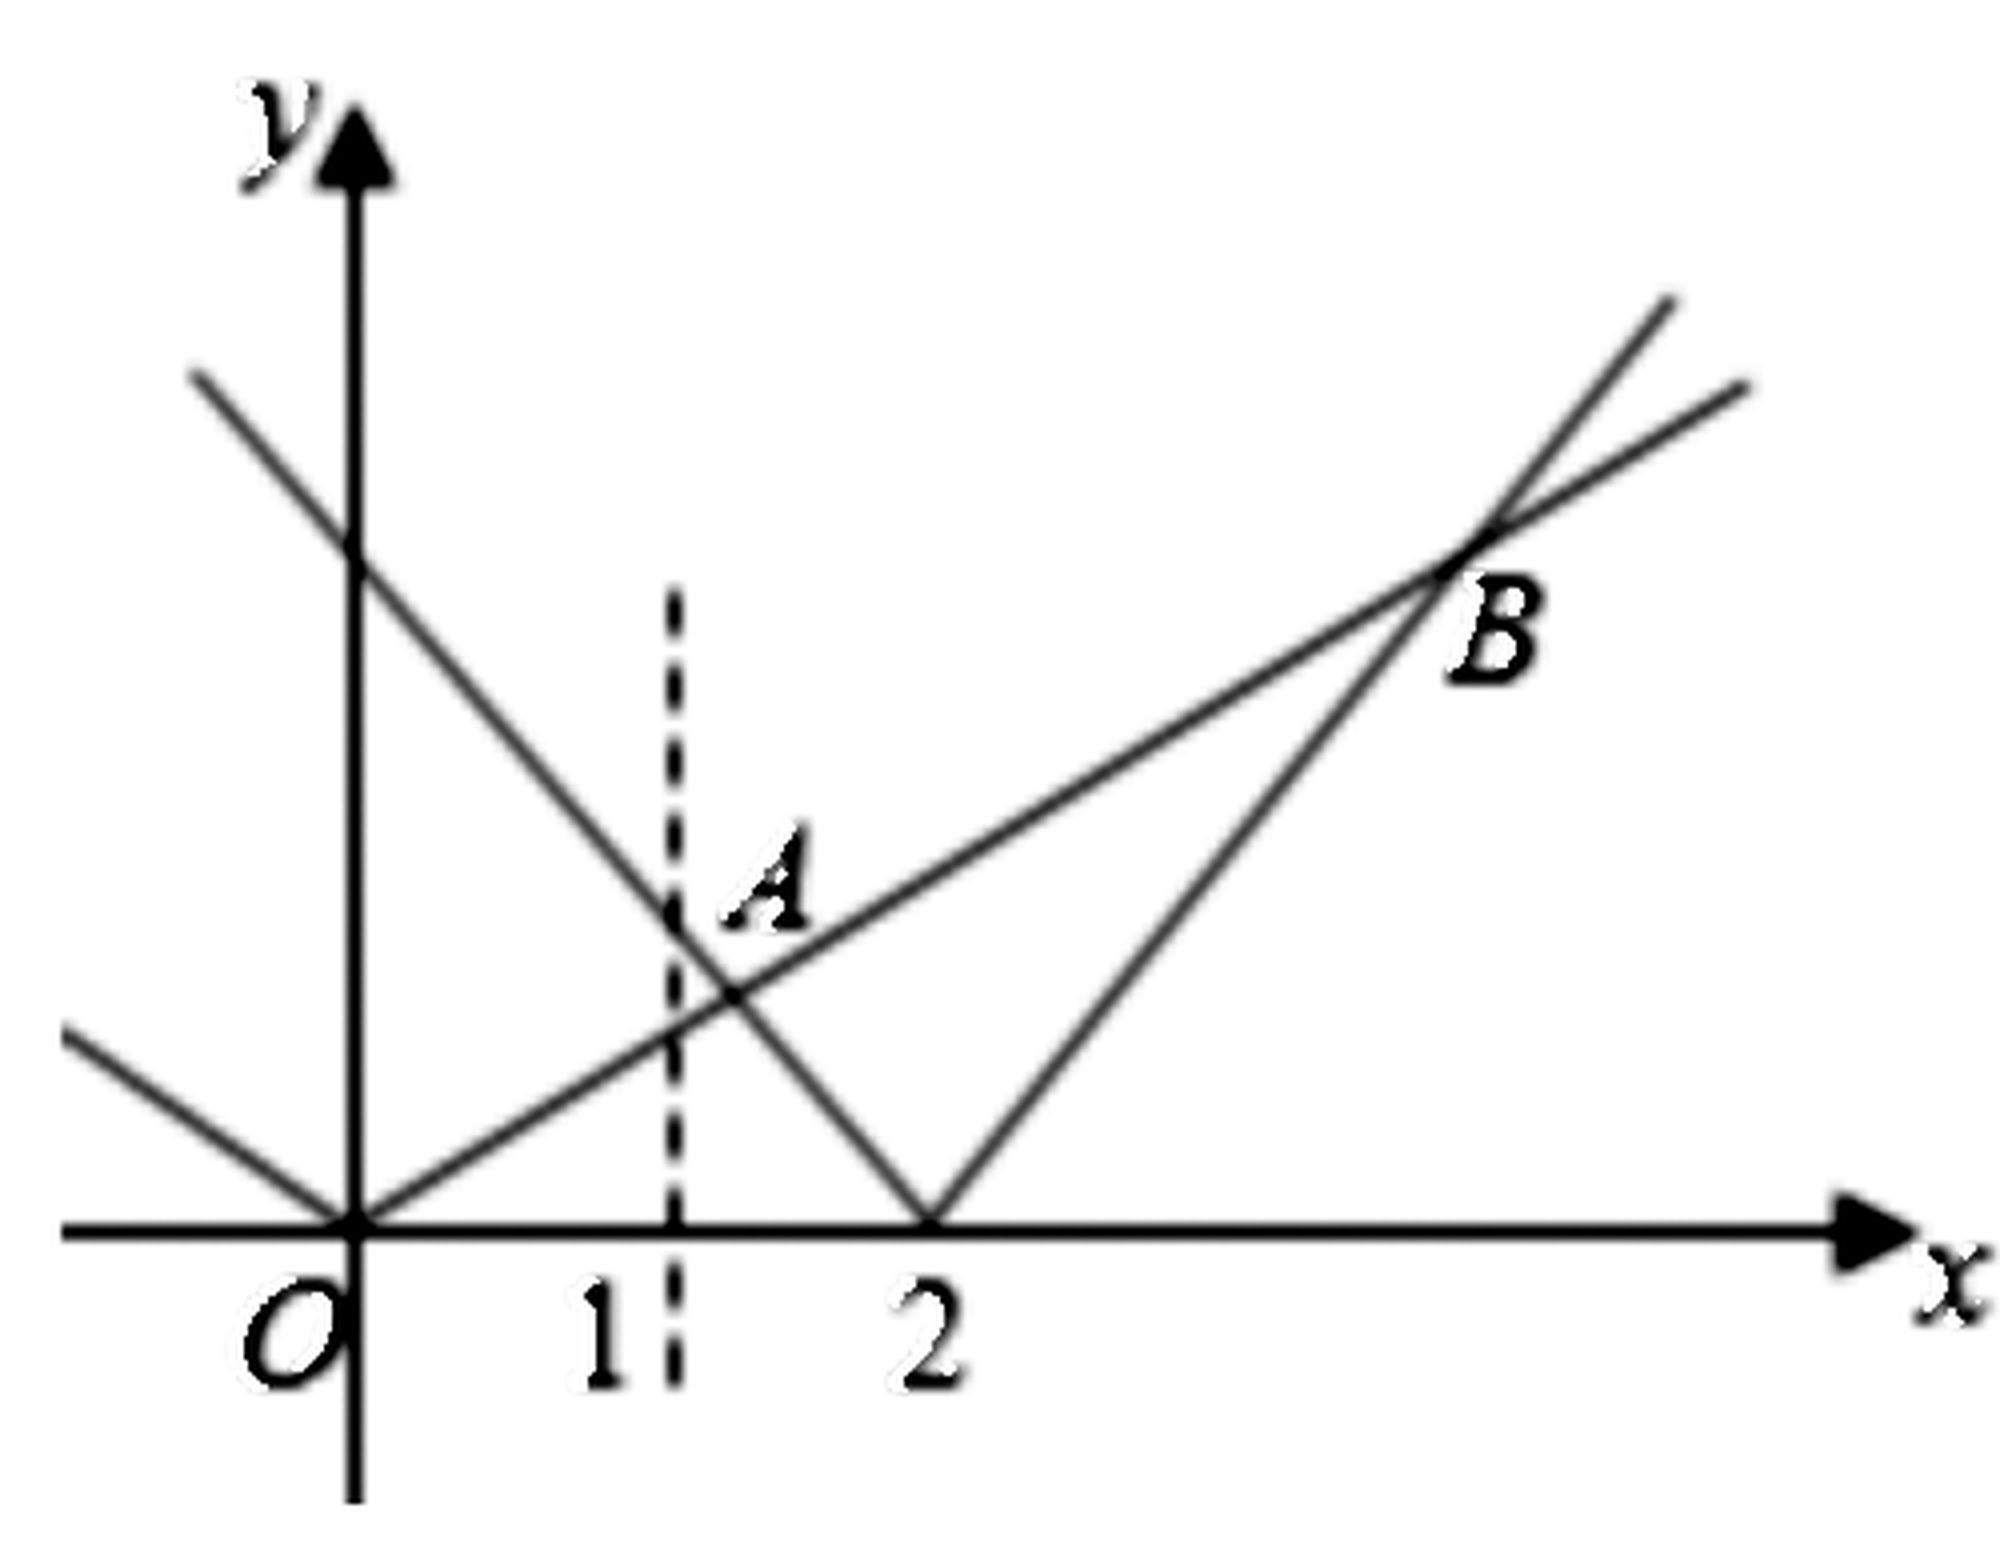
\includegraphics[width=0.40\textwidth]{figures/gao152_q15.png}
\end{center}
\step{由 $0<k<1$，得 $x_A>1$，}
\step{所以关于 $x$ 的不等式 $k\lvert x\rvert-\lvert x-2\rvert>0$ 恰好有 4 个整数解，是 2，3，4，5，}
\step{由 $\begin{cases}y=kx\\y=x-2\end{cases}\Rightarrow x_B=\dfrac2{1-k}\in(5,6]$，故 $\dfrac35<k\leqslant\dfrac23$；故选 $B$.}
\solend
\fi

% === Q16 === 咖啡优惠题；解析 12 行（跨 04 页上下半）；故选 C
\item 上海是全球咖啡店最多的城市. 若某品牌的某种在售咖啡产品价格为 30 元/杯，其原材料成本为 7 元/杯，营销成本为 5 元/杯，且该品牌门店提供如下 4 种优惠方式：(1) 首杯免单，每人限用一次；(2) 3.8 折优惠券，每人限用一次；(3) 买 2 杯送 2 杯，每人限用两次；(4) 买 5 杯送 5 杯，不限使用人数和使用次数. 每位消费者都可以在以上 4 种优惠方式中选择不多于 2 种使用. 现在某个公司有 5 位后勤工作人员去该品牌门店帮每位技术人员购买 1 杯咖啡，购买杯数与技术人员人数须保持一致；请问，这个公司的技术人员不少于\mbox{（\quad）}人时，无论 5 位后勤人员采用什么样的优惠方式购买咖啡，这笔订单该品牌门店都能保证盈利.

\keepwithprev
A. 20\qquad\qquad B. 25\qquad\qquad C. 30\qquad\qquad D. 35

\ifanswer
\solbegin
\step{按各优惠不叠加于同一杯理解，3.8 折券仅用于一杯，}
\step{买赠中的购买杯按原价付款.}
\step{设共购 $n$ 杯，免单、券购、原价购买的杯数分别为 $a,b,c$，其中 $0\leqslant a,b\leqslant5$，}
\step{其余为买赠咖啡，每杯成本为 12 元，}
\step{利润为 $P=15(n-a-b-c)+11.4b+30c-12n=3n-15a-3.6b+15c$，}
\step{若 $a,b$ 不同时为 5，则 $15a+3.6b\leqslant75+14.4=89.4$，}
\step{当 $n\geqslant30$ 时，$P\geqslant90-89.4=0.6>0$.}
\step{若 $a=b=5$，则每人均已使用免单和优惠券两种方式，其余均须原价购买，}
\step{$P=57+30(n-10)-12n=18n-243\geqslant297>0$.}
\step{当 $n=29$ 时，4 人各用方式 (1)(2) 购得 2 杯，}
\step{另 1 人用方式 (1) 及两次方式 (4) 购得 21 杯，}
\step{此时 $P=4\times11.4+2\times150-29\times12=-2.4<0$，因此最小人数为 30，故选 $C$.}% $2\times150$ 为两次方式（4）各买 5 杯的付款，照录（见 ⑤ 3）
\solend
\fi

\end{enumerate}

\bigsec{三、解答题}

\begin{enumerate}
\setcounter{enumi}{16}

% === Q17 === 解集含 \R／\varnothing；解析 4 行
\item 若 $a$、$b\in\R$，求关于 $x$ 的不等式 $ax\geqslant b$ 的解集.

\ifanswer
\solbegin
\step{当 $a>0$ 时，原不等式的解集为 $\left\{x\mid x\geqslant\dfrac ba\right\}$；}
\step{当 $a<0$ 时，原不等式的解集为 $\left\{x\mid x\leqslant\dfrac ba\right\}$；}
\step{当 $a=0$，$b\leqslant0$ 时，原不等式的解集为 $\R$；}
\step{当 $a=0$，$b>0$ 时，原不等式的解集为 $\varnothing$.}
\solend
\fi

% === Q18 === 子集 ⊆ 两处照录；cases 块；解析 9 行（跨 05 页上下半）
\item 已知 $\alpha:x<3m-1$ 或 $x>-m$，$\beta:x<2$ 或 $x\geqslant4$.

(1) 若 $\alpha$ 是 $\beta$ 的充分条件，求实数 $m$ 的取值范围；

(2) 若 $\alpha$ 是 $\beta$ 的必要条件，求实数 $m$ 的取值范围.

\ifanswer
\solbegin
\step{(1) 设 $A=\{x\mid x<3m-1\text{ 或 }x>-m\}$，$B=\{x\mid x<2\text{ 或 }x\geqslant4\}$，}
\step{因为 $\alpha$ 是 $\beta$ 的充分条件，所以 $A\subseteq B$，}
\step{当 $3m-1>-m$ 时，即 $m>\dfrac14$，此时 $A=\R$，不满足题意；}
\step{当 $3m-1\leqslant-m$ 时，即 $m\leqslant\dfrac14$，有 $\begin{cases}3m-1\leqslant2\\-m\geqslant4\end{cases}$，解得 $m\leqslant-4$；}
\step{综上，$m$ 的取值范围为 $(-\infty,-4]$.}
\step{(2) 因为 $\alpha$ 是 $\beta$ 的必要条件，所以 $B\subseteq A$，}
\step{当 $3m-1>-m$ 时，即 $m>\dfrac14$，此时 $A=\R$，$B\subseteq A$ 成立；}
\step{当 $3m-1\leqslant-m$ 时，即 $m\leqslant\dfrac14$，有 $\begin{cases}3m-1\geqslant2\\-m<4\end{cases}$，无解.}
\step{综上，$m$ 的取值范围为 $\left[\dfrac14,+\infty\right)$.}
\solend
\fi

% === Q19 === \varnothing 空集照录；解析 9 行
\item 设关于 $x$ 的不等式 $x^2+4x+k-1\geqslant0$ 的解集为 $A$.

(1) 若 $A=\R$，求实数 $k$ 的取值范围；

(2) 求证：不存在实数 $k$，使得 $A=\varnothing$.

\ifanswer
\solbegin
\step{(1) 配方得 $x^2+4x+k-1=(x+2)^2+k-5$，}
\step{若 $A=\R$，取 $x=-2$，得 $k-5\geqslant0$，即 $k\geqslant5$.}
\step{当 $k\geqslant5$ 时，对任意 $x\in\R$，都有 $(x+2)^2+k-5\geqslant0$，因此 $A=\R$.}
\step{所以 $k$ 的取值范围为 $[5,+\infty)$.}
\step{(2) 当 $k\geqslant5$ 时，由 (1) 得 $A=\R\ne\varnothing$.}
\step{当 $k<5$ 时，取 $x_0=-2+\sqrt{5-k}$，}
\step{则 $x_0^2+4x_0+k-1=(x_0+2)^2+k-5=(5-k)+k-5=0$，}
\step{所以 $x_0\in A$，即 $A\ne\varnothing$.}
\step{因此，不存在实数 $k$，使得 $A=\varnothing$.}
\solend
\fi

% === Q20 === |A\cap B|=1 印等号；等腰偏高粗 \Delta 照录；解析 12 行（跨 06→07 页）
\item 设 $m\in\R$. 集合 $A=\left\{x\mid\dfrac{x^2+x}{x+1}\geqslant\dfrac{2x+m}{x},x\in\R\right\}$，
$B=\left\{x\mid\dfrac{x^2+x}{x+1}\leqslant\dfrac{2x+m}{x},x\in\R\right\}$.

(1) 若 $m=8$，记集合 $M=A\cap(0,+\infty)$，求集合 $M$；

(2) 用 $\lvert T\rvert$ 代表集合 $T$ 的元素个数. 若 $\lvert A\cap B\rvert=1$，记 $m$ 的取值集合为 $C$，试比较 $\lvert C\rvert$ 与 2 的大小，并证明你的结论.

\ifanswer
\solbegin
\step{(1) 当 $m=8$，$x>0$ 时，$\dfrac{x^2+x}{x+1}\geqslant\dfrac{2x+8}{x}\Leftrightarrow x^2-2x-8\geqslant0$}
\step{$\Leftrightarrow(x-4)(x+2)\geqslant0\Leftrightarrow x\geqslant4$，所以 $M=[4,+\infty)$.}
\step{(2) 原分式有意义须 $x\ne-1,0$，因此 $x\in A\cap B\Leftrightarrow\begin{cases}x^2-2x-m=0\\x\ne-1,0\end{cases}$，}
\step{方程的判别式为 $\Delta=4(1+m)$.}
\step{当 $m<-1$ 时，方程无实根，$\lvert A\cap B\rvert=0$；}
\step{当 $m=-1$ 时，方程只有一个实根 1，$A\cap B=\{1\}$.}
\step{当 $m>-1$ 时，方程有两个不同实根.}
\step{其中，0 为根当且仅当 $m=0$，$-1$ 为根当且仅当 $m=3$.}
\step{$m=0$ 时，方程的根为 $0,2$，$A\cap B=\{2\}$；}
\step{$m=3$ 时，方程的根为 $-1,3$，$A\cap B=\{3\}$.}
\step{$m>-1$ 且 $m\ne0,3$ 时，两个实根均满足原分式的定义条件，$\lvert A\cap B\rvert=2$.}
\step{因此 $C=\{-1,0,3\}$，$\lvert C\rvert=3>2$.}
\solend
\fi

% === Q21 === "性质 p"新定义、\Q 归一、M\subseteq\R 照录；解析 19 行（跨 07→08 页）
\item 设集合 $M\subseteq\R$. 若 $M$ 中元素个数大于等于 2，且 $M$ 的任意不同元素 $a$、$b$ 均满足 $a^3-\dfrac14b\in M$，则称集合 $M$ 具有“性质 $p$”.

(1) 试判断集合 $\Q$、集合 $\left\{-\dfrac{\sqrt3}{2},0,\dfrac{\sqrt3}{2}\right\}$ 是否具有“性质 $p$”，并说明理由；

(2) 设 $m$ 为大于等于 2 的正整数. 若集合 $A=\{x_1,x_2,\cdots,x_m\}$，且具有“性质 $p$”，求证：$m=2$，并求集合 $A$ 中所有元素的乘积.

\ifanswer
\solbegin
\step{(1) $\Q$ 中至少有两个元素，且任意不同的 $a,b\in\Q$ 均满足 $a^3-\dfrac14b\in\Q$，}
\step{故 $\Q$ 具有“性质 $p$”.}
\step{对于另一集合，取 $a=0$，$b=\dfrac{\sqrt3}{2}$，则 $a^3-\dfrac14b=-\dfrac{\sqrt3}{8}$ 不属于该集合，}
\step{故其不具有“性质 $p$”.}
\step{(2) 将 $A$ 中元素按 $x_1<x_2<\cdots<x_m$ 排列.}
\step{若 $m\geqslant3$，由性质 $p$ 及幂函数 $y=x^3$ 的单调性，}
\step{有 $x_1^3-\dfrac14x_m<\cdots<x_1^3-\dfrac14x_2<x_m^3-\dfrac14x_2<x_m^3-\dfrac14x_1$，}
\step{上述 $m+1$ 个互不相同的数均属于 $A$，与 $A$ 只有 $m$ 个元素矛盾，}
\step{因此 $m=2$.}
\step{设 $A=\{a,b\}$，$a<b$.}
\step{因为 $a^3-\dfrac14b<b^3-\dfrac14a$，且两者均属于 $A$，}
\step{所以 $a^3-\dfrac14b=a$，$b^3-\dfrac14a=b$，}
\step{两式相减并除以 $a-b\ne0$，}
\step{以及两式相加，分别得 $a^2+ab+b^2=\dfrac34$，$(a+b)(a^2-ab+b^2)=\dfrac54(a+b)$，}
\step{代入 $a^2-ab+b^2=\dfrac34-2ab$，得 $(a+b)(4ab+1)=0$，}
\step{若 $a+b=0$，则 $-ab=a^2+ab+b^2=\dfrac34$，即 $ab=-\dfrac34$；}
\step{若 $a+b\ne0$，则 $ab=-\dfrac14$.}
\step{分别取 $A=\left\{-\dfrac{\sqrt3}{2},\dfrac{\sqrt3}{2}\right\}$，$A=\left\{\dfrac{1-\sqrt3}{2\sqrt2},\dfrac{1+\sqrt3}{2\sqrt2}\right\}$，}
\step{代入均有 $a^3-\dfrac14b=a$、$b^3-\dfrac14a=b$，故两种乘积均可取得.}
\solend
\fi

\end{enumerate}

\end{document}
"
%
% ① 原始材料：微信公众号"魔都数学加油站"文章，连载"27学年高一152"，原文标题
% "27学年高一152——2026-2027年上海市位育中学高一上期中"；
% 原文链接：https://mp.weixin.qq.com/s/v4_G6oTX2BuPz9L-KtLRfw 。
% 正文为 8 张 PNG 页（01/03/05/06/07/08 为 2560×3620，02/04 为 4762×6735，
% 同一篇各页分辨率混排，逐页按各自分辨率裁图核对，别按预览比例换算裁框）。
% 体例：讲评版——填空 3—12（10 题）、选择 13—16（4 题）、解答 17—21（5 题），
% 共 19 题，自第 3 题起编；题目、答案、解析均据原图转录；卷面粉红色水印
% "魔都数学加油站"及公众号页脚未录入。
% 全卷插图清单（逐页通读 8 页确认）：1 幅——第 15 题解析配图（两条折线
% $y=k\lvert x\rvert$ 与 $y=\lvert x-2\rvert$ 及坐标图，03 页右下，含 O、1、2、
% A、B 与虚线 $x=1$），解析写"的图象如下"，仅答案版出，裁
% figures/gao152_q15.png（去粉水印、去色、4× LANCZOS 放大）。
%
% 卷首标题：原卷印作"2026-2027 年位育中学高一上期中"，年份区间按全稿惯例排 en dash；
% 原卷卷面未印副标题，本稿按同期中卷知识模块口径补出"集合与常用逻辑用语、不等式、函数"。
%
% ② 与原卷的排版差异：
%   ① 原文从第 3 题起，本稿保留原题号；共 19 题三节，解答题 5 题到 21；
%   ② 混合体例：第 3、5 题只印【答案】、无【解析】，按 高一140 第 5 题／
%      高一145 第 3 题成例另提 \ans{}、不补造解析；第 13、14 题把答案"D"
%      直接印在题干括号内、题下无【解析】，按 高一84／148／149 成例括号留空、
%      另提 \ans{$D$}；其余 15 题印【解析】、用 \solbegin…\solend；
%      第 15、16 题答案在解析末句"故选 B／C"、括号留空、不另提 \ans{}；
%      答案版【答案】/【解析】标记数 = 19 = 全卷题数（4 个 \ans ＋ 15 个 \solbegin）；
%   ③ 原卷卷面未印副标题，本稿按知识模块口径补出；
%   ④ 原卷填空横线按全稿惯例排 \blankline[4.4em]；选择题括号排 \mbox{（\quad）}、
%      四道选择题的选项段前按惯例各加 \keepwithprev；解答题不留作答区、不加
%      \anspace（原卷为讲评版，109—113 起全稿不用 \anspace）；
%   ⑤ 数集黑板粗体：Q7"全集为 R"、Q9"$\lVert PQ\rVert$ 定义"无数集、
%      Q12"$t\in Z$"、Q13"$k\in Z$ 与 $=\R$"、Q17"$a,b\in R$"、Q19"$A=\R$"、
%      Q20"$m\in\R$"、Q21"$M\subseteq\R$ 与集合 $\Q$"原卷印正体粗体或黑板体
%      R/Q/Z，按全稿惯例归一 \R／\Q／\Z；绝对值排 \lvert…\rvert
%      （Q4、Q9、Q11、Q15），集合描述竖线排 \mid（Q7、Q13、Q20、Q21），
%      距离双竖线排 \lVert…\rVert（Q9 与题干、解析的 ||PQ||／||AB||）；
%      不等号按全稿惯例排 \leqslant／\geqslant；补集照原卷上划线排 \overline{A}
%      （Q7 题干＋解析）；空集 \varnothing（Q17、Q19）；
%      子集 Q18 两处、Q21 题干一处均印带下划线 ⊆、照录 \subseteq（见 ④），
%      本卷无单线 \subset 用例；
%   ⑥ 判别式 Δ/△ 两形混用逐处照录、不得统一：Q11 解析"判别式 △=k²−8k>0"
%      印扁等边细线三角、照录 \triangle，Q20 (2) 解析"判别式为 Δ=4(1+m)"
%      印等腰偏高粗三角、照录 \Delta（/tmp/gao152/z/zoom/q11_delta.png、
%      q20_delta.png 放大并与 151 卷同型并排比较）；
%   ⑦ 中文弯引号照录：Q11"长度"、Q21"性质 p"（题干、两问与解析多处）、
%      Q6 从">"、"<"、"≥"、"≤"中选符号、Q16"（1）…（4）"半角括号；
%      注释里一律 ASCII 引号；数学式内 CJK 用 \text{}（Q13 的"或／且"、
%      Q18 集合描述的"或"）；
%   ⑧ "图像／图象"：全卷仅 Q15 解析一处"的图象如下"，印"图象"（象，无亻）、
%      照录；其余各题无"图像"字样。子题标号 (1)(2)(3)(4) 半角括号照录；
%   ⑨ 半角逗号在数学组之间是全稿惯例、非笔误，逐处照录（Q6、Q10、Q16、
%      Q20、Q21 的 $a,b,c$ 之类）；行末西文句点 ASCII `.`；
%      行中全角逗号／顿号照录（Q11"（a,b）"、Q16"7 元/杯"、Q21"$\Q$、集合"）；
%   ⑩ 复杂式照录别简化：Q4 四组 cases 块（整体各占一个印刷行）、Q8
%      $\frac{x_0}{e^{x_0}}=\frac13$、Q10 $4a^2+b^2=4$、Q12 $b=\frac2a$、
%      Q16 利润式 $P=15(n-a-b-c)+11.4b+30c-12n$、Q18 cases 块、
%      Q20 分式 $\frac{x^2+x}{x+1}$、Q21 $a^3-\frac14b$ 与两组取值集合；
%      \left…\right 不得拆到不同 $…$ 组（Q4 cases 前的 \left\{ 一律改
%      \begin{cases}…\end{cases}、Q17 $\left\{x\mid x\ge\frac ba\right\}$、
%      Q20 $\left\{x\mid\cdots\right\}$、Q21 $\left\{-\frac{\sqrt3}2,\ldots\right\}$）；
%   ⑪ 一条 \step = 原卷解析的一个印刷行，cases 块整体算一个印刷行；别并折行、
%      别拆行。Q12 七行、Q16 十二行、Q18 九行、Q19 九行、Q20 十二行、
%      Q21 十九行均按印刷行逐条断，不丢行；
%   ⑫ 配图：Q15 解析配图（仅答案版出）放 \ifanswer 内 \solbegin…\solend 的
%      \step 之间（高一73 第 16 题／高一150 Q12 成例）；题干无配图，故无
%      \needvspace；
%   ⑬ 原卷解析内无红色"法一／法二"之类小标题，故本卷无 \stepm；红色水印
%      "魔都数学加油站"不录入；
%   ⑭ 跨页续印按题合并：见 ⑥；
%
% ③ 行数复核：一条 \step = 原卷解析的一个印刷行，cases 块作一个印刷行计。
%   逐题数（主会话逐页核对定稿）：Q3：0（只印【答案】、提 \ans{}）；Q4：2；
%   Q5：0（只印【答案】、提 \ans{}）；Q6：1；Q7：1；Q8：1；Q9：1；
%   Q10：4；Q11：5；Q12：7；Q13：0（答案印括号内、提 \ans{}）；
%   Q14：0（答案印括号内、提 \ans{}）；Q15：4；Q16：12；Q17：4；
%   Q18：9；Q19：9；Q20：12；Q21：19。
%   合计 91 条 \step（本卷无 \stepm），与原卷逐题印刷行相等。全卷 15 题设
%   \solbegin…\solend ＋ Q3／Q5／Q13／Q14 四处 \ans{}，答案版
%   【答案】/【解析】标记数 = 19 = 全卷题数。
%
% ④ 判别式／子集符号结论（逐处放大原图照录、不得统一，主会话像素级复核）：
%   判别式：Q11 解析"方程 $x^2-kx+2k=0$ 的判别式 $\triangle=k^2-8k>0$"
%      印扁等边细线三角、照录 \triangle；Q20 (2) 解析"方程的判别式为
%      $\Delta=4(1+m)$"印等腰偏高粗三角、照录 \Delta
%      （/tmp/gao152/z/zoom/q11_delta.png、q20_delta.png；与 高一142／151
%      的"Δ/△ 混用逐处照录"口径一致）。本卷无几何三角形符号。
%   子集：Q18 解析 (1)"$A\subseteq B$"、(2)"$B\subseteq A$"与 Q21 题干
%      "$M\subseteq\R$"共 3 处均印带下划线 ⊆、照录 \subseteq
%      （/tmp/gao152/z/zoom/q18_subset.png、q21_subset.png 放大确认）；
%      本卷无单线 ⊂ 用例。补集上划线 \overline{A}（Q7）、空集 \varnothing
%      （Q17 解析末行、Q19 题干 (2) 与解析）、数集 \R／\Q／\Z 归一见 ② ⑤。
%
% ⑤ 存疑照录（放大原图确认，照录未改、正文对应处另有 % 注）：
%   1. Q11 题干"已知关于 $x$ 的不等式 $x^2-kx+2k<0$ 有实数解，且解集区间
%      长度不超过 3 个单位"，解析据 $\lvert x_1-x_2\rvert\leqslant3$ 推；
%      判别式用扁三角 \triangle（见 ④），照录未改。
%   2. Q12 解析"$t=-1$ 时取 $b=\frac2a\in[-2,-1]$，$c=-1$，则 $ab+c=2-1=1$"
%      ——$b$ 径写 $\frac2a$（无负号），放大 03 页确认，照录未改。
%   3. Q16 解析"$P=4\times11.4+2\times150-29\times12=-2.4<0$"中的
%      $2\times150$ 为两次方式（4）各买 5 杯的付款，照录未改。
%   4. Q20 (2) 题干"若 $\lvert A\cap B\rvert=1$"印等号（非 $\leqslant1$），
%      放大 06 页 /tmp/gao152/z/zoom/q20_eq1.png 确认，照录未改。
%   5. Q21 题干"性质 p"用弯引号且 $p$ 为斜体小写，逐处照录未统一；
%      解析 (2) 末两组 $A$ 的取值集合照录未简化。
%   6. "图像／图象"仅 Q15 一处"图象"、Δ/△ 两形并用（Q11 \triangle、
%      Q20 \Delta）均逐处照录、未统一（见 ② ⑥ ⑧ 与 ④）。
%   全卷除此 6 类外未发现其它笔误／自相矛盾处；19 题中 15 题印【解析】、
%   Q3／Q5 只印【答案】、Q13／Q14 答案印题干括号内（见 ② ②）。
%
% ⑥ 跨页续印按题合并说明（逐页核实定稿）：Q3—Q5 题干＋【答案】／【解析】
%   在 01 页上半，Q6—Q8 题干＋解析在 01 页下半；Q9、Q10 题干＋解析、
%   Q11 题干＋解析、Q12 题干＋解析首行在 02 页；Q12 解析余 6 行续 03 页
%   上半，"二、选择题"标题与 Q13 题干＋选项在 03 页下半；Q13 选项 C／D、
%   Q14 题干＋四选项＋（无解析）、Q15 题干＋四选项＋解析前 3 行＋配图在
%   03 页下半，Q15 解析末行（由 cases 求 $x_B$）续 04 页顶；Q16 题干＋四选项
%   ＋解析前 5 行在 04 页上半，解析余 7 行在 04 页下半；"三、解答题"标题与
%   Q17 题干＋解析首行在 04 页末，Q17 解析余 3 行、Q18 题干＋两问＋解析首
%   4 行在 05 页上半，Q18 解析余 5 行在 05 页下半；Q19 题干＋两问＋解析
%   (1) 4 行在 05—06 页（(2) 题干续 06 页顶），解析 (2) 5 行在 06 页上半；
%   Q20 题干＋两问＋解析 (1) 2 行＋(2) 首行在 06 页下半；Q20 (2) 解析余
%   9 行、Q21 题干＋两问＋解析 (1) 4 行在 07 页；Q21 (2) 解析 19 行中前
%   6 行在 07—08 页上半、末 13 行续 08 页下半，末行"故两种乘积均可取得"
%   为全卷收尾（08 页下半仅水印、无其它正文）。
%   本稿按题连排，不丢行、不并折行；全卷末题为第 21 题，无附加题节。
%
\documentclass[a4paper,11pt]{article}
\usepackage{common}

\begin{document}

\examtitlest[3]{2026--2027 年位育中学高一上期中}{集合与常用逻辑用语、不等式、函数}

\bigsec{一、填空题}

\begin{enumerate}
\setcounter{enumi}{2}

% === Q3 === 原卷只印【答案】、无【解析】，另提 \ans{}，不补造解析
\item 设 $x>0$. 若 $\ln x=-1$，则 $x=$\blankline[4.4em].

\ifanswer
\ans{$\dfrac1{\mathrm{e}}$}
\fi

% === Q4 === 四组 cases 块同一印刷行；解析 2 行
\item 不等式 $\lvert 1-2x\rvert>x$ 的解集为\blankline[4.4em].

\ifanswer
\solbegin
\step{不等式 $\lvert 1-2x\rvert>x$ 即为 $\begin{cases}1-2x\geqslant0\\1-2x>x\end{cases}$ 或 $\begin{cases}1-2x<0\\2x-1>x\end{cases}$，即 $\begin{cases}x\leqslant\frac12\\x<\frac13\end{cases}$ 或 $\begin{cases}x>\frac12\\x>1\end{cases}$，}
\step{则有 $x<\dfrac13$ 或 $x>1$，则解集为 $\left(-\infty,\dfrac13\right)\cup(1,+\infty)$.}
\solend
\fi

% === Q5 === 原卷只印【答案】、无【解析】；\frac1x\ge1 印单线 ≥，按全稿惯例 \geqslant
\item 不等式 $\dfrac1x\geqslant1$ 的解集为\blankline[4.4em].

\ifanswer
\ans{$(0,1]$}
\fi

% === Q6 === 从四个符号中选一个，中文弯引号照录；解析 1 行
\item 设 $a$、$b>0$，则 $a^2+b^2$\blankline[4.4em]$2(2a-b)-5$（从“$>$”、“$<$”、“$\geqslant$”、“$\leqslant$”中选择一个符号填写）.

\ifanswer
\solbegin
\step{$a^2+b^2-[2(2a-b)-5]=(a-2)^2+(b+1)^2>0$，故 $a^2+b^2>2(2a-b)-5$.}
\solend
\fi

% === Q7 === 补集上划线 \overline{A}；集合描述竖线 \mid；解析 1 行
\item 已知全集为 $\R$，集合 $A=\{x\mid y=\sqrt{x-2}\}$，集合 $B=\{y\mid y=\sqrt{x-2}\}$，则 $\overline{A}\cap B=$\blankline[4.4em].

\ifanswer
\solbegin
\step{$A=[2,+\infty)$，$B=[0,+\infty)$，所以 $\overline{A}\cap B=[0,2)$.}
\solend
\fi

% === Q8 === \frac{x_0}{e^{x_0}}=\frac13 照录；解析 1 行
\item 设正数 $x_0$ 满足等式 $\dfrac{x_0}{e^{x_0}}=\dfrac13$，则 $x_0-\ln x_0=$\blankline[4.4em].

\ifanswer
\solbegin
\step{等式两边取自然对数，得 $\ln x_0-x_0=-\ln3$，即 $x_0-\ln x_0=\ln3$.}
\solend
\fi

% === Q9 === 距离双竖线 \lVert…\rVert；解析 1 行
\item 在平面直角坐标系 $xOy$ 中，设点 $P(x_1,y_1)$，$Q(x_2,y_2)$，定义：$\lVert PQ\rVert=\lvert x_1-x_2\rvert+\lvert y_1-y_2\rvert$. 若点 $A(1,0)$，点 $B$ 为直线 $y=x+2$ 上的动点，则 $\lVert AB\rVert$ 的最小值为\blankline[4.4em].

\ifanswer
\solbegin
\step{$\lVert AB\rVert=\lvert x-1\rvert+\lvert y\rvert=\lvert x-1\rvert+\lvert x+2\rvert\geqslant3$，最小值为 3.}
\solend
\fi

% === Q10 === 解析 4 行
\item 已知 $a$、$b$ 均为正数，且 $a^2+\dfrac14b^2=1$，则 $a\sqrt{1+b^2}$ 的最大值为\blankline[4.4em].

\ifanswer
\solbegin
\step{因为 $a$、$b$ 均为正数，且 $a^2+\dfrac14b^2=1$，所以 $4a^2+b^2=4$，}
\step{所以 $a\sqrt{1+b^2}=\dfrac12\cdot2a\cdot\sqrt{1+b^2}\leqslant\dfrac12\cdot\dfrac{4a^2+1+b^2}{2}=\dfrac54$，}
\step{当且仅当 $4a^2=b^2+1$ 即 $a=\dfrac{\sqrt{10}}4$，$b=\dfrac{\sqrt6}2$ 时取等号，}
\step{故 $a\sqrt{1+b^2}$ 的最大值为 $\dfrac54$.}
\solend
\fi

% === Q11 === 扁等边细线判别式 \triangle 照录（见 ④）；"长度"弯引号；解析 5 行
\item 一般地，把 $b-a$ 称为区间 $(a,b)$ 的“长度”. 已知关于 $x$ 的不等式 $x^2-kx+2k<0$ 有实数解，且解集区间长度不超过 3 个单位，则实数 $k$ 的取值范围是\blankline[4.4em].

\ifanswer
\solbegin
\step{因为不等式 $x^2-kx+2k<0$ 有解，}
\step{所以方程 $x^2-kx+2k=0$ 的判别式 $\triangle=k^2-8k>0$，解得 $k>8$ 或 $k<0$，}
\step{由 $x_1+x_2=k$，$x_1x_2=2k$，得 $(x_1-x_2)^2=(x_1+x_2)^2-4x_1x_2=k^2-8k$，}
\step{由 $\lvert x_1-x_2\rvert\leqslant3$，得 $(x_1-x_2)^2\leqslant9$，即 $k^2-8k\leqslant9$，解得 $-1\leqslant k\leqslant9$，}
\step{所以 $-1\leqslant k<0$ 或 $8<k\leqslant9$，即实数 $k$ 的取值范围是 $[-1,0)\cup(8,9]$.}
\solend
\fi

% === Q12 === $b=\frac2a$ 无负号、$c=-1$ 照录（见 ⑤ 2）；解析 7 行（跨 02→03 页）
\item 设 $t\in\Z$，且对任意 $a\in[-2,t]$，总存在 $b,c\in[-2,t]$，使得 $ab+c=1$，则 $t$ 的所有取值为\blankline[4.4em].

\ifanswer
\solbegin
\step{$[-2,t]$ 是区间，要求 $t>-2$，故 $t\geqslant-1$.}
\step{当 $t\geqslant1$ 时，对任意 $a\in[-2,t]$，}
\step{取 $b=0$，$c=1$，两者都属于 $[-2,t]$，且 $ab+c=1$.}
\step{当 $t=0$ 时，取 $a=0$，则 $c=1\notin[-2,0]$，不成立.}
\step{当 $t=-1$ 时，对任意 $a\in[-2,-1]$，取 $b=\dfrac2a\in[-2,-1]$，$c=-1$，}% 原卷径写 $b=\frac2a$（无负号），放大 03 页确认，照录未改（见 ⑤ 2）
\step{则 $ab+c=2-1=1$.}
\step{所以 $t=-1$ 或 $t\geqslant1$（$t\in\Z$）.}
\solend
\fi

\end{enumerate}

\bigsec{二、选择题}

\begin{enumerate}
\setcounter{enumi}{12}

% === Q13 === 答案 D 印在题干括号内、无【解析】，按 高一84／148／149 成例括号留空、另提 \ans{}
\item 下列说法错误的是\mbox{（\quad）}

\keepwithprev
A. 奇数集可以表示为 $\{x\mid x=2k+1,k\in\Z\}$

B. 奇数集可以表示为 $\{x\mid x=2k-1,k\in\Z\}$

C. $\{x\mid x\ne2\text{ 或 }x\ne-2\}=\R$

D. $\{x\mid x\ne2\text{ 且 }x\ne-2\}=\R$

\ifanswer
\ans{$D$}
\fi

% === Q14 === 答案 D 印在题干括号内、无【解析】；选项两行两列
\item 设 $a$、$b$、$c>0$，且 $a\ne1$，则以下代数式中，不恒成立的是\mbox{（\quad）}

\keepwithprev
A. $\log_a 1=0$\qquad\qquad B. $a^{\log_a b}=b$

C. $\log_a b+\log_a c=\log_a(bc)$\qquad\qquad D. $\log_a b=\dfrac1{\log_b a}$

\ifanswer
\ans{$D$}
\fi

% === Q15 === "图象"（象，无亻）照录；解析配图仅答案版出；答案在解析末句故选 B
\item 若关于 $x$ 的不等式 $k\lvert x\rvert>\lvert x-2\rvert$ 恰好有 4 个整数解，则实数 $k$ 的取值范围是\mbox{（\quad）}

\keepwithprev
A. $\left(\dfrac35,\dfrac23\right)$\qquad B. $\left(\dfrac35,\dfrac23\right]$\qquad C. $\left(\dfrac35,1\right)$\qquad D. $\left(\dfrac35,1\right]$

\ifanswer
\solbegin
\step{由题意得 $0<k<1$，函数 $y=k\lvert x\rvert$ 与 $y=\lvert x-2\rvert$ 的图象如下，}
\begin{center}
% 两条折线坐标图取 03 页右下，去粉色水印、去色、4× LANCZOS 放大；仅答案版出
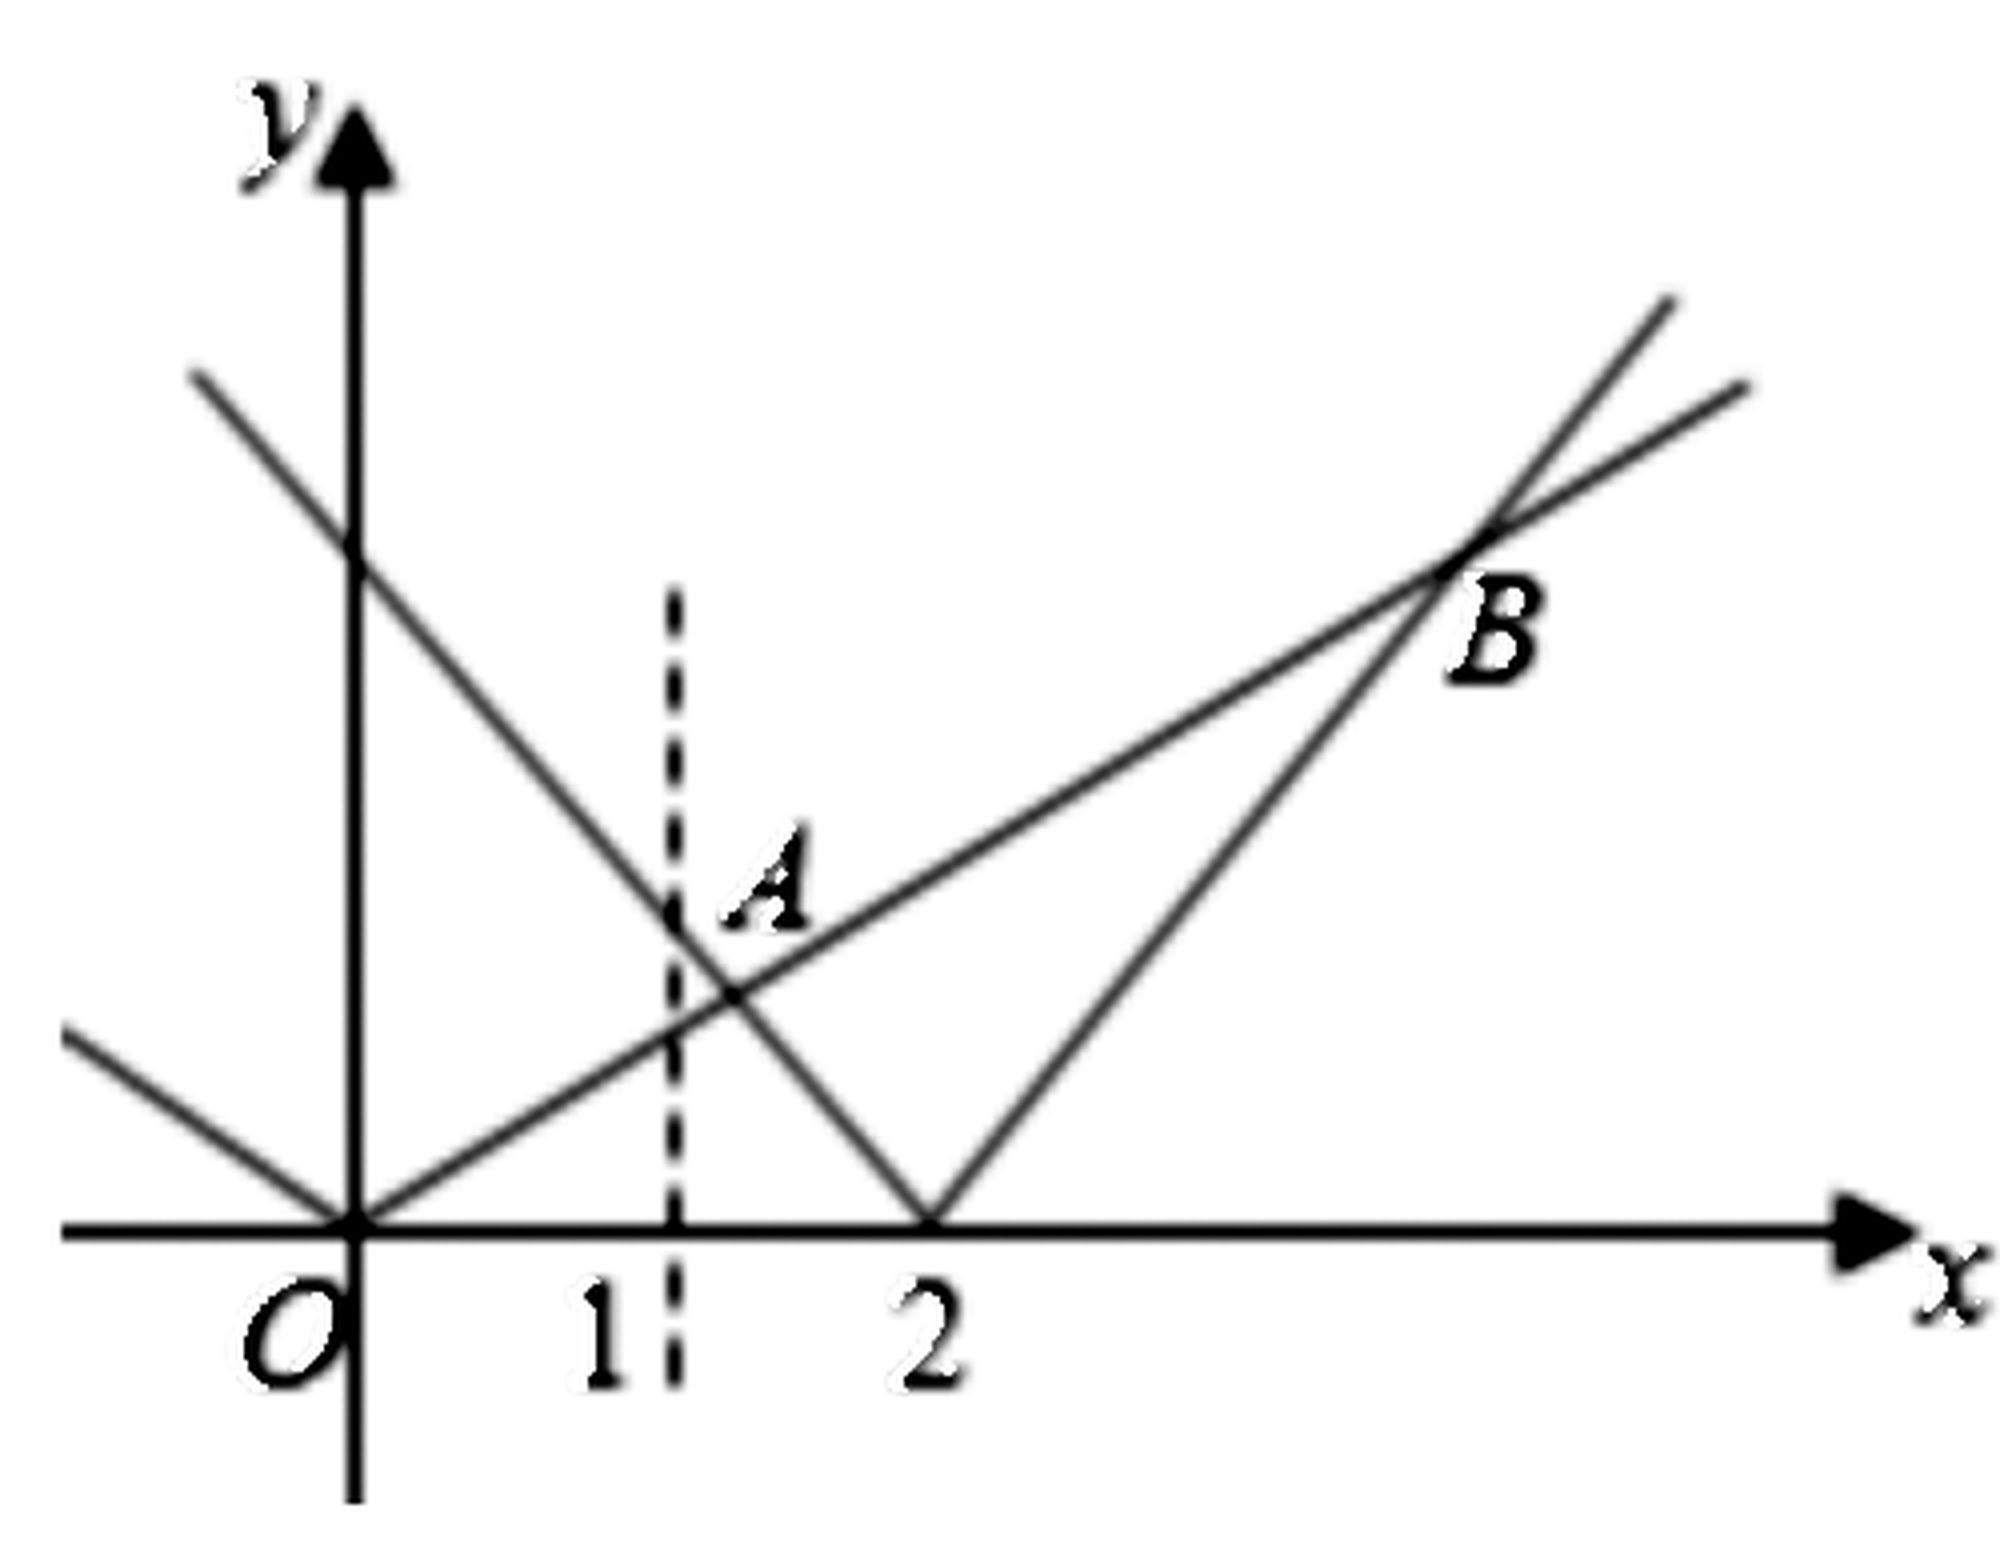
\includegraphics[width=0.40\textwidth]{figures/gao152_q15.png}
\end{center}
\step{由 $0<k<1$，得 $x_A>1$，}
\step{所以关于 $x$ 的不等式 $k\lvert x\rvert-\lvert x-2\rvert>0$ 恰好有 4 个整数解，是 2，3，4，5，}
\step{由 $\begin{cases}y=kx\\y=x-2\end{cases}\Rightarrow x_B=\dfrac2{1-k}\in(5,6]$，故 $\dfrac35<k\leqslant\dfrac23$；故选 $B$.}
\solend
\fi

% === Q16 === 咖啡优惠题；解析 12 行（跨 04 页上下半）；故选 C
\item 上海是全球咖啡店最多的城市. 若某品牌的某种在售咖啡产品价格为 30 元/杯，其原材料成本为 7 元/杯，营销成本为 5 元/杯，且该品牌门店提供如下 4 种优惠方式：(1) 首杯免单，每人限用一次；(2) 3.8 折优惠券，每人限用一次；(3) 买 2 杯送 2 杯，每人限用两次；(4) 买 5 杯送 5 杯，不限使用人数和使用次数. 每位消费者都可以在以上 4 种优惠方式中选择不多于 2 种使用. 现在某个公司有 5 位后勤工作人员去该品牌门店帮每位技术人员购买 1 杯咖啡，购买杯数与技术人员人数须保持一致；请问，这个公司的技术人员不少于\mbox{（\quad）}人时，无论 5 位后勤人员采用什么样的优惠方式购买咖啡，这笔订单该品牌门店都能保证盈利.

\keepwithprev
A. 20\qquad\qquad B. 25\qquad\qquad C. 30\qquad\qquad D. 35

\ifanswer
\solbegin
\step{按各优惠不叠加于同一杯理解，3.8 折券仅用于一杯，}
\step{买赠中的购买杯按原价付款.}
\step{设共购 $n$ 杯，免单、券购、原价购买的杯数分别为 $a,b,c$，其中 $0\leqslant a,b\leqslant5$，}
\step{其余为买赠咖啡，每杯成本为 12 元，}
\step{利润为 $P=15(n-a-b-c)+11.4b+30c-12n=3n-15a-3.6b+15c$，}
\step{若 $a,b$ 不同时为 5，则 $15a+3.6b\leqslant75+14.4=89.4$，}
\step{当 $n\geqslant30$ 时，$P\geqslant90-89.4=0.6>0$.}
\step{若 $a=b=5$，则每人均已使用免单和优惠券两种方式，其余均须原价购买，}
\step{$P=57+30(n-10)-12n=18n-243\geqslant297>0$.}
\step{当 $n=29$ 时，4 人各用方式 (1)(2) 购得 2 杯，}
\step{另 1 人用方式 (1) 及两次方式 (4) 购得 21 杯，}
\step{此时 $P=4\times11.4+2\times150-29\times12=-2.4<0$，因此最小人数为 30，故选 $C$.}% $2\times150$ 为两次方式（4）各买 5 杯的付款，照录（见 ⑤ 3）
\solend
\fi

\end{enumerate}

\bigsec{三、解答题}

\begin{enumerate}
\setcounter{enumi}{16}

% === Q17 === 解集含 \R／\varnothing；解析 4 行
\item 若 $a$、$b\in\R$，求关于 $x$ 的不等式 $ax\geqslant b$ 的解集.

\ifanswer
\solbegin
\step{当 $a>0$ 时，原不等式的解集为 $\left\{x\mid x\geqslant\dfrac ba\right\}$；}
\step{当 $a<0$ 时，原不等式的解集为 $\left\{x\mid x\leqslant\dfrac ba\right\}$；}
\step{当 $a=0$，$b\leqslant0$ 时，原不等式的解集为 $\R$；}
\step{当 $a=0$，$b>0$ 时，原不等式的解集为 $\varnothing$.}
\solend
\fi

% === Q18 === 子集 ⊆ 两处照录；cases 块；解析 9 行（跨 05 页上下半）
\item 已知 $\alpha:x<3m-1$ 或 $x>-m$，$\beta:x<2$ 或 $x\geqslant4$.

(1) 若 $\alpha$ 是 $\beta$ 的充分条件，求实数 $m$ 的取值范围；

(2) 若 $\alpha$ 是 $\beta$ 的必要条件，求实数 $m$ 的取值范围.

\ifanswer
\solbegin
\step{(1) 设 $A=\{x\mid x<3m-1\text{ 或 }x>-m\}$，$B=\{x\mid x<2\text{ 或 }x\geqslant4\}$，}
\step{因为 $\alpha$ 是 $\beta$ 的充分条件，所以 $A\subseteq B$，}
\step{当 $3m-1>-m$ 时，即 $m>\dfrac14$，此时 $A=\R$，不满足题意；}
\step{当 $3m-1\leqslant-m$ 时，即 $m\leqslant\dfrac14$，有 $\begin{cases}3m-1\leqslant2\\-m\geqslant4\end{cases}$，解得 $m\leqslant-4$；}
\step{综上，$m$ 的取值范围为 $(-\infty,-4]$.}
\step{(2) 因为 $\alpha$ 是 $\beta$ 的必要条件，所以 $B\subseteq A$，}
\step{当 $3m-1>-m$ 时，即 $m>\dfrac14$，此时 $A=\R$，$B\subseteq A$ 成立；}
\step{当 $3m-1\leqslant-m$ 时，即 $m\leqslant\dfrac14$，有 $\begin{cases}3m-1\geqslant2\\-m<4\end{cases}$，无解.}
\step{综上，$m$ 的取值范围为 $\left[\dfrac14,+\infty\right)$.}
\solend
\fi

% === Q19 === \varnothing 空集照录；解析 9 行
\item 设关于 $x$ 的不等式 $x^2+4x+k-1\geqslant0$ 的解集为 $A$.

(1) 若 $A=\R$，求实数 $k$ 的取值范围；

(2) 求证：不存在实数 $k$，使得 $A=\varnothing$.

\ifanswer
\solbegin
\step{(1) 配方得 $x^2+4x+k-1=(x+2)^2+k-5$，}
\step{若 $A=\R$，取 $x=-2$，得 $k-5\geqslant0$，即 $k\geqslant5$.}
\step{当 $k\geqslant5$ 时，对任意 $x\in\R$，都有 $(x+2)^2+k-5\geqslant0$，因此 $A=\R$.}
\step{所以 $k$ 的取值范围为 $[5,+\infty)$.}
\step{(2) 当 $k\geqslant5$ 时，由 (1) 得 $A=\R\ne\varnothing$.}
\step{当 $k<5$ 时，取 $x_0=-2+\sqrt{5-k}$，}
\step{则 $x_0^2+4x_0+k-1=(x_0+2)^2+k-5=(5-k)+k-5=0$，}
\step{所以 $x_0\in A$，即 $A\ne\varnothing$.}
\step{因此，不存在实数 $k$，使得 $A=\varnothing$.}
\solend
\fi

% === Q20 === |A\cap B|=1 印等号；等腰偏高粗 \Delta 照录；解析 12 行（跨 06→07 页）
\item 设 $m\in\R$. 集合 $A=\left\{x\mid\dfrac{x^2+x}{x+1}\geqslant\dfrac{2x+m}{x},x\in\R\right\}$，
$B=\left\{x\mid\dfrac{x^2+x}{x+1}\leqslant\dfrac{2x+m}{x},x\in\R\right\}$.

(1) 若 $m=8$，记集合 $M=A\cap(0,+\infty)$，求集合 $M$；

(2) 用 $\lvert T\rvert$ 代表集合 $T$ 的元素个数. 若 $\lvert A\cap B\rvert=1$，记 $m$ 的取值集合为 $C$，试比较 $\lvert C\rvert$ 与 2 的大小，并证明你的结论.

\ifanswer
\solbegin
\step{(1) 当 $m=8$，$x>0$ 时，$\dfrac{x^2+x}{x+1}\geqslant\dfrac{2x+8}{x}\Leftrightarrow x^2-2x-8\geqslant0$}
\step{$\Leftrightarrow(x-4)(x+2)\geqslant0\Leftrightarrow x\geqslant4$，所以 $M=[4,+\infty)$.}
\step{(2) 原分式有意义须 $x\ne-1,0$，因此 $x\in A\cap B\Leftrightarrow\begin{cases}x^2-2x-m=0\\x\ne-1,0\end{cases}$，}
\step{方程的判别式为 $\Delta=4(1+m)$.}
\step{当 $m<-1$ 时，方程无实根，$\lvert A\cap B\rvert=0$；}
\step{当 $m=-1$ 时，方程只有一个实根 1，$A\cap B=\{1\}$.}
\step{当 $m>-1$ 时，方程有两个不同实根.}
\step{其中，0 为根当且仅当 $m=0$，$-1$ 为根当且仅当 $m=3$.}
\step{$m=0$ 时，方程的根为 $0,2$，$A\cap B=\{2\}$；}
\step{$m=3$ 时，方程的根为 $-1,3$，$A\cap B=\{3\}$.}
\step{$m>-1$ 且 $m\ne0,3$ 时，两个实根均满足原分式的定义条件，$\lvert A\cap B\rvert=2$.}
\step{因此 $C=\{-1,0,3\}$，$\lvert C\rvert=3>2$.}
\solend
\fi

% === Q21 === "性质 p"新定义、\Q 归一、M\subseteq\R 照录；解析 19 行（跨 07→08 页）
\item 设集合 $M\subseteq\R$. 若 $M$ 中元素个数大于等于 2，且 $M$ 的任意不同元素 $a$、$b$ 均满足 $a^3-\dfrac14b\in M$，则称集合 $M$ 具有“性质 $p$”.

(1) 试判断集合 $\Q$、集合 $\left\{-\dfrac{\sqrt3}{2},0,\dfrac{\sqrt3}{2}\right\}$ 是否具有“性质 $p$”，并说明理由；

(2) 设 $m$ 为大于等于 2 的正整数. 若集合 $A=\{x_1,x_2,\cdots,x_m\}$，且具有“性质 $p$”，求证：$m=2$，并求集合 $A$ 中所有元素的乘积.

\ifanswer
\solbegin
\step{(1) $\Q$ 中至少有两个元素，且任意不同的 $a,b\in\Q$ 均满足 $a^3-\dfrac14b\in\Q$，}
\step{故 $\Q$ 具有“性质 $p$”.}
\step{对于另一集合，取 $a=0$，$b=\dfrac{\sqrt3}{2}$，则 $a^3-\dfrac14b=-\dfrac{\sqrt3}{8}$ 不属于该集合，}
\step{故其不具有“性质 $p$”.}
\step{(2) 将 $A$ 中元素按 $x_1<x_2<\cdots<x_m$ 排列.}
\step{若 $m\geqslant3$，由性质 $p$ 及幂函数 $y=x^3$ 的单调性，}
\step{有 $x_1^3-\dfrac14x_m<\cdots<x_1^3-\dfrac14x_2<x_m^3-\dfrac14x_2<x_m^3-\dfrac14x_1$，}
\step{上述 $m+1$ 个互不相同的数均属于 $A$，与 $A$ 只有 $m$ 个元素矛盾，}
\step{因此 $m=2$.}
\step{设 $A=\{a,b\}$，$a<b$.}
\step{因为 $a^3-\dfrac14b<b^3-\dfrac14a$，且两者均属于 $A$，}
\step{所以 $a^3-\dfrac14b=a$，$b^3-\dfrac14a=b$，}
\step{两式相减并除以 $a-b\ne0$，}
\step{以及两式相加，分别得 $a^2+ab+b^2=\dfrac34$，$(a+b)(a^2-ab+b^2)=\dfrac54(a+b)$，}
\step{代入 $a^2-ab+b^2=\dfrac34-2ab$，得 $(a+b)(4ab+1)=0$，}
\step{若 $a+b=0$，则 $-ab=a^2+ab+b^2=\dfrac34$，即 $ab=-\dfrac34$；}
\step{若 $a+b\ne0$，则 $ab=-\dfrac14$.}
\step{分别取 $A=\left\{-\dfrac{\sqrt3}{2},\dfrac{\sqrt3}{2}\right\}$，$A=\left\{\dfrac{1-\sqrt3}{2\sqrt2},\dfrac{1+\sqrt3}{2\sqrt2}\right\}$，}
\step{代入均有 $a^3-\dfrac14b=a$、$b^3-\dfrac14a=b$，故两种乘积均可取得.}
\solend
\fi

\end{enumerate}

\end{document}
"
% 紧凑版：xelatex "\def\iscompact{1}% 高一152_位育中学_期中.tex
%   —— 高一上数学"2026-2027 年位育中学高一上期中"（试卷版/答案版/紧凑版）
% 试卷版：xelatex 高一152_位育中学_期中.tex
% 答案版：xelatex "\def\isanswer{1}% 高一152_位育中学_期中.tex
%   —— 高一上数学"2026-2027 年位育中学高一上期中"（试卷版/答案版/紧凑版）
% 试卷版：xelatex 高一152_位育中学_期中.tex
% 答案版：xelatex "\def\isanswer{1}\input{高一152_位育中学_期中.tex}"
% 紧凑版：xelatex "\def\iscompact{1}\input{高一152_位育中学_期中.tex}"
%
% ① 原始材料：微信公众号"魔都数学加油站"文章，连载"27学年高一152"，原文标题
% "27学年高一152——2026-2027年上海市位育中学高一上期中"；
% 原文链接：https://mp.weixin.qq.com/s/v4_G6oTX2BuPz9L-KtLRfw 。
% 正文为 8 张 PNG 页（01/03/05/06/07/08 为 2560×3620，02/04 为 4762×6735，
% 同一篇各页分辨率混排，逐页按各自分辨率裁图核对，别按预览比例换算裁框）。
% 体例：讲评版——填空 3—12（10 题）、选择 13—16（4 题）、解答 17—21（5 题），
% 共 19 题，自第 3 题起编；题目、答案、解析均据原图转录；卷面粉红色水印
% "魔都数学加油站"及公众号页脚未录入。
% 全卷插图清单（逐页通读 8 页确认）：1 幅——第 15 题解析配图（两条折线
% $y=k\lvert x\rvert$ 与 $y=\lvert x-2\rvert$ 及坐标图，03 页右下，含 O、1、2、
% A、B 与虚线 $x=1$），解析写"的图象如下"，仅答案版出，裁
% figures/gao152_q15.png（去粉水印、去色、4× LANCZOS 放大）。
%
% 卷首标题：原卷印作"2026-2027 年位育中学高一上期中"，年份区间按全稿惯例排 en dash；
% 原卷卷面未印副标题，本稿按同期中卷知识模块口径补出"集合与常用逻辑用语、不等式、函数"。
%
% ② 与原卷的排版差异：
%   ① 原文从第 3 题起，本稿保留原题号；共 19 题三节，解答题 5 题到 21；
%   ② 混合体例：第 3、5 题只印【答案】、无【解析】，按 高一140 第 5 题／
%      高一145 第 3 题成例另提 \ans{}、不补造解析；第 13、14 题把答案"D"
%      直接印在题干括号内、题下无【解析】，按 高一84／148／149 成例括号留空、
%      另提 \ans{$D$}；其余 15 题印【解析】、用 \solbegin…\solend；
%      第 15、16 题答案在解析末句"故选 B／C"、括号留空、不另提 \ans{}；
%      答案版【答案】/【解析】标记数 = 19 = 全卷题数（4 个 \ans ＋ 15 个 \solbegin）；
%   ③ 原卷卷面未印副标题，本稿按知识模块口径补出；
%   ④ 原卷填空横线按全稿惯例排 \blankline[4.4em]；选择题括号排 \mbox{（\quad）}、
%      四道选择题的选项段前按惯例各加 \keepwithprev；解答题不留作答区、不加
%      \anspace（原卷为讲评版，109—113 起全稿不用 \anspace）；
%   ⑤ 数集黑板粗体：Q7"全集为 R"、Q9"$\lVert PQ\rVert$ 定义"无数集、
%      Q12"$t\in Z$"、Q13"$k\in Z$ 与 $=\R$"、Q17"$a,b\in R$"、Q19"$A=\R$"、
%      Q20"$m\in\R$"、Q21"$M\subseteq\R$ 与集合 $\Q$"原卷印正体粗体或黑板体
%      R/Q/Z，按全稿惯例归一 \R／\Q／\Z；绝对值排 \lvert…\rvert
%      （Q4、Q9、Q11、Q15），集合描述竖线排 \mid（Q7、Q13、Q20、Q21），
%      距离双竖线排 \lVert…\rVert（Q9 与题干、解析的 ||PQ||／||AB||）；
%      不等号按全稿惯例排 \leqslant／\geqslant；补集照原卷上划线排 \overline{A}
%      （Q7 题干＋解析）；空集 \varnothing（Q17、Q19）；
%      子集 Q18 两处、Q21 题干一处均印带下划线 ⊆、照录 \subseteq（见 ④），
%      本卷无单线 \subset 用例；
%   ⑥ 判别式 Δ/△ 两形混用逐处照录、不得统一：Q11 解析"判别式 △=k²−8k>0"
%      印扁等边细线三角、照录 \triangle，Q20 (2) 解析"判别式为 Δ=4(1+m)"
%      印等腰偏高粗三角、照录 \Delta（/tmp/gao152/z/zoom/q11_delta.png、
%      q20_delta.png 放大并与 151 卷同型并排比较）；
%   ⑦ 中文弯引号照录：Q11"长度"、Q21"性质 p"（题干、两问与解析多处）、
%      Q6 从">"、"<"、"≥"、"≤"中选符号、Q16"（1）…（4）"半角括号；
%      注释里一律 ASCII 引号；数学式内 CJK 用 \text{}（Q13 的"或／且"、
%      Q18 集合描述的"或"）；
%   ⑧ "图像／图象"：全卷仅 Q15 解析一处"的图象如下"，印"图象"（象，无亻）、
%      照录；其余各题无"图像"字样。子题标号 (1)(2)(3)(4) 半角括号照录；
%   ⑨ 半角逗号在数学组之间是全稿惯例、非笔误，逐处照录（Q6、Q10、Q16、
%      Q20、Q21 的 $a,b,c$ 之类）；行末西文句点 ASCII `.`；
%      行中全角逗号／顿号照录（Q11"（a,b）"、Q16"7 元/杯"、Q21"$\Q$、集合"）；
%   ⑩ 复杂式照录别简化：Q4 四组 cases 块（整体各占一个印刷行）、Q8
%      $\frac{x_0}{e^{x_0}}=\frac13$、Q10 $4a^2+b^2=4$、Q12 $b=\frac2a$、
%      Q16 利润式 $P=15(n-a-b-c)+11.4b+30c-12n$、Q18 cases 块、
%      Q20 分式 $\frac{x^2+x}{x+1}$、Q21 $a^3-\frac14b$ 与两组取值集合；
%      \left…\right 不得拆到不同 $…$ 组（Q4 cases 前的 \left\{ 一律改
%      \begin{cases}…\end{cases}、Q17 $\left\{x\mid x\ge\frac ba\right\}$、
%      Q20 $\left\{x\mid\cdots\right\}$、Q21 $\left\{-\frac{\sqrt3}2,\ldots\right\}$）；
%   ⑪ 一条 \step = 原卷解析的一个印刷行，cases 块整体算一个印刷行；别并折行、
%      别拆行。Q12 七行、Q16 十二行、Q18 九行、Q19 九行、Q20 十二行、
%      Q21 十九行均按印刷行逐条断，不丢行；
%   ⑫ 配图：Q15 解析配图（仅答案版出）放 \ifanswer 内 \solbegin…\solend 的
%      \step 之间（高一73 第 16 题／高一150 Q12 成例）；题干无配图，故无
%      \needvspace；
%   ⑬ 原卷解析内无红色"法一／法二"之类小标题，故本卷无 \stepm；红色水印
%      "魔都数学加油站"不录入；
%   ⑭ 跨页续印按题合并：见 ⑥；
%
% ③ 行数复核：一条 \step = 原卷解析的一个印刷行，cases 块作一个印刷行计。
%   逐题数（主会话逐页核对定稿）：Q3：0（只印【答案】、提 \ans{}）；Q4：2；
%   Q5：0（只印【答案】、提 \ans{}）；Q6：1；Q7：1；Q8：1；Q9：1；
%   Q10：4；Q11：5；Q12：7；Q13：0（答案印括号内、提 \ans{}）；
%   Q14：0（答案印括号内、提 \ans{}）；Q15：4；Q16：12；Q17：4；
%   Q18：9；Q19：9；Q20：12；Q21：19。
%   合计 91 条 \step（本卷无 \stepm），与原卷逐题印刷行相等。全卷 15 题设
%   \solbegin…\solend ＋ Q3／Q5／Q13／Q14 四处 \ans{}，答案版
%   【答案】/【解析】标记数 = 19 = 全卷题数。
%
% ④ 判别式／子集符号结论（逐处放大原图照录、不得统一，主会话像素级复核）：
%   判别式：Q11 解析"方程 $x^2-kx+2k=0$ 的判别式 $\triangle=k^2-8k>0$"
%      印扁等边细线三角、照录 \triangle；Q20 (2) 解析"方程的判别式为
%      $\Delta=4(1+m)$"印等腰偏高粗三角、照录 \Delta
%      （/tmp/gao152/z/zoom/q11_delta.png、q20_delta.png；与 高一142／151
%      的"Δ/△ 混用逐处照录"口径一致）。本卷无几何三角形符号。
%   子集：Q18 解析 (1)"$A\subseteq B$"、(2)"$B\subseteq A$"与 Q21 题干
%      "$M\subseteq\R$"共 3 处均印带下划线 ⊆、照录 \subseteq
%      （/tmp/gao152/z/zoom/q18_subset.png、q21_subset.png 放大确认）；
%      本卷无单线 ⊂ 用例。补集上划线 \overline{A}（Q7）、空集 \varnothing
%      （Q17 解析末行、Q19 题干 (2) 与解析）、数集 \R／\Q／\Z 归一见 ② ⑤。
%
% ⑤ 存疑照录（放大原图确认，照录未改、正文对应处另有 % 注）：
%   1. Q11 题干"已知关于 $x$ 的不等式 $x^2-kx+2k<0$ 有实数解，且解集区间
%      长度不超过 3 个单位"，解析据 $\lvert x_1-x_2\rvert\leqslant3$ 推；
%      判别式用扁三角 \triangle（见 ④），照录未改。
%   2. Q12 解析"$t=-1$ 时取 $b=\frac2a\in[-2,-1]$，$c=-1$，则 $ab+c=2-1=1$"
%      ——$b$ 径写 $\frac2a$（无负号），放大 03 页确认，照录未改。
%   3. Q16 解析"$P=4\times11.4+2\times150-29\times12=-2.4<0$"中的
%      $2\times150$ 为两次方式（4）各买 5 杯的付款，照录未改。
%   4. Q20 (2) 题干"若 $\lvert A\cap B\rvert=1$"印等号（非 $\leqslant1$），
%      放大 06 页 /tmp/gao152/z/zoom/q20_eq1.png 确认，照录未改。
%   5. Q21 题干"性质 p"用弯引号且 $p$ 为斜体小写，逐处照录未统一；
%      解析 (2) 末两组 $A$ 的取值集合照录未简化。
%   6. "图像／图象"仅 Q15 一处"图象"、Δ/△ 两形并用（Q11 \triangle、
%      Q20 \Delta）均逐处照录、未统一（见 ② ⑥ ⑧ 与 ④）。
%   全卷除此 6 类外未发现其它笔误／自相矛盾处；19 题中 15 题印【解析】、
%   Q3／Q5 只印【答案】、Q13／Q14 答案印题干括号内（见 ② ②）。
%
% ⑥ 跨页续印按题合并说明（逐页核实定稿）：Q3—Q5 题干＋【答案】／【解析】
%   在 01 页上半，Q6—Q8 题干＋解析在 01 页下半；Q9、Q10 题干＋解析、
%   Q11 题干＋解析、Q12 题干＋解析首行在 02 页；Q12 解析余 6 行续 03 页
%   上半，"二、选择题"标题与 Q13 题干＋选项在 03 页下半；Q13 选项 C／D、
%   Q14 题干＋四选项＋（无解析）、Q15 题干＋四选项＋解析前 3 行＋配图在
%   03 页下半，Q15 解析末行（由 cases 求 $x_B$）续 04 页顶；Q16 题干＋四选项
%   ＋解析前 5 行在 04 页上半，解析余 7 行在 04 页下半；"三、解答题"标题与
%   Q17 题干＋解析首行在 04 页末，Q17 解析余 3 行、Q18 题干＋两问＋解析首
%   4 行在 05 页上半，Q18 解析余 5 行在 05 页下半；Q19 题干＋两问＋解析
%   (1) 4 行在 05—06 页（(2) 题干续 06 页顶），解析 (2) 5 行在 06 页上半；
%   Q20 题干＋两问＋解析 (1) 2 行＋(2) 首行在 06 页下半；Q20 (2) 解析余
%   9 行、Q21 题干＋两问＋解析 (1) 4 行在 07 页；Q21 (2) 解析 19 行中前
%   6 行在 07—08 页上半、末 13 行续 08 页下半，末行"故两种乘积均可取得"
%   为全卷收尾（08 页下半仅水印、无其它正文）。
%   本稿按题连排，不丢行、不并折行；全卷末题为第 21 题，无附加题节。
%
\documentclass[a4paper,11pt]{article}
\usepackage{common}

\begin{document}

\examtitlest[3]{2026--2027 年位育中学高一上期中}{集合与常用逻辑用语、不等式、函数}

\bigsec{一、填空题}

\begin{enumerate}
\setcounter{enumi}{2}

% === Q3 === 原卷只印【答案】、无【解析】，另提 \ans{}，不补造解析
\item 设 $x>0$. 若 $\ln x=-1$，则 $x=$\blankline[4.4em].

\ifanswer
\ans{$\dfrac1{\mathrm{e}}$}
\fi

% === Q4 === 四组 cases 块同一印刷行；解析 2 行
\item 不等式 $\lvert 1-2x\rvert>x$ 的解集为\blankline[4.4em].

\ifanswer
\solbegin
\step{不等式 $\lvert 1-2x\rvert>x$ 即为 $\begin{cases}1-2x\geqslant0\\1-2x>x\end{cases}$ 或 $\begin{cases}1-2x<0\\2x-1>x\end{cases}$，即 $\begin{cases}x\leqslant\frac12\\x<\frac13\end{cases}$ 或 $\begin{cases}x>\frac12\\x>1\end{cases}$，}
\step{则有 $x<\dfrac13$ 或 $x>1$，则解集为 $\left(-\infty,\dfrac13\right)\cup(1,+\infty)$.}
\solend
\fi

% === Q5 === 原卷只印【答案】、无【解析】；\frac1x\ge1 印单线 ≥，按全稿惯例 \geqslant
\item 不等式 $\dfrac1x\geqslant1$ 的解集为\blankline[4.4em].

\ifanswer
\ans{$(0,1]$}
\fi

% === Q6 === 从四个符号中选一个，中文弯引号照录；解析 1 行
\item 设 $a$、$b>0$，则 $a^2+b^2$\blankline[4.4em]$2(2a-b)-5$（从“$>$”、“$<$”、“$\geqslant$”、“$\leqslant$”中选择一个符号填写）.

\ifanswer
\solbegin
\step{$a^2+b^2-[2(2a-b)-5]=(a-2)^2+(b+1)^2>0$，故 $a^2+b^2>2(2a-b)-5$.}
\solend
\fi

% === Q7 === 补集上划线 \overline{A}；集合描述竖线 \mid；解析 1 行
\item 已知全集为 $\R$，集合 $A=\{x\mid y=\sqrt{x-2}\}$，集合 $B=\{y\mid y=\sqrt{x-2}\}$，则 $\overline{A}\cap B=$\blankline[4.4em].

\ifanswer
\solbegin
\step{$A=[2,+\infty)$，$B=[0,+\infty)$，所以 $\overline{A}\cap B=[0,2)$.}
\solend
\fi

% === Q8 === \frac{x_0}{e^{x_0}}=\frac13 照录；解析 1 行
\item 设正数 $x_0$ 满足等式 $\dfrac{x_0}{e^{x_0}}=\dfrac13$，则 $x_0-\ln x_0=$\blankline[4.4em].

\ifanswer
\solbegin
\step{等式两边取自然对数，得 $\ln x_0-x_0=-\ln3$，即 $x_0-\ln x_0=\ln3$.}
\solend
\fi

% === Q9 === 距离双竖线 \lVert…\rVert；解析 1 行
\item 在平面直角坐标系 $xOy$ 中，设点 $P(x_1,y_1)$，$Q(x_2,y_2)$，定义：$\lVert PQ\rVert=\lvert x_1-x_2\rvert+\lvert y_1-y_2\rvert$. 若点 $A(1,0)$，点 $B$ 为直线 $y=x+2$ 上的动点，则 $\lVert AB\rVert$ 的最小值为\blankline[4.4em].

\ifanswer
\solbegin
\step{$\lVert AB\rVert=\lvert x-1\rvert+\lvert y\rvert=\lvert x-1\rvert+\lvert x+2\rvert\geqslant3$，最小值为 3.}
\solend
\fi

% === Q10 === 解析 4 行
\item 已知 $a$、$b$ 均为正数，且 $a^2+\dfrac14b^2=1$，则 $a\sqrt{1+b^2}$ 的最大值为\blankline[4.4em].

\ifanswer
\solbegin
\step{因为 $a$、$b$ 均为正数，且 $a^2+\dfrac14b^2=1$，所以 $4a^2+b^2=4$，}
\step{所以 $a\sqrt{1+b^2}=\dfrac12\cdot2a\cdot\sqrt{1+b^2}\leqslant\dfrac12\cdot\dfrac{4a^2+1+b^2}{2}=\dfrac54$，}
\step{当且仅当 $4a^2=b^2+1$ 即 $a=\dfrac{\sqrt{10}}4$，$b=\dfrac{\sqrt6}2$ 时取等号，}
\step{故 $a\sqrt{1+b^2}$ 的最大值为 $\dfrac54$.}
\solend
\fi

% === Q11 === 扁等边细线判别式 \triangle 照录（见 ④）；"长度"弯引号；解析 5 行
\item 一般地，把 $b-a$ 称为区间 $(a,b)$ 的“长度”. 已知关于 $x$ 的不等式 $x^2-kx+2k<0$ 有实数解，且解集区间长度不超过 3 个单位，则实数 $k$ 的取值范围是\blankline[4.4em].

\ifanswer
\solbegin
\step{因为不等式 $x^2-kx+2k<0$ 有解，}
\step{所以方程 $x^2-kx+2k=0$ 的判别式 $\triangle=k^2-8k>0$，解得 $k>8$ 或 $k<0$，}
\step{由 $x_1+x_2=k$，$x_1x_2=2k$，得 $(x_1-x_2)^2=(x_1+x_2)^2-4x_1x_2=k^2-8k$，}
\step{由 $\lvert x_1-x_2\rvert\leqslant3$，得 $(x_1-x_2)^2\leqslant9$，即 $k^2-8k\leqslant9$，解得 $-1\leqslant k\leqslant9$，}
\step{所以 $-1\leqslant k<0$ 或 $8<k\leqslant9$，即实数 $k$ 的取值范围是 $[-1,0)\cup(8,9]$.}
\solend
\fi

% === Q12 === $b=\frac2a$ 无负号、$c=-1$ 照录（见 ⑤ 2）；解析 7 行（跨 02→03 页）
\item 设 $t\in\Z$，且对任意 $a\in[-2,t]$，总存在 $b,c\in[-2,t]$，使得 $ab+c=1$，则 $t$ 的所有取值为\blankline[4.4em].

\ifanswer
\solbegin
\step{$[-2,t]$ 是区间，要求 $t>-2$，故 $t\geqslant-1$.}
\step{当 $t\geqslant1$ 时，对任意 $a\in[-2,t]$，}
\step{取 $b=0$，$c=1$，两者都属于 $[-2,t]$，且 $ab+c=1$.}
\step{当 $t=0$ 时，取 $a=0$，则 $c=1\notin[-2,0]$，不成立.}
\step{当 $t=-1$ 时，对任意 $a\in[-2,-1]$，取 $b=\dfrac2a\in[-2,-1]$，$c=-1$，}% 原卷径写 $b=\frac2a$（无负号），放大 03 页确认，照录未改（见 ⑤ 2）
\step{则 $ab+c=2-1=1$.}
\step{所以 $t=-1$ 或 $t\geqslant1$（$t\in\Z$）.}
\solend
\fi

\end{enumerate}

\bigsec{二、选择题}

\begin{enumerate}
\setcounter{enumi}{12}

% === Q13 === 答案 D 印在题干括号内、无【解析】，按 高一84／148／149 成例括号留空、另提 \ans{}
\item 下列说法错误的是\mbox{（\quad）}

\keepwithprev
A. 奇数集可以表示为 $\{x\mid x=2k+1,k\in\Z\}$

B. 奇数集可以表示为 $\{x\mid x=2k-1,k\in\Z\}$

C. $\{x\mid x\ne2\text{ 或 }x\ne-2\}=\R$

D. $\{x\mid x\ne2\text{ 且 }x\ne-2\}=\R$

\ifanswer
\ans{$D$}
\fi

% === Q14 === 答案 D 印在题干括号内、无【解析】；选项两行两列
\item 设 $a$、$b$、$c>0$，且 $a\ne1$，则以下代数式中，不恒成立的是\mbox{（\quad）}

\keepwithprev
A. $\log_a 1=0$\qquad\qquad B. $a^{\log_a b}=b$

C. $\log_a b+\log_a c=\log_a(bc)$\qquad\qquad D. $\log_a b=\dfrac1{\log_b a}$

\ifanswer
\ans{$D$}
\fi

% === Q15 === "图象"（象，无亻）照录；解析配图仅答案版出；答案在解析末句故选 B
\item 若关于 $x$ 的不等式 $k\lvert x\rvert>\lvert x-2\rvert$ 恰好有 4 个整数解，则实数 $k$ 的取值范围是\mbox{（\quad）}

\keepwithprev
A. $\left(\dfrac35,\dfrac23\right)$\qquad B. $\left(\dfrac35,\dfrac23\right]$\qquad C. $\left(\dfrac35,1\right)$\qquad D. $\left(\dfrac35,1\right]$

\ifanswer
\solbegin
\step{由题意得 $0<k<1$，函数 $y=k\lvert x\rvert$ 与 $y=\lvert x-2\rvert$ 的图象如下，}
\begin{center}
% 两条折线坐标图取 03 页右下，去粉色水印、去色、4× LANCZOS 放大；仅答案版出
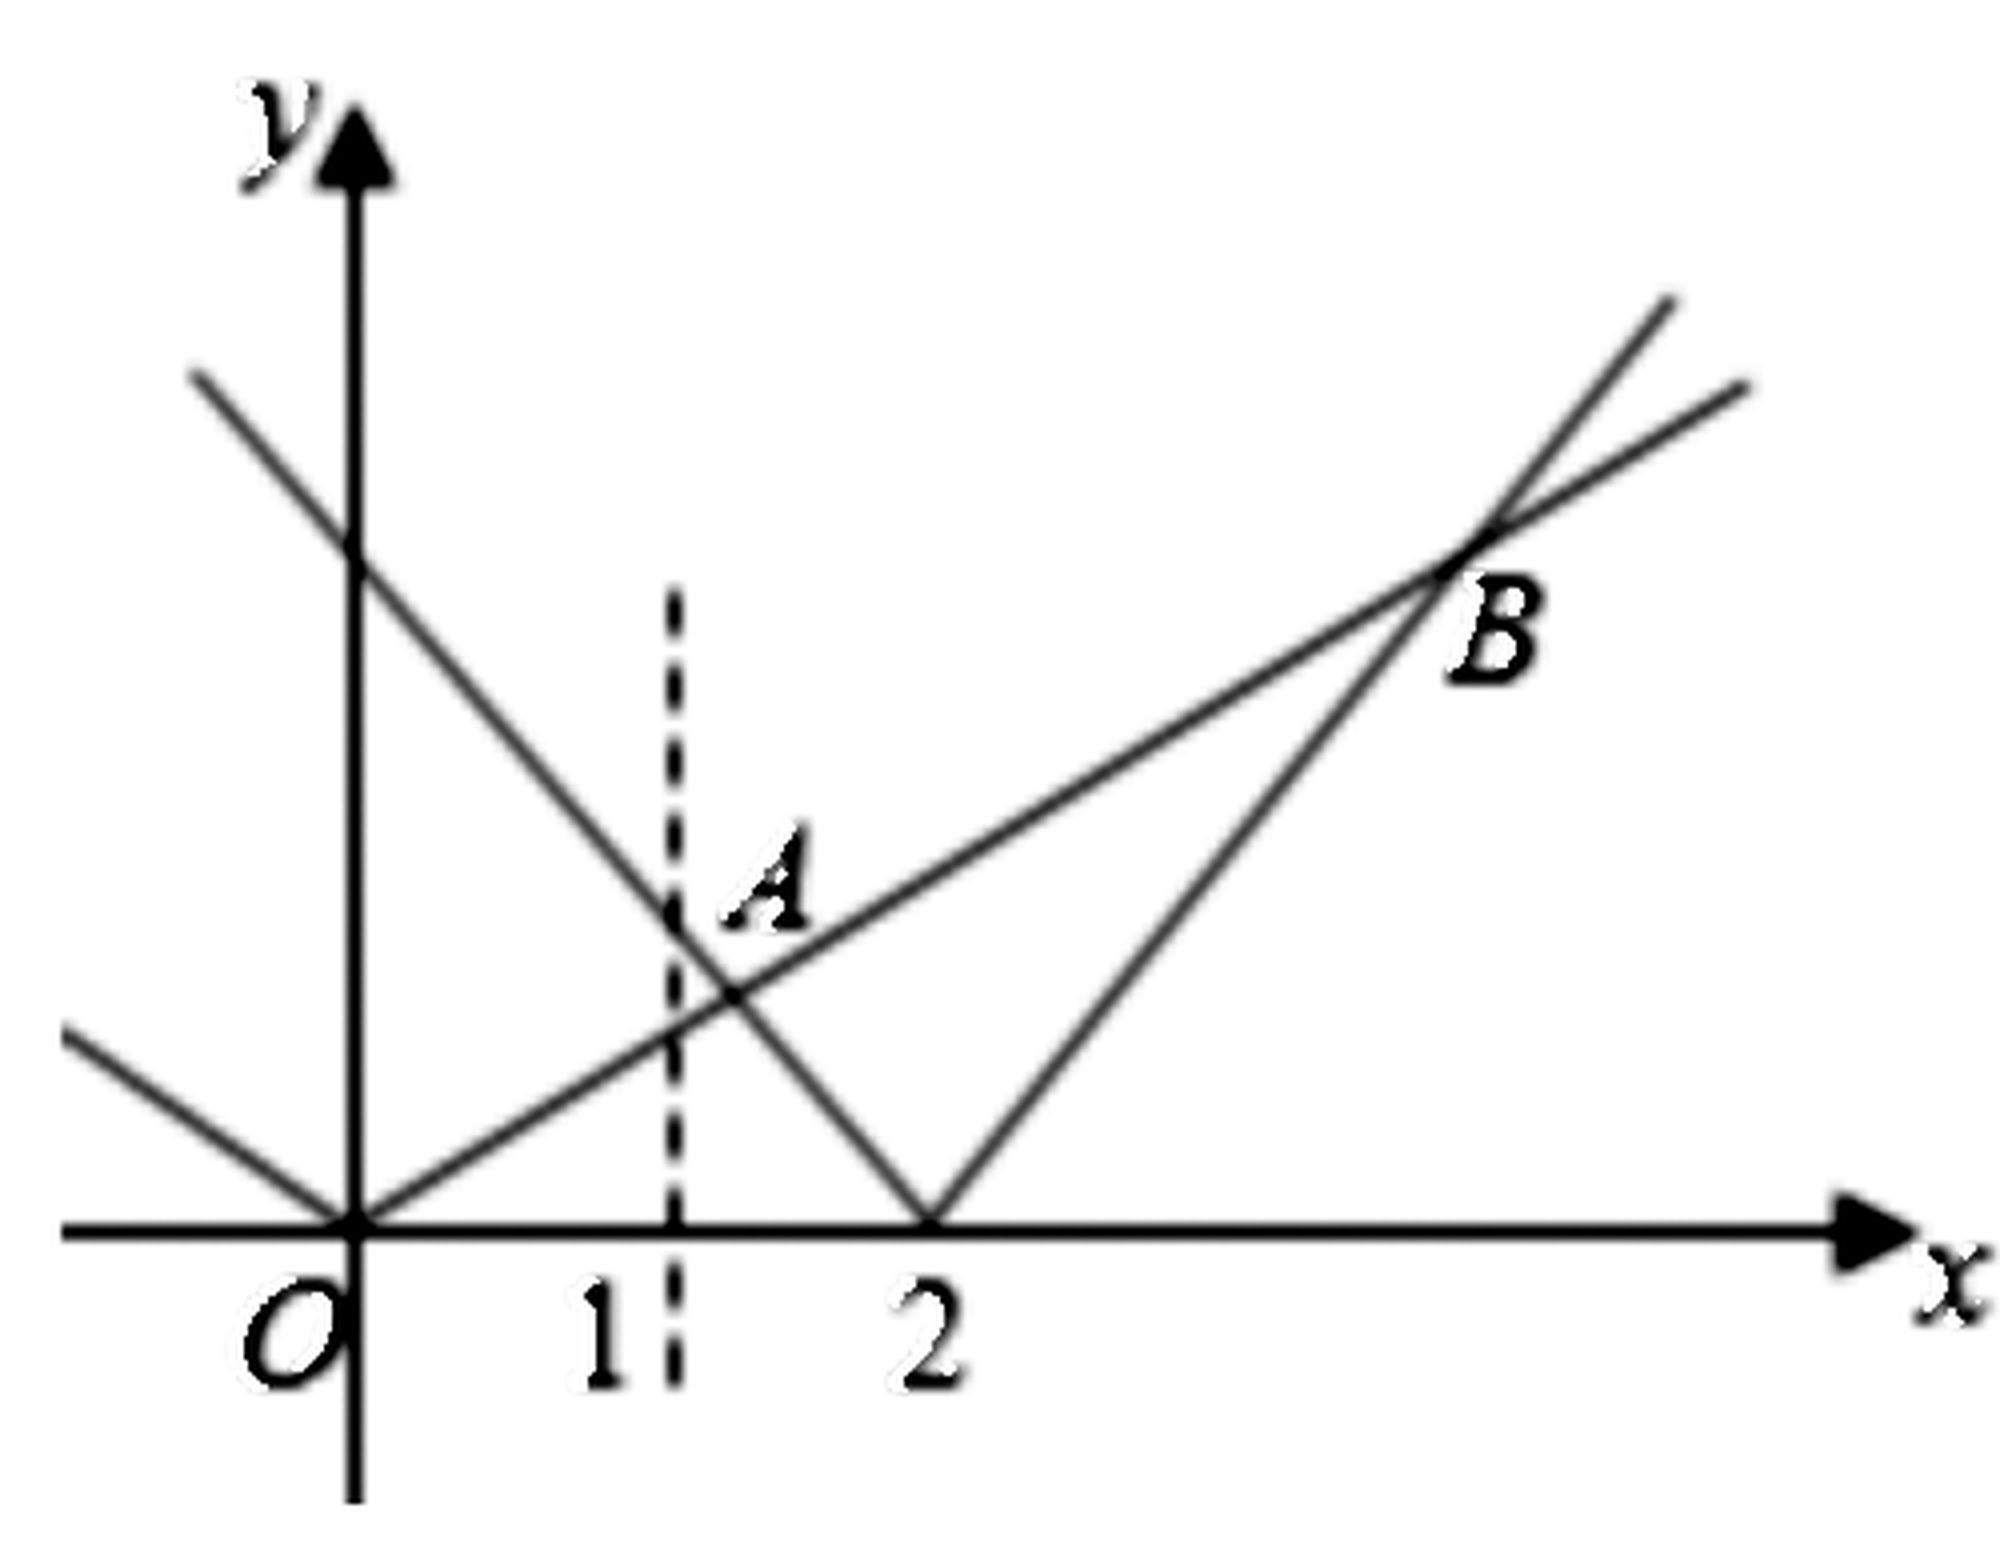
\includegraphics[width=0.40\textwidth]{figures/gao152_q15.png}
\end{center}
\step{由 $0<k<1$，得 $x_A>1$，}
\step{所以关于 $x$ 的不等式 $k\lvert x\rvert-\lvert x-2\rvert>0$ 恰好有 4 个整数解，是 2，3，4，5，}
\step{由 $\begin{cases}y=kx\\y=x-2\end{cases}\Rightarrow x_B=\dfrac2{1-k}\in(5,6]$，故 $\dfrac35<k\leqslant\dfrac23$；故选 $B$.}
\solend
\fi

% === Q16 === 咖啡优惠题；解析 12 行（跨 04 页上下半）；故选 C
\item 上海是全球咖啡店最多的城市. 若某品牌的某种在售咖啡产品价格为 30 元/杯，其原材料成本为 7 元/杯，营销成本为 5 元/杯，且该品牌门店提供如下 4 种优惠方式：(1) 首杯免单，每人限用一次；(2) 3.8 折优惠券，每人限用一次；(3) 买 2 杯送 2 杯，每人限用两次；(4) 买 5 杯送 5 杯，不限使用人数和使用次数. 每位消费者都可以在以上 4 种优惠方式中选择不多于 2 种使用. 现在某个公司有 5 位后勤工作人员去该品牌门店帮每位技术人员购买 1 杯咖啡，购买杯数与技术人员人数须保持一致；请问，这个公司的技术人员不少于\mbox{（\quad）}人时，无论 5 位后勤人员采用什么样的优惠方式购买咖啡，这笔订单该品牌门店都能保证盈利.

\keepwithprev
A. 20\qquad\qquad B. 25\qquad\qquad C. 30\qquad\qquad D. 35

\ifanswer
\solbegin
\step{按各优惠不叠加于同一杯理解，3.8 折券仅用于一杯，}
\step{买赠中的购买杯按原价付款.}
\step{设共购 $n$ 杯，免单、券购、原价购买的杯数分别为 $a,b,c$，其中 $0\leqslant a,b\leqslant5$，}
\step{其余为买赠咖啡，每杯成本为 12 元，}
\step{利润为 $P=15(n-a-b-c)+11.4b+30c-12n=3n-15a-3.6b+15c$，}
\step{若 $a,b$ 不同时为 5，则 $15a+3.6b\leqslant75+14.4=89.4$，}
\step{当 $n\geqslant30$ 时，$P\geqslant90-89.4=0.6>0$.}
\step{若 $a=b=5$，则每人均已使用免单和优惠券两种方式，其余均须原价购买，}
\step{$P=57+30(n-10)-12n=18n-243\geqslant297>0$.}
\step{当 $n=29$ 时，4 人各用方式 (1)(2) 购得 2 杯，}
\step{另 1 人用方式 (1) 及两次方式 (4) 购得 21 杯，}
\step{此时 $P=4\times11.4+2\times150-29\times12=-2.4<0$，因此最小人数为 30，故选 $C$.}% $2\times150$ 为两次方式（4）各买 5 杯的付款，照录（见 ⑤ 3）
\solend
\fi

\end{enumerate}

\bigsec{三、解答题}

\begin{enumerate}
\setcounter{enumi}{16}

% === Q17 === 解集含 \R／\varnothing；解析 4 行
\item 若 $a$、$b\in\R$，求关于 $x$ 的不等式 $ax\geqslant b$ 的解集.

\ifanswer
\solbegin
\step{当 $a>0$ 时，原不等式的解集为 $\left\{x\mid x\geqslant\dfrac ba\right\}$；}
\step{当 $a<0$ 时，原不等式的解集为 $\left\{x\mid x\leqslant\dfrac ba\right\}$；}
\step{当 $a=0$，$b\leqslant0$ 时，原不等式的解集为 $\R$；}
\step{当 $a=0$，$b>0$ 时，原不等式的解集为 $\varnothing$.}
\solend
\fi

% === Q18 === 子集 ⊆ 两处照录；cases 块；解析 9 行（跨 05 页上下半）
\item 已知 $\alpha:x<3m-1$ 或 $x>-m$，$\beta:x<2$ 或 $x\geqslant4$.

(1) 若 $\alpha$ 是 $\beta$ 的充分条件，求实数 $m$ 的取值范围；

(2) 若 $\alpha$ 是 $\beta$ 的必要条件，求实数 $m$ 的取值范围.

\ifanswer
\solbegin
\step{(1) 设 $A=\{x\mid x<3m-1\text{ 或 }x>-m\}$，$B=\{x\mid x<2\text{ 或 }x\geqslant4\}$，}
\step{因为 $\alpha$ 是 $\beta$ 的充分条件，所以 $A\subseteq B$，}
\step{当 $3m-1>-m$ 时，即 $m>\dfrac14$，此时 $A=\R$，不满足题意；}
\step{当 $3m-1\leqslant-m$ 时，即 $m\leqslant\dfrac14$，有 $\begin{cases}3m-1\leqslant2\\-m\geqslant4\end{cases}$，解得 $m\leqslant-4$；}
\step{综上，$m$ 的取值范围为 $(-\infty,-4]$.}
\step{(2) 因为 $\alpha$ 是 $\beta$ 的必要条件，所以 $B\subseteq A$，}
\step{当 $3m-1>-m$ 时，即 $m>\dfrac14$，此时 $A=\R$，$B\subseteq A$ 成立；}
\step{当 $3m-1\leqslant-m$ 时，即 $m\leqslant\dfrac14$，有 $\begin{cases}3m-1\geqslant2\\-m<4\end{cases}$，无解.}
\step{综上，$m$ 的取值范围为 $\left[\dfrac14,+\infty\right)$.}
\solend
\fi

% === Q19 === \varnothing 空集照录；解析 9 行
\item 设关于 $x$ 的不等式 $x^2+4x+k-1\geqslant0$ 的解集为 $A$.

(1) 若 $A=\R$，求实数 $k$ 的取值范围；

(2) 求证：不存在实数 $k$，使得 $A=\varnothing$.

\ifanswer
\solbegin
\step{(1) 配方得 $x^2+4x+k-1=(x+2)^2+k-5$，}
\step{若 $A=\R$，取 $x=-2$，得 $k-5\geqslant0$，即 $k\geqslant5$.}
\step{当 $k\geqslant5$ 时，对任意 $x\in\R$，都有 $(x+2)^2+k-5\geqslant0$，因此 $A=\R$.}
\step{所以 $k$ 的取值范围为 $[5,+\infty)$.}
\step{(2) 当 $k\geqslant5$ 时，由 (1) 得 $A=\R\ne\varnothing$.}
\step{当 $k<5$ 时，取 $x_0=-2+\sqrt{5-k}$，}
\step{则 $x_0^2+4x_0+k-1=(x_0+2)^2+k-5=(5-k)+k-5=0$，}
\step{所以 $x_0\in A$，即 $A\ne\varnothing$.}
\step{因此，不存在实数 $k$，使得 $A=\varnothing$.}
\solend
\fi

% === Q20 === |A\cap B|=1 印等号；等腰偏高粗 \Delta 照录；解析 12 行（跨 06→07 页）
\item 设 $m\in\R$. 集合 $A=\left\{x\mid\dfrac{x^2+x}{x+1}\geqslant\dfrac{2x+m}{x},x\in\R\right\}$，
$B=\left\{x\mid\dfrac{x^2+x}{x+1}\leqslant\dfrac{2x+m}{x},x\in\R\right\}$.

(1) 若 $m=8$，记集合 $M=A\cap(0,+\infty)$，求集合 $M$；

(2) 用 $\lvert T\rvert$ 代表集合 $T$ 的元素个数. 若 $\lvert A\cap B\rvert=1$，记 $m$ 的取值集合为 $C$，试比较 $\lvert C\rvert$ 与 2 的大小，并证明你的结论.

\ifanswer
\solbegin
\step{(1) 当 $m=8$，$x>0$ 时，$\dfrac{x^2+x}{x+1}\geqslant\dfrac{2x+8}{x}\Leftrightarrow x^2-2x-8\geqslant0$}
\step{$\Leftrightarrow(x-4)(x+2)\geqslant0\Leftrightarrow x\geqslant4$，所以 $M=[4,+\infty)$.}
\step{(2) 原分式有意义须 $x\ne-1,0$，因此 $x\in A\cap B\Leftrightarrow\begin{cases}x^2-2x-m=0\\x\ne-1,0\end{cases}$，}
\step{方程的判别式为 $\Delta=4(1+m)$.}
\step{当 $m<-1$ 时，方程无实根，$\lvert A\cap B\rvert=0$；}
\step{当 $m=-1$ 时，方程只有一个实根 1，$A\cap B=\{1\}$.}
\step{当 $m>-1$ 时，方程有两个不同实根.}
\step{其中，0 为根当且仅当 $m=0$，$-1$ 为根当且仅当 $m=3$.}
\step{$m=0$ 时，方程的根为 $0,2$，$A\cap B=\{2\}$；}
\step{$m=3$ 时，方程的根为 $-1,3$，$A\cap B=\{3\}$.}
\step{$m>-1$ 且 $m\ne0,3$ 时，两个实根均满足原分式的定义条件，$\lvert A\cap B\rvert=2$.}
\step{因此 $C=\{-1,0,3\}$，$\lvert C\rvert=3>2$.}
\solend
\fi

% === Q21 === "性质 p"新定义、\Q 归一、M\subseteq\R 照录；解析 19 行（跨 07→08 页）
\item 设集合 $M\subseteq\R$. 若 $M$ 中元素个数大于等于 2，且 $M$ 的任意不同元素 $a$、$b$ 均满足 $a^3-\dfrac14b\in M$，则称集合 $M$ 具有“性质 $p$”.

(1) 试判断集合 $\Q$、集合 $\left\{-\dfrac{\sqrt3}{2},0,\dfrac{\sqrt3}{2}\right\}$ 是否具有“性质 $p$”，并说明理由；

(2) 设 $m$ 为大于等于 2 的正整数. 若集合 $A=\{x_1,x_2,\cdots,x_m\}$，且具有“性质 $p$”，求证：$m=2$，并求集合 $A$ 中所有元素的乘积.

\ifanswer
\solbegin
\step{(1) $\Q$ 中至少有两个元素，且任意不同的 $a,b\in\Q$ 均满足 $a^3-\dfrac14b\in\Q$，}
\step{故 $\Q$ 具有“性质 $p$”.}
\step{对于另一集合，取 $a=0$，$b=\dfrac{\sqrt3}{2}$，则 $a^3-\dfrac14b=-\dfrac{\sqrt3}{8}$ 不属于该集合，}
\step{故其不具有“性质 $p$”.}
\step{(2) 将 $A$ 中元素按 $x_1<x_2<\cdots<x_m$ 排列.}
\step{若 $m\geqslant3$，由性质 $p$ 及幂函数 $y=x^3$ 的单调性，}
\step{有 $x_1^3-\dfrac14x_m<\cdots<x_1^3-\dfrac14x_2<x_m^3-\dfrac14x_2<x_m^3-\dfrac14x_1$，}
\step{上述 $m+1$ 个互不相同的数均属于 $A$，与 $A$ 只有 $m$ 个元素矛盾，}
\step{因此 $m=2$.}
\step{设 $A=\{a,b\}$，$a<b$.}
\step{因为 $a^3-\dfrac14b<b^3-\dfrac14a$，且两者均属于 $A$，}
\step{所以 $a^3-\dfrac14b=a$，$b^3-\dfrac14a=b$，}
\step{两式相减并除以 $a-b\ne0$，}
\step{以及两式相加，分别得 $a^2+ab+b^2=\dfrac34$，$(a+b)(a^2-ab+b^2)=\dfrac54(a+b)$，}
\step{代入 $a^2-ab+b^2=\dfrac34-2ab$，得 $(a+b)(4ab+1)=0$，}
\step{若 $a+b=0$，则 $-ab=a^2+ab+b^2=\dfrac34$，即 $ab=-\dfrac34$；}
\step{若 $a+b\ne0$，则 $ab=-\dfrac14$.}
\step{分别取 $A=\left\{-\dfrac{\sqrt3}{2},\dfrac{\sqrt3}{2}\right\}$，$A=\left\{\dfrac{1-\sqrt3}{2\sqrt2},\dfrac{1+\sqrt3}{2\sqrt2}\right\}$，}
\step{代入均有 $a^3-\dfrac14b=a$、$b^3-\dfrac14a=b$，故两种乘积均可取得.}
\solend
\fi

\end{enumerate}

\end{document}
"
% 紧凑版：xelatex "\def\iscompact{1}% 高一152_位育中学_期中.tex
%   —— 高一上数学"2026-2027 年位育中学高一上期中"（试卷版/答案版/紧凑版）
% 试卷版：xelatex 高一152_位育中学_期中.tex
% 答案版：xelatex "\def\isanswer{1}\input{高一152_位育中学_期中.tex}"
% 紧凑版：xelatex "\def\iscompact{1}\input{高一152_位育中学_期中.tex}"
%
% ① 原始材料：微信公众号"魔都数学加油站"文章，连载"27学年高一152"，原文标题
% "27学年高一152——2026-2027年上海市位育中学高一上期中"；
% 原文链接：https://mp.weixin.qq.com/s/v4_G6oTX2BuPz9L-KtLRfw 。
% 正文为 8 张 PNG 页（01/03/05/06/07/08 为 2560×3620，02/04 为 4762×6735，
% 同一篇各页分辨率混排，逐页按各自分辨率裁图核对，别按预览比例换算裁框）。
% 体例：讲评版——填空 3—12（10 题）、选择 13—16（4 题）、解答 17—21（5 题），
% 共 19 题，自第 3 题起编；题目、答案、解析均据原图转录；卷面粉红色水印
% "魔都数学加油站"及公众号页脚未录入。
% 全卷插图清单（逐页通读 8 页确认）：1 幅——第 15 题解析配图（两条折线
% $y=k\lvert x\rvert$ 与 $y=\lvert x-2\rvert$ 及坐标图，03 页右下，含 O、1、2、
% A、B 与虚线 $x=1$），解析写"的图象如下"，仅答案版出，裁
% figures/gao152_q15.png（去粉水印、去色、4× LANCZOS 放大）。
%
% 卷首标题：原卷印作"2026-2027 年位育中学高一上期中"，年份区间按全稿惯例排 en dash；
% 原卷卷面未印副标题，本稿按同期中卷知识模块口径补出"集合与常用逻辑用语、不等式、函数"。
%
% ② 与原卷的排版差异：
%   ① 原文从第 3 题起，本稿保留原题号；共 19 题三节，解答题 5 题到 21；
%   ② 混合体例：第 3、5 题只印【答案】、无【解析】，按 高一140 第 5 题／
%      高一145 第 3 题成例另提 \ans{}、不补造解析；第 13、14 题把答案"D"
%      直接印在题干括号内、题下无【解析】，按 高一84／148／149 成例括号留空、
%      另提 \ans{$D$}；其余 15 题印【解析】、用 \solbegin…\solend；
%      第 15、16 题答案在解析末句"故选 B／C"、括号留空、不另提 \ans{}；
%      答案版【答案】/【解析】标记数 = 19 = 全卷题数（4 个 \ans ＋ 15 个 \solbegin）；
%   ③ 原卷卷面未印副标题，本稿按知识模块口径补出；
%   ④ 原卷填空横线按全稿惯例排 \blankline[4.4em]；选择题括号排 \mbox{（\quad）}、
%      四道选择题的选项段前按惯例各加 \keepwithprev；解答题不留作答区、不加
%      \anspace（原卷为讲评版，109—113 起全稿不用 \anspace）；
%   ⑤ 数集黑板粗体：Q7"全集为 R"、Q9"$\lVert PQ\rVert$ 定义"无数集、
%      Q12"$t\in Z$"、Q13"$k\in Z$ 与 $=\R$"、Q17"$a,b\in R$"、Q19"$A=\R$"、
%      Q20"$m\in\R$"、Q21"$M\subseteq\R$ 与集合 $\Q$"原卷印正体粗体或黑板体
%      R/Q/Z，按全稿惯例归一 \R／\Q／\Z；绝对值排 \lvert…\rvert
%      （Q4、Q9、Q11、Q15），集合描述竖线排 \mid（Q7、Q13、Q20、Q21），
%      距离双竖线排 \lVert…\rVert（Q9 与题干、解析的 ||PQ||／||AB||）；
%      不等号按全稿惯例排 \leqslant／\geqslant；补集照原卷上划线排 \overline{A}
%      （Q7 题干＋解析）；空集 \varnothing（Q17、Q19）；
%      子集 Q18 两处、Q21 题干一处均印带下划线 ⊆、照录 \subseteq（见 ④），
%      本卷无单线 \subset 用例；
%   ⑥ 判别式 Δ/△ 两形混用逐处照录、不得统一：Q11 解析"判别式 △=k²−8k>0"
%      印扁等边细线三角、照录 \triangle，Q20 (2) 解析"判别式为 Δ=4(1+m)"
%      印等腰偏高粗三角、照录 \Delta（/tmp/gao152/z/zoom/q11_delta.png、
%      q20_delta.png 放大并与 151 卷同型并排比较）；
%   ⑦ 中文弯引号照录：Q11"长度"、Q21"性质 p"（题干、两问与解析多处）、
%      Q6 从">"、"<"、"≥"、"≤"中选符号、Q16"（1）…（4）"半角括号；
%      注释里一律 ASCII 引号；数学式内 CJK 用 \text{}（Q13 的"或／且"、
%      Q18 集合描述的"或"）；
%   ⑧ "图像／图象"：全卷仅 Q15 解析一处"的图象如下"，印"图象"（象，无亻）、
%      照录；其余各题无"图像"字样。子题标号 (1)(2)(3)(4) 半角括号照录；
%   ⑨ 半角逗号在数学组之间是全稿惯例、非笔误，逐处照录（Q6、Q10、Q16、
%      Q20、Q21 的 $a,b,c$ 之类）；行末西文句点 ASCII `.`；
%      行中全角逗号／顿号照录（Q11"（a,b）"、Q16"7 元/杯"、Q21"$\Q$、集合"）；
%   ⑩ 复杂式照录别简化：Q4 四组 cases 块（整体各占一个印刷行）、Q8
%      $\frac{x_0}{e^{x_0}}=\frac13$、Q10 $4a^2+b^2=4$、Q12 $b=\frac2a$、
%      Q16 利润式 $P=15(n-a-b-c)+11.4b+30c-12n$、Q18 cases 块、
%      Q20 分式 $\frac{x^2+x}{x+1}$、Q21 $a^3-\frac14b$ 与两组取值集合；
%      \left…\right 不得拆到不同 $…$ 组（Q4 cases 前的 \left\{ 一律改
%      \begin{cases}…\end{cases}、Q17 $\left\{x\mid x\ge\frac ba\right\}$、
%      Q20 $\left\{x\mid\cdots\right\}$、Q21 $\left\{-\frac{\sqrt3}2,\ldots\right\}$）；
%   ⑪ 一条 \step = 原卷解析的一个印刷行，cases 块整体算一个印刷行；别并折行、
%      别拆行。Q12 七行、Q16 十二行、Q18 九行、Q19 九行、Q20 十二行、
%      Q21 十九行均按印刷行逐条断，不丢行；
%   ⑫ 配图：Q15 解析配图（仅答案版出）放 \ifanswer 内 \solbegin…\solend 的
%      \step 之间（高一73 第 16 题／高一150 Q12 成例）；题干无配图，故无
%      \needvspace；
%   ⑬ 原卷解析内无红色"法一／法二"之类小标题，故本卷无 \stepm；红色水印
%      "魔都数学加油站"不录入；
%   ⑭ 跨页续印按题合并：见 ⑥；
%
% ③ 行数复核：一条 \step = 原卷解析的一个印刷行，cases 块作一个印刷行计。
%   逐题数（主会话逐页核对定稿）：Q3：0（只印【答案】、提 \ans{}）；Q4：2；
%   Q5：0（只印【答案】、提 \ans{}）；Q6：1；Q7：1；Q8：1；Q9：1；
%   Q10：4；Q11：5；Q12：7；Q13：0（答案印括号内、提 \ans{}）；
%   Q14：0（答案印括号内、提 \ans{}）；Q15：4；Q16：12；Q17：4；
%   Q18：9；Q19：9；Q20：12；Q21：19。
%   合计 91 条 \step（本卷无 \stepm），与原卷逐题印刷行相等。全卷 15 题设
%   \solbegin…\solend ＋ Q3／Q5／Q13／Q14 四处 \ans{}，答案版
%   【答案】/【解析】标记数 = 19 = 全卷题数。
%
% ④ 判别式／子集符号结论（逐处放大原图照录、不得统一，主会话像素级复核）：
%   判别式：Q11 解析"方程 $x^2-kx+2k=0$ 的判别式 $\triangle=k^2-8k>0$"
%      印扁等边细线三角、照录 \triangle；Q20 (2) 解析"方程的判别式为
%      $\Delta=4(1+m)$"印等腰偏高粗三角、照录 \Delta
%      （/tmp/gao152/z/zoom/q11_delta.png、q20_delta.png；与 高一142／151
%      的"Δ/△ 混用逐处照录"口径一致）。本卷无几何三角形符号。
%   子集：Q18 解析 (1)"$A\subseteq B$"、(2)"$B\subseteq A$"与 Q21 题干
%      "$M\subseteq\R$"共 3 处均印带下划线 ⊆、照录 \subseteq
%      （/tmp/gao152/z/zoom/q18_subset.png、q21_subset.png 放大确认）；
%      本卷无单线 ⊂ 用例。补集上划线 \overline{A}（Q7）、空集 \varnothing
%      （Q17 解析末行、Q19 题干 (2) 与解析）、数集 \R／\Q／\Z 归一见 ② ⑤。
%
% ⑤ 存疑照录（放大原图确认，照录未改、正文对应处另有 % 注）：
%   1. Q11 题干"已知关于 $x$ 的不等式 $x^2-kx+2k<0$ 有实数解，且解集区间
%      长度不超过 3 个单位"，解析据 $\lvert x_1-x_2\rvert\leqslant3$ 推；
%      判别式用扁三角 \triangle（见 ④），照录未改。
%   2. Q12 解析"$t=-1$ 时取 $b=\frac2a\in[-2,-1]$，$c=-1$，则 $ab+c=2-1=1$"
%      ——$b$ 径写 $\frac2a$（无负号），放大 03 页确认，照录未改。
%   3. Q16 解析"$P=4\times11.4+2\times150-29\times12=-2.4<0$"中的
%      $2\times150$ 为两次方式（4）各买 5 杯的付款，照录未改。
%   4. Q20 (2) 题干"若 $\lvert A\cap B\rvert=1$"印等号（非 $\leqslant1$），
%      放大 06 页 /tmp/gao152/z/zoom/q20_eq1.png 确认，照录未改。
%   5. Q21 题干"性质 p"用弯引号且 $p$ 为斜体小写，逐处照录未统一；
%      解析 (2) 末两组 $A$ 的取值集合照录未简化。
%   6. "图像／图象"仅 Q15 一处"图象"、Δ/△ 两形并用（Q11 \triangle、
%      Q20 \Delta）均逐处照录、未统一（见 ② ⑥ ⑧ 与 ④）。
%   全卷除此 6 类外未发现其它笔误／自相矛盾处；19 题中 15 题印【解析】、
%   Q3／Q5 只印【答案】、Q13／Q14 答案印题干括号内（见 ② ②）。
%
% ⑥ 跨页续印按题合并说明（逐页核实定稿）：Q3—Q5 题干＋【答案】／【解析】
%   在 01 页上半，Q6—Q8 题干＋解析在 01 页下半；Q9、Q10 题干＋解析、
%   Q11 题干＋解析、Q12 题干＋解析首行在 02 页；Q12 解析余 6 行续 03 页
%   上半，"二、选择题"标题与 Q13 题干＋选项在 03 页下半；Q13 选项 C／D、
%   Q14 题干＋四选项＋（无解析）、Q15 题干＋四选项＋解析前 3 行＋配图在
%   03 页下半，Q15 解析末行（由 cases 求 $x_B$）续 04 页顶；Q16 题干＋四选项
%   ＋解析前 5 行在 04 页上半，解析余 7 行在 04 页下半；"三、解答题"标题与
%   Q17 题干＋解析首行在 04 页末，Q17 解析余 3 行、Q18 题干＋两问＋解析首
%   4 行在 05 页上半，Q18 解析余 5 行在 05 页下半；Q19 题干＋两问＋解析
%   (1) 4 行在 05—06 页（(2) 题干续 06 页顶），解析 (2) 5 行在 06 页上半；
%   Q20 题干＋两问＋解析 (1) 2 行＋(2) 首行在 06 页下半；Q20 (2) 解析余
%   9 行、Q21 题干＋两问＋解析 (1) 4 行在 07 页；Q21 (2) 解析 19 行中前
%   6 行在 07—08 页上半、末 13 行续 08 页下半，末行"故两种乘积均可取得"
%   为全卷收尾（08 页下半仅水印、无其它正文）。
%   本稿按题连排，不丢行、不并折行；全卷末题为第 21 题，无附加题节。
%
\documentclass[a4paper,11pt]{article}
\usepackage{common}

\begin{document}

\examtitlest[3]{2026--2027 年位育中学高一上期中}{集合与常用逻辑用语、不等式、函数}

\bigsec{一、填空题}

\begin{enumerate}
\setcounter{enumi}{2}

% === Q3 === 原卷只印【答案】、无【解析】，另提 \ans{}，不补造解析
\item 设 $x>0$. 若 $\ln x=-1$，则 $x=$\blankline[4.4em].

\ifanswer
\ans{$\dfrac1{\mathrm{e}}$}
\fi

% === Q4 === 四组 cases 块同一印刷行；解析 2 行
\item 不等式 $\lvert 1-2x\rvert>x$ 的解集为\blankline[4.4em].

\ifanswer
\solbegin
\step{不等式 $\lvert 1-2x\rvert>x$ 即为 $\begin{cases}1-2x\geqslant0\\1-2x>x\end{cases}$ 或 $\begin{cases}1-2x<0\\2x-1>x\end{cases}$，即 $\begin{cases}x\leqslant\frac12\\x<\frac13\end{cases}$ 或 $\begin{cases}x>\frac12\\x>1\end{cases}$，}
\step{则有 $x<\dfrac13$ 或 $x>1$，则解集为 $\left(-\infty,\dfrac13\right)\cup(1,+\infty)$.}
\solend
\fi

% === Q5 === 原卷只印【答案】、无【解析】；\frac1x\ge1 印单线 ≥，按全稿惯例 \geqslant
\item 不等式 $\dfrac1x\geqslant1$ 的解集为\blankline[4.4em].

\ifanswer
\ans{$(0,1]$}
\fi

% === Q6 === 从四个符号中选一个，中文弯引号照录；解析 1 行
\item 设 $a$、$b>0$，则 $a^2+b^2$\blankline[4.4em]$2(2a-b)-5$（从“$>$”、“$<$”、“$\geqslant$”、“$\leqslant$”中选择一个符号填写）.

\ifanswer
\solbegin
\step{$a^2+b^2-[2(2a-b)-5]=(a-2)^2+(b+1)^2>0$，故 $a^2+b^2>2(2a-b)-5$.}
\solend
\fi

% === Q7 === 补集上划线 \overline{A}；集合描述竖线 \mid；解析 1 行
\item 已知全集为 $\R$，集合 $A=\{x\mid y=\sqrt{x-2}\}$，集合 $B=\{y\mid y=\sqrt{x-2}\}$，则 $\overline{A}\cap B=$\blankline[4.4em].

\ifanswer
\solbegin
\step{$A=[2,+\infty)$，$B=[0,+\infty)$，所以 $\overline{A}\cap B=[0,2)$.}
\solend
\fi

% === Q8 === \frac{x_0}{e^{x_0}}=\frac13 照录；解析 1 行
\item 设正数 $x_0$ 满足等式 $\dfrac{x_0}{e^{x_0}}=\dfrac13$，则 $x_0-\ln x_0=$\blankline[4.4em].

\ifanswer
\solbegin
\step{等式两边取自然对数，得 $\ln x_0-x_0=-\ln3$，即 $x_0-\ln x_0=\ln3$.}
\solend
\fi

% === Q9 === 距离双竖线 \lVert…\rVert；解析 1 行
\item 在平面直角坐标系 $xOy$ 中，设点 $P(x_1,y_1)$，$Q(x_2,y_2)$，定义：$\lVert PQ\rVert=\lvert x_1-x_2\rvert+\lvert y_1-y_2\rvert$. 若点 $A(1,0)$，点 $B$ 为直线 $y=x+2$ 上的动点，则 $\lVert AB\rVert$ 的最小值为\blankline[4.4em].

\ifanswer
\solbegin
\step{$\lVert AB\rVert=\lvert x-1\rvert+\lvert y\rvert=\lvert x-1\rvert+\lvert x+2\rvert\geqslant3$，最小值为 3.}
\solend
\fi

% === Q10 === 解析 4 行
\item 已知 $a$、$b$ 均为正数，且 $a^2+\dfrac14b^2=1$，则 $a\sqrt{1+b^2}$ 的最大值为\blankline[4.4em].

\ifanswer
\solbegin
\step{因为 $a$、$b$ 均为正数，且 $a^2+\dfrac14b^2=1$，所以 $4a^2+b^2=4$，}
\step{所以 $a\sqrt{1+b^2}=\dfrac12\cdot2a\cdot\sqrt{1+b^2}\leqslant\dfrac12\cdot\dfrac{4a^2+1+b^2}{2}=\dfrac54$，}
\step{当且仅当 $4a^2=b^2+1$ 即 $a=\dfrac{\sqrt{10}}4$，$b=\dfrac{\sqrt6}2$ 时取等号，}
\step{故 $a\sqrt{1+b^2}$ 的最大值为 $\dfrac54$.}
\solend
\fi

% === Q11 === 扁等边细线判别式 \triangle 照录（见 ④）；"长度"弯引号；解析 5 行
\item 一般地，把 $b-a$ 称为区间 $(a,b)$ 的“长度”. 已知关于 $x$ 的不等式 $x^2-kx+2k<0$ 有实数解，且解集区间长度不超过 3 个单位，则实数 $k$ 的取值范围是\blankline[4.4em].

\ifanswer
\solbegin
\step{因为不等式 $x^2-kx+2k<0$ 有解，}
\step{所以方程 $x^2-kx+2k=0$ 的判别式 $\triangle=k^2-8k>0$，解得 $k>8$ 或 $k<0$，}
\step{由 $x_1+x_2=k$，$x_1x_2=2k$，得 $(x_1-x_2)^2=(x_1+x_2)^2-4x_1x_2=k^2-8k$，}
\step{由 $\lvert x_1-x_2\rvert\leqslant3$，得 $(x_1-x_2)^2\leqslant9$，即 $k^2-8k\leqslant9$，解得 $-1\leqslant k\leqslant9$，}
\step{所以 $-1\leqslant k<0$ 或 $8<k\leqslant9$，即实数 $k$ 的取值范围是 $[-1,0)\cup(8,9]$.}
\solend
\fi

% === Q12 === $b=\frac2a$ 无负号、$c=-1$ 照录（见 ⑤ 2）；解析 7 行（跨 02→03 页）
\item 设 $t\in\Z$，且对任意 $a\in[-2,t]$，总存在 $b,c\in[-2,t]$，使得 $ab+c=1$，则 $t$ 的所有取值为\blankline[4.4em].

\ifanswer
\solbegin
\step{$[-2,t]$ 是区间，要求 $t>-2$，故 $t\geqslant-1$.}
\step{当 $t\geqslant1$ 时，对任意 $a\in[-2,t]$，}
\step{取 $b=0$，$c=1$，两者都属于 $[-2,t]$，且 $ab+c=1$.}
\step{当 $t=0$ 时，取 $a=0$，则 $c=1\notin[-2,0]$，不成立.}
\step{当 $t=-1$ 时，对任意 $a\in[-2,-1]$，取 $b=\dfrac2a\in[-2,-1]$，$c=-1$，}% 原卷径写 $b=\frac2a$（无负号），放大 03 页确认，照录未改（见 ⑤ 2）
\step{则 $ab+c=2-1=1$.}
\step{所以 $t=-1$ 或 $t\geqslant1$（$t\in\Z$）.}
\solend
\fi

\end{enumerate}

\bigsec{二、选择题}

\begin{enumerate}
\setcounter{enumi}{12}

% === Q13 === 答案 D 印在题干括号内、无【解析】，按 高一84／148／149 成例括号留空、另提 \ans{}
\item 下列说法错误的是\mbox{（\quad）}

\keepwithprev
A. 奇数集可以表示为 $\{x\mid x=2k+1,k\in\Z\}$

B. 奇数集可以表示为 $\{x\mid x=2k-1,k\in\Z\}$

C. $\{x\mid x\ne2\text{ 或 }x\ne-2\}=\R$

D. $\{x\mid x\ne2\text{ 且 }x\ne-2\}=\R$

\ifanswer
\ans{$D$}
\fi

% === Q14 === 答案 D 印在题干括号内、无【解析】；选项两行两列
\item 设 $a$、$b$、$c>0$，且 $a\ne1$，则以下代数式中，不恒成立的是\mbox{（\quad）}

\keepwithprev
A. $\log_a 1=0$\qquad\qquad B. $a^{\log_a b}=b$

C. $\log_a b+\log_a c=\log_a(bc)$\qquad\qquad D. $\log_a b=\dfrac1{\log_b a}$

\ifanswer
\ans{$D$}
\fi

% === Q15 === "图象"（象，无亻）照录；解析配图仅答案版出；答案在解析末句故选 B
\item 若关于 $x$ 的不等式 $k\lvert x\rvert>\lvert x-2\rvert$ 恰好有 4 个整数解，则实数 $k$ 的取值范围是\mbox{（\quad）}

\keepwithprev
A. $\left(\dfrac35,\dfrac23\right)$\qquad B. $\left(\dfrac35,\dfrac23\right]$\qquad C. $\left(\dfrac35,1\right)$\qquad D. $\left(\dfrac35,1\right]$

\ifanswer
\solbegin
\step{由题意得 $0<k<1$，函数 $y=k\lvert x\rvert$ 与 $y=\lvert x-2\rvert$ 的图象如下，}
\begin{center}
% 两条折线坐标图取 03 页右下，去粉色水印、去色、4× LANCZOS 放大；仅答案版出
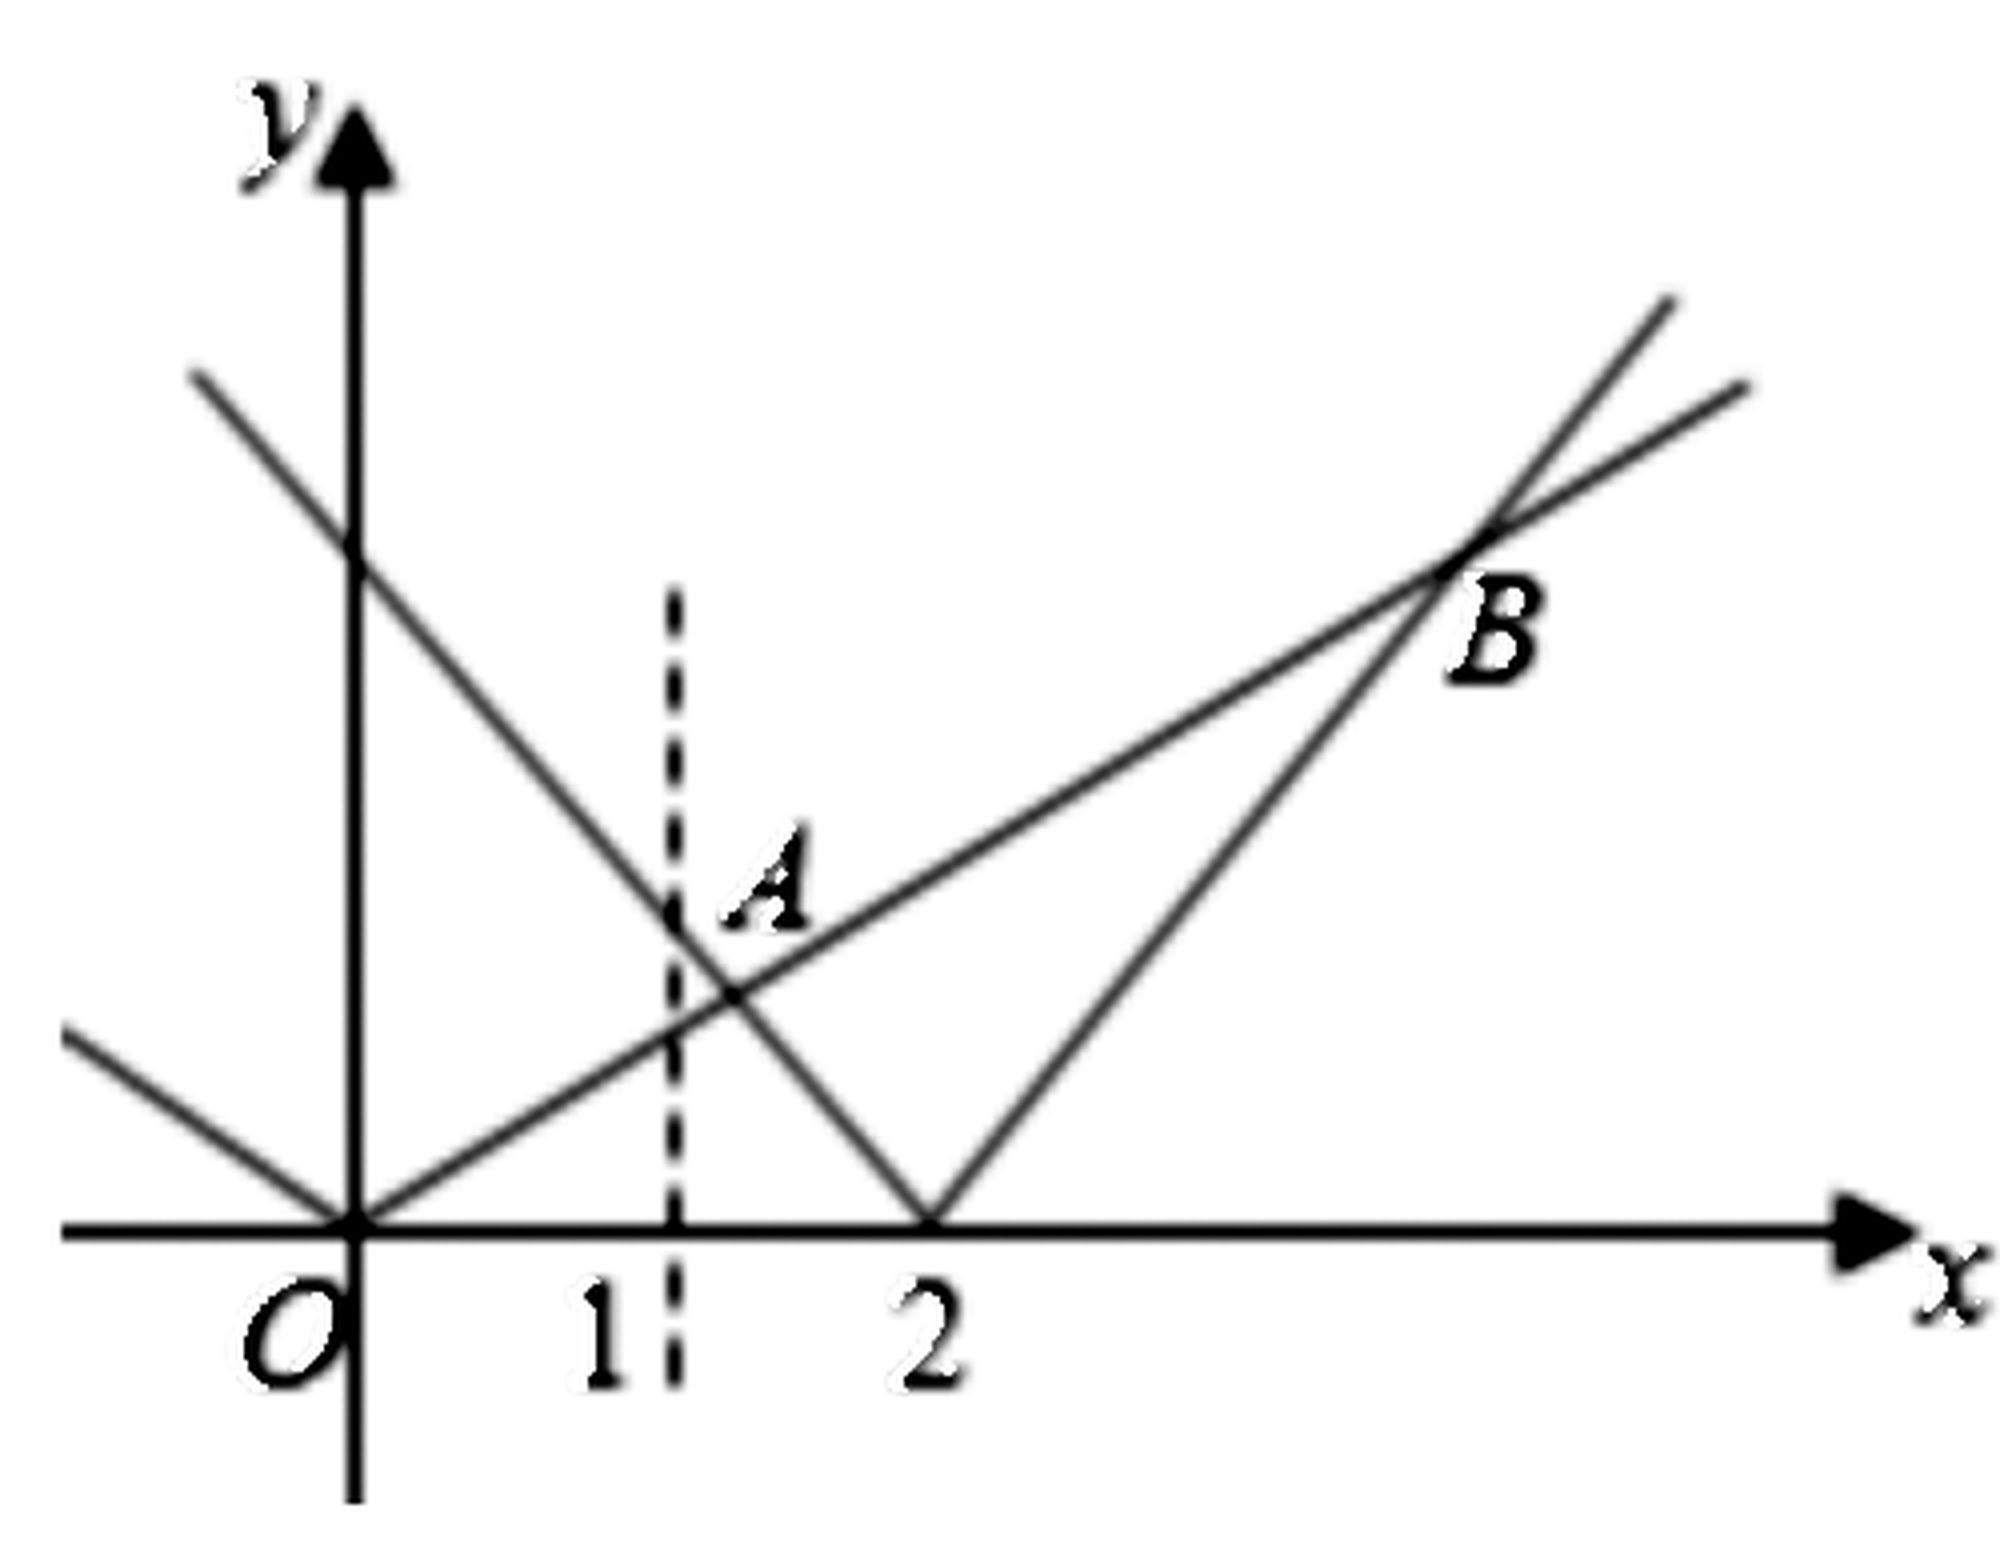
\includegraphics[width=0.40\textwidth]{figures/gao152_q15.png}
\end{center}
\step{由 $0<k<1$，得 $x_A>1$，}
\step{所以关于 $x$ 的不等式 $k\lvert x\rvert-\lvert x-2\rvert>0$ 恰好有 4 个整数解，是 2，3，4，5，}
\step{由 $\begin{cases}y=kx\\y=x-2\end{cases}\Rightarrow x_B=\dfrac2{1-k}\in(5,6]$，故 $\dfrac35<k\leqslant\dfrac23$；故选 $B$.}
\solend
\fi

% === Q16 === 咖啡优惠题；解析 12 行（跨 04 页上下半）；故选 C
\item 上海是全球咖啡店最多的城市. 若某品牌的某种在售咖啡产品价格为 30 元/杯，其原材料成本为 7 元/杯，营销成本为 5 元/杯，且该品牌门店提供如下 4 种优惠方式：(1) 首杯免单，每人限用一次；(2) 3.8 折优惠券，每人限用一次；(3) 买 2 杯送 2 杯，每人限用两次；(4) 买 5 杯送 5 杯，不限使用人数和使用次数. 每位消费者都可以在以上 4 种优惠方式中选择不多于 2 种使用. 现在某个公司有 5 位后勤工作人员去该品牌门店帮每位技术人员购买 1 杯咖啡，购买杯数与技术人员人数须保持一致；请问，这个公司的技术人员不少于\mbox{（\quad）}人时，无论 5 位后勤人员采用什么样的优惠方式购买咖啡，这笔订单该品牌门店都能保证盈利.

\keepwithprev
A. 20\qquad\qquad B. 25\qquad\qquad C. 30\qquad\qquad D. 35

\ifanswer
\solbegin
\step{按各优惠不叠加于同一杯理解，3.8 折券仅用于一杯，}
\step{买赠中的购买杯按原价付款.}
\step{设共购 $n$ 杯，免单、券购、原价购买的杯数分别为 $a,b,c$，其中 $0\leqslant a,b\leqslant5$，}
\step{其余为买赠咖啡，每杯成本为 12 元，}
\step{利润为 $P=15(n-a-b-c)+11.4b+30c-12n=3n-15a-3.6b+15c$，}
\step{若 $a,b$ 不同时为 5，则 $15a+3.6b\leqslant75+14.4=89.4$，}
\step{当 $n\geqslant30$ 时，$P\geqslant90-89.4=0.6>0$.}
\step{若 $a=b=5$，则每人均已使用免单和优惠券两种方式，其余均须原价购买，}
\step{$P=57+30(n-10)-12n=18n-243\geqslant297>0$.}
\step{当 $n=29$ 时，4 人各用方式 (1)(2) 购得 2 杯，}
\step{另 1 人用方式 (1) 及两次方式 (4) 购得 21 杯，}
\step{此时 $P=4\times11.4+2\times150-29\times12=-2.4<0$，因此最小人数为 30，故选 $C$.}% $2\times150$ 为两次方式（4）各买 5 杯的付款，照录（见 ⑤ 3）
\solend
\fi

\end{enumerate}

\bigsec{三、解答题}

\begin{enumerate}
\setcounter{enumi}{16}

% === Q17 === 解集含 \R／\varnothing；解析 4 行
\item 若 $a$、$b\in\R$，求关于 $x$ 的不等式 $ax\geqslant b$ 的解集.

\ifanswer
\solbegin
\step{当 $a>0$ 时，原不等式的解集为 $\left\{x\mid x\geqslant\dfrac ba\right\}$；}
\step{当 $a<0$ 时，原不等式的解集为 $\left\{x\mid x\leqslant\dfrac ba\right\}$；}
\step{当 $a=0$，$b\leqslant0$ 时，原不等式的解集为 $\R$；}
\step{当 $a=0$，$b>0$ 时，原不等式的解集为 $\varnothing$.}
\solend
\fi

% === Q18 === 子集 ⊆ 两处照录；cases 块；解析 9 行（跨 05 页上下半）
\item 已知 $\alpha:x<3m-1$ 或 $x>-m$，$\beta:x<2$ 或 $x\geqslant4$.

(1) 若 $\alpha$ 是 $\beta$ 的充分条件，求实数 $m$ 的取值范围；

(2) 若 $\alpha$ 是 $\beta$ 的必要条件，求实数 $m$ 的取值范围.

\ifanswer
\solbegin
\step{(1) 设 $A=\{x\mid x<3m-1\text{ 或 }x>-m\}$，$B=\{x\mid x<2\text{ 或 }x\geqslant4\}$，}
\step{因为 $\alpha$ 是 $\beta$ 的充分条件，所以 $A\subseteq B$，}
\step{当 $3m-1>-m$ 时，即 $m>\dfrac14$，此时 $A=\R$，不满足题意；}
\step{当 $3m-1\leqslant-m$ 时，即 $m\leqslant\dfrac14$，有 $\begin{cases}3m-1\leqslant2\\-m\geqslant4\end{cases}$，解得 $m\leqslant-4$；}
\step{综上，$m$ 的取值范围为 $(-\infty,-4]$.}
\step{(2) 因为 $\alpha$ 是 $\beta$ 的必要条件，所以 $B\subseteq A$，}
\step{当 $3m-1>-m$ 时，即 $m>\dfrac14$，此时 $A=\R$，$B\subseteq A$ 成立；}
\step{当 $3m-1\leqslant-m$ 时，即 $m\leqslant\dfrac14$，有 $\begin{cases}3m-1\geqslant2\\-m<4\end{cases}$，无解.}
\step{综上，$m$ 的取值范围为 $\left[\dfrac14,+\infty\right)$.}
\solend
\fi

% === Q19 === \varnothing 空集照录；解析 9 行
\item 设关于 $x$ 的不等式 $x^2+4x+k-1\geqslant0$ 的解集为 $A$.

(1) 若 $A=\R$，求实数 $k$ 的取值范围；

(2) 求证：不存在实数 $k$，使得 $A=\varnothing$.

\ifanswer
\solbegin
\step{(1) 配方得 $x^2+4x+k-1=(x+2)^2+k-5$，}
\step{若 $A=\R$，取 $x=-2$，得 $k-5\geqslant0$，即 $k\geqslant5$.}
\step{当 $k\geqslant5$ 时，对任意 $x\in\R$，都有 $(x+2)^2+k-5\geqslant0$，因此 $A=\R$.}
\step{所以 $k$ 的取值范围为 $[5,+\infty)$.}
\step{(2) 当 $k\geqslant5$ 时，由 (1) 得 $A=\R\ne\varnothing$.}
\step{当 $k<5$ 时，取 $x_0=-2+\sqrt{5-k}$，}
\step{则 $x_0^2+4x_0+k-1=(x_0+2)^2+k-5=(5-k)+k-5=0$，}
\step{所以 $x_0\in A$，即 $A\ne\varnothing$.}
\step{因此，不存在实数 $k$，使得 $A=\varnothing$.}
\solend
\fi

% === Q20 === |A\cap B|=1 印等号；等腰偏高粗 \Delta 照录；解析 12 行（跨 06→07 页）
\item 设 $m\in\R$. 集合 $A=\left\{x\mid\dfrac{x^2+x}{x+1}\geqslant\dfrac{2x+m}{x},x\in\R\right\}$，
$B=\left\{x\mid\dfrac{x^2+x}{x+1}\leqslant\dfrac{2x+m}{x},x\in\R\right\}$.

(1) 若 $m=8$，记集合 $M=A\cap(0,+\infty)$，求集合 $M$；

(2) 用 $\lvert T\rvert$ 代表集合 $T$ 的元素个数. 若 $\lvert A\cap B\rvert=1$，记 $m$ 的取值集合为 $C$，试比较 $\lvert C\rvert$ 与 2 的大小，并证明你的结论.

\ifanswer
\solbegin
\step{(1) 当 $m=8$，$x>0$ 时，$\dfrac{x^2+x}{x+1}\geqslant\dfrac{2x+8}{x}\Leftrightarrow x^2-2x-8\geqslant0$}
\step{$\Leftrightarrow(x-4)(x+2)\geqslant0\Leftrightarrow x\geqslant4$，所以 $M=[4,+\infty)$.}
\step{(2) 原分式有意义须 $x\ne-1,0$，因此 $x\in A\cap B\Leftrightarrow\begin{cases}x^2-2x-m=0\\x\ne-1,0\end{cases}$，}
\step{方程的判别式为 $\Delta=4(1+m)$.}
\step{当 $m<-1$ 时，方程无实根，$\lvert A\cap B\rvert=0$；}
\step{当 $m=-1$ 时，方程只有一个实根 1，$A\cap B=\{1\}$.}
\step{当 $m>-1$ 时，方程有两个不同实根.}
\step{其中，0 为根当且仅当 $m=0$，$-1$ 为根当且仅当 $m=3$.}
\step{$m=0$ 时，方程的根为 $0,2$，$A\cap B=\{2\}$；}
\step{$m=3$ 时，方程的根为 $-1,3$，$A\cap B=\{3\}$.}
\step{$m>-1$ 且 $m\ne0,3$ 时，两个实根均满足原分式的定义条件，$\lvert A\cap B\rvert=2$.}
\step{因此 $C=\{-1,0,3\}$，$\lvert C\rvert=3>2$.}
\solend
\fi

% === Q21 === "性质 p"新定义、\Q 归一、M\subseteq\R 照录；解析 19 行（跨 07→08 页）
\item 设集合 $M\subseteq\R$. 若 $M$ 中元素个数大于等于 2，且 $M$ 的任意不同元素 $a$、$b$ 均满足 $a^3-\dfrac14b\in M$，则称集合 $M$ 具有“性质 $p$”.

(1) 试判断集合 $\Q$、集合 $\left\{-\dfrac{\sqrt3}{2},0,\dfrac{\sqrt3}{2}\right\}$ 是否具有“性质 $p$”，并说明理由；

(2) 设 $m$ 为大于等于 2 的正整数. 若集合 $A=\{x_1,x_2,\cdots,x_m\}$，且具有“性质 $p$”，求证：$m=2$，并求集合 $A$ 中所有元素的乘积.

\ifanswer
\solbegin
\step{(1) $\Q$ 中至少有两个元素，且任意不同的 $a,b\in\Q$ 均满足 $a^3-\dfrac14b\in\Q$，}
\step{故 $\Q$ 具有“性质 $p$”.}
\step{对于另一集合，取 $a=0$，$b=\dfrac{\sqrt3}{2}$，则 $a^3-\dfrac14b=-\dfrac{\sqrt3}{8}$ 不属于该集合，}
\step{故其不具有“性质 $p$”.}
\step{(2) 将 $A$ 中元素按 $x_1<x_2<\cdots<x_m$ 排列.}
\step{若 $m\geqslant3$，由性质 $p$ 及幂函数 $y=x^3$ 的单调性，}
\step{有 $x_1^3-\dfrac14x_m<\cdots<x_1^3-\dfrac14x_2<x_m^3-\dfrac14x_2<x_m^3-\dfrac14x_1$，}
\step{上述 $m+1$ 个互不相同的数均属于 $A$，与 $A$ 只有 $m$ 个元素矛盾，}
\step{因此 $m=2$.}
\step{设 $A=\{a,b\}$，$a<b$.}
\step{因为 $a^3-\dfrac14b<b^3-\dfrac14a$，且两者均属于 $A$，}
\step{所以 $a^3-\dfrac14b=a$，$b^3-\dfrac14a=b$，}
\step{两式相减并除以 $a-b\ne0$，}
\step{以及两式相加，分别得 $a^2+ab+b^2=\dfrac34$，$(a+b)(a^2-ab+b^2)=\dfrac54(a+b)$，}
\step{代入 $a^2-ab+b^2=\dfrac34-2ab$，得 $(a+b)(4ab+1)=0$，}
\step{若 $a+b=0$，则 $-ab=a^2+ab+b^2=\dfrac34$，即 $ab=-\dfrac34$；}
\step{若 $a+b\ne0$，则 $ab=-\dfrac14$.}
\step{分别取 $A=\left\{-\dfrac{\sqrt3}{2},\dfrac{\sqrt3}{2}\right\}$，$A=\left\{\dfrac{1-\sqrt3}{2\sqrt2},\dfrac{1+\sqrt3}{2\sqrt2}\right\}$，}
\step{代入均有 $a^3-\dfrac14b=a$、$b^3-\dfrac14a=b$，故两种乘积均可取得.}
\solend
\fi

\end{enumerate}

\end{document}
"
%
% ① 原始材料：微信公众号"魔都数学加油站"文章，连载"27学年高一152"，原文标题
% "27学年高一152——2026-2027年上海市位育中学高一上期中"；
% 原文链接：https://mp.weixin.qq.com/s/v4_G6oTX2BuPz9L-KtLRfw 。
% 正文为 8 张 PNG 页（01/03/05/06/07/08 为 2560×3620，02/04 为 4762×6735，
% 同一篇各页分辨率混排，逐页按各自分辨率裁图核对，别按预览比例换算裁框）。
% 体例：讲评版——填空 3—12（10 题）、选择 13—16（4 题）、解答 17—21（5 题），
% 共 19 题，自第 3 题起编；题目、答案、解析均据原图转录；卷面粉红色水印
% "魔都数学加油站"及公众号页脚未录入。
% 全卷插图清单（逐页通读 8 页确认）：1 幅——第 15 题解析配图（两条折线
% $y=k\lvert x\rvert$ 与 $y=\lvert x-2\rvert$ 及坐标图，03 页右下，含 O、1、2、
% A、B 与虚线 $x=1$），解析写"的图象如下"，仅答案版出，裁
% figures/gao152_q15.png（去粉水印、去色、4× LANCZOS 放大）。
%
% 卷首标题：原卷印作"2026-2027 年位育中学高一上期中"，年份区间按全稿惯例排 en dash；
% 原卷卷面未印副标题，本稿按同期中卷知识模块口径补出"集合与常用逻辑用语、不等式、函数"。
%
% ② 与原卷的排版差异：
%   ① 原文从第 3 题起，本稿保留原题号；共 19 题三节，解答题 5 题到 21；
%   ② 混合体例：第 3、5 题只印【答案】、无【解析】，按 高一140 第 5 题／
%      高一145 第 3 题成例另提 \ans{}、不补造解析；第 13、14 题把答案"D"
%      直接印在题干括号内、题下无【解析】，按 高一84／148／149 成例括号留空、
%      另提 \ans{$D$}；其余 15 题印【解析】、用 \solbegin…\solend；
%      第 15、16 题答案在解析末句"故选 B／C"、括号留空、不另提 \ans{}；
%      答案版【答案】/【解析】标记数 = 19 = 全卷题数（4 个 \ans ＋ 15 个 \solbegin）；
%   ③ 原卷卷面未印副标题，本稿按知识模块口径补出；
%   ④ 原卷填空横线按全稿惯例排 \blankline[4.4em]；选择题括号排 \mbox{（\quad）}、
%      四道选择题的选项段前按惯例各加 \keepwithprev；解答题不留作答区、不加
%      \anspace（原卷为讲评版，109—113 起全稿不用 \anspace）；
%   ⑤ 数集黑板粗体：Q7"全集为 R"、Q9"$\lVert PQ\rVert$ 定义"无数集、
%      Q12"$t\in Z$"、Q13"$k\in Z$ 与 $=\R$"、Q17"$a,b\in R$"、Q19"$A=\R$"、
%      Q20"$m\in\R$"、Q21"$M\subseteq\R$ 与集合 $\Q$"原卷印正体粗体或黑板体
%      R/Q/Z，按全稿惯例归一 \R／\Q／\Z；绝对值排 \lvert…\rvert
%      （Q4、Q9、Q11、Q15），集合描述竖线排 \mid（Q7、Q13、Q20、Q21），
%      距离双竖线排 \lVert…\rVert（Q9 与题干、解析的 ||PQ||／||AB||）；
%      不等号按全稿惯例排 \leqslant／\geqslant；补集照原卷上划线排 \overline{A}
%      （Q7 题干＋解析）；空集 \varnothing（Q17、Q19）；
%      子集 Q18 两处、Q21 题干一处均印带下划线 ⊆、照录 \subseteq（见 ④），
%      本卷无单线 \subset 用例；
%   ⑥ 判别式 Δ/△ 两形混用逐处照录、不得统一：Q11 解析"判别式 △=k²−8k>0"
%      印扁等边细线三角、照录 \triangle，Q20 (2) 解析"判别式为 Δ=4(1+m)"
%      印等腰偏高粗三角、照录 \Delta（/tmp/gao152/z/zoom/q11_delta.png、
%      q20_delta.png 放大并与 151 卷同型并排比较）；
%   ⑦ 中文弯引号照录：Q11"长度"、Q21"性质 p"（题干、两问与解析多处）、
%      Q6 从">"、"<"、"≥"、"≤"中选符号、Q16"（1）…（4）"半角括号；
%      注释里一律 ASCII 引号；数学式内 CJK 用 \text{}（Q13 的"或／且"、
%      Q18 集合描述的"或"）；
%   ⑧ "图像／图象"：全卷仅 Q15 解析一处"的图象如下"，印"图象"（象，无亻）、
%      照录；其余各题无"图像"字样。子题标号 (1)(2)(3)(4) 半角括号照录；
%   ⑨ 半角逗号在数学组之间是全稿惯例、非笔误，逐处照录（Q6、Q10、Q16、
%      Q20、Q21 的 $a,b,c$ 之类）；行末西文句点 ASCII `.`；
%      行中全角逗号／顿号照录（Q11"（a,b）"、Q16"7 元/杯"、Q21"$\Q$、集合"）；
%   ⑩ 复杂式照录别简化：Q4 四组 cases 块（整体各占一个印刷行）、Q8
%      $\frac{x_0}{e^{x_0}}=\frac13$、Q10 $4a^2+b^2=4$、Q12 $b=\frac2a$、
%      Q16 利润式 $P=15(n-a-b-c)+11.4b+30c-12n$、Q18 cases 块、
%      Q20 分式 $\frac{x^2+x}{x+1}$、Q21 $a^3-\frac14b$ 与两组取值集合；
%      \left…\right 不得拆到不同 $…$ 组（Q4 cases 前的 \left\{ 一律改
%      \begin{cases}…\end{cases}、Q17 $\left\{x\mid x\ge\frac ba\right\}$、
%      Q20 $\left\{x\mid\cdots\right\}$、Q21 $\left\{-\frac{\sqrt3}2,\ldots\right\}$）；
%   ⑪ 一条 \step = 原卷解析的一个印刷行，cases 块整体算一个印刷行；别并折行、
%      别拆行。Q12 七行、Q16 十二行、Q18 九行、Q19 九行、Q20 十二行、
%      Q21 十九行均按印刷行逐条断，不丢行；
%   ⑫ 配图：Q15 解析配图（仅答案版出）放 \ifanswer 内 \solbegin…\solend 的
%      \step 之间（高一73 第 16 题／高一150 Q12 成例）；题干无配图，故无
%      \needvspace；
%   ⑬ 原卷解析内无红色"法一／法二"之类小标题，故本卷无 \stepm；红色水印
%      "魔都数学加油站"不录入；
%   ⑭ 跨页续印按题合并：见 ⑥；
%
% ③ 行数复核：一条 \step = 原卷解析的一个印刷行，cases 块作一个印刷行计。
%   逐题数（主会话逐页核对定稿）：Q3：0（只印【答案】、提 \ans{}）；Q4：2；
%   Q5：0（只印【答案】、提 \ans{}）；Q6：1；Q7：1；Q8：1；Q9：1；
%   Q10：4；Q11：5；Q12：7；Q13：0（答案印括号内、提 \ans{}）；
%   Q14：0（答案印括号内、提 \ans{}）；Q15：4；Q16：12；Q17：4；
%   Q18：9；Q19：9；Q20：12；Q21：19。
%   合计 91 条 \step（本卷无 \stepm），与原卷逐题印刷行相等。全卷 15 题设
%   \solbegin…\solend ＋ Q3／Q5／Q13／Q14 四处 \ans{}，答案版
%   【答案】/【解析】标记数 = 19 = 全卷题数。
%
% ④ 判别式／子集符号结论（逐处放大原图照录、不得统一，主会话像素级复核）：
%   判别式：Q11 解析"方程 $x^2-kx+2k=0$ 的判别式 $\triangle=k^2-8k>0$"
%      印扁等边细线三角、照录 \triangle；Q20 (2) 解析"方程的判别式为
%      $\Delta=4(1+m)$"印等腰偏高粗三角、照录 \Delta
%      （/tmp/gao152/z/zoom/q11_delta.png、q20_delta.png；与 高一142／151
%      的"Δ/△ 混用逐处照录"口径一致）。本卷无几何三角形符号。
%   子集：Q18 解析 (1)"$A\subseteq B$"、(2)"$B\subseteq A$"与 Q21 题干
%      "$M\subseteq\R$"共 3 处均印带下划线 ⊆、照录 \subseteq
%      （/tmp/gao152/z/zoom/q18_subset.png、q21_subset.png 放大确认）；
%      本卷无单线 ⊂ 用例。补集上划线 \overline{A}（Q7）、空集 \varnothing
%      （Q17 解析末行、Q19 题干 (2) 与解析）、数集 \R／\Q／\Z 归一见 ② ⑤。
%
% ⑤ 存疑照录（放大原图确认，照录未改、正文对应处另有 % 注）：
%   1. Q11 题干"已知关于 $x$ 的不等式 $x^2-kx+2k<0$ 有实数解，且解集区间
%      长度不超过 3 个单位"，解析据 $\lvert x_1-x_2\rvert\leqslant3$ 推；
%      判别式用扁三角 \triangle（见 ④），照录未改。
%   2. Q12 解析"$t=-1$ 时取 $b=\frac2a\in[-2,-1]$，$c=-1$，则 $ab+c=2-1=1$"
%      ——$b$ 径写 $\frac2a$（无负号），放大 03 页确认，照录未改。
%   3. Q16 解析"$P=4\times11.4+2\times150-29\times12=-2.4<0$"中的
%      $2\times150$ 为两次方式（4）各买 5 杯的付款，照录未改。
%   4. Q20 (2) 题干"若 $\lvert A\cap B\rvert=1$"印等号（非 $\leqslant1$），
%      放大 06 页 /tmp/gao152/z/zoom/q20_eq1.png 确认，照录未改。
%   5. Q21 题干"性质 p"用弯引号且 $p$ 为斜体小写，逐处照录未统一；
%      解析 (2) 末两组 $A$ 的取值集合照录未简化。
%   6. "图像／图象"仅 Q15 一处"图象"、Δ/△ 两形并用（Q11 \triangle、
%      Q20 \Delta）均逐处照录、未统一（见 ② ⑥ ⑧ 与 ④）。
%   全卷除此 6 类外未发现其它笔误／自相矛盾处；19 题中 15 题印【解析】、
%   Q3／Q5 只印【答案】、Q13／Q14 答案印题干括号内（见 ② ②）。
%
% ⑥ 跨页续印按题合并说明（逐页核实定稿）：Q3—Q5 题干＋【答案】／【解析】
%   在 01 页上半，Q6—Q8 题干＋解析在 01 页下半；Q9、Q10 题干＋解析、
%   Q11 题干＋解析、Q12 题干＋解析首行在 02 页；Q12 解析余 6 行续 03 页
%   上半，"二、选择题"标题与 Q13 题干＋选项在 03 页下半；Q13 选项 C／D、
%   Q14 题干＋四选项＋（无解析）、Q15 题干＋四选项＋解析前 3 行＋配图在
%   03 页下半，Q15 解析末行（由 cases 求 $x_B$）续 04 页顶；Q16 题干＋四选项
%   ＋解析前 5 行在 04 页上半，解析余 7 行在 04 页下半；"三、解答题"标题与
%   Q17 题干＋解析首行在 04 页末，Q17 解析余 3 行、Q18 题干＋两问＋解析首
%   4 行在 05 页上半，Q18 解析余 5 行在 05 页下半；Q19 题干＋两问＋解析
%   (1) 4 行在 05—06 页（(2) 题干续 06 页顶），解析 (2) 5 行在 06 页上半；
%   Q20 题干＋两问＋解析 (1) 2 行＋(2) 首行在 06 页下半；Q20 (2) 解析余
%   9 行、Q21 题干＋两问＋解析 (1) 4 行在 07 页；Q21 (2) 解析 19 行中前
%   6 行在 07—08 页上半、末 13 行续 08 页下半，末行"故两种乘积均可取得"
%   为全卷收尾（08 页下半仅水印、无其它正文）。
%   本稿按题连排，不丢行、不并折行；全卷末题为第 21 题，无附加题节。
%
\documentclass[a4paper,11pt]{article}
\usepackage{common}

\begin{document}

\examtitlest[3]{2026--2027 年位育中学高一上期中}{集合与常用逻辑用语、不等式、函数}

\bigsec{一、填空题}

\begin{enumerate}
\setcounter{enumi}{2}

% === Q3 === 原卷只印【答案】、无【解析】，另提 \ans{}，不补造解析
\item 设 $x>0$. 若 $\ln x=-1$，则 $x=$\blankline[4.4em].

\ifanswer
\ans{$\dfrac1{\mathrm{e}}$}
\fi

% === Q4 === 四组 cases 块同一印刷行；解析 2 行
\item 不等式 $\lvert 1-2x\rvert>x$ 的解集为\blankline[4.4em].

\ifanswer
\solbegin
\step{不等式 $\lvert 1-2x\rvert>x$ 即为 $\begin{cases}1-2x\geqslant0\\1-2x>x\end{cases}$ 或 $\begin{cases}1-2x<0\\2x-1>x\end{cases}$，即 $\begin{cases}x\leqslant\frac12\\x<\frac13\end{cases}$ 或 $\begin{cases}x>\frac12\\x>1\end{cases}$，}
\step{则有 $x<\dfrac13$ 或 $x>1$，则解集为 $\left(-\infty,\dfrac13\right)\cup(1,+\infty)$.}
\solend
\fi

% === Q5 === 原卷只印【答案】、无【解析】；\frac1x\ge1 印单线 ≥，按全稿惯例 \geqslant
\item 不等式 $\dfrac1x\geqslant1$ 的解集为\blankline[4.4em].

\ifanswer
\ans{$(0,1]$}
\fi

% === Q6 === 从四个符号中选一个，中文弯引号照录；解析 1 行
\item 设 $a$、$b>0$，则 $a^2+b^2$\blankline[4.4em]$2(2a-b)-5$（从“$>$”、“$<$”、“$\geqslant$”、“$\leqslant$”中选择一个符号填写）.

\ifanswer
\solbegin
\step{$a^2+b^2-[2(2a-b)-5]=(a-2)^2+(b+1)^2>0$，故 $a^2+b^2>2(2a-b)-5$.}
\solend
\fi

% === Q7 === 补集上划线 \overline{A}；集合描述竖线 \mid；解析 1 行
\item 已知全集为 $\R$，集合 $A=\{x\mid y=\sqrt{x-2}\}$，集合 $B=\{y\mid y=\sqrt{x-2}\}$，则 $\overline{A}\cap B=$\blankline[4.4em].

\ifanswer
\solbegin
\step{$A=[2,+\infty)$，$B=[0,+\infty)$，所以 $\overline{A}\cap B=[0,2)$.}
\solend
\fi

% === Q8 === \frac{x_0}{e^{x_0}}=\frac13 照录；解析 1 行
\item 设正数 $x_0$ 满足等式 $\dfrac{x_0}{e^{x_0}}=\dfrac13$，则 $x_0-\ln x_0=$\blankline[4.4em].

\ifanswer
\solbegin
\step{等式两边取自然对数，得 $\ln x_0-x_0=-\ln3$，即 $x_0-\ln x_0=\ln3$.}
\solend
\fi

% === Q9 === 距离双竖线 \lVert…\rVert；解析 1 行
\item 在平面直角坐标系 $xOy$ 中，设点 $P(x_1,y_1)$，$Q(x_2,y_2)$，定义：$\lVert PQ\rVert=\lvert x_1-x_2\rvert+\lvert y_1-y_2\rvert$. 若点 $A(1,0)$，点 $B$ 为直线 $y=x+2$ 上的动点，则 $\lVert AB\rVert$ 的最小值为\blankline[4.4em].

\ifanswer
\solbegin
\step{$\lVert AB\rVert=\lvert x-1\rvert+\lvert y\rvert=\lvert x-1\rvert+\lvert x+2\rvert\geqslant3$，最小值为 3.}
\solend
\fi

% === Q10 === 解析 4 行
\item 已知 $a$、$b$ 均为正数，且 $a^2+\dfrac14b^2=1$，则 $a\sqrt{1+b^2}$ 的最大值为\blankline[4.4em].

\ifanswer
\solbegin
\step{因为 $a$、$b$ 均为正数，且 $a^2+\dfrac14b^2=1$，所以 $4a^2+b^2=4$，}
\step{所以 $a\sqrt{1+b^2}=\dfrac12\cdot2a\cdot\sqrt{1+b^2}\leqslant\dfrac12\cdot\dfrac{4a^2+1+b^2}{2}=\dfrac54$，}
\step{当且仅当 $4a^2=b^2+1$ 即 $a=\dfrac{\sqrt{10}}4$，$b=\dfrac{\sqrt6}2$ 时取等号，}
\step{故 $a\sqrt{1+b^2}$ 的最大值为 $\dfrac54$.}
\solend
\fi

% === Q11 === 扁等边细线判别式 \triangle 照录（见 ④）；"长度"弯引号；解析 5 行
\item 一般地，把 $b-a$ 称为区间 $(a,b)$ 的“长度”. 已知关于 $x$ 的不等式 $x^2-kx+2k<0$ 有实数解，且解集区间长度不超过 3 个单位，则实数 $k$ 的取值范围是\blankline[4.4em].

\ifanswer
\solbegin
\step{因为不等式 $x^2-kx+2k<0$ 有解，}
\step{所以方程 $x^2-kx+2k=0$ 的判别式 $\triangle=k^2-8k>0$，解得 $k>8$ 或 $k<0$，}
\step{由 $x_1+x_2=k$，$x_1x_2=2k$，得 $(x_1-x_2)^2=(x_1+x_2)^2-4x_1x_2=k^2-8k$，}
\step{由 $\lvert x_1-x_2\rvert\leqslant3$，得 $(x_1-x_2)^2\leqslant9$，即 $k^2-8k\leqslant9$，解得 $-1\leqslant k\leqslant9$，}
\step{所以 $-1\leqslant k<0$ 或 $8<k\leqslant9$，即实数 $k$ 的取值范围是 $[-1,0)\cup(8,9]$.}
\solend
\fi

% === Q12 === $b=\frac2a$ 无负号、$c=-1$ 照录（见 ⑤ 2）；解析 7 行（跨 02→03 页）
\item 设 $t\in\Z$，且对任意 $a\in[-2,t]$，总存在 $b,c\in[-2,t]$，使得 $ab+c=1$，则 $t$ 的所有取值为\blankline[4.4em].

\ifanswer
\solbegin
\step{$[-2,t]$ 是区间，要求 $t>-2$，故 $t\geqslant-1$.}
\step{当 $t\geqslant1$ 时，对任意 $a\in[-2,t]$，}
\step{取 $b=0$，$c=1$，两者都属于 $[-2,t]$，且 $ab+c=1$.}
\step{当 $t=0$ 时，取 $a=0$，则 $c=1\notin[-2,0]$，不成立.}
\step{当 $t=-1$ 时，对任意 $a\in[-2,-1]$，取 $b=\dfrac2a\in[-2,-1]$，$c=-1$，}% 原卷径写 $b=\frac2a$（无负号），放大 03 页确认，照录未改（见 ⑤ 2）
\step{则 $ab+c=2-1=1$.}
\step{所以 $t=-1$ 或 $t\geqslant1$（$t\in\Z$）.}
\solend
\fi

\end{enumerate}

\bigsec{二、选择题}

\begin{enumerate}
\setcounter{enumi}{12}

% === Q13 === 答案 D 印在题干括号内、无【解析】，按 高一84／148／149 成例括号留空、另提 \ans{}
\item 下列说法错误的是\mbox{（\quad）}

\keepwithprev
A. 奇数集可以表示为 $\{x\mid x=2k+1,k\in\Z\}$

B. 奇数集可以表示为 $\{x\mid x=2k-1,k\in\Z\}$

C. $\{x\mid x\ne2\text{ 或 }x\ne-2\}=\R$

D. $\{x\mid x\ne2\text{ 且 }x\ne-2\}=\R$

\ifanswer
\ans{$D$}
\fi

% === Q14 === 答案 D 印在题干括号内、无【解析】；选项两行两列
\item 设 $a$、$b$、$c>0$，且 $a\ne1$，则以下代数式中，不恒成立的是\mbox{（\quad）}

\keepwithprev
A. $\log_a 1=0$\qquad\qquad B. $a^{\log_a b}=b$

C. $\log_a b+\log_a c=\log_a(bc)$\qquad\qquad D. $\log_a b=\dfrac1{\log_b a}$

\ifanswer
\ans{$D$}
\fi

% === Q15 === "图象"（象，无亻）照录；解析配图仅答案版出；答案在解析末句故选 B
\item 若关于 $x$ 的不等式 $k\lvert x\rvert>\lvert x-2\rvert$ 恰好有 4 个整数解，则实数 $k$ 的取值范围是\mbox{（\quad）}

\keepwithprev
A. $\left(\dfrac35,\dfrac23\right)$\qquad B. $\left(\dfrac35,\dfrac23\right]$\qquad C. $\left(\dfrac35,1\right)$\qquad D. $\left(\dfrac35,1\right]$

\ifanswer
\solbegin
\step{由题意得 $0<k<1$，函数 $y=k\lvert x\rvert$ 与 $y=\lvert x-2\rvert$ 的图象如下，}
\begin{center}
% 两条折线坐标图取 03 页右下，去粉色水印、去色、4× LANCZOS 放大；仅答案版出
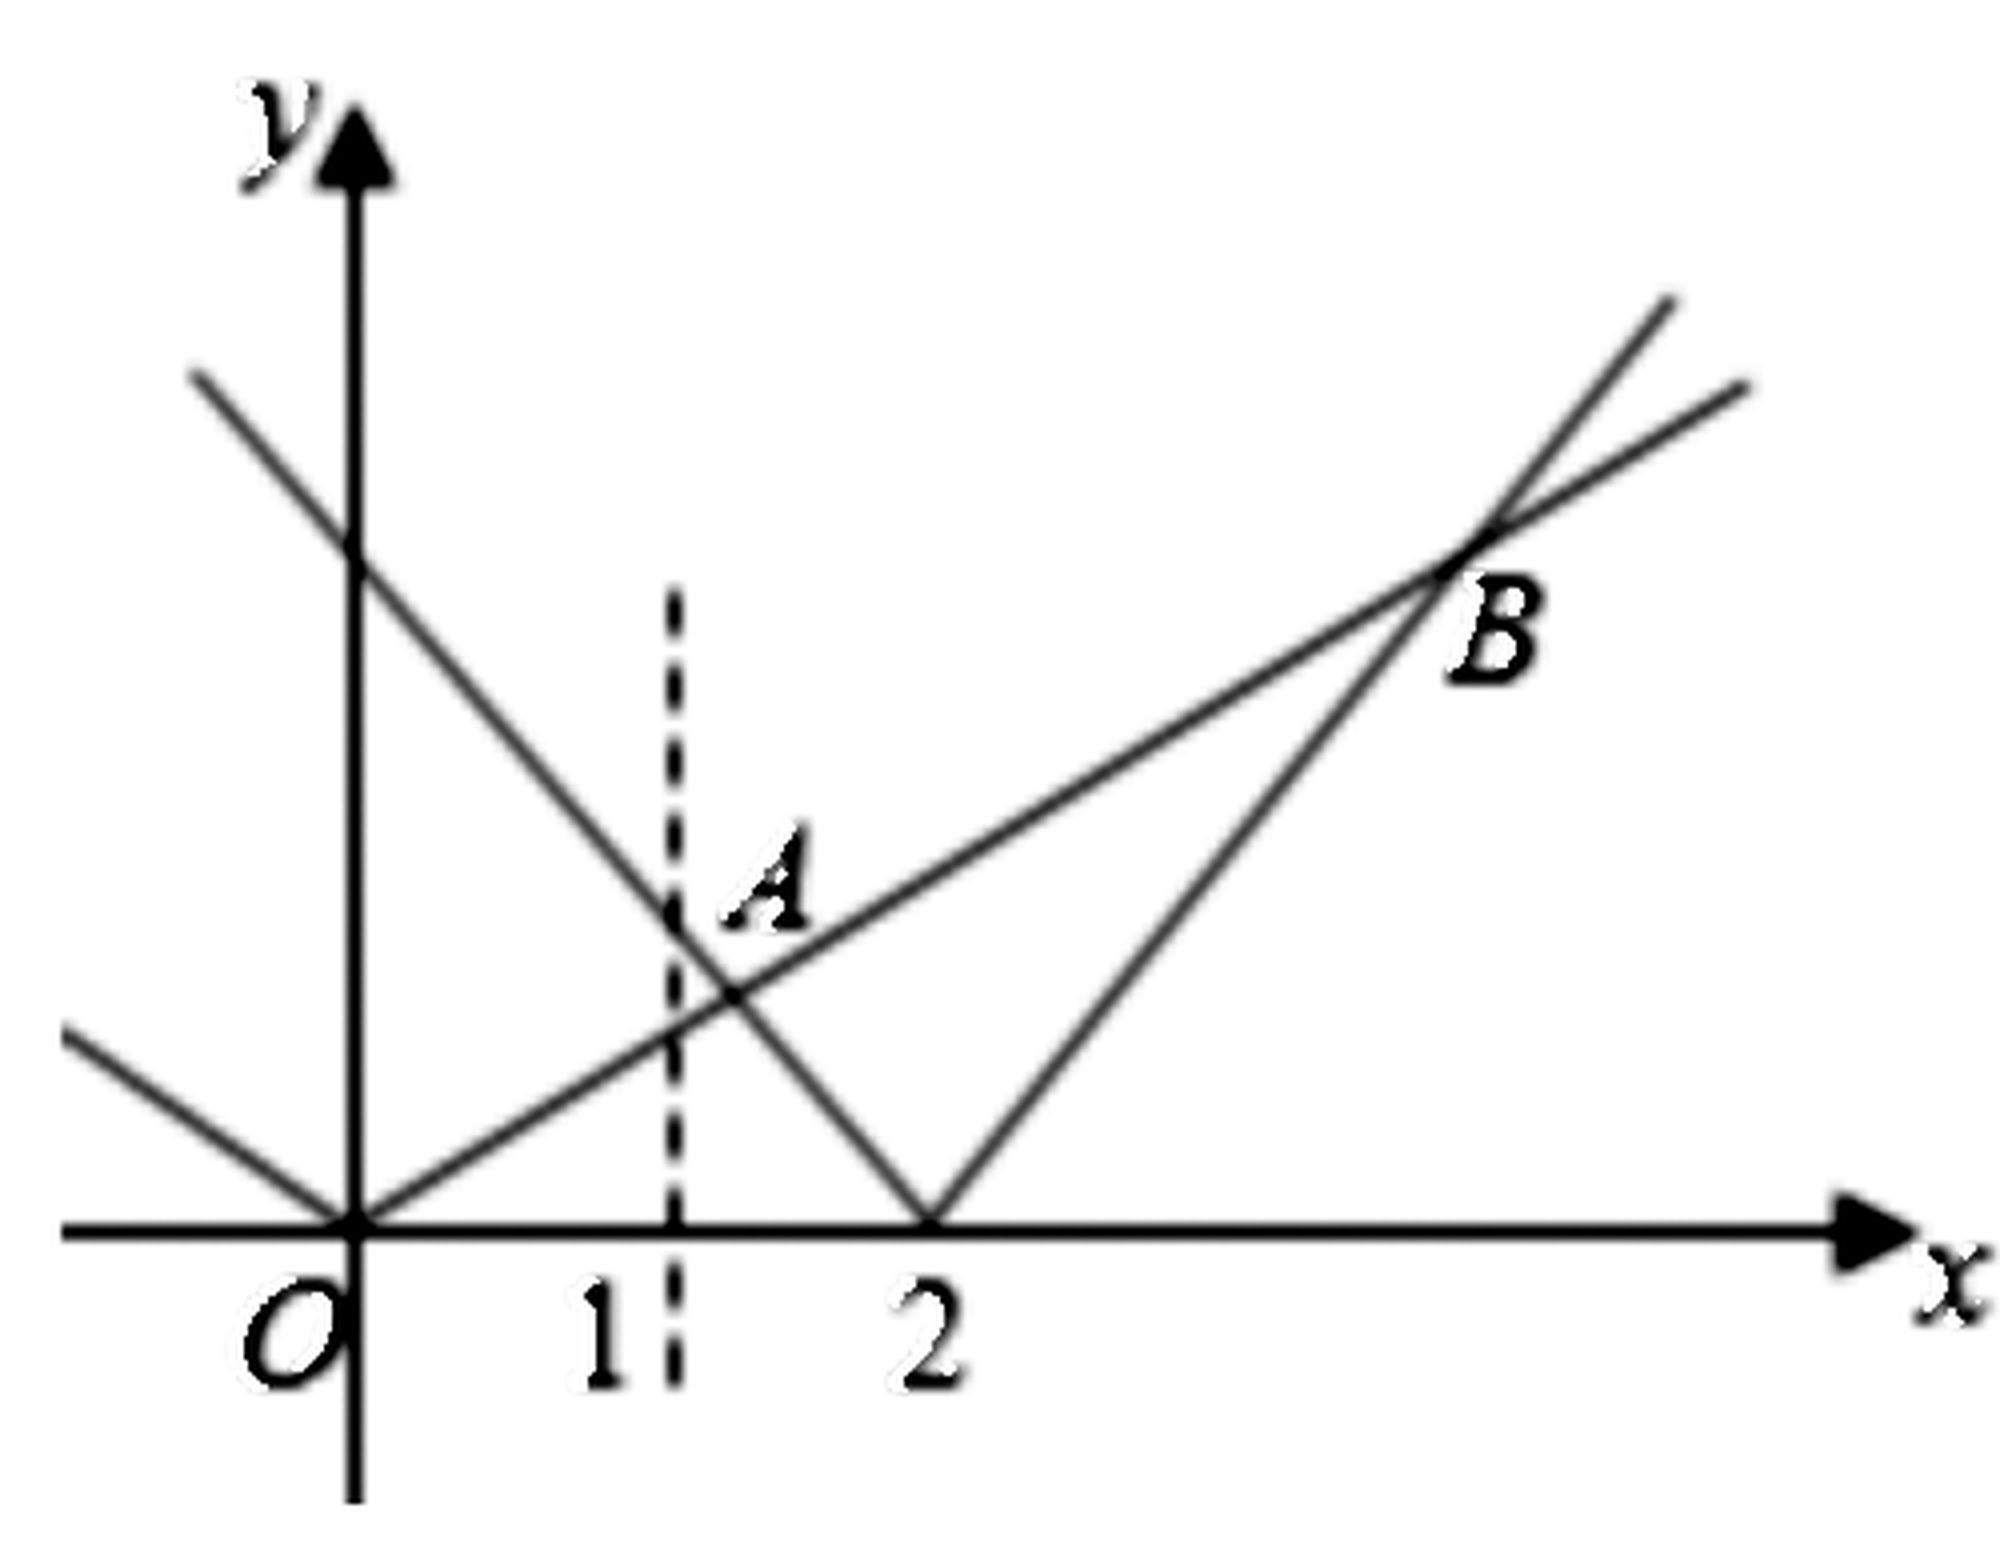
\includegraphics[width=0.40\textwidth]{figures/gao152_q15.png}
\end{center}
\step{由 $0<k<1$，得 $x_A>1$，}
\step{所以关于 $x$ 的不等式 $k\lvert x\rvert-\lvert x-2\rvert>0$ 恰好有 4 个整数解，是 2，3，4，5，}
\step{由 $\begin{cases}y=kx\\y=x-2\end{cases}\Rightarrow x_B=\dfrac2{1-k}\in(5,6]$，故 $\dfrac35<k\leqslant\dfrac23$；故选 $B$.}
\solend
\fi

% === Q16 === 咖啡优惠题；解析 12 行（跨 04 页上下半）；故选 C
\item 上海是全球咖啡店最多的城市. 若某品牌的某种在售咖啡产品价格为 30 元/杯，其原材料成本为 7 元/杯，营销成本为 5 元/杯，且该品牌门店提供如下 4 种优惠方式：(1) 首杯免单，每人限用一次；(2) 3.8 折优惠券，每人限用一次；(3) 买 2 杯送 2 杯，每人限用两次；(4) 买 5 杯送 5 杯，不限使用人数和使用次数. 每位消费者都可以在以上 4 种优惠方式中选择不多于 2 种使用. 现在某个公司有 5 位后勤工作人员去该品牌门店帮每位技术人员购买 1 杯咖啡，购买杯数与技术人员人数须保持一致；请问，这个公司的技术人员不少于\mbox{（\quad）}人时，无论 5 位后勤人员采用什么样的优惠方式购买咖啡，这笔订单该品牌门店都能保证盈利.

\keepwithprev
A. 20\qquad\qquad B. 25\qquad\qquad C. 30\qquad\qquad D. 35

\ifanswer
\solbegin
\step{按各优惠不叠加于同一杯理解，3.8 折券仅用于一杯，}
\step{买赠中的购买杯按原价付款.}
\step{设共购 $n$ 杯，免单、券购、原价购买的杯数分别为 $a,b,c$，其中 $0\leqslant a,b\leqslant5$，}
\step{其余为买赠咖啡，每杯成本为 12 元，}
\step{利润为 $P=15(n-a-b-c)+11.4b+30c-12n=3n-15a-3.6b+15c$，}
\step{若 $a,b$ 不同时为 5，则 $15a+3.6b\leqslant75+14.4=89.4$，}
\step{当 $n\geqslant30$ 时，$P\geqslant90-89.4=0.6>0$.}
\step{若 $a=b=5$，则每人均已使用免单和优惠券两种方式，其余均须原价购买，}
\step{$P=57+30(n-10)-12n=18n-243\geqslant297>0$.}
\step{当 $n=29$ 时，4 人各用方式 (1)(2) 购得 2 杯，}
\step{另 1 人用方式 (1) 及两次方式 (4) 购得 21 杯，}
\step{此时 $P=4\times11.4+2\times150-29\times12=-2.4<0$，因此最小人数为 30，故选 $C$.}% $2\times150$ 为两次方式（4）各买 5 杯的付款，照录（见 ⑤ 3）
\solend
\fi

\end{enumerate}

\bigsec{三、解答题}

\begin{enumerate}
\setcounter{enumi}{16}

% === Q17 === 解集含 \R／\varnothing；解析 4 行
\item 若 $a$、$b\in\R$，求关于 $x$ 的不等式 $ax\geqslant b$ 的解集.

\ifanswer
\solbegin
\step{当 $a>0$ 时，原不等式的解集为 $\left\{x\mid x\geqslant\dfrac ba\right\}$；}
\step{当 $a<0$ 时，原不等式的解集为 $\left\{x\mid x\leqslant\dfrac ba\right\}$；}
\step{当 $a=0$，$b\leqslant0$ 时，原不等式的解集为 $\R$；}
\step{当 $a=0$，$b>0$ 时，原不等式的解集为 $\varnothing$.}
\solend
\fi

% === Q18 === 子集 ⊆ 两处照录；cases 块；解析 9 行（跨 05 页上下半）
\item 已知 $\alpha:x<3m-1$ 或 $x>-m$，$\beta:x<2$ 或 $x\geqslant4$.

(1) 若 $\alpha$ 是 $\beta$ 的充分条件，求实数 $m$ 的取值范围；

(2) 若 $\alpha$ 是 $\beta$ 的必要条件，求实数 $m$ 的取值范围.

\ifanswer
\solbegin
\step{(1) 设 $A=\{x\mid x<3m-1\text{ 或 }x>-m\}$，$B=\{x\mid x<2\text{ 或 }x\geqslant4\}$，}
\step{因为 $\alpha$ 是 $\beta$ 的充分条件，所以 $A\subseteq B$，}
\step{当 $3m-1>-m$ 时，即 $m>\dfrac14$，此时 $A=\R$，不满足题意；}
\step{当 $3m-1\leqslant-m$ 时，即 $m\leqslant\dfrac14$，有 $\begin{cases}3m-1\leqslant2\\-m\geqslant4\end{cases}$，解得 $m\leqslant-4$；}
\step{综上，$m$ 的取值范围为 $(-\infty,-4]$.}
\step{(2) 因为 $\alpha$ 是 $\beta$ 的必要条件，所以 $B\subseteq A$，}
\step{当 $3m-1>-m$ 时，即 $m>\dfrac14$，此时 $A=\R$，$B\subseteq A$ 成立；}
\step{当 $3m-1\leqslant-m$ 时，即 $m\leqslant\dfrac14$，有 $\begin{cases}3m-1\geqslant2\\-m<4\end{cases}$，无解.}
\step{综上，$m$ 的取值范围为 $\left[\dfrac14,+\infty\right)$.}
\solend
\fi

% === Q19 === \varnothing 空集照录；解析 9 行
\item 设关于 $x$ 的不等式 $x^2+4x+k-1\geqslant0$ 的解集为 $A$.

(1) 若 $A=\R$，求实数 $k$ 的取值范围；

(2) 求证：不存在实数 $k$，使得 $A=\varnothing$.

\ifanswer
\solbegin
\step{(1) 配方得 $x^2+4x+k-1=(x+2)^2+k-5$，}
\step{若 $A=\R$，取 $x=-2$，得 $k-5\geqslant0$，即 $k\geqslant5$.}
\step{当 $k\geqslant5$ 时，对任意 $x\in\R$，都有 $(x+2)^2+k-5\geqslant0$，因此 $A=\R$.}
\step{所以 $k$ 的取值范围为 $[5,+\infty)$.}
\step{(2) 当 $k\geqslant5$ 时，由 (1) 得 $A=\R\ne\varnothing$.}
\step{当 $k<5$ 时，取 $x_0=-2+\sqrt{5-k}$，}
\step{则 $x_0^2+4x_0+k-1=(x_0+2)^2+k-5=(5-k)+k-5=0$，}
\step{所以 $x_0\in A$，即 $A\ne\varnothing$.}
\step{因此，不存在实数 $k$，使得 $A=\varnothing$.}
\solend
\fi

% === Q20 === |A\cap B|=1 印等号；等腰偏高粗 \Delta 照录；解析 12 行（跨 06→07 页）
\item 设 $m\in\R$. 集合 $A=\left\{x\mid\dfrac{x^2+x}{x+1}\geqslant\dfrac{2x+m}{x},x\in\R\right\}$，
$B=\left\{x\mid\dfrac{x^2+x}{x+1}\leqslant\dfrac{2x+m}{x},x\in\R\right\}$.

(1) 若 $m=8$，记集合 $M=A\cap(0,+\infty)$，求集合 $M$；

(2) 用 $\lvert T\rvert$ 代表集合 $T$ 的元素个数. 若 $\lvert A\cap B\rvert=1$，记 $m$ 的取值集合为 $C$，试比较 $\lvert C\rvert$ 与 2 的大小，并证明你的结论.

\ifanswer
\solbegin
\step{(1) 当 $m=8$，$x>0$ 时，$\dfrac{x^2+x}{x+1}\geqslant\dfrac{2x+8}{x}\Leftrightarrow x^2-2x-8\geqslant0$}
\step{$\Leftrightarrow(x-4)(x+2)\geqslant0\Leftrightarrow x\geqslant4$，所以 $M=[4,+\infty)$.}
\step{(2) 原分式有意义须 $x\ne-1,0$，因此 $x\in A\cap B\Leftrightarrow\begin{cases}x^2-2x-m=0\\x\ne-1,0\end{cases}$，}
\step{方程的判别式为 $\Delta=4(1+m)$.}
\step{当 $m<-1$ 时，方程无实根，$\lvert A\cap B\rvert=0$；}
\step{当 $m=-1$ 时，方程只有一个实根 1，$A\cap B=\{1\}$.}
\step{当 $m>-1$ 时，方程有两个不同实根.}
\step{其中，0 为根当且仅当 $m=0$，$-1$ 为根当且仅当 $m=3$.}
\step{$m=0$ 时，方程的根为 $0,2$，$A\cap B=\{2\}$；}
\step{$m=3$ 时，方程的根为 $-1,3$，$A\cap B=\{3\}$.}
\step{$m>-1$ 且 $m\ne0,3$ 时，两个实根均满足原分式的定义条件，$\lvert A\cap B\rvert=2$.}
\step{因此 $C=\{-1,0,3\}$，$\lvert C\rvert=3>2$.}
\solend
\fi

% === Q21 === "性质 p"新定义、\Q 归一、M\subseteq\R 照录；解析 19 行（跨 07→08 页）
\item 设集合 $M\subseteq\R$. 若 $M$ 中元素个数大于等于 2，且 $M$ 的任意不同元素 $a$、$b$ 均满足 $a^3-\dfrac14b\in M$，则称集合 $M$ 具有“性质 $p$”.

(1) 试判断集合 $\Q$、集合 $\left\{-\dfrac{\sqrt3}{2},0,\dfrac{\sqrt3}{2}\right\}$ 是否具有“性质 $p$”，并说明理由；

(2) 设 $m$ 为大于等于 2 的正整数. 若集合 $A=\{x_1,x_2,\cdots,x_m\}$，且具有“性质 $p$”，求证：$m=2$，并求集合 $A$ 中所有元素的乘积.

\ifanswer
\solbegin
\step{(1) $\Q$ 中至少有两个元素，且任意不同的 $a,b\in\Q$ 均满足 $a^3-\dfrac14b\in\Q$，}
\step{故 $\Q$ 具有“性质 $p$”.}
\step{对于另一集合，取 $a=0$，$b=\dfrac{\sqrt3}{2}$，则 $a^3-\dfrac14b=-\dfrac{\sqrt3}{8}$ 不属于该集合，}
\step{故其不具有“性质 $p$”.}
\step{(2) 将 $A$ 中元素按 $x_1<x_2<\cdots<x_m$ 排列.}
\step{若 $m\geqslant3$，由性质 $p$ 及幂函数 $y=x^3$ 的单调性，}
\step{有 $x_1^3-\dfrac14x_m<\cdots<x_1^3-\dfrac14x_2<x_m^3-\dfrac14x_2<x_m^3-\dfrac14x_1$，}
\step{上述 $m+1$ 个互不相同的数均属于 $A$，与 $A$ 只有 $m$ 个元素矛盾，}
\step{因此 $m=2$.}
\step{设 $A=\{a,b\}$，$a<b$.}
\step{因为 $a^3-\dfrac14b<b^3-\dfrac14a$，且两者均属于 $A$，}
\step{所以 $a^3-\dfrac14b=a$，$b^3-\dfrac14a=b$，}
\step{两式相减并除以 $a-b\ne0$，}
\step{以及两式相加，分别得 $a^2+ab+b^2=\dfrac34$，$(a+b)(a^2-ab+b^2)=\dfrac54(a+b)$，}
\step{代入 $a^2-ab+b^2=\dfrac34-2ab$，得 $(a+b)(4ab+1)=0$，}
\step{若 $a+b=0$，则 $-ab=a^2+ab+b^2=\dfrac34$，即 $ab=-\dfrac34$；}
\step{若 $a+b\ne0$，则 $ab=-\dfrac14$.}
\step{分别取 $A=\left\{-\dfrac{\sqrt3}{2},\dfrac{\sqrt3}{2}\right\}$，$A=\left\{\dfrac{1-\sqrt3}{2\sqrt2},\dfrac{1+\sqrt3}{2\sqrt2}\right\}$，}
\step{代入均有 $a^3-\dfrac14b=a$、$b^3-\dfrac14a=b$，故两种乘积均可取得.}
\solend
\fi

\end{enumerate}

\end{document}
"
%
% ① 原始材料：微信公众号"魔都数学加油站"文章，连载"27学年高一152"，原文标题
% "27学年高一152——2026-2027年上海市位育中学高一上期中"；
% 原文链接：https://mp.weixin.qq.com/s/v4_G6oTX2BuPz9L-KtLRfw 。
% 正文为 8 张 PNG 页（01/03/05/06/07/08 为 2560×3620，02/04 为 4762×6735，
% 同一篇各页分辨率混排，逐页按各自分辨率裁图核对，别按预览比例换算裁框）。
% 体例：讲评版——填空 3—12（10 题）、选择 13—16（4 题）、解答 17—21（5 题），
% 共 19 题，自第 3 题起编；题目、答案、解析均据原图转录；卷面粉红色水印
% "魔都数学加油站"及公众号页脚未录入。
% 全卷插图清单（逐页通读 8 页确认）：1 幅——第 15 题解析配图（两条折线
% $y=k\lvert x\rvert$ 与 $y=\lvert x-2\rvert$ 及坐标图，03 页右下，含 O、1、2、
% A、B 与虚线 $x=1$），解析写"的图象如下"，仅答案版出，裁
% figures/gao152_q15.png（去粉水印、去色、4× LANCZOS 放大）。
%
% 卷首标题：原卷印作"2026-2027 年位育中学高一上期中"，年份区间按全稿惯例排 en dash；
% 原卷卷面未印副标题，本稿按同期中卷知识模块口径补出"集合与常用逻辑用语、不等式、函数"。
%
% ② 与原卷的排版差异：
%   ① 原文从第 3 题起，本稿保留原题号；共 19 题三节，解答题 5 题到 21；
%   ② 混合体例：第 3、5 题只印【答案】、无【解析】，按 高一140 第 5 题／
%      高一145 第 3 题成例另提 \ans{}、不补造解析；第 13、14 题把答案"D"
%      直接印在题干括号内、题下无【解析】，按 高一84／148／149 成例括号留空、
%      另提 \ans{$D$}；其余 15 题印【解析】、用 \solbegin…\solend；
%      第 15、16 题答案在解析末句"故选 B／C"、括号留空、不另提 \ans{}；
%      答案版【答案】/【解析】标记数 = 19 = 全卷题数（4 个 \ans ＋ 15 个 \solbegin）；
%   ③ 原卷卷面未印副标题，本稿按知识模块口径补出；
%   ④ 原卷填空横线按全稿惯例排 \blankline[4.4em]；选择题括号排 \mbox{（\quad）}、
%      四道选择题的选项段前按惯例各加 \keepwithprev；解答题不留作答区、不加
%      \anspace（原卷为讲评版，109—113 起全稿不用 \anspace）；
%   ⑤ 数集黑板粗体：Q7"全集为 R"、Q9"$\lVert PQ\rVert$ 定义"无数集、
%      Q12"$t\in Z$"、Q13"$k\in Z$ 与 $=\R$"、Q17"$a,b\in R$"、Q19"$A=\R$"、
%      Q20"$m\in\R$"、Q21"$M\subseteq\R$ 与集合 $\Q$"原卷印正体粗体或黑板体
%      R/Q/Z，按全稿惯例归一 \R／\Q／\Z；绝对值排 \lvert…\rvert
%      （Q4、Q9、Q11、Q15），集合描述竖线排 \mid（Q7、Q13、Q20、Q21），
%      距离双竖线排 \lVert…\rVert（Q9 与题干、解析的 ||PQ||／||AB||）；
%      不等号按全稿惯例排 \leqslant／\geqslant；补集照原卷上划线排 \overline{A}
%      （Q7 题干＋解析）；空集 \varnothing（Q17、Q19）；
%      子集 Q18 两处、Q21 题干一处均印带下划线 ⊆、照录 \subseteq（见 ④），
%      本卷无单线 \subset 用例；
%   ⑥ 判别式 Δ/△ 两形混用逐处照录、不得统一：Q11 解析"判别式 △=k²−8k>0"
%      印扁等边细线三角、照录 \triangle，Q20 (2) 解析"判别式为 Δ=4(1+m)"
%      印等腰偏高粗三角、照录 \Delta（/tmp/gao152/z/zoom/q11_delta.png、
%      q20_delta.png 放大并与 151 卷同型并排比较）；
%   ⑦ 中文弯引号照录：Q11"长度"、Q21"性质 p"（题干、两问与解析多处）、
%      Q6 从">"、"<"、"≥"、"≤"中选符号、Q16"（1）…（4）"半角括号；
%      注释里一律 ASCII 引号；数学式内 CJK 用 \text{}（Q13 的"或／且"、
%      Q18 集合描述的"或"）；
%   ⑧ "图像／图象"：全卷仅 Q15 解析一处"的图象如下"，印"图象"（象，无亻）、
%      照录；其余各题无"图像"字样。子题标号 (1)(2)(3)(4) 半角括号照录；
%   ⑨ 半角逗号在数学组之间是全稿惯例、非笔误，逐处照录（Q6、Q10、Q16、
%      Q20、Q21 的 $a,b,c$ 之类）；行末西文句点 ASCII `.`；
%      行中全角逗号／顿号照录（Q11"（a,b）"、Q16"7 元/杯"、Q21"$\Q$、集合"）；
%   ⑩ 复杂式照录别简化：Q4 四组 cases 块（整体各占一个印刷行）、Q8
%      $\frac{x_0}{e^{x_0}}=\frac13$、Q10 $4a^2+b^2=4$、Q12 $b=\frac2a$、
%      Q16 利润式 $P=15(n-a-b-c)+11.4b+30c-12n$、Q18 cases 块、
%      Q20 分式 $\frac{x^2+x}{x+1}$、Q21 $a^3-\frac14b$ 与两组取值集合；
%      \left…\right 不得拆到不同 $…$ 组（Q4 cases 前的 \left\{ 一律改
%      \begin{cases}…\end{cases}、Q17 $\left\{x\mid x\ge\frac ba\right\}$、
%      Q20 $\left\{x\mid\cdots\right\}$、Q21 $\left\{-\frac{\sqrt3}2,\ldots\right\}$）；
%   ⑪ 一条 \step = 原卷解析的一个印刷行，cases 块整体算一个印刷行；别并折行、
%      别拆行。Q12 七行、Q16 十二行、Q18 九行、Q19 九行、Q20 十二行、
%      Q21 十九行均按印刷行逐条断，不丢行；
%   ⑫ 配图：Q15 解析配图（仅答案版出）放 \ifanswer 内 \solbegin…\solend 的
%      \step 之间（高一73 第 16 题／高一150 Q12 成例）；题干无配图，故无
%      \needvspace；
%   ⑬ 原卷解析内无红色"法一／法二"之类小标题，故本卷无 \stepm；红色水印
%      "魔都数学加油站"不录入；
%   ⑭ 跨页续印按题合并：见 ⑥；
%
% ③ 行数复核：一条 \step = 原卷解析的一个印刷行，cases 块作一个印刷行计。
%   逐题数（主会话逐页核对定稿）：Q3：0（只印【答案】、提 \ans{}）；Q4：2；
%   Q5：0（只印【答案】、提 \ans{}）；Q6：1；Q7：1；Q8：1；Q9：1；
%   Q10：4；Q11：5；Q12：7；Q13：0（答案印括号内、提 \ans{}）；
%   Q14：0（答案印括号内、提 \ans{}）；Q15：4；Q16：12；Q17：4；
%   Q18：9；Q19：9；Q20：12；Q21：19。
%   合计 91 条 \step（本卷无 \stepm），与原卷逐题印刷行相等。全卷 15 题设
%   \solbegin…\solend ＋ Q3／Q5／Q13／Q14 四处 \ans{}，答案版
%   【答案】/【解析】标记数 = 19 = 全卷题数。
%
% ④ 判别式／子集符号结论（逐处放大原图照录、不得统一，主会话像素级复核）：
%   判别式：Q11 解析"方程 $x^2-kx+2k=0$ 的判别式 $\triangle=k^2-8k>0$"
%      印扁等边细线三角、照录 \triangle；Q20 (2) 解析"方程的判别式为
%      $\Delta=4(1+m)$"印等腰偏高粗三角、照录 \Delta
%      （/tmp/gao152/z/zoom/q11_delta.png、q20_delta.png；与 高一142／151
%      的"Δ/△ 混用逐处照录"口径一致）。本卷无几何三角形符号。
%   子集：Q18 解析 (1)"$A\subseteq B$"、(2)"$B\subseteq A$"与 Q21 题干
%      "$M\subseteq\R$"共 3 处均印带下划线 ⊆、照录 \subseteq
%      （/tmp/gao152/z/zoom/q18_subset.png、q21_subset.png 放大确认）；
%      本卷无单线 ⊂ 用例。补集上划线 \overline{A}（Q7）、空集 \varnothing
%      （Q17 解析末行、Q19 题干 (2) 与解析）、数集 \R／\Q／\Z 归一见 ② ⑤。
%
% ⑤ 存疑照录（放大原图确认，照录未改、正文对应处另有 % 注）：
%   1. Q11 题干"已知关于 $x$ 的不等式 $x^2-kx+2k<0$ 有实数解，且解集区间
%      长度不超过 3 个单位"，解析据 $\lvert x_1-x_2\rvert\leqslant3$ 推；
%      判别式用扁三角 \triangle（见 ④），照录未改。
%   2. Q12 解析"$t=-1$ 时取 $b=\frac2a\in[-2,-1]$，$c=-1$，则 $ab+c=2-1=1$"
%      ——$b$ 径写 $\frac2a$（无负号），放大 03 页确认，照录未改。
%   3. Q16 解析"$P=4\times11.4+2\times150-29\times12=-2.4<0$"中的
%      $2\times150$ 为两次方式（4）各买 5 杯的付款，照录未改。
%   4. Q20 (2) 题干"若 $\lvert A\cap B\rvert=1$"印等号（非 $\leqslant1$），
%      放大 06 页 /tmp/gao152/z/zoom/q20_eq1.png 确认，照录未改。
%   5. Q21 题干"性质 p"用弯引号且 $p$ 为斜体小写，逐处照录未统一；
%      解析 (2) 末两组 $A$ 的取值集合照录未简化。
%   6. "图像／图象"仅 Q15 一处"图象"、Δ/△ 两形并用（Q11 \triangle、
%      Q20 \Delta）均逐处照录、未统一（见 ② ⑥ ⑧ 与 ④）。
%   全卷除此 6 类外未发现其它笔误／自相矛盾处；19 题中 15 题印【解析】、
%   Q3／Q5 只印【答案】、Q13／Q14 答案印题干括号内（见 ② ②）。
%
% ⑥ 跨页续印按题合并说明（逐页核实定稿）：Q3—Q5 题干＋【答案】／【解析】
%   在 01 页上半，Q6—Q8 题干＋解析在 01 页下半；Q9、Q10 题干＋解析、
%   Q11 题干＋解析、Q12 题干＋解析首行在 02 页；Q12 解析余 6 行续 03 页
%   上半，"二、选择题"标题与 Q13 题干＋选项在 03 页下半；Q13 选项 C／D、
%   Q14 题干＋四选项＋（无解析）、Q15 题干＋四选项＋解析前 3 行＋配图在
%   03 页下半，Q15 解析末行（由 cases 求 $x_B$）续 04 页顶；Q16 题干＋四选项
%   ＋解析前 5 行在 04 页上半，解析余 7 行在 04 页下半；"三、解答题"标题与
%   Q17 题干＋解析首行在 04 页末，Q17 解析余 3 行、Q18 题干＋两问＋解析首
%   4 行在 05 页上半，Q18 解析余 5 行在 05 页下半；Q19 题干＋两问＋解析
%   (1) 4 行在 05—06 页（(2) 题干续 06 页顶），解析 (2) 5 行在 06 页上半；
%   Q20 题干＋两问＋解析 (1) 2 行＋(2) 首行在 06 页下半；Q20 (2) 解析余
%   9 行、Q21 题干＋两问＋解析 (1) 4 行在 07 页；Q21 (2) 解析 19 行中前
%   6 行在 07—08 页上半、末 13 行续 08 页下半，末行"故两种乘积均可取得"
%   为全卷收尾（08 页下半仅水印、无其它正文）。
%   本稿按题连排，不丢行、不并折行；全卷末题为第 21 题，无附加题节。
%
\documentclass[a4paper,11pt]{article}
\usepackage{common}

\begin{document}

\examtitlest[3]{2026--2027 年位育中学高一上期中}{集合与常用逻辑用语、不等式、函数}

\bigsec{一、填空题}

\begin{enumerate}
\setcounter{enumi}{2}

% === Q3 === 原卷只印【答案】、无【解析】，另提 \ans{}，不补造解析
\item 设 $x>0$. 若 $\ln x=-1$，则 $x=$\blankline[4.4em].

\ifanswer
\ans{$\dfrac1{\mathrm{e}}$}
\fi

% === Q4 === 四组 cases 块同一印刷行；解析 2 行
\item 不等式 $\lvert 1-2x\rvert>x$ 的解集为\blankline[4.4em].

\ifanswer
\solbegin
\step{不等式 $\lvert 1-2x\rvert>x$ 即为 $\begin{cases}1-2x\geqslant0\\1-2x>x\end{cases}$ 或 $\begin{cases}1-2x<0\\2x-1>x\end{cases}$，即 $\begin{cases}x\leqslant\frac12\\x<\frac13\end{cases}$ 或 $\begin{cases}x>\frac12\\x>1\end{cases}$，}
\step{则有 $x<\dfrac13$ 或 $x>1$，则解集为 $\left(-\infty,\dfrac13\right)\cup(1,+\infty)$.}
\solend
\fi

% === Q5 === 原卷只印【答案】、无【解析】；\frac1x\ge1 印单线 ≥，按全稿惯例 \geqslant
\item 不等式 $\dfrac1x\geqslant1$ 的解集为\blankline[4.4em].

\ifanswer
\ans{$(0,1]$}
\fi

% === Q6 === 从四个符号中选一个，中文弯引号照录；解析 1 行
\item 设 $a$、$b>0$，则 $a^2+b^2$\blankline[4.4em]$2(2a-b)-5$（从“$>$”、“$<$”、“$\geqslant$”、“$\leqslant$”中选择一个符号填写）.

\ifanswer
\solbegin
\step{$a^2+b^2-[2(2a-b)-5]=(a-2)^2+(b+1)^2>0$，故 $a^2+b^2>2(2a-b)-5$.}
\solend
\fi

% === Q7 === 补集上划线 \overline{A}；集合描述竖线 \mid；解析 1 行
\item 已知全集为 $\R$，集合 $A=\{x\mid y=\sqrt{x-2}\}$，集合 $B=\{y\mid y=\sqrt{x-2}\}$，则 $\overline{A}\cap B=$\blankline[4.4em].

\ifanswer
\solbegin
\step{$A=[2,+\infty)$，$B=[0,+\infty)$，所以 $\overline{A}\cap B=[0,2)$.}
\solend
\fi

% === Q8 === \frac{x_0}{e^{x_0}}=\frac13 照录；解析 1 行
\item 设正数 $x_0$ 满足等式 $\dfrac{x_0}{e^{x_0}}=\dfrac13$，则 $x_0-\ln x_0=$\blankline[4.4em].

\ifanswer
\solbegin
\step{等式两边取自然对数，得 $\ln x_0-x_0=-\ln3$，即 $x_0-\ln x_0=\ln3$.}
\solend
\fi

% === Q9 === 距离双竖线 \lVert…\rVert；解析 1 行
\item 在平面直角坐标系 $xOy$ 中，设点 $P(x_1,y_1)$，$Q(x_2,y_2)$，定义：$\lVert PQ\rVert=\lvert x_1-x_2\rvert+\lvert y_1-y_2\rvert$. 若点 $A(1,0)$，点 $B$ 为直线 $y=x+2$ 上的动点，则 $\lVert AB\rVert$ 的最小值为\blankline[4.4em].

\ifanswer
\solbegin
\step{$\lVert AB\rVert=\lvert x-1\rvert+\lvert y\rvert=\lvert x-1\rvert+\lvert x+2\rvert\geqslant3$，最小值为 3.}
\solend
\fi

% === Q10 === 解析 4 行
\item 已知 $a$、$b$ 均为正数，且 $a^2+\dfrac14b^2=1$，则 $a\sqrt{1+b^2}$ 的最大值为\blankline[4.4em].

\ifanswer
\solbegin
\step{因为 $a$、$b$ 均为正数，且 $a^2+\dfrac14b^2=1$，所以 $4a^2+b^2=4$，}
\step{所以 $a\sqrt{1+b^2}=\dfrac12\cdot2a\cdot\sqrt{1+b^2}\leqslant\dfrac12\cdot\dfrac{4a^2+1+b^2}{2}=\dfrac54$，}
\step{当且仅当 $4a^2=b^2+1$ 即 $a=\dfrac{\sqrt{10}}4$，$b=\dfrac{\sqrt6}2$ 时取等号，}
\step{故 $a\sqrt{1+b^2}$ 的最大值为 $\dfrac54$.}
\solend
\fi

% === Q11 === 扁等边细线判别式 \triangle 照录（见 ④）；"长度"弯引号；解析 5 行
\item 一般地，把 $b-a$ 称为区间 $(a,b)$ 的“长度”. 已知关于 $x$ 的不等式 $x^2-kx+2k<0$ 有实数解，且解集区间长度不超过 3 个单位，则实数 $k$ 的取值范围是\blankline[4.4em].

\ifanswer
\solbegin
\step{因为不等式 $x^2-kx+2k<0$ 有解，}
\step{所以方程 $x^2-kx+2k=0$ 的判别式 $\triangle=k^2-8k>0$，解得 $k>8$ 或 $k<0$，}
\step{由 $x_1+x_2=k$，$x_1x_2=2k$，得 $(x_1-x_2)^2=(x_1+x_2)^2-4x_1x_2=k^2-8k$，}
\step{由 $\lvert x_1-x_2\rvert\leqslant3$，得 $(x_1-x_2)^2\leqslant9$，即 $k^2-8k\leqslant9$，解得 $-1\leqslant k\leqslant9$，}
\step{所以 $-1\leqslant k<0$ 或 $8<k\leqslant9$，即实数 $k$ 的取值范围是 $[-1,0)\cup(8,9]$.}
\solend
\fi

% === Q12 === $b=\frac2a$ 无负号、$c=-1$ 照录（见 ⑤ 2）；解析 7 行（跨 02→03 页）
\item 设 $t\in\Z$，且对任意 $a\in[-2,t]$，总存在 $b,c\in[-2,t]$，使得 $ab+c=1$，则 $t$ 的所有取值为\blankline[4.4em].

\ifanswer
\solbegin
\step{$[-2,t]$ 是区间，要求 $t>-2$，故 $t\geqslant-1$.}
\step{当 $t\geqslant1$ 时，对任意 $a\in[-2,t]$，}
\step{取 $b=0$，$c=1$，两者都属于 $[-2,t]$，且 $ab+c=1$.}
\step{当 $t=0$ 时，取 $a=0$，则 $c=1\notin[-2,0]$，不成立.}
\step{当 $t=-1$ 时，对任意 $a\in[-2,-1]$，取 $b=\dfrac2a\in[-2,-1]$，$c=-1$，}% 原卷径写 $b=\frac2a$（无负号），放大 03 页确认，照录未改（见 ⑤ 2）
\step{则 $ab+c=2-1=1$.}
\step{所以 $t=-1$ 或 $t\geqslant1$（$t\in\Z$）.}
\solend
\fi

\end{enumerate}

\bigsec{二、选择题}

\begin{enumerate}
\setcounter{enumi}{12}

% === Q13 === 答案 D 印在题干括号内、无【解析】，按 高一84／148／149 成例括号留空、另提 \ans{}
\item 下列说法错误的是\mbox{（\quad）}

\keepwithprev
A. 奇数集可以表示为 $\{x\mid x=2k+1,k\in\Z\}$

B. 奇数集可以表示为 $\{x\mid x=2k-1,k\in\Z\}$

C. $\{x\mid x\ne2\text{ 或 }x\ne-2\}=\R$

D. $\{x\mid x\ne2\text{ 且 }x\ne-2\}=\R$

\ifanswer
\ans{$D$}
\fi

% === Q14 === 答案 D 印在题干括号内、无【解析】；选项两行两列
\item 设 $a$、$b$、$c>0$，且 $a\ne1$，则以下代数式中，不恒成立的是\mbox{（\quad）}

\keepwithprev
A. $\log_a 1=0$\qquad\qquad B. $a^{\log_a b}=b$

C. $\log_a b+\log_a c=\log_a(bc)$\qquad\qquad D. $\log_a b=\dfrac1{\log_b a}$

\ifanswer
\ans{$D$}
\fi

% === Q15 === "图象"（象，无亻）照录；解析配图仅答案版出；答案在解析末句故选 B
\item 若关于 $x$ 的不等式 $k\lvert x\rvert>\lvert x-2\rvert$ 恰好有 4 个整数解，则实数 $k$ 的取值范围是\mbox{（\quad）}

\keepwithprev
A. $\left(\dfrac35,\dfrac23\right)$\qquad B. $\left(\dfrac35,\dfrac23\right]$\qquad C. $\left(\dfrac35,1\right)$\qquad D. $\left(\dfrac35,1\right]$

\ifanswer
\solbegin
\step{由题意得 $0<k<1$，函数 $y=k\lvert x\rvert$ 与 $y=\lvert x-2\rvert$ 的图象如下，}
\begin{center}
% 两条折线坐标图取 03 页右下，去粉色水印、去色、4× LANCZOS 放大；仅答案版出
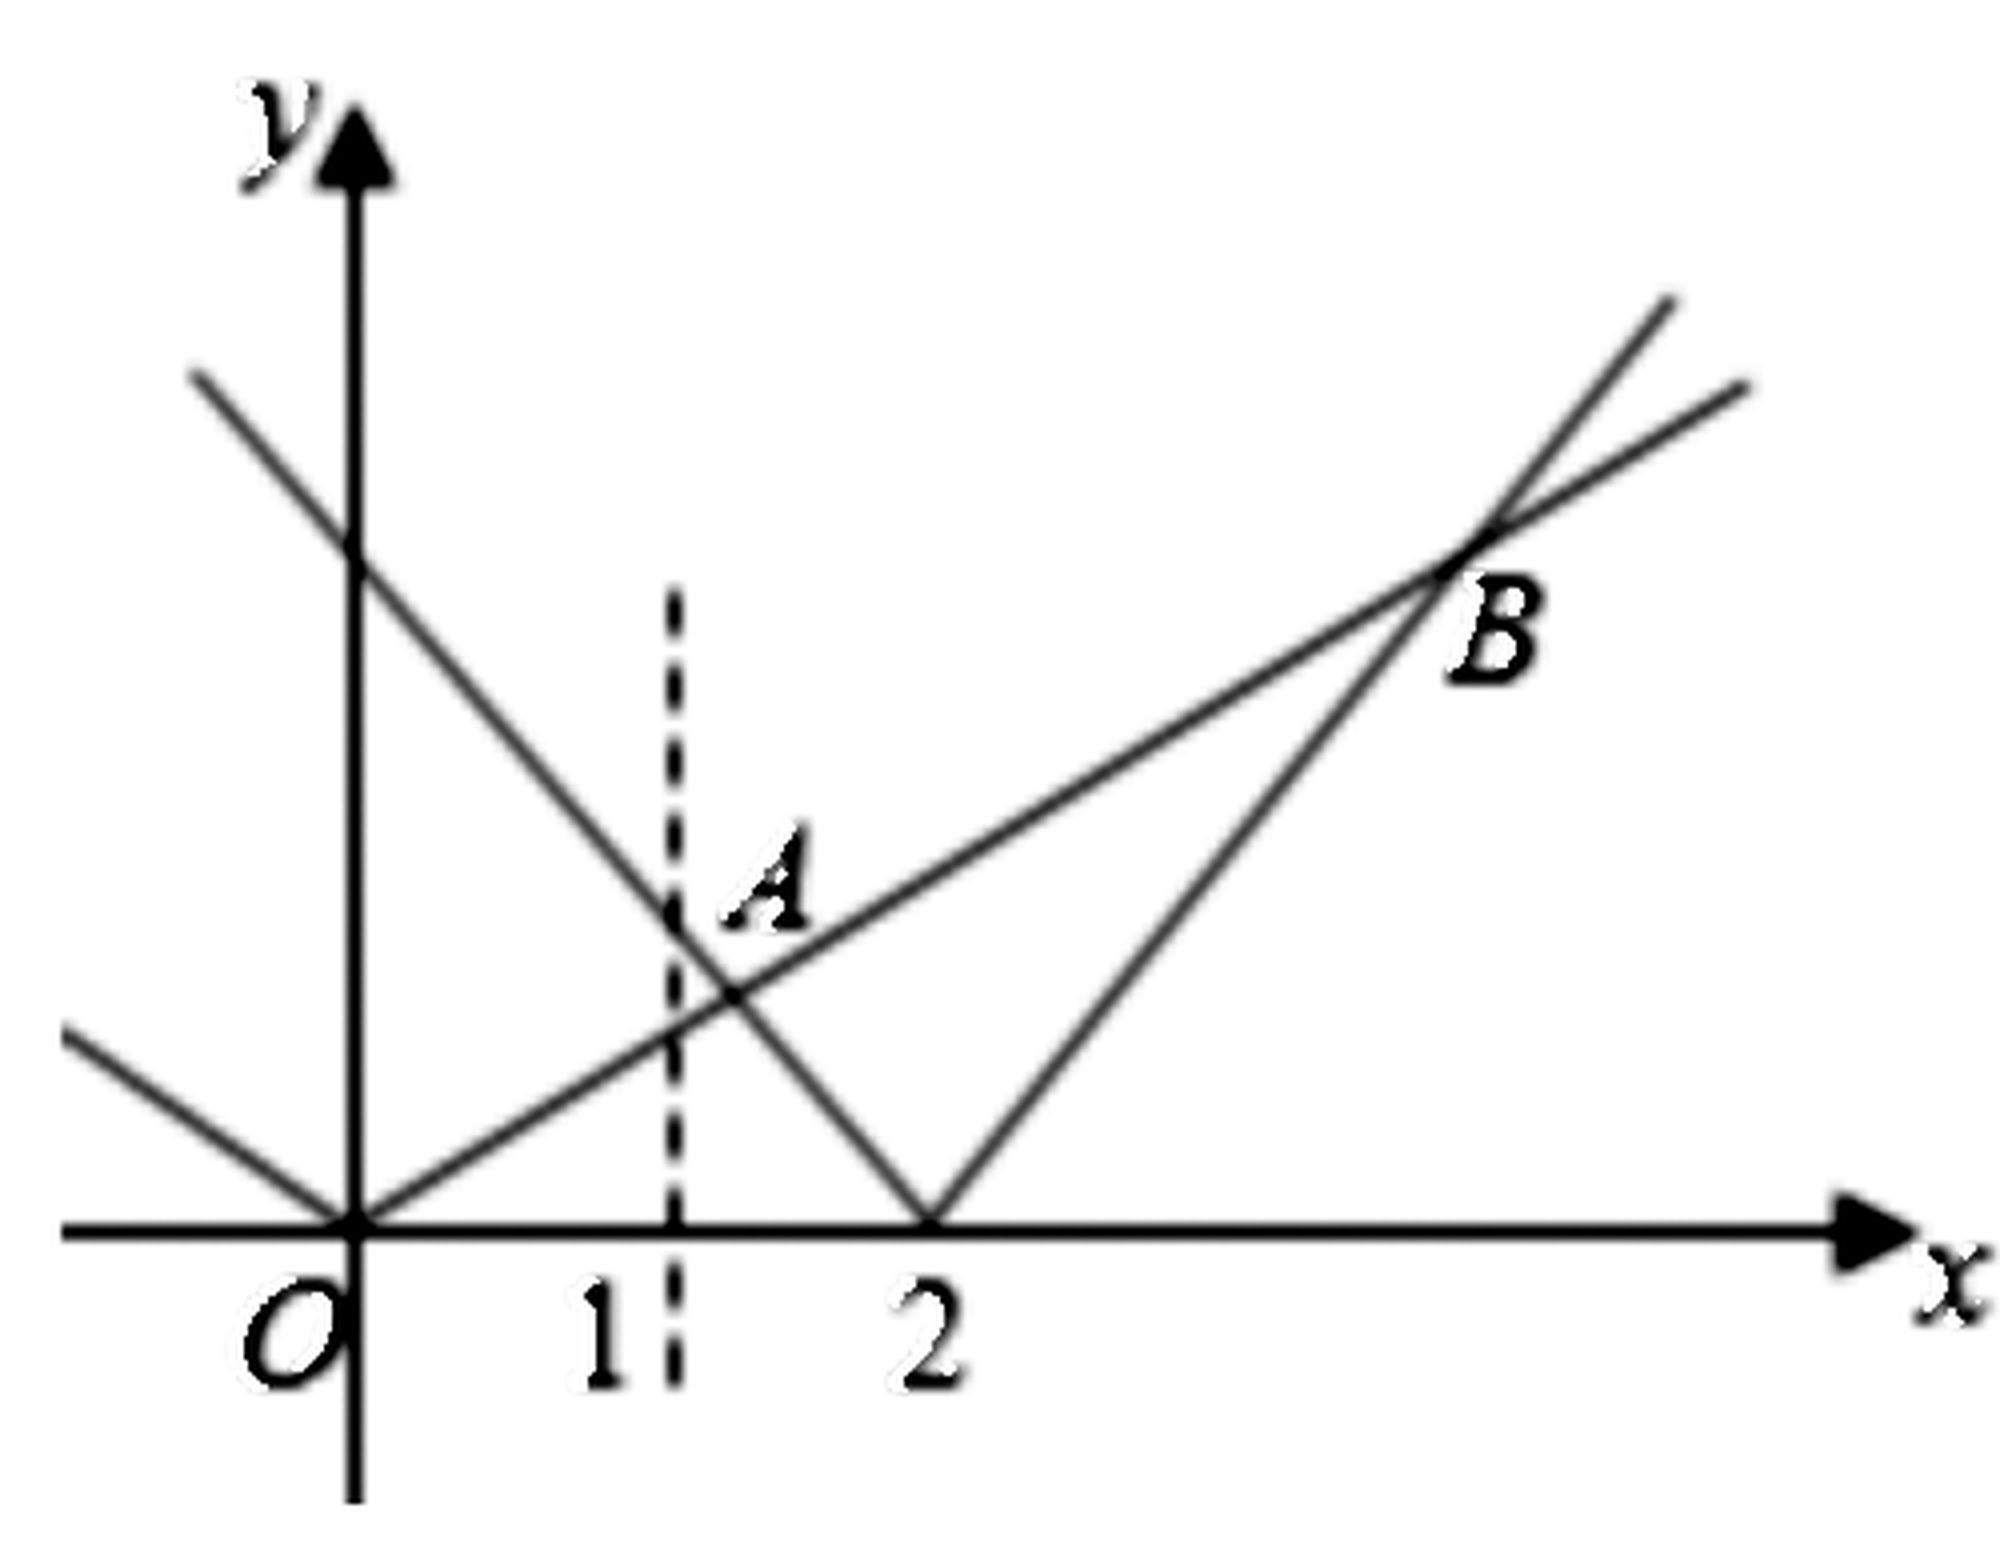
\includegraphics[width=0.40\textwidth]{figures/gao152_q15.png}
\end{center}
\step{由 $0<k<1$，得 $x_A>1$，}
\step{所以关于 $x$ 的不等式 $k\lvert x\rvert-\lvert x-2\rvert>0$ 恰好有 4 个整数解，是 2，3，4，5，}
\step{由 $\begin{cases}y=kx\\y=x-2\end{cases}\Rightarrow x_B=\dfrac2{1-k}\in(5,6]$，故 $\dfrac35<k\leqslant\dfrac23$；故选 $B$.}
\solend
\fi

% === Q16 === 咖啡优惠题；解析 12 行（跨 04 页上下半）；故选 C
\item 上海是全球咖啡店最多的城市. 若某品牌的某种在售咖啡产品价格为 30 元/杯，其原材料成本为 7 元/杯，营销成本为 5 元/杯，且该品牌门店提供如下 4 种优惠方式：(1) 首杯免单，每人限用一次；(2) 3.8 折优惠券，每人限用一次；(3) 买 2 杯送 2 杯，每人限用两次；(4) 买 5 杯送 5 杯，不限使用人数和使用次数. 每位消费者都可以在以上 4 种优惠方式中选择不多于 2 种使用. 现在某个公司有 5 位后勤工作人员去该品牌门店帮每位技术人员购买 1 杯咖啡，购买杯数与技术人员人数须保持一致；请问，这个公司的技术人员不少于\mbox{（\quad）}人时，无论 5 位后勤人员采用什么样的优惠方式购买咖啡，这笔订单该品牌门店都能保证盈利.

\keepwithprev
A. 20\qquad\qquad B. 25\qquad\qquad C. 30\qquad\qquad D. 35

\ifanswer
\solbegin
\step{按各优惠不叠加于同一杯理解，3.8 折券仅用于一杯，}
\step{买赠中的购买杯按原价付款.}
\step{设共购 $n$ 杯，免单、券购、原价购买的杯数分别为 $a,b,c$，其中 $0\leqslant a,b\leqslant5$，}
\step{其余为买赠咖啡，每杯成本为 12 元，}
\step{利润为 $P=15(n-a-b-c)+11.4b+30c-12n=3n-15a-3.6b+15c$，}
\step{若 $a,b$ 不同时为 5，则 $15a+3.6b\leqslant75+14.4=89.4$，}
\step{当 $n\geqslant30$ 时，$P\geqslant90-89.4=0.6>0$.}
\step{若 $a=b=5$，则每人均已使用免单和优惠券两种方式，其余均须原价购买，}
\step{$P=57+30(n-10)-12n=18n-243\geqslant297>0$.}
\step{当 $n=29$ 时，4 人各用方式 (1)(2) 购得 2 杯，}
\step{另 1 人用方式 (1) 及两次方式 (4) 购得 21 杯，}
\step{此时 $P=4\times11.4+2\times150-29\times12=-2.4<0$，因此最小人数为 30，故选 $C$.}% $2\times150$ 为两次方式（4）各买 5 杯的付款，照录（见 ⑤ 3）
\solend
\fi

\end{enumerate}

\bigsec{三、解答题}

\begin{enumerate}
\setcounter{enumi}{16}

% === Q17 === 解集含 \R／\varnothing；解析 4 行
\item 若 $a$、$b\in\R$，求关于 $x$ 的不等式 $ax\geqslant b$ 的解集.

\ifanswer
\solbegin
\step{当 $a>0$ 时，原不等式的解集为 $\left\{x\mid x\geqslant\dfrac ba\right\}$；}
\step{当 $a<0$ 时，原不等式的解集为 $\left\{x\mid x\leqslant\dfrac ba\right\}$；}
\step{当 $a=0$，$b\leqslant0$ 时，原不等式的解集为 $\R$；}
\step{当 $a=0$，$b>0$ 时，原不等式的解集为 $\varnothing$.}
\solend
\fi

% === Q18 === 子集 ⊆ 两处照录；cases 块；解析 9 行（跨 05 页上下半）
\item 已知 $\alpha:x<3m-1$ 或 $x>-m$，$\beta:x<2$ 或 $x\geqslant4$.

(1) 若 $\alpha$ 是 $\beta$ 的充分条件，求实数 $m$ 的取值范围；

(2) 若 $\alpha$ 是 $\beta$ 的必要条件，求实数 $m$ 的取值范围.

\ifanswer
\solbegin
\step{(1) 设 $A=\{x\mid x<3m-1\text{ 或 }x>-m\}$，$B=\{x\mid x<2\text{ 或 }x\geqslant4\}$，}
\step{因为 $\alpha$ 是 $\beta$ 的充分条件，所以 $A\subseteq B$，}
\step{当 $3m-1>-m$ 时，即 $m>\dfrac14$，此时 $A=\R$，不满足题意；}
\step{当 $3m-1\leqslant-m$ 时，即 $m\leqslant\dfrac14$，有 $\begin{cases}3m-1\leqslant2\\-m\geqslant4\end{cases}$，解得 $m\leqslant-4$；}
\step{综上，$m$ 的取值范围为 $(-\infty,-4]$.}
\step{(2) 因为 $\alpha$ 是 $\beta$ 的必要条件，所以 $B\subseteq A$，}
\step{当 $3m-1>-m$ 时，即 $m>\dfrac14$，此时 $A=\R$，$B\subseteq A$ 成立；}
\step{当 $3m-1\leqslant-m$ 时，即 $m\leqslant\dfrac14$，有 $\begin{cases}3m-1\geqslant2\\-m<4\end{cases}$，无解.}
\step{综上，$m$ 的取值范围为 $\left[\dfrac14,+\infty\right)$.}
\solend
\fi

% === Q19 === \varnothing 空集照录；解析 9 行
\item 设关于 $x$ 的不等式 $x^2+4x+k-1\geqslant0$ 的解集为 $A$.

(1) 若 $A=\R$，求实数 $k$ 的取值范围；

(2) 求证：不存在实数 $k$，使得 $A=\varnothing$.

\ifanswer
\solbegin
\step{(1) 配方得 $x^2+4x+k-1=(x+2)^2+k-5$，}
\step{若 $A=\R$，取 $x=-2$，得 $k-5\geqslant0$，即 $k\geqslant5$.}
\step{当 $k\geqslant5$ 时，对任意 $x\in\R$，都有 $(x+2)^2+k-5\geqslant0$，因此 $A=\R$.}
\step{所以 $k$ 的取值范围为 $[5,+\infty)$.}
\step{(2) 当 $k\geqslant5$ 时，由 (1) 得 $A=\R\ne\varnothing$.}
\step{当 $k<5$ 时，取 $x_0=-2+\sqrt{5-k}$，}
\step{则 $x_0^2+4x_0+k-1=(x_0+2)^2+k-5=(5-k)+k-5=0$，}
\step{所以 $x_0\in A$，即 $A\ne\varnothing$.}
\step{因此，不存在实数 $k$，使得 $A=\varnothing$.}
\solend
\fi

% === Q20 === |A\cap B|=1 印等号；等腰偏高粗 \Delta 照录；解析 12 行（跨 06→07 页）
\item 设 $m\in\R$. 集合 $A=\left\{x\mid\dfrac{x^2+x}{x+1}\geqslant\dfrac{2x+m}{x},x\in\R\right\}$，
$B=\left\{x\mid\dfrac{x^2+x}{x+1}\leqslant\dfrac{2x+m}{x},x\in\R\right\}$.

(1) 若 $m=8$，记集合 $M=A\cap(0,+\infty)$，求集合 $M$；

(2) 用 $\lvert T\rvert$ 代表集合 $T$ 的元素个数. 若 $\lvert A\cap B\rvert=1$，记 $m$ 的取值集合为 $C$，试比较 $\lvert C\rvert$ 与 2 的大小，并证明你的结论.

\ifanswer
\solbegin
\step{(1) 当 $m=8$，$x>0$ 时，$\dfrac{x^2+x}{x+1}\geqslant\dfrac{2x+8}{x}\Leftrightarrow x^2-2x-8\geqslant0$}
\step{$\Leftrightarrow(x-4)(x+2)\geqslant0\Leftrightarrow x\geqslant4$，所以 $M=[4,+\infty)$.}
\step{(2) 原分式有意义须 $x\ne-1,0$，因此 $x\in A\cap B\Leftrightarrow\begin{cases}x^2-2x-m=0\\x\ne-1,0\end{cases}$，}
\step{方程的判别式为 $\Delta=4(1+m)$.}
\step{当 $m<-1$ 时，方程无实根，$\lvert A\cap B\rvert=0$；}
\step{当 $m=-1$ 时，方程只有一个实根 1，$A\cap B=\{1\}$.}
\step{当 $m>-1$ 时，方程有两个不同实根.}
\step{其中，0 为根当且仅当 $m=0$，$-1$ 为根当且仅当 $m=3$.}
\step{$m=0$ 时，方程的根为 $0,2$，$A\cap B=\{2\}$；}
\step{$m=3$ 时，方程的根为 $-1,3$，$A\cap B=\{3\}$.}
\step{$m>-1$ 且 $m\ne0,3$ 时，两个实根均满足原分式的定义条件，$\lvert A\cap B\rvert=2$.}
\step{因此 $C=\{-1,0,3\}$，$\lvert C\rvert=3>2$.}
\solend
\fi

% === Q21 === "性质 p"新定义、\Q 归一、M\subseteq\R 照录；解析 19 行（跨 07→08 页）
\item 设集合 $M\subseteq\R$. 若 $M$ 中元素个数大于等于 2，且 $M$ 的任意不同元素 $a$、$b$ 均满足 $a^3-\dfrac14b\in M$，则称集合 $M$ 具有“性质 $p$”.

(1) 试判断集合 $\Q$、集合 $\left\{-\dfrac{\sqrt3}{2},0,\dfrac{\sqrt3}{2}\right\}$ 是否具有“性质 $p$”，并说明理由；

(2) 设 $m$ 为大于等于 2 的正整数. 若集合 $A=\{x_1,x_2,\cdots,x_m\}$，且具有“性质 $p$”，求证：$m=2$，并求集合 $A$ 中所有元素的乘积.

\ifanswer
\solbegin
\step{(1) $\Q$ 中至少有两个元素，且任意不同的 $a,b\in\Q$ 均满足 $a^3-\dfrac14b\in\Q$，}
\step{故 $\Q$ 具有“性质 $p$”.}
\step{对于另一集合，取 $a=0$，$b=\dfrac{\sqrt3}{2}$，则 $a^3-\dfrac14b=-\dfrac{\sqrt3}{8}$ 不属于该集合，}
\step{故其不具有“性质 $p$”.}
\step{(2) 将 $A$ 中元素按 $x_1<x_2<\cdots<x_m$ 排列.}
\step{若 $m\geqslant3$，由性质 $p$ 及幂函数 $y=x^3$ 的单调性，}
\step{有 $x_1^3-\dfrac14x_m<\cdots<x_1^3-\dfrac14x_2<x_m^3-\dfrac14x_2<x_m^3-\dfrac14x_1$，}
\step{上述 $m+1$ 个互不相同的数均属于 $A$，与 $A$ 只有 $m$ 个元素矛盾，}
\step{因此 $m=2$.}
\step{设 $A=\{a,b\}$，$a<b$.}
\step{因为 $a^3-\dfrac14b<b^3-\dfrac14a$，且两者均属于 $A$，}
\step{所以 $a^3-\dfrac14b=a$，$b^3-\dfrac14a=b$，}
\step{两式相减并除以 $a-b\ne0$，}
\step{以及两式相加，分别得 $a^2+ab+b^2=\dfrac34$，$(a+b)(a^2-ab+b^2)=\dfrac54(a+b)$，}
\step{代入 $a^2-ab+b^2=\dfrac34-2ab$，得 $(a+b)(4ab+1)=0$，}
\step{若 $a+b=0$，则 $-ab=a^2+ab+b^2=\dfrac34$，即 $ab=-\dfrac34$；}
\step{若 $a+b\ne0$，则 $ab=-\dfrac14$.}
\step{分别取 $A=\left\{-\dfrac{\sqrt3}{2},\dfrac{\sqrt3}{2}\right\}$，$A=\left\{\dfrac{1-\sqrt3}{2\sqrt2},\dfrac{1+\sqrt3}{2\sqrt2}\right\}$，}
\step{代入均有 $a^3-\dfrac14b=a$、$b^3-\dfrac14a=b$，故两种乘积均可取得.}
\solend
\fi

\end{enumerate}

\end{document}
"
%
% ① 原始材料：微信公众号"魔都数学加油站"文章，连载"27学年高一152"，原文标题
% "27学年高一152——2026-2027年上海市位育中学高一上期中"；
% 原文链接：https://mp.weixin.qq.com/s/v4_G6oTX2BuPz9L-KtLRfw 。
% 正文为 8 张 PNG 页（01/03/05/06/07/08 为 2560×3620，02/04 为 4762×6735，
% 同一篇各页分辨率混排，逐页按各自分辨率裁图核对，别按预览比例换算裁框）。
% 体例：讲评版——填空 3—12（10 题）、选择 13—16（4 题）、解答 17—21（5 题），
% 共 19 题，自第 3 题起编；题目、答案、解析均据原图转录；卷面粉红色水印
% "魔都数学加油站"及公众号页脚未录入。
% 全卷插图清单（逐页通读 8 页确认）：1 幅——第 15 题解析配图（两条折线
% $y=k\lvert x\rvert$ 与 $y=\lvert x-2\rvert$ 及坐标图，03 页右下，含 O、1、2、
% A、B 与虚线 $x=1$），解析写"的图象如下"，仅答案版出，裁
% figures/gao152_q15.png（去粉水印、去色、4× LANCZOS 放大）。
%
% 卷首标题：原卷印作"2026-2027 年位育中学高一上期中"，年份区间按全稿惯例排 en dash；
% 原卷卷面未印副标题，本稿按同期中卷知识模块口径补出"集合与常用逻辑用语、不等式、函数"。
%
% ② 与原卷的排版差异：
%   ① 原文从第 3 题起，本稿保留原题号；共 19 题三节，解答题 5 题到 21；
%   ② 混合体例：第 3、5 题只印【答案】、无【解析】，按 高一140 第 5 题／
%      高一145 第 3 题成例另提 \ans{}、不补造解析；第 13、14 题把答案"D"
%      直接印在题干括号内、题下无【解析】，按 高一84／148／149 成例括号留空、
%      另提 \ans{$D$}；其余 15 题印【解析】、用 \solbegin…\solend；
%      第 15、16 题答案在解析末句"故选 B／C"、括号留空、不另提 \ans{}；
%      答案版【答案】/【解析】标记数 = 19 = 全卷题数（4 个 \ans ＋ 15 个 \solbegin）；
%   ③ 原卷卷面未印副标题，本稿按知识模块口径补出；
%   ④ 原卷填空横线按全稿惯例排 \blankline[4.4em]；选择题括号排 \mbox{（\quad）}、
%      四道选择题的选项段前按惯例各加 \keepwithprev；解答题不留作答区、不加
%      \anspace（原卷为讲评版，109—113 起全稿不用 \anspace）；
%   ⑤ 数集黑板粗体：Q7"全集为 R"、Q9"$\lVert PQ\rVert$ 定义"无数集、
%      Q12"$t\in Z$"、Q13"$k\in Z$ 与 $=\R$"、Q17"$a,b\in R$"、Q19"$A=\R$"、
%      Q20"$m\in\R$"、Q21"$M\subseteq\R$ 与集合 $\Q$"原卷印正体粗体或黑板体
%      R/Q/Z，按全稿惯例归一 \R／\Q／\Z；绝对值排 \lvert…\rvert
%      （Q4、Q9、Q11、Q15），集合描述竖线排 \mid（Q7、Q13、Q20、Q21），
%      距离双竖线排 \lVert…\rVert（Q9 与题干、解析的 ||PQ||／||AB||）；
%      不等号按全稿惯例排 \leqslant／\geqslant；补集照原卷上划线排 \overline{A}
%      （Q7 题干＋解析）；空集 \varnothing（Q17、Q19）；
%      子集 Q18 两处、Q21 题干一处均印带下划线 ⊆、照录 \subseteq（见 ④），
%      本卷无单线 \subset 用例；
%   ⑥ 判别式 Δ/△ 两形混用逐处照录、不得统一：Q11 解析"判别式 △=k²−8k>0"
%      印扁等边细线三角、照录 \triangle，Q20 (2) 解析"判别式为 Δ=4(1+m)"
%      印等腰偏高粗三角、照录 \Delta（/tmp/gao152/z/zoom/q11_delta.png、
%      q20_delta.png 放大并与 151 卷同型并排比较）；
%   ⑦ 中文弯引号照录：Q11"长度"、Q21"性质 p"（题干、两问与解析多处）、
%      Q6 从">"、"<"、"≥"、"≤"中选符号、Q16"（1）…（4）"半角括号；
%      注释里一律 ASCII 引号；数学式内 CJK 用 \text{}（Q13 的"或／且"、
%      Q18 集合描述的"或"）；
%   ⑧ "图像／图象"：全卷仅 Q15 解析一处"的图象如下"，印"图象"（象，无亻）、
%      照录；其余各题无"图像"字样。子题标号 (1)(2)(3)(4) 半角括号照录；
%   ⑨ 半角逗号在数学组之间是全稿惯例、非笔误，逐处照录（Q6、Q10、Q16、
%      Q20、Q21 的 $a,b,c$ 之类）；行末西文句点 ASCII `.`；
%      行中全角逗号／顿号照录（Q11"（a,b）"、Q16"7 元/杯"、Q21"$\Q$、集合"）；
%   ⑩ 复杂式照录别简化：Q4 四组 cases 块（整体各占一个印刷行）、Q8
%      $\frac{x_0}{e^{x_0}}=\frac13$、Q10 $4a^2+b^2=4$、Q12 $b=\frac2a$、
%      Q16 利润式 $P=15(n-a-b-c)+11.4b+30c-12n$、Q18 cases 块、
%      Q20 分式 $\frac{x^2+x}{x+1}$、Q21 $a^3-\frac14b$ 与两组取值集合；
%      \left…\right 不得拆到不同 $…$ 组（Q4 cases 前的 \left\{ 一律改
%      \begin{cases}…\end{cases}、Q17 $\left\{x\mid x\ge\frac ba\right\}$、
%      Q20 $\left\{x\mid\cdots\right\}$、Q21 $\left\{-\frac{\sqrt3}2,\ldots\right\}$）；
%   ⑪ 一条 \step = 原卷解析的一个印刷行，cases 块整体算一个印刷行；别并折行、
%      别拆行。Q12 七行、Q16 十二行、Q18 九行、Q19 九行、Q20 十二行、
%      Q21 十九行均按印刷行逐条断，不丢行；
%   ⑫ 配图：Q15 解析配图（仅答案版出）放 \ifanswer 内 \solbegin…\solend 的
%      \step 之间（高一73 第 16 题／高一150 Q12 成例）；题干无配图，故无
%      \needvspace；
%   ⑬ 原卷解析内无红色"法一／法二"之类小标题，故本卷无 \stepm；红色水印
%      "魔都数学加油站"不录入；
%   ⑭ 跨页续印按题合并：见 ⑥；
%
% ③ 行数复核：一条 \step = 原卷解析的一个印刷行，cases 块作一个印刷行计。
%   逐题数（主会话逐页核对定稿）：Q3：0（只印【答案】、提 \ans{}）；Q4：2；
%   Q5：0（只印【答案】、提 \ans{}）；Q6：1；Q7：1；Q8：1；Q9：1；
%   Q10：4；Q11：5；Q12：7；Q13：0（答案印括号内、提 \ans{}）；
%   Q14：0（答案印括号内、提 \ans{}）；Q15：4；Q16：12；Q17：4；
%   Q18：9；Q19：9；Q20：12；Q21：19。
%   合计 91 条 \step（本卷无 \stepm），与原卷逐题印刷行相等。全卷 15 题设
%   \solbegin…\solend ＋ Q3／Q5／Q13／Q14 四处 \ans{}，答案版
%   【答案】/【解析】标记数 = 19 = 全卷题数。
%
% ④ 判别式／子集符号结论（逐处放大原图照录、不得统一，主会话像素级复核）：
%   判别式：Q11 解析"方程 $x^2-kx+2k=0$ 的判别式 $\triangle=k^2-8k>0$"
%      印扁等边细线三角、照录 \triangle；Q20 (2) 解析"方程的判别式为
%      $\Delta=4(1+m)$"印等腰偏高粗三角、照录 \Delta
%      （/tmp/gao152/z/zoom/q11_delta.png、q20_delta.png；与 高一142／151
%      的"Δ/△ 混用逐处照录"口径一致）。本卷无几何三角形符号。
%   子集：Q18 解析 (1)"$A\subseteq B$"、(2)"$B\subseteq A$"与 Q21 题干
%      "$M\subseteq\R$"共 3 处均印带下划线 ⊆、照录 \subseteq
%      （/tmp/gao152/z/zoom/q18_subset.png、q21_subset.png 放大确认）；
%      本卷无单线 ⊂ 用例。补集上划线 \overline{A}（Q7）、空集 \varnothing
%      （Q17 解析末行、Q19 题干 (2) 与解析）、数集 \R／\Q／\Z 归一见 ② ⑤。
%
% ⑤ 存疑照录（放大原图确认，照录未改、正文对应处另有 % 注）：
%   1. Q11 题干"已知关于 $x$ 的不等式 $x^2-kx+2k<0$ 有实数解，且解集区间
%      长度不超过 3 个单位"，解析据 $\lvert x_1-x_2\rvert\leqslant3$ 推；
%      判别式用扁三角 \triangle（见 ④），照录未改。
%   2. Q12 解析"$t=-1$ 时取 $b=\frac2a\in[-2,-1]$，$c=-1$，则 $ab+c=2-1=1$"
%      ——$b$ 径写 $\frac2a$（无负号），放大 03 页确认，照录未改。
%   3. Q16 解析"$P=4\times11.4+2\times150-29\times12=-2.4<0$"中的
%      $2\times150$ 为两次方式（4）各买 5 杯的付款，照录未改。
%   4. Q20 (2) 题干"若 $\lvert A\cap B\rvert=1$"印等号（非 $\leqslant1$），
%      放大 06 页 /tmp/gao152/z/zoom/q20_eq1.png 确认，照录未改。
%   5. Q21 题干"性质 p"用弯引号且 $p$ 为斜体小写，逐处照录未统一；
%      解析 (2) 末两组 $A$ 的取值集合照录未简化。
%   6. "图像／图象"仅 Q15 一处"图象"、Δ/△ 两形并用（Q11 \triangle、
%      Q20 \Delta）均逐处照录、未统一（见 ② ⑥ ⑧ 与 ④）。
%   全卷除此 6 类外未发现其它笔误／自相矛盾处；19 题中 15 题印【解析】、
%   Q3／Q5 只印【答案】、Q13／Q14 答案印题干括号内（见 ② ②）。
%
% ⑥ 跨页续印按题合并说明（逐页核实定稿）：Q3—Q5 题干＋【答案】／【解析】
%   在 01 页上半，Q6—Q8 题干＋解析在 01 页下半；Q9、Q10 题干＋解析、
%   Q11 题干＋解析、Q12 题干＋解析首行在 02 页；Q12 解析余 6 行续 03 页
%   上半，"二、选择题"标题与 Q13 题干＋选项在 03 页下半；Q13 选项 C／D、
%   Q14 题干＋四选项＋（无解析）、Q15 题干＋四选项＋解析前 3 行＋配图在
%   03 页下半，Q15 解析末行（由 cases 求 $x_B$）续 04 页顶；Q16 题干＋四选项
%   ＋解析前 5 行在 04 页上半，解析余 7 行在 04 页下半；"三、解答题"标题与
%   Q17 题干＋解析首行在 04 页末，Q17 解析余 3 行、Q18 题干＋两问＋解析首
%   4 行在 05 页上半，Q18 解析余 5 行在 05 页下半；Q19 题干＋两问＋解析
%   (1) 4 行在 05—06 页（(2) 题干续 06 页顶），解析 (2) 5 行在 06 页上半；
%   Q20 题干＋两问＋解析 (1) 2 行＋(2) 首行在 06 页下半；Q20 (2) 解析余
%   9 行、Q21 题干＋两问＋解析 (1) 4 行在 07 页；Q21 (2) 解析 19 行中前
%   6 行在 07—08 页上半、末 13 行续 08 页下半，末行"故两种乘积均可取得"
%   为全卷收尾（08 页下半仅水印、无其它正文）。
%   本稿按题连排，不丢行、不并折行；全卷末题为第 21 题，无附加题节。
%
\documentclass[a4paper,11pt]{article}
\usepackage{common}

\begin{document}

\examtitlest[3]{2026--2027 年位育中学高一上期中}{集合与常用逻辑用语、不等式、函数}

\bigsec{一、填空题}

\begin{enumerate}
\setcounter{enumi}{2}

% === Q3 === 原卷只印【答案】、无【解析】，另提 \ans{}，不补造解析
\item 设 $x>0$. 若 $\ln x=-1$，则 $x=$\blankline[4.4em].

\ifanswer
\ans{$\dfrac1{\mathrm{e}}$}
\fi

% === Q4 === 四组 cases 块同一印刷行；解析 2 行
\item 不等式 $\lvert 1-2x\rvert>x$ 的解集为\blankline[4.4em].

\ifanswer
\solbegin
\step{不等式 $\lvert 1-2x\rvert>x$ 即为 $\begin{cases}1-2x\geqslant0\\1-2x>x\end{cases}$ 或 $\begin{cases}1-2x<0\\2x-1>x\end{cases}$，即 $\begin{cases}x\leqslant\frac12\\x<\frac13\end{cases}$ 或 $\begin{cases}x>\frac12\\x>1\end{cases}$，}
\step{则有 $x<\dfrac13$ 或 $x>1$，则解集为 $\left(-\infty,\dfrac13\right)\cup(1,+\infty)$.}
\solend
\fi

% === Q5 === 原卷只印【答案】、无【解析】；\frac1x\ge1 印单线 ≥，按全稿惯例 \geqslant
\item 不等式 $\dfrac1x\geqslant1$ 的解集为\blankline[4.4em].

\ifanswer
\ans{$(0,1]$}
\fi

% === Q6 === 从四个符号中选一个，中文弯引号照录；解析 1 行
\item 设 $a$、$b>0$，则 $a^2+b^2$\blankline[4.4em]$2(2a-b)-5$（从“$>$”、“$<$”、“$\geqslant$”、“$\leqslant$”中选择一个符号填写）.

\ifanswer
\solbegin
\step{$a^2+b^2-[2(2a-b)-5]=(a-2)^2+(b+1)^2>0$，故 $a^2+b^2>2(2a-b)-5$.}
\solend
\fi

% === Q7 === 补集上划线 \overline{A}；集合描述竖线 \mid；解析 1 行
\item 已知全集为 $\R$，集合 $A=\{x\mid y=\sqrt{x-2}\}$，集合 $B=\{y\mid y=\sqrt{x-2}\}$，则 $\overline{A}\cap B=$\blankline[4.4em].

\ifanswer
\solbegin
\step{$A=[2,+\infty)$，$B=[0,+\infty)$，所以 $\overline{A}\cap B=[0,2)$.}
\solend
\fi

% === Q8 === \frac{x_0}{e^{x_0}}=\frac13 照录；解析 1 行
\item 设正数 $x_0$ 满足等式 $\dfrac{x_0}{e^{x_0}}=\dfrac13$，则 $x_0-\ln x_0=$\blankline[4.4em].

\ifanswer
\solbegin
\step{等式两边取自然对数，得 $\ln x_0-x_0=-\ln3$，即 $x_0-\ln x_0=\ln3$.}
\solend
\fi

% === Q9 === 距离双竖线 \lVert…\rVert；解析 1 行
\item 在平面直角坐标系 $xOy$ 中，设点 $P(x_1,y_1)$，$Q(x_2,y_2)$，定义：$\lVert PQ\rVert=\lvert x_1-x_2\rvert+\lvert y_1-y_2\rvert$. 若点 $A(1,0)$，点 $B$ 为直线 $y=x+2$ 上的动点，则 $\lVert AB\rVert$ 的最小值为\blankline[4.4em].

\ifanswer
\solbegin
\step{$\lVert AB\rVert=\lvert x-1\rvert+\lvert y\rvert=\lvert x-1\rvert+\lvert x+2\rvert\geqslant3$，最小值为 3.}
\solend
\fi

% === Q10 === 解析 4 行
\item 已知 $a$、$b$ 均为正数，且 $a^2+\dfrac14b^2=1$，则 $a\sqrt{1+b^2}$ 的最大值为\blankline[4.4em].

\ifanswer
\solbegin
\step{因为 $a$、$b$ 均为正数，且 $a^2+\dfrac14b^2=1$，所以 $4a^2+b^2=4$，}
\step{所以 $a\sqrt{1+b^2}=\dfrac12\cdot2a\cdot\sqrt{1+b^2}\leqslant\dfrac12\cdot\dfrac{4a^2+1+b^2}{2}=\dfrac54$，}
\step{当且仅当 $4a^2=b^2+1$ 即 $a=\dfrac{\sqrt{10}}4$，$b=\dfrac{\sqrt6}2$ 时取等号，}
\step{故 $a\sqrt{1+b^2}$ 的最大值为 $\dfrac54$.}
\solend
\fi

% === Q11 === 扁等边细线判别式 \triangle 照录（见 ④）；"长度"弯引号；解析 5 行
\item 一般地，把 $b-a$ 称为区间 $(a,b)$ 的“长度”. 已知关于 $x$ 的不等式 $x^2-kx+2k<0$ 有实数解，且解集区间长度不超过 3 个单位，则实数 $k$ 的取值范围是\blankline[4.4em].

\ifanswer
\solbegin
\step{因为不等式 $x^2-kx+2k<0$ 有解，}
\step{所以方程 $x^2-kx+2k=0$ 的判别式 $\triangle=k^2-8k>0$，解得 $k>8$ 或 $k<0$，}
\step{由 $x_1+x_2=k$，$x_1x_2=2k$，得 $(x_1-x_2)^2=(x_1+x_2)^2-4x_1x_2=k^2-8k$，}
\step{由 $\lvert x_1-x_2\rvert\leqslant3$，得 $(x_1-x_2)^2\leqslant9$，即 $k^2-8k\leqslant9$，解得 $-1\leqslant k\leqslant9$，}
\step{所以 $-1\leqslant k<0$ 或 $8<k\leqslant9$，即实数 $k$ 的取值范围是 $[-1,0)\cup(8,9]$.}
\solend
\fi

% === Q12 === $b=\frac2a$ 无负号、$c=-1$ 照录（见 ⑤ 2）；解析 7 行（跨 02→03 页）
\item 设 $t\in\Z$，且对任意 $a\in[-2,t]$，总存在 $b,c\in[-2,t]$，使得 $ab+c=1$，则 $t$ 的所有取值为\blankline[4.4em].

\ifanswer
\solbegin
\step{$[-2,t]$ 是区间，要求 $t>-2$，故 $t\geqslant-1$.}
\step{当 $t\geqslant1$ 时，对任意 $a\in[-2,t]$，}
\step{取 $b=0$，$c=1$，两者都属于 $[-2,t]$，且 $ab+c=1$.}
\step{当 $t=0$ 时，取 $a=0$，则 $c=1\notin[-2,0]$，不成立.}
\step{当 $t=-1$ 时，对任意 $a\in[-2,-1]$，取 $b=\dfrac2a\in[-2,-1]$，$c=-1$，}% 原卷径写 $b=\frac2a$（无负号），放大 03 页确认，照录未改（见 ⑤ 2）
\step{则 $ab+c=2-1=1$.}
\step{所以 $t=-1$ 或 $t\geqslant1$（$t\in\Z$）.}
\solend
\fi

\end{enumerate}

\bigsec{二、选择题}

\begin{enumerate}
\setcounter{enumi}{12}

% === Q13 === 答案 D 印在题干括号内、无【解析】，按 高一84／148／149 成例括号留空、另提 \ans{}
\item 下列说法错误的是\mbox{（\quad）}

\keepwithprev
A. 奇数集可以表示为 $\{x\mid x=2k+1,k\in\Z\}$

B. 奇数集可以表示为 $\{x\mid x=2k-1,k\in\Z\}$

C. $\{x\mid x\ne2\text{ 或 }x\ne-2\}=\R$

D. $\{x\mid x\ne2\text{ 且 }x\ne-2\}=\R$

\ifanswer
\ans{$D$}
\fi

% === Q14 === 答案 D 印在题干括号内、无【解析】；选项两行两列
\item 设 $a$、$b$、$c>0$，且 $a\ne1$，则以下代数式中，不恒成立的是\mbox{（\quad）}

\keepwithprev
A. $\log_a 1=0$\qquad\qquad B. $a^{\log_a b}=b$

C. $\log_a b+\log_a c=\log_a(bc)$\qquad\qquad D. $\log_a b=\dfrac1{\log_b a}$

\ifanswer
\ans{$D$}
\fi

% === Q15 === "图象"（象，无亻）照录；解析配图仅答案版出；答案在解析末句故选 B
\item 若关于 $x$ 的不等式 $k\lvert x\rvert>\lvert x-2\rvert$ 恰好有 4 个整数解，则实数 $k$ 的取值范围是\mbox{（\quad）}

\keepwithprev
A. $\left(\dfrac35,\dfrac23\right)$\qquad B. $\left(\dfrac35,\dfrac23\right]$\qquad C. $\left(\dfrac35,1\right)$\qquad D. $\left(\dfrac35,1\right]$

\ifanswer
\solbegin
\step{由题意得 $0<k<1$，函数 $y=k\lvert x\rvert$ 与 $y=\lvert x-2\rvert$ 的图象如下，}
\begin{center}
% 两条折线坐标图取 03 页右下，去粉色水印、去色、4× LANCZOS 放大；仅答案版出
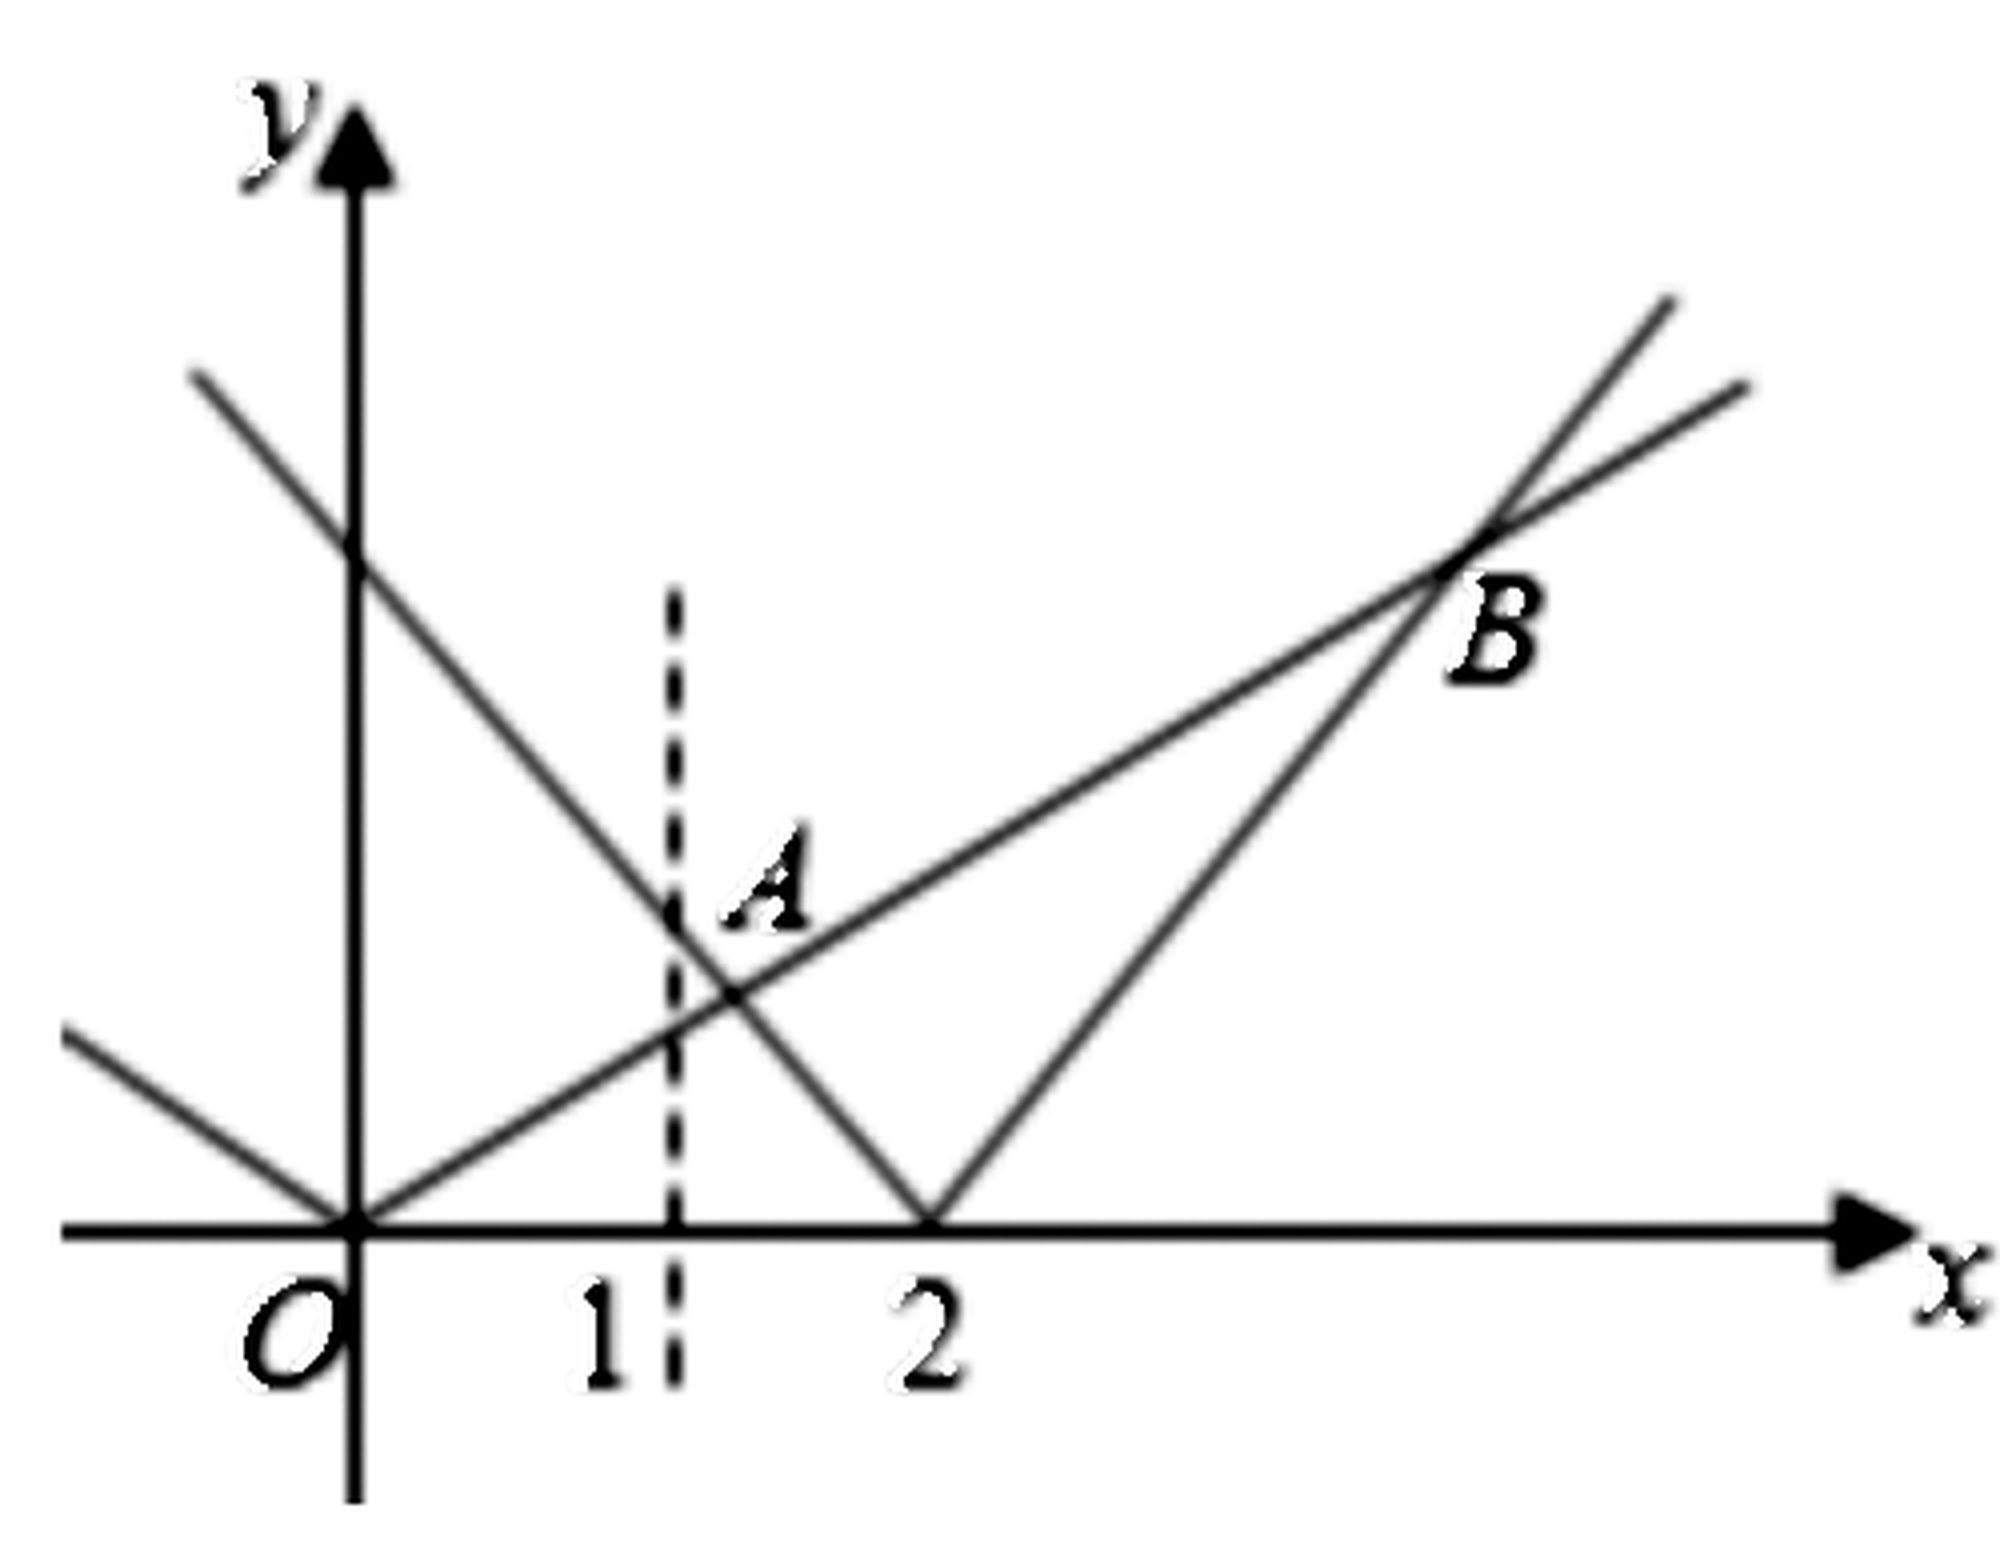
\includegraphics[width=0.40\textwidth]{figures/gao152_q15.png}
\end{center}
\step{由 $0<k<1$，得 $x_A>1$，}
\step{所以关于 $x$ 的不等式 $k\lvert x\rvert-\lvert x-2\rvert>0$ 恰好有 4 个整数解，是 2，3，4，5，}
\step{由 $\begin{cases}y=kx\\y=x-2\end{cases}\Rightarrow x_B=\dfrac2{1-k}\in(5,6]$，故 $\dfrac35<k\leqslant\dfrac23$；故选 $B$.}
\solend
\fi

% === Q16 === 咖啡优惠题；解析 12 行（跨 04 页上下半）；故选 C
\item 上海是全球咖啡店最多的城市. 若某品牌的某种在售咖啡产品价格为 30 元/杯，其原材料成本为 7 元/杯，营销成本为 5 元/杯，且该品牌门店提供如下 4 种优惠方式：(1) 首杯免单，每人限用一次；(2) 3.8 折优惠券，每人限用一次；(3) 买 2 杯送 2 杯，每人限用两次；(4) 买 5 杯送 5 杯，不限使用人数和使用次数. 每位消费者都可以在以上 4 种优惠方式中选择不多于 2 种使用. 现在某个公司有 5 位后勤工作人员去该品牌门店帮每位技术人员购买 1 杯咖啡，购买杯数与技术人员人数须保持一致；请问，这个公司的技术人员不少于\mbox{（\quad）}人时，无论 5 位后勤人员采用什么样的优惠方式购买咖啡，这笔订单该品牌门店都能保证盈利.

\keepwithprev
A. 20\qquad\qquad B. 25\qquad\qquad C. 30\qquad\qquad D. 35

\ifanswer
\solbegin
\step{按各优惠不叠加于同一杯理解，3.8 折券仅用于一杯，}
\step{买赠中的购买杯按原价付款.}
\step{设共购 $n$ 杯，免单、券购、原价购买的杯数分别为 $a,b,c$，其中 $0\leqslant a,b\leqslant5$，}
\step{其余为买赠咖啡，每杯成本为 12 元，}
\step{利润为 $P=15(n-a-b-c)+11.4b+30c-12n=3n-15a-3.6b+15c$，}
\step{若 $a,b$ 不同时为 5，则 $15a+3.6b\leqslant75+14.4=89.4$，}
\step{当 $n\geqslant30$ 时，$P\geqslant90-89.4=0.6>0$.}
\step{若 $a=b=5$，则每人均已使用免单和优惠券两种方式，其余均须原价购买，}
\step{$P=57+30(n-10)-12n=18n-243\geqslant297>0$.}
\step{当 $n=29$ 时，4 人各用方式 (1)(2) 购得 2 杯，}
\step{另 1 人用方式 (1) 及两次方式 (4) 购得 21 杯，}
\step{此时 $P=4\times11.4+2\times150-29\times12=-2.4<0$，因此最小人数为 30，故选 $C$.}% $2\times150$ 为两次方式（4）各买 5 杯的付款，照录（见 ⑤ 3）
\solend
\fi

\end{enumerate}

\bigsec{三、解答题}

\begin{enumerate}
\setcounter{enumi}{16}

% === Q17 === 解集含 \R／\varnothing；解析 4 行
\item 若 $a$、$b\in\R$，求关于 $x$ 的不等式 $ax\geqslant b$ 的解集.

\ifanswer
\solbegin
\step{当 $a>0$ 时，原不等式的解集为 $\left\{x\mid x\geqslant\dfrac ba\right\}$；}
\step{当 $a<0$ 时，原不等式的解集为 $\left\{x\mid x\leqslant\dfrac ba\right\}$；}
\step{当 $a=0$，$b\leqslant0$ 时，原不等式的解集为 $\R$；}
\step{当 $a=0$，$b>0$ 时，原不等式的解集为 $\varnothing$.}
\solend
\fi

% === Q18 === 子集 ⊆ 两处照录；cases 块；解析 9 行（跨 05 页上下半）
\item 已知 $\alpha:x<3m-1$ 或 $x>-m$，$\beta:x<2$ 或 $x\geqslant4$.

(1) 若 $\alpha$ 是 $\beta$ 的充分条件，求实数 $m$ 的取值范围；

(2) 若 $\alpha$ 是 $\beta$ 的必要条件，求实数 $m$ 的取值范围.

\ifanswer
\solbegin
\step{(1) 设 $A=\{x\mid x<3m-1\text{ 或 }x>-m\}$，$B=\{x\mid x<2\text{ 或 }x\geqslant4\}$，}
\step{因为 $\alpha$ 是 $\beta$ 的充分条件，所以 $A\subseteq B$，}
\step{当 $3m-1>-m$ 时，即 $m>\dfrac14$，此时 $A=\R$，不满足题意；}
\step{当 $3m-1\leqslant-m$ 时，即 $m\leqslant\dfrac14$，有 $\begin{cases}3m-1\leqslant2\\-m\geqslant4\end{cases}$，解得 $m\leqslant-4$；}
\step{综上，$m$ 的取值范围为 $(-\infty,-4]$.}
\step{(2) 因为 $\alpha$ 是 $\beta$ 的必要条件，所以 $B\subseteq A$，}
\step{当 $3m-1>-m$ 时，即 $m>\dfrac14$，此时 $A=\R$，$B\subseteq A$ 成立；}
\step{当 $3m-1\leqslant-m$ 时，即 $m\leqslant\dfrac14$，有 $\begin{cases}3m-1\geqslant2\\-m<4\end{cases}$，无解.}
\step{综上，$m$ 的取值范围为 $\left[\dfrac14,+\infty\right)$.}
\solend
\fi

% === Q19 === \varnothing 空集照录；解析 9 行
\item 设关于 $x$ 的不等式 $x^2+4x+k-1\geqslant0$ 的解集为 $A$.

(1) 若 $A=\R$，求实数 $k$ 的取值范围；

(2) 求证：不存在实数 $k$，使得 $A=\varnothing$.

\ifanswer
\solbegin
\step{(1) 配方得 $x^2+4x+k-1=(x+2)^2+k-5$，}
\step{若 $A=\R$，取 $x=-2$，得 $k-5\geqslant0$，即 $k\geqslant5$.}
\step{当 $k\geqslant5$ 时，对任意 $x\in\R$，都有 $(x+2)^2+k-5\geqslant0$，因此 $A=\R$.}
\step{所以 $k$ 的取值范围为 $[5,+\infty)$.}
\step{(2) 当 $k\geqslant5$ 时，由 (1) 得 $A=\R\ne\varnothing$.}
\step{当 $k<5$ 时，取 $x_0=-2+\sqrt{5-k}$，}
\step{则 $x_0^2+4x_0+k-1=(x_0+2)^2+k-5=(5-k)+k-5=0$，}
\step{所以 $x_0\in A$，即 $A\ne\varnothing$.}
\step{因此，不存在实数 $k$，使得 $A=\varnothing$.}
\solend
\fi

% === Q20 === |A\cap B|=1 印等号；等腰偏高粗 \Delta 照录；解析 12 行（跨 06→07 页）
\item 设 $m\in\R$. 集合 $A=\left\{x\mid\dfrac{x^2+x}{x+1}\geqslant\dfrac{2x+m}{x},x\in\R\right\}$，
$B=\left\{x\mid\dfrac{x^2+x}{x+1}\leqslant\dfrac{2x+m}{x},x\in\R\right\}$.

(1) 若 $m=8$，记集合 $M=A\cap(0,+\infty)$，求集合 $M$；

(2) 用 $\lvert T\rvert$ 代表集合 $T$ 的元素个数. 若 $\lvert A\cap B\rvert=1$，记 $m$ 的取值集合为 $C$，试比较 $\lvert C\rvert$ 与 2 的大小，并证明你的结论.

\ifanswer
\solbegin
\step{(1) 当 $m=8$，$x>0$ 时，$\dfrac{x^2+x}{x+1}\geqslant\dfrac{2x+8}{x}\Leftrightarrow x^2-2x-8\geqslant0$}
\step{$\Leftrightarrow(x-4)(x+2)\geqslant0\Leftrightarrow x\geqslant4$，所以 $M=[4,+\infty)$.}
\step{(2) 原分式有意义须 $x\ne-1,0$，因此 $x\in A\cap B\Leftrightarrow\begin{cases}x^2-2x-m=0\\x\ne-1,0\end{cases}$，}
\step{方程的判别式为 $\Delta=4(1+m)$.}
\step{当 $m<-1$ 时，方程无实根，$\lvert A\cap B\rvert=0$；}
\step{当 $m=-1$ 时，方程只有一个实根 1，$A\cap B=\{1\}$.}
\step{当 $m>-1$ 时，方程有两个不同实根.}
\step{其中，0 为根当且仅当 $m=0$，$-1$ 为根当且仅当 $m=3$.}
\step{$m=0$ 时，方程的根为 $0,2$，$A\cap B=\{2\}$；}
\step{$m=3$ 时，方程的根为 $-1,3$，$A\cap B=\{3\}$.}
\step{$m>-1$ 且 $m\ne0,3$ 时，两个实根均满足原分式的定义条件，$\lvert A\cap B\rvert=2$.}
\step{因此 $C=\{-1,0,3\}$，$\lvert C\rvert=3>2$.}
\solend
\fi

% === Q21 === "性质 p"新定义、\Q 归一、M\subseteq\R 照录；解析 19 行（跨 07→08 页）
\item 设集合 $M\subseteq\R$. 若 $M$ 中元素个数大于等于 2，且 $M$ 的任意不同元素 $a$、$b$ 均满足 $a^3-\dfrac14b\in M$，则称集合 $M$ 具有“性质 $p$”.

(1) 试判断集合 $\Q$、集合 $\left\{-\dfrac{\sqrt3}{2},0,\dfrac{\sqrt3}{2}\right\}$ 是否具有“性质 $p$”，并说明理由；

(2) 设 $m$ 为大于等于 2 的正整数. 若集合 $A=\{x_1,x_2,\cdots,x_m\}$，且具有“性质 $p$”，求证：$m=2$，并求集合 $A$ 中所有元素的乘积.

\ifanswer
\solbegin
\step{(1) $\Q$ 中至少有两个元素，且任意不同的 $a,b\in\Q$ 均满足 $a^3-\dfrac14b\in\Q$，}
\step{故 $\Q$ 具有“性质 $p$”.}
\step{对于另一集合，取 $a=0$，$b=\dfrac{\sqrt3}{2}$，则 $a^3-\dfrac14b=-\dfrac{\sqrt3}{8}$ 不属于该集合，}
\step{故其不具有“性质 $p$”.}
\step{(2) 将 $A$ 中元素按 $x_1<x_2<\cdots<x_m$ 排列.}
\step{若 $m\geqslant3$，由性质 $p$ 及幂函数 $y=x^3$ 的单调性，}
\step{有 $x_1^3-\dfrac14x_m<\cdots<x_1^3-\dfrac14x_2<x_m^3-\dfrac14x_2<x_m^3-\dfrac14x_1$，}
\step{上述 $m+1$ 个互不相同的数均属于 $A$，与 $A$ 只有 $m$ 个元素矛盾，}
\step{因此 $m=2$.}
\step{设 $A=\{a,b\}$，$a<b$.}
\step{因为 $a^3-\dfrac14b<b^3-\dfrac14a$，且两者均属于 $A$，}
\step{所以 $a^3-\dfrac14b=a$，$b^3-\dfrac14a=b$，}
\step{两式相减并除以 $a-b\ne0$，}
\step{以及两式相加，分别得 $a^2+ab+b^2=\dfrac34$，$(a+b)(a^2-ab+b^2)=\dfrac54(a+b)$，}
\step{代入 $a^2-ab+b^2=\dfrac34-2ab$，得 $(a+b)(4ab+1)=0$，}
\step{若 $a+b=0$，则 $-ab=a^2+ab+b^2=\dfrac34$，即 $ab=-\dfrac34$；}
\step{若 $a+b\ne0$，则 $ab=-\dfrac14$.}
\step{分别取 $A=\left\{-\dfrac{\sqrt3}{2},\dfrac{\sqrt3}{2}\right\}$，$A=\left\{\dfrac{1-\sqrt3}{2\sqrt2},\dfrac{1+\sqrt3}{2\sqrt2}\right\}$，}
\step{代入均有 $a^3-\dfrac14b=a$、$b^3-\dfrac14a=b$，故两种乘积均可取得.}
\solend
\fi

\end{enumerate}

\end{document}
